%Plantilla basada en "Template for Masters / Doctoral Thesis" (plantilla disponible en writeLaTex) que subió LaTeXTemplates.com

\documentclass[a4paper]{book}
\usepackage[paperwidth=17cm, paperheight=22.5cm, bottom=2.5cm, right=2.5cm]{geometry}
\usepackage{amssymb,amsmath,amsthm} %paquete para símbolo matemáticos
\usepackage[spanish]{babel}
\usepackage[utf8]{inputenc} %Paquete para escribir acentos y otros símbolos directamente
\usepackage{enumerate}
\usepackage{graphicx}
%\usepackage{subfig} %para poner subfiguras
\graphicspath{{Img/}} %En qué carpeta están las imágenes
\usepackage[nottoc]{tocbibind}
\usepackage[pdftex,
            pdfauthor={NOMBRE DEL AUTOR},
            pdftitle={TÍTULO DE LA TESIS},
            pdfsubject={ÁREA DE LA TESIS},
            pdfkeywords={PALABRAS CLAVE},
            pdfproducer={Latex con hyperref},
            pdfcreator={pdflatex}]{hyperref}



\begin{document}

%----------------------------------------------------------------------------------------
%	COMANDOS PERSONALIZADOS
%----------------------------------------------------------------------------------------

%SI TU TESIS TIENE TEOREMAS Y DEMOSTRACIONES, PUEDES DESCOMENTAR Y USAR LOS SIGUIENTES COMANDOS

%\renewcommand{\proofname}{Demostración}
%\providecommand{\norm}[1]{\lVert#1\rVert} %Provee el comando para producir una norma.
%\providecommand{\innp}[1]{\langle#1\rangle} 
%\newcommand{\seno}{\mathrm{sen}}
%\newcommand{\diff}{\mathrm{d}}

%\newtheorem{teo}{Teorema}[section] 
%\newtheorem{cor}[teo]{Corolario}
%\newtheorem{lem}[teo]{Lema}

%\theoremstyle{definition}
%\newtheorem{dfn}[teo]{Definición}

%\theoremstyle{remark}
%\newtheorem{obs}[teo]{Observación}

%\allowdisplaybreaks



%----------------------------------------------------------------------------------------
%	PORTADA
%----------------------------------------------------------------------------------------

\title{TesisMaxi} %Con este nombre se guardará el proyecto en writeLaTex

\begin{titlepage}
\begin{center}

\textsc{\Large Facultad de Inveniería \- Universidad Nacional de Mar del Plata}\\[4em]

\vspace{4em}

\textsc{\huge \textbf{Sistemas Complejos, Ruidos Discretos y su implementación en FPGA}}\\[4em]

\textsc{\large Tesis}\\[1em]

\textsc{para obtener el título de}\\[1em]

\textsc{Doctor en Ingeniería con Orientación en Electrónica}\\[1em]

%\textsc{presenta}\\[1em]

\textsc{\Large Maximiliano Antonelli}\\[1em]

%\textsc{\large Asesor: NOMBRE}

\end{center}

\vspace*{\fill}
\textsc{Mar del Plata, Argentina \hspace*{\fill} 2016}

\end{titlepage}

%----------------------------------------------------------------------------------------
%	DEDICATORIA
%----------------------------------------------------------------------------------------

\pagestyle{empty}
\frontmatter

\chapter*{}
\begin{flushright}
\textit{A Sonia y Eduardo, que hicieron la mejor versión de mí que pudieron.\\
A Lorena, que sigue intentándolo.\\
A Giuliana y Luca, que les sale sin querer.}
\end{flushright}

%----------------------------------------------------------------------------------------
%	AGRADECIMIENTOS
%----------------------------------------------------------------------------------------

\chapter*{Agradecimientos}
%\markboth{AGRADECIMIENTOS23}{AGRADECIMIENTOS} % encabezado 

¡Muchas gracias a todos!

\tableofcontents


%----------------------------------------------------------------------------------------
%	TESIS
%----------------------------------------------------------------------------------------
\mainmatter %empieza la numeración de las páginas
\pagestyle{headings}

%  Incluye los capítulos en el folder de capítulos

\chapter{Introducción}

Los números aleatorios constituyen una de las bases del desarrollo tecnológico, han sido utilizados exitosamente en una gran variedad de aplicaciones como juegos, criptografía, modelado de sistemas físicos, sistemas biológicos, etc.
Éstos pueden ser generados a partir de fuentes de aleatoriedad de naturaleza física (TRNG) o a partir de generadores algorítmicos (PRNG).
En esta tesis se propone reemplazar los generadores algorítmicos por sistemas caóticos, aunque las secuencias generadas por estos últimos requieren un postprocesamiento para mejorar sus propiedades aleatorias.

Esta tesis se centra en la implementación en hardware electrónico de RNGs, particularmente se trata de responder dos preguntas principales: ¿Cómo varían las propiedades estadísticas de los sistemas caóticos cuando son implementados en hardware digital? y, ¿Es posible implementar un generador físico de ruido en hardware?
La primer pregunta está directamente relacionada con generadores PRNG, la segunda apunta a la posibilidad de implementar un TRNG (analógico) en hardware digital.

Para estudiar los RNGs, se utilizaron cuantificadores de la teoría de la información, por un lado basados en entropías de valores y por otro en entropías de patrones de orden.
Estas dos entropías son complementarias y cubren los dos principales aspectos a considerar: estocasticidad de los valores generados e  independencia esadística de valores consecutivos.
Además se utilizan exponentes de Lyapunov para evaluar la caoticidad de los sistemas implementados en hardware.

Cuando un sistema es calculado en aritmética discreta, el resultado de cada iteración se sustituye por el valor representable más cercano, lo que desvía su trayectoria de la que tendría utilizando números reales.
La inherente sensibilidad a las condiciones iniciales que presentan los sistemas caóticos hace que estas perturbaciones se vean amplificadas con cada iteración (vía el máximo exponente de Lyapunov) y el sistema resultante pueda tener poco que ver con el original.
En el mejor de los casos el sistema pasa a ser pseudocaótico y sus propiedades como estocasticidad, mezcla, período y caoticidad se ven degradadas.
Uno de los aportes de la tesis es el estudio de esta degradación en función de la granularidad de la aritmética representada en un sistema electrónico digital.

Por el lado de los TRNG, está bien establecido que un oscilador en anillo (RO) presenta fluctuaciones de fase (jitter) que dependen de procesos puramente físicos como gradientes durante el proceso de difusión en la fabricación del circuito integrado, gradientes en la temperatura de trabajo, ruido térmico en las junturas semiconductoras, etc.
Como los ROs son comúnmente utilizados como generadores de señales de reloj para sincronizar sistemas, el jitter suele ser un problema.
Sin embargo en esta tesis son la fuente de aleatoriedad física que utilizamos para generar señales estocásticas.
Se propuso un método basado en entropías diferenciales que permite extraer un valor que indica la aleatoriedad de una serie binaria y, por lo tanto, puede indicar el nivel de jitter que contiene.
Este método es útil para catalogar un dado RO como bueno para generar ruido o como señal de reloj.
Además, se implementó un TRNG basado en ROs mediante la mezcla de varios osciladores.

El primer capítulo (cap. \ref{capSist}) es una introducción a los sistemas dinámicos caóticos utilizados a lo largo de la tesis.
El segundo capítulo (cap. \ref{capCuanti}) contiene, por un lado una introducción a los cuantificadores de aleatoriedad que se utilizan para medir los generadores de números, y por otro, algunos avances en la implementación de estos cuantificadores en hardware electrónico (FPGA).
El capítulo \ref{capGen} presenta algunos avances en generadores de números aleatorios utilizando sistemas caóticos y sus aplicaciones.
En el capítulo \ref{capSwitch} se estudia la degradación estadística de los mapas caóticos cuando son implementados en aritmética discreta.
Y por último en el capítulo \ref{capRings}, primero se propone la utilización de cauntificadores de la teoría de la información para medir la mezcla y estocasticidad de la fuente de incertezas en RO's, luego se muestran los resultados de la implementación en FPGA de un TRNG utilizando RO's.
\thispagestyle{empty}

\chapter{Generadores de Números Aleatorios}

%%%%%%%%%%%%%%%%%%%%%%%%%%%%%%%%%%%%%%%%%%%%%%%%%%%%%%%%%%%%%%%%%%%%%%%%%%%%%
\section{Cripto-Codificación caótica Variante en el tiempo}

\subsection{Introdución}

En los sistemas de comunicaciones y particularmente en los
dedicados a la codificación para el control de error y
encriptamiento de datos se usan técnicas derivadas de la teoría de
señales. Estas técnicas se aplican típicamente en la forma lineal
debido a la simplicidad que ésto trae aparejado. Además cada una se
implementa algorítmicamente o físicamente como una entidad
independiente. Para cada sistema en particular se las elige
con criterios de conveniencia práctica, y se las aplica en forma
consecutiva o encadenada. La teoría de los sistemas no lineales
\cite{Strogatz1994,Lasota1994} aparece como un marco de trabajo
ideal para ser utilizado en el contexto anteriormente mencionado.
La existencia de los sistemas caóticos, y la relación de estos con
la aleatoriedad, o pseudo aleatoriedad, otorga una plataforma de
diseño que hasta hoy se encuentra poco explotada.

En los últimos veinte años se han presentado diversos trabajos que
emplean caos en los sistemas de comunicaciones, como por ejemplo
el empleo de portadoras caóticas sincronizadas en las
transmisiones analógicas \cite{Kocarev1995,Hidalgo2001}. Si nos
centramos en la representación discreta un referente muy
importante es el excelente trabajo de Kozic et. als.
\cite{Kozic2006A,Kozic2006B} en el que se presenta una técnica de
modulación empleando mapas caóticos unidimensionales lineales por
tramos, la técnica consiste en la introduccíón del mensaje a
codificar en el bit menos significativo de la secuencia generada.
Obteniéndose una secuencia levemente alterada lo que impide que el
sistema entre en ciclos periódicos.

En este trabajo se propone un grupo de atractores como generadores de señales
pseudoaleatorias para realizar el proceso de codificación y
encriptamiento. El esquema de codificación se basa
en una familia de mapas cuadráticos bidimensionales, cuyas salidas
presentan comportamiento caótico, con distintos atractores
conforme a los coeficientes que se empleen. La idea es que cada
palabra a codificar sea unívoca con un juego de coeficientes que
serán parámetros de un mapa cuadrático bidimensional. Como
resultado de este procedimiento, la señal de salida son puntos
pertenecientes a distintos atractores elegidos por la información
a transmitir.

La ventaja de este método reside en que la
estructura de toda la familia de mapas es única y común, modificándose
solamente los coeficientes se consiguen atractores distintos. Esta
priopiedad reduce y facilita la implementación en hardware.
Resultados preliminares obtenidos mediante simulaciones muestran
que el sistema presenta una performance comparable a la
obtenida en sistemas clásicos de encriptamiento, en cuanto a
probabilidad de error y a distancia mínima.


\subsection{Mapas cuadráticos bidimensionales}


En este trabajo se emplea una familia de mapas cuadráticos
bidimensionales cuya estructura consta de dos ecuaciones
cuadráticas en diferencias acopladas (Ec.\ref{eq:Qmap}). La
característica principal de este mapa es que los parámetros, $a_i$
y $b_i$, son coeficientes reales y para ciertos valores de estos
coeficientes la salida del sistema presentará comportamiento
caótico.

Se obtiene así un subgrupo de mapas distintos con comportamiento
caótico según la elección de estos coeficientes, en la Fig.
\ref{fig:atractores} puede verse tres atractores para tres juegos
distintos de valores de los coeficientes.

Estos mapas han sido ampliamente estudiados, por lo que la
estabilidad, la sensibilidad a las condiciones iniciales y su
dimensión fractal son parámetros ya conocidos
\cite{Sprott2003,Sprott2000}.

\begin{eqnarray}\label{eq:Qmap}
    x_{n+1}&=& a_0 + a_1 x_n + a_2 x_n^2 + a_3 x_n y_n + a_4 y_n^2 + a_5 y_n \nonumber\\
    y_{n+1}&=& b_0 + b_1 x_n + b_2 x_n^2 + b_3 x_n y_n + b_4 y_n^2 + b_5 y_n
\end{eqnarray}

%hablar sobre mapas perturbados por la información
\begin{figure}
    \centering
    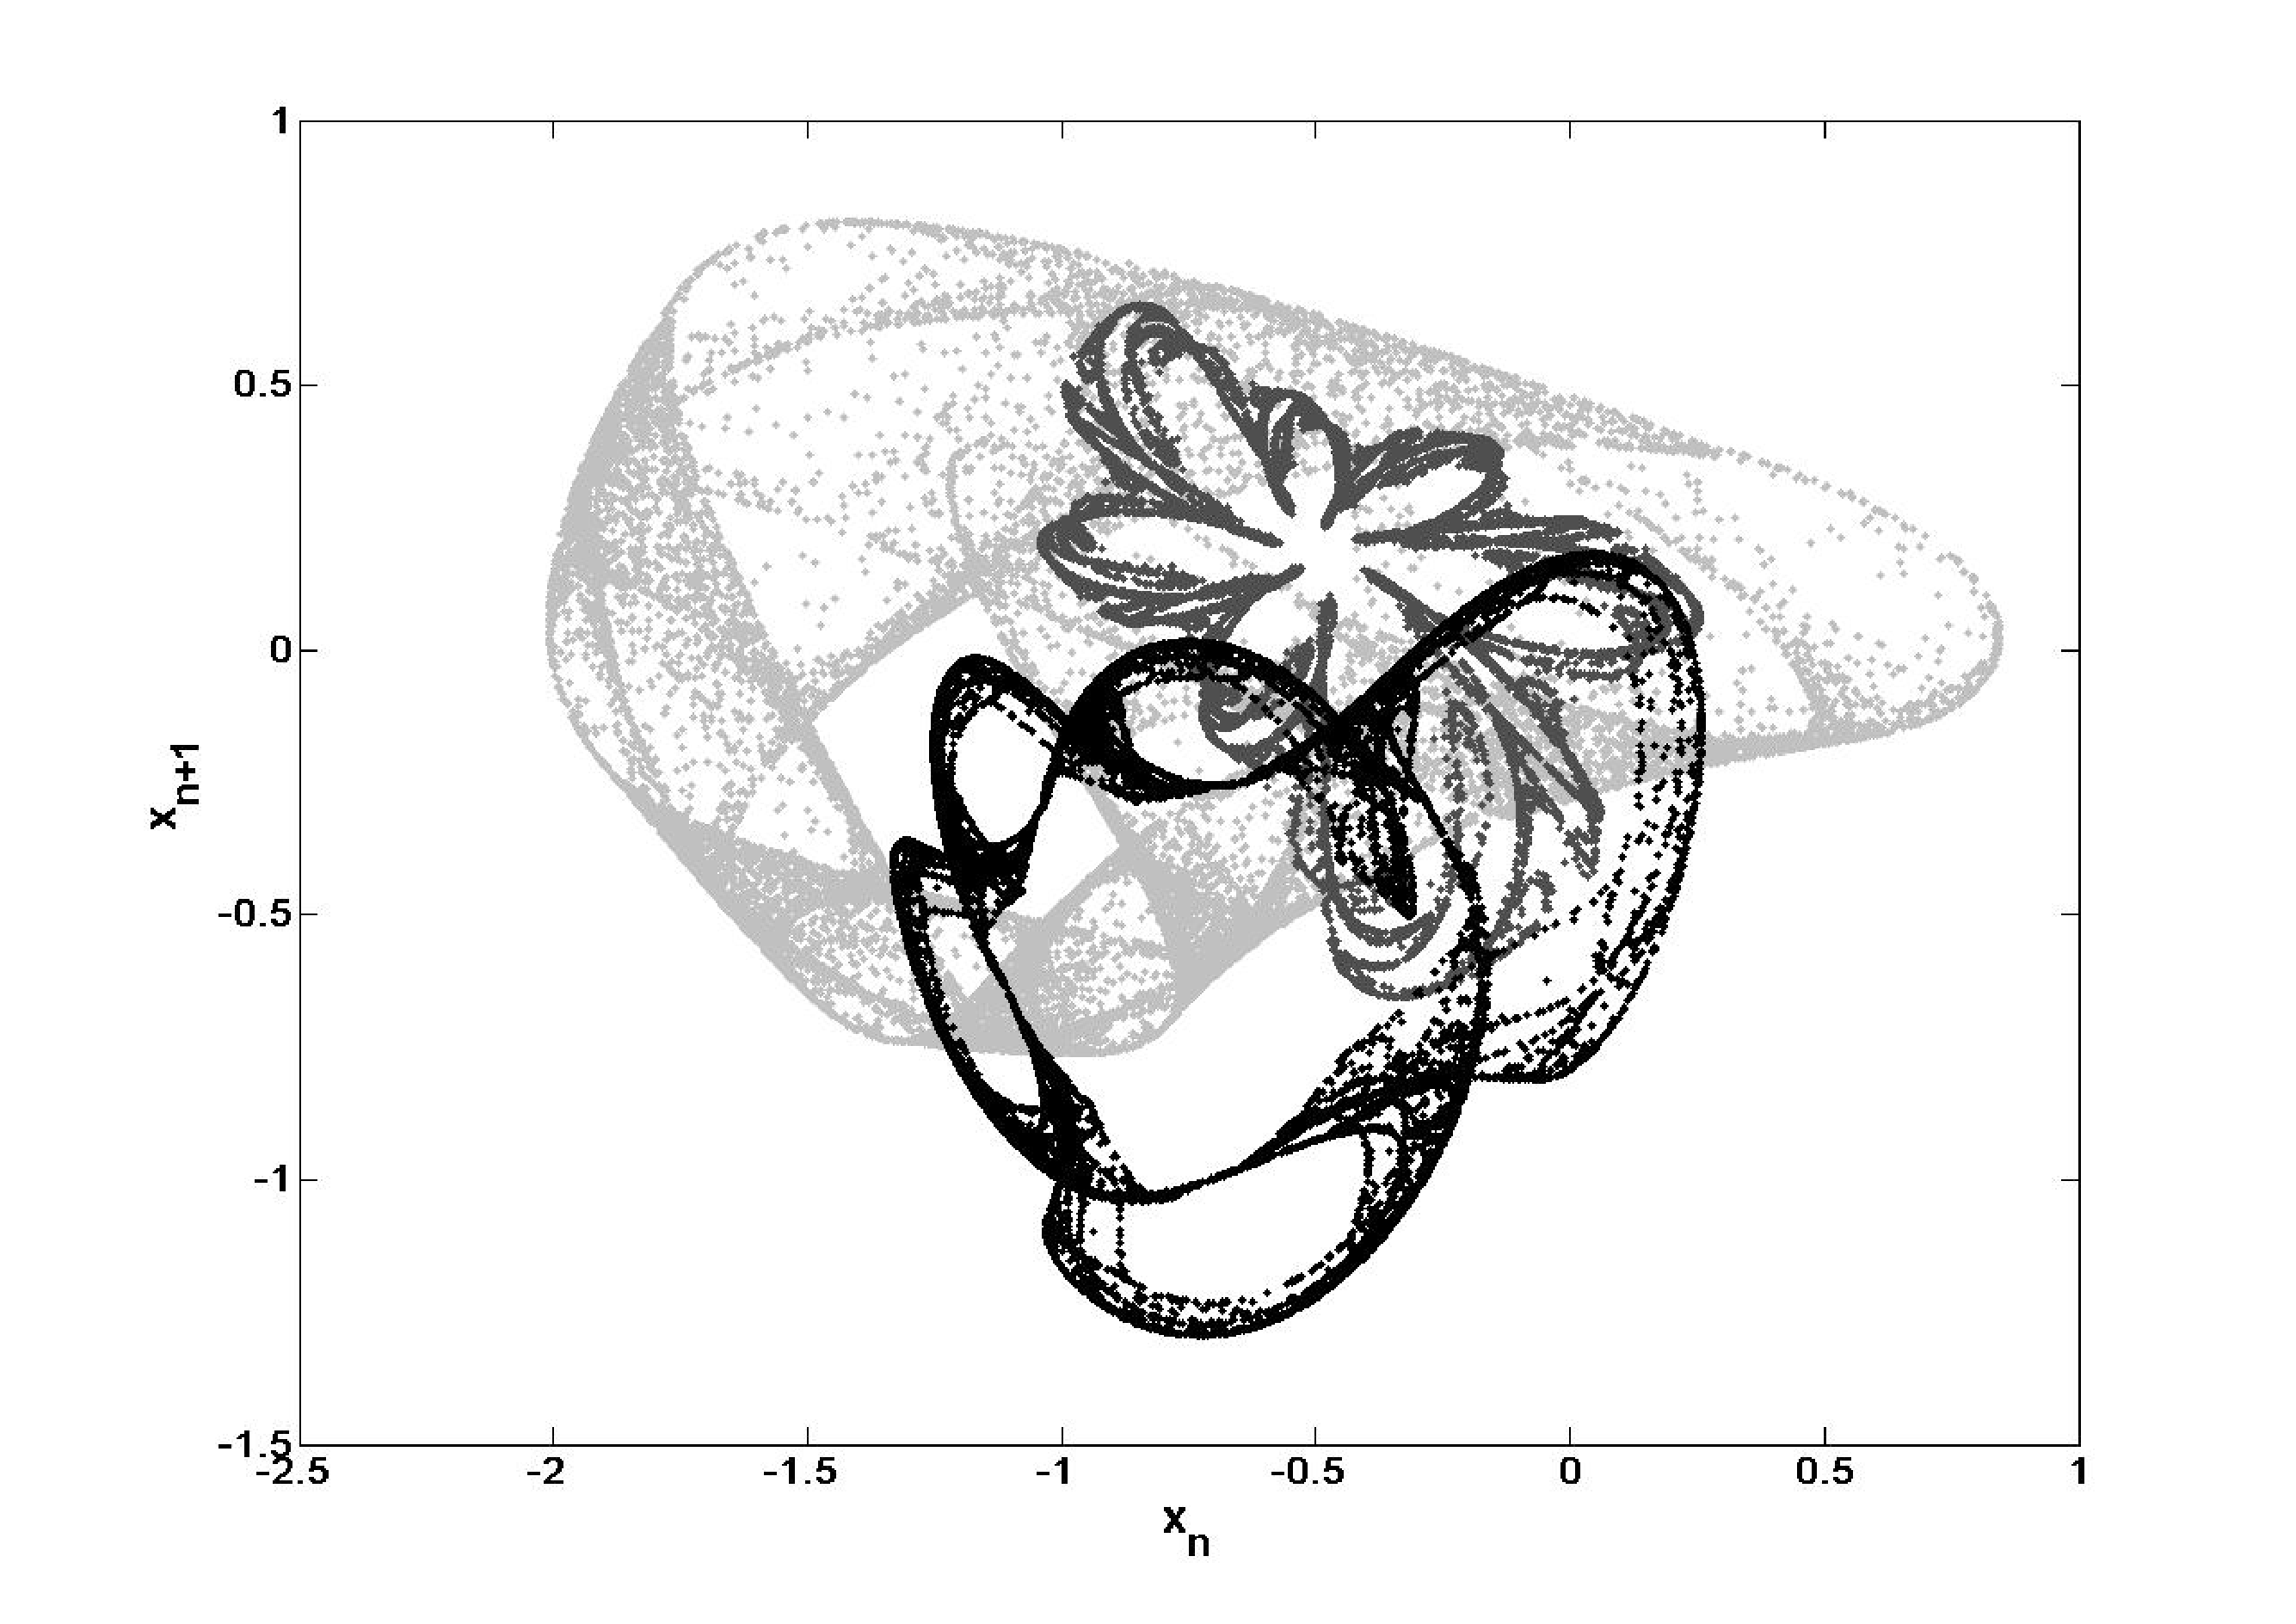
\includegraphics[width=1\columnwidth]{atractores.pdf}\\
    \caption{Atractores del sistema para tres juegos de coeficientes.}\label{fig:atractores}
\end{figure}

\subsection{Implementación}

Desde el punto de vista del esquema de codificación propuesto,
estos mapas son muy atractivos por el hecho de contar con $12$
coeficientes para generar cada atractor. Por lo tanto, las
combinaciones posibles serán $N^{12}$, en donde $N$ es la cantidad
de símblos posibles según la aritmética utilizada. En nuestro caso
empleamos una aritmética de $19$ bits expresados en complemento a
$2$ con aritmética de punto fijo, con $1$ bit de signo, $3$ bits
de parte entera y $15$ bits de parte decimal. Esta aritmética
limita y discretiza el plano $xy$ que queda delimitado por $\Delta
x=4$, $-\Delta x=-4$, $\Delta y=4$,$-\Delta y=-4$, como puede
verse en la figura \ref{fig:atractores}. Estas limitaciones al
plano de atracción tienen como consecuencia dos cuestiones a tener
en cuenta:
\begin{itemize}
    \item
        Debido a que los coeficientes se generan con la misma aritmética que las variables, nos
        encontramos con $N=2^{19}$ valores posibles para cada coeficiente,
        lo que arroja $\left(2^{19}\right)^{12}\cong4,3^{68}$ combinaciones posibles de coeficientes para generar distintos atractores.
    \item
        En cuanto a las trayectorias de los atractores sobre el plano discretizado,
        éstas se tornan periódicas debido a la discretización.
\end{itemize}


No todos los juegos de coeficientes generan atractores caóticos contenidos en el plano dado por la aritmética utilizada. Aunque esto no sería problema para la codificación/decodificación, se eligieron los coeficientes de modo que se generen atractores contenidos en el plano a modo de validación visual.

Dada la naturaleza de los mapas caóticos, un punto muy lejano a la zona de atracción puede hacer que el punto calculado para la próxima iteración diverja, por lo tanto las condiciones iniciales deben ser normalizadas antes de cambiar al mapa siguiente. Para solucionar este problema se utiliza la siguiente estrategia:
 Primero se define el plano mínimo que contiene al atractor. Para
        identificarlo se simularon los mapas mediante Quartus
        generando secuencias de salida lo suficientemente largas como para
        verificar la periodicidad. Luego se analizó este vector de datos
        con Matlab buscando los valores extremos en cada una de las
        variables: $X1_{max}$, $X1_{min}$, $Y1_{max}$, $Y1_{min}$. Estos límites delimitan al plano mínimo que contiene al atractor. La normalización dada por la ecuación \ref{eq:norm_salida} se aplica a la salida $\left(x,y\right)$ para mapear este plano minimo a todo el plano delimitado por la aritmética utilizada de dimensiones $\Delta x$, $-\Delta x$, $\Delta y$, $-\Delta y$.
Segundo, se halla el plano máximo que contiene las condiciones
iniciales que hacen que no diverja la solución sinó que genere el
atractor. Para esto se realizó un programa en Matlab que genera
los atractores desde todas las condiciones iniciales del plano
delimitado y discretizado por la aritmética utilizada, a
continuación se marcan todos los puntos que generan trayectorias
divergantes o bien convergentes a un punto fijo. Este proceso
genera la zona de condiciones iniciales factible para generar
atractores, nuevamente se identificaron los valores máximos y
mínimos del área rectangular máxima que contenga todos sus puntos
como condiciones iniciales factibles $X2_{max}$, $X2_{min}$,
$Y2_{max}$, $Y2_{min}$. La normalización dada por la ecuación
\ref{eq:norm_entrada} se aplica a la entrada de condiciones
iniciales $\left(x_{n-1},y_{n-1}\right)$ para mapear todo el plano
de dimensiones $\Delta x$, $-\Delta x$, $\Delta y$ y $-\Delta y$
al de condiciones iniciales factibles.


El problema de la existencia de puntos fijos para cierto conjunto de
coeficientes y condiciones iniciales queda salvado al perturbar
continuamente al atractor actual con valores afectados por la
información.

Se generó un circuito en VHDL con un total de $16$ juegos de
parámetros seleccionables con la palabra de entrada de $4$ bits
que se desea encriptar. Esta palabra multiplexa estos coeficientes
y alimenta un oscilador que calcula la próxima iteración de datos,
además, este circuito almacena la salida del oscilador y la
realimenta como ``condición inicial" para calcular la iteración
siguiente (Fig. \ref{fig:generador}). Como resultado de este
proceso, la salida encriptada resulta ser el oscilador actual
seleccionado por la palabra de entrada perturbado por la historia
de los mapas seleccionados por las entradas anteriores. Este
circuito de dos bloques se encarga de generar los atractores, por
lo que se lo llama ``generador de atractores".


Para la primer iteración, las condiciones iniciales son $(x;y)=(0.1;0.1)$ para cualquiera de los atractores.



\begin{figure}
    \centering
    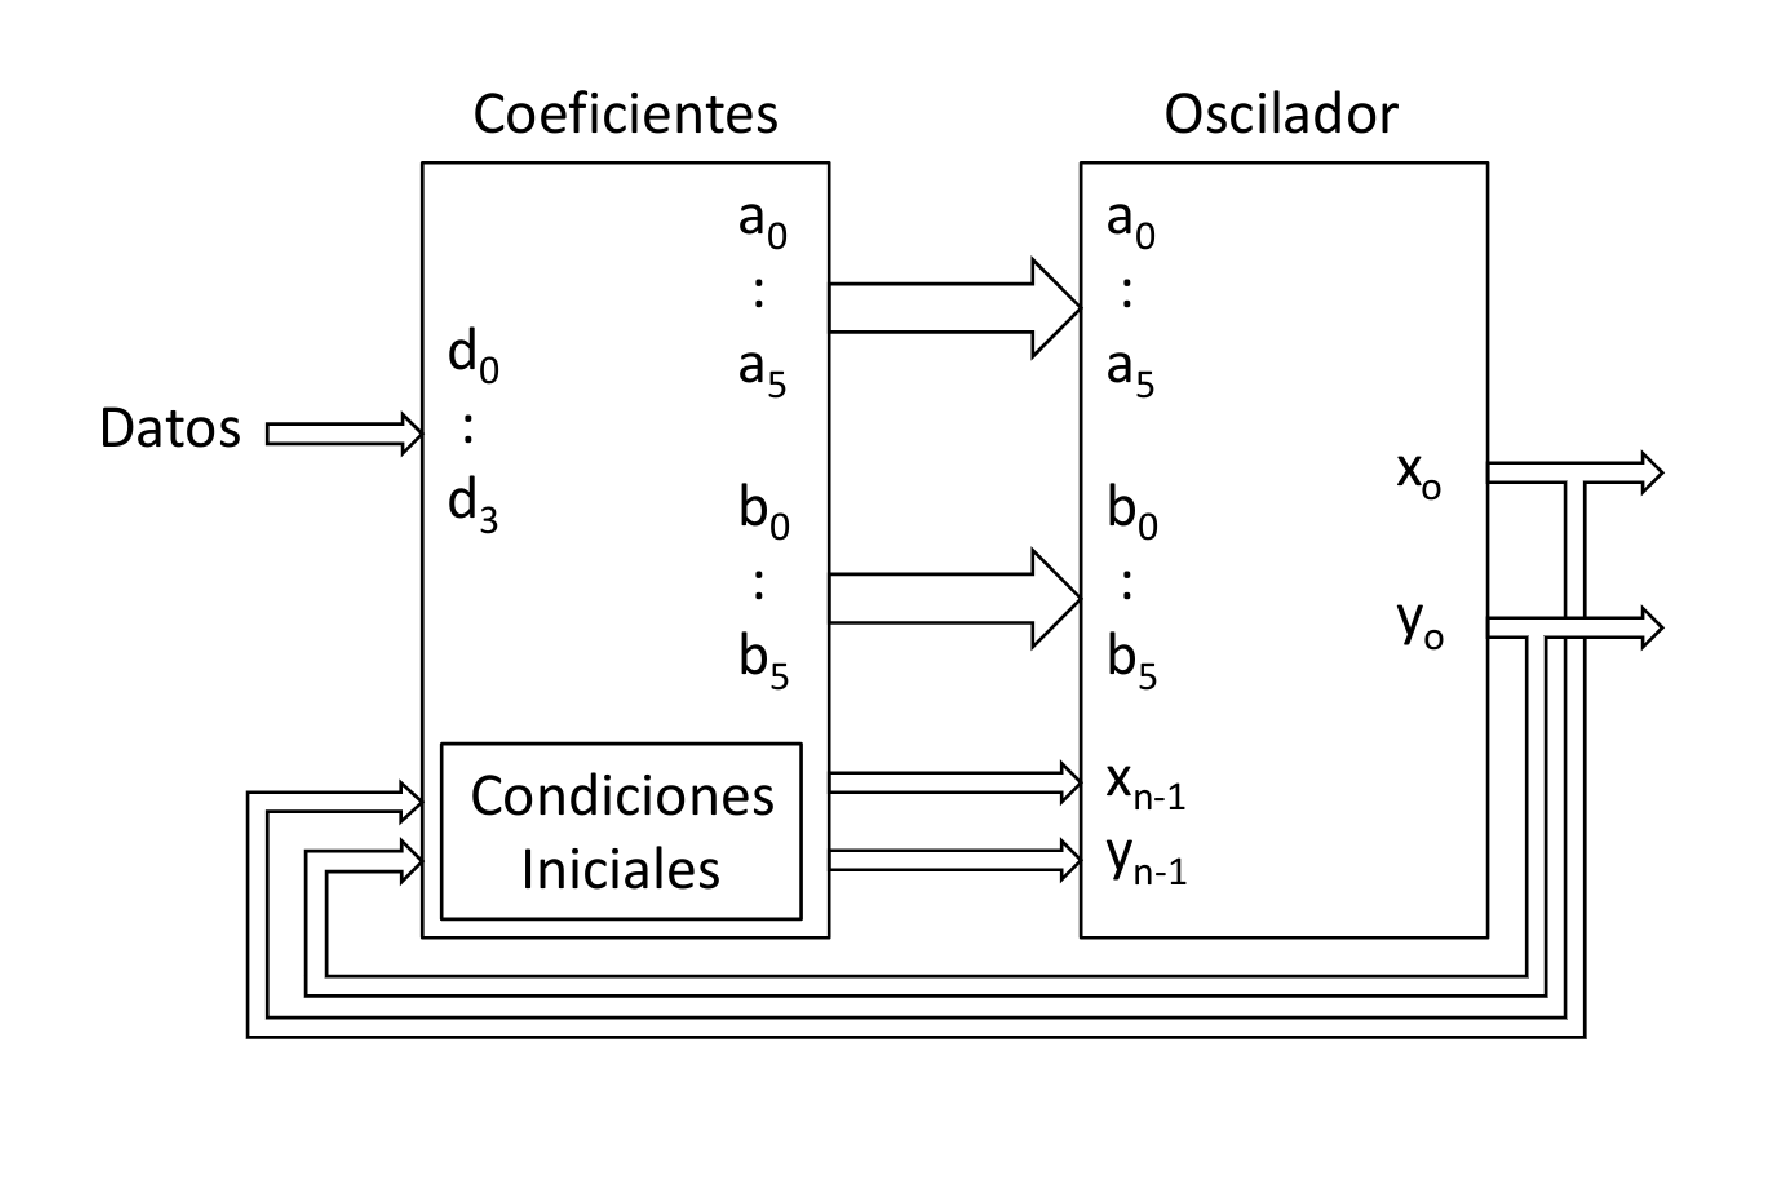
\includegraphics[width=0.7\columnwidth]{Fig1.pdf}\\
    \caption{Generador de atractores.}\label{fig:generador}
\end{figure}
{\small
\begin{eqnarray}\label{eq:norm_salida}
    x_{1norm}&=& a_{1x} x+b_{1x} \nonumber\\
    y_{1norm}&=& a_{1y} y+b_{1x} \nonumber\\
    a_{1x}&=& \frac{2\Delta x}{x1_{max}-x1_{min}} \nonumber\\
    a_{1y}&=& \frac{2\Delta y}{y1_{max}-y1_{min}} \nonumber\\
    b_{1x}&=& -\frac{x1_{max}-x1_{min}}{2} \nonumber\\
    b_{1x}&=& -\frac{y1_{max}-y1_{min}}{2}
\end{eqnarray}}
{\small
\begin{eqnarray}\label{eq:norm_entrada}
    x_{1norm}&=& a_{2x} x+b_{2x} \nonumber\\
    y_{1norm}&=& a_{2y} y+b_{2x} \nonumber\\
    a_{2x}&=& \frac{x2_{max}-x2_{min}}{2\Delta x} \nonumber\\
    a_{2y}&=& \frac{y2_{max}-y2_{min}}{2\Delta y} \nonumber\\
    b_{2x}&=& \frac{x2_{max}-x2_{min}}{2} \nonumber\\
    b_{2x}&=& \frac{y2_{max}-y2_{min}}{2}
\end{eqnarray}}

\subsubsection{Codificador}
El bloque del Codificador consiste en circuito generador y
acondicionamiento de la salida. Para codificar una palabra de
cuatro bits de entrada se generan los valores de $x$ e $y$ con el
circuito generador correspondiente a esta palabra y se los concatena en un circito posterior
formando un vector $[x:y]$ (Fig. \ref{fig:codificador}). De esta forma cada palabra de información a ser enviada será representada por la salida $xy$  del oscilador del atractor correspondiente, por lo tanto una palabra a codificar no se corresponderá con una palabra codificada, dos palabras iguales generarán dos salidas distintas.


\begin{figure}
    \centering
    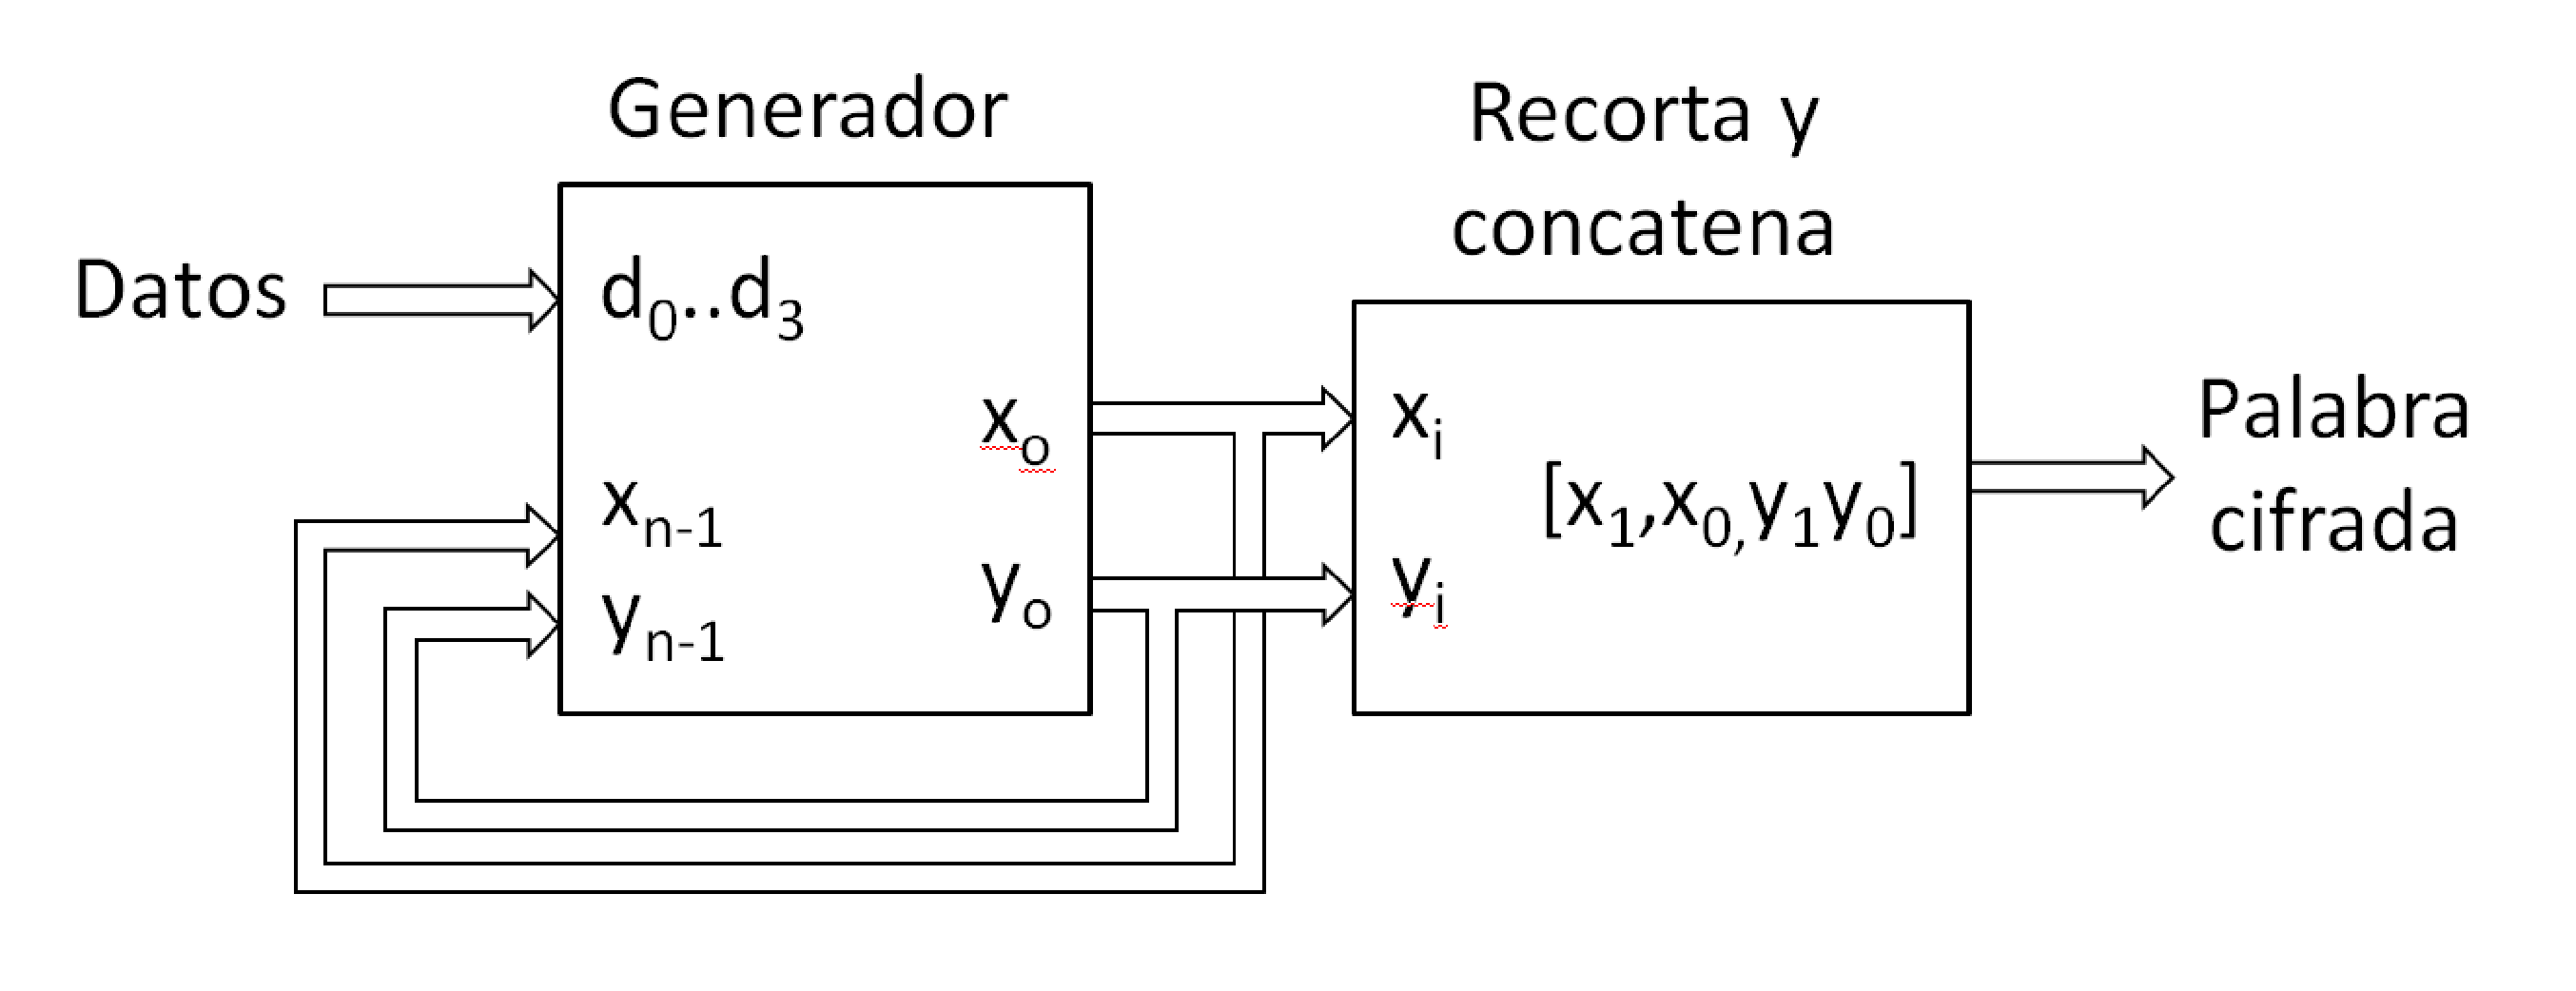
\includegraphics[width=0.8\columnwidth]{Fig2.pdf}\\
    \caption{Codificador.}\label{fig:codificador}
\end{figure}

\subsubsection{Decodificador}


Un segundo circuito generador de atractores funciona en el decodificador generando las $16$ palabras posibles para la próxima iteración. Luego, se ingresan todas estas posibles palabras
cifradas junto con la que se desea decodificar a un comparador que aplica una XOR a la palabra ingresada contra todas las palabras posibles generadas localmente para decodificarla. La
salida de este circuito es la palabra decodificada (Fig. \ref{fig:decodificador}).

\begin{figure}\
    \centering
    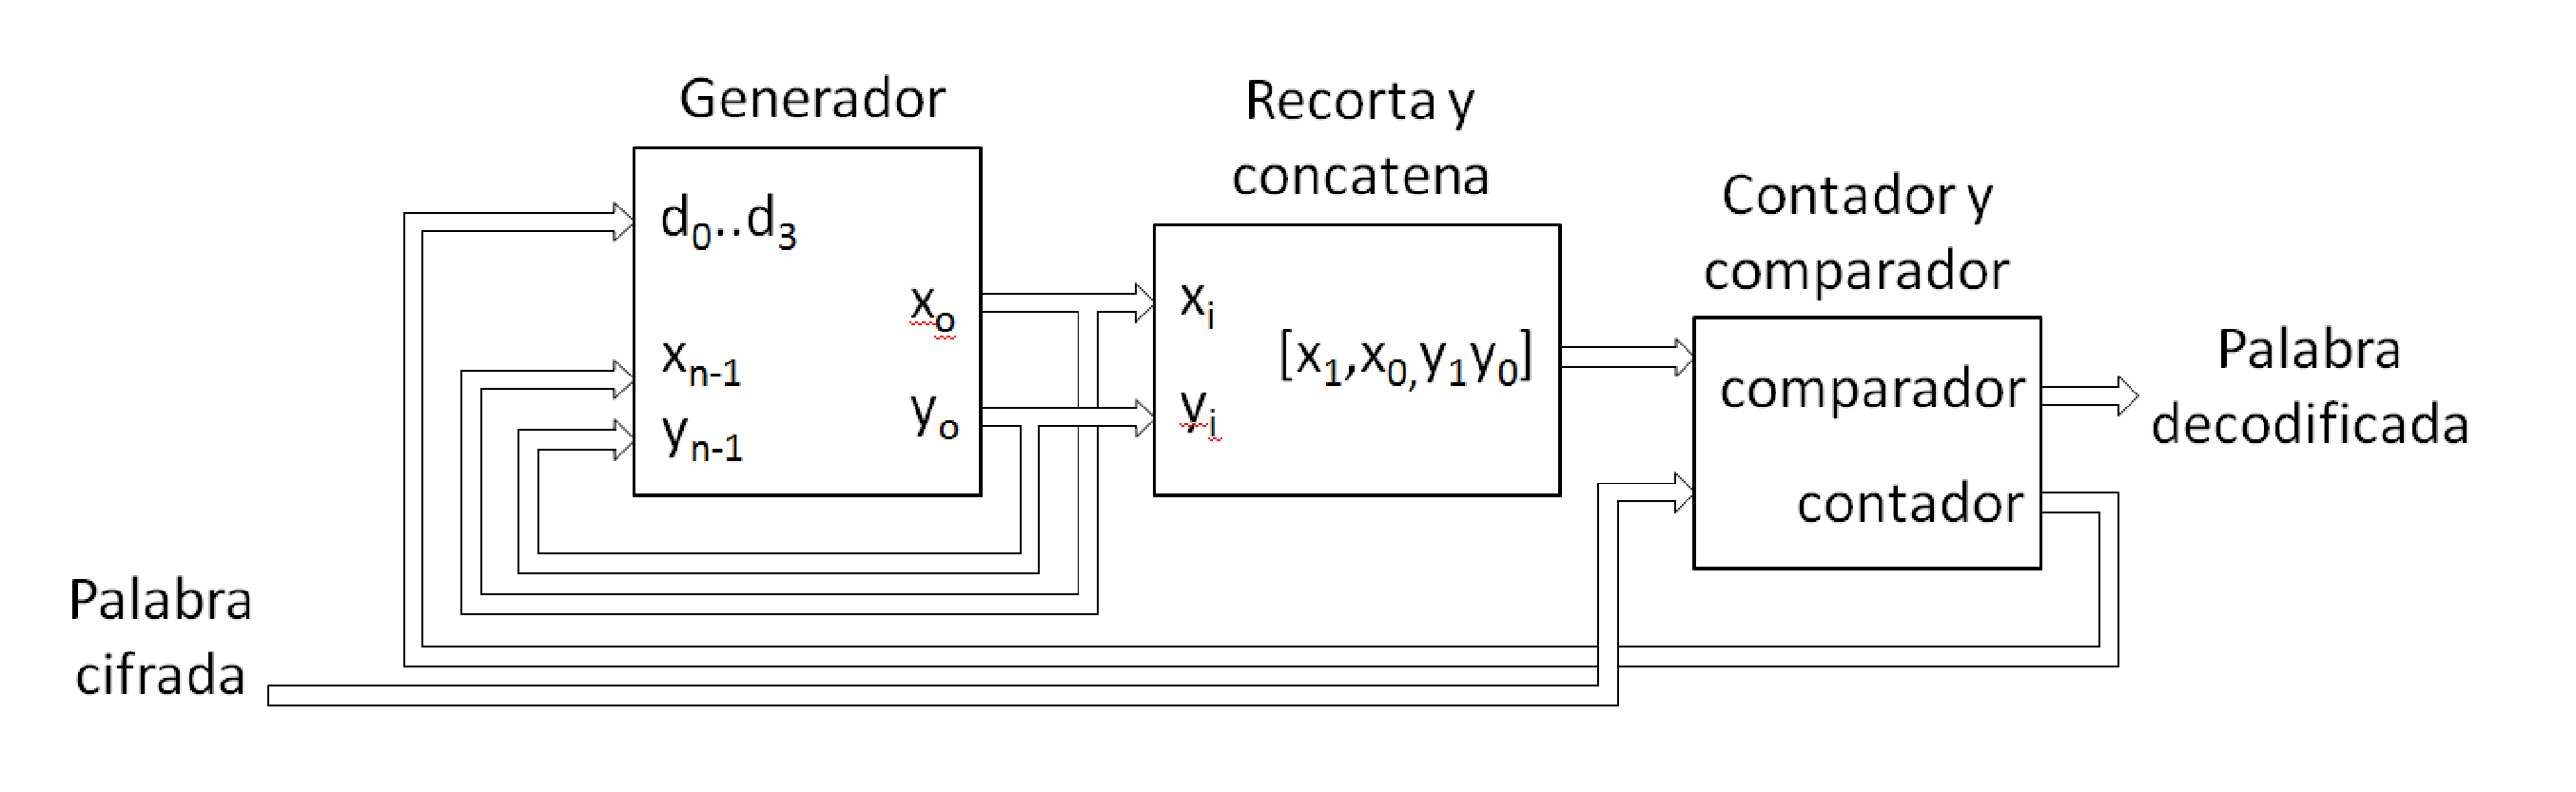
\includegraphics[width=0.8\columnwidth]{Fig3.pdf}\\
    \caption{Decodificador.}\label{fig:decodificador}
\end{figure}

\subsection{Resultados}
Se realizó un primer esquema del diseño mediante la herramienta
Quartus II v8.0 de ALTERA, para implementar el sistema en una FPGA \emph{Altera Cyclone III EP3C120}

Se obtuvieron resultados preliminares de simulaciones realizadas
mediante el programa Matlab y mediante simulaciones con el
programa Quartus de Altera, estas últimas tienen en cuenta el
empelo de la precisión finita elegida para representar los
valores.

En la Fig. \ref{senal} se pueden ver las salidas del bloque
generador para una transmisión de los datos
[1,2,3,2,3,3,1,3,1,3,1]. En este caso se mantiene el dato a enviar
durante $100$ ciclos con el objetivo de que sea visible en la
figura, en el sistema real cada oscilador codifica una palabra de
información en cada iteración. Aqui puede observarse que el
sistema cambia el atractor generado según los coeficientes que
dependen de la entrada de información a transmitir.

En cuanto al análisis de performance que presenta el sistema se
deben tener en cuenta dos aspectos:

\begin{itemize}
    \item
        La distancia mínima de la modulación codificada resultante. Esta  es
        usualmente empleada para proveer un límite de error en la región
        de piso.
    \item
        Una descripción precisa de la tasa binaria de error
        del sistema o BER (en inglés, Bit Error Rate) también es un
        parámetro muy importante, ya que da una estimación del
        comportamiento que presentara el código.
\end{itemize}


\begin{figure}
    \centering
    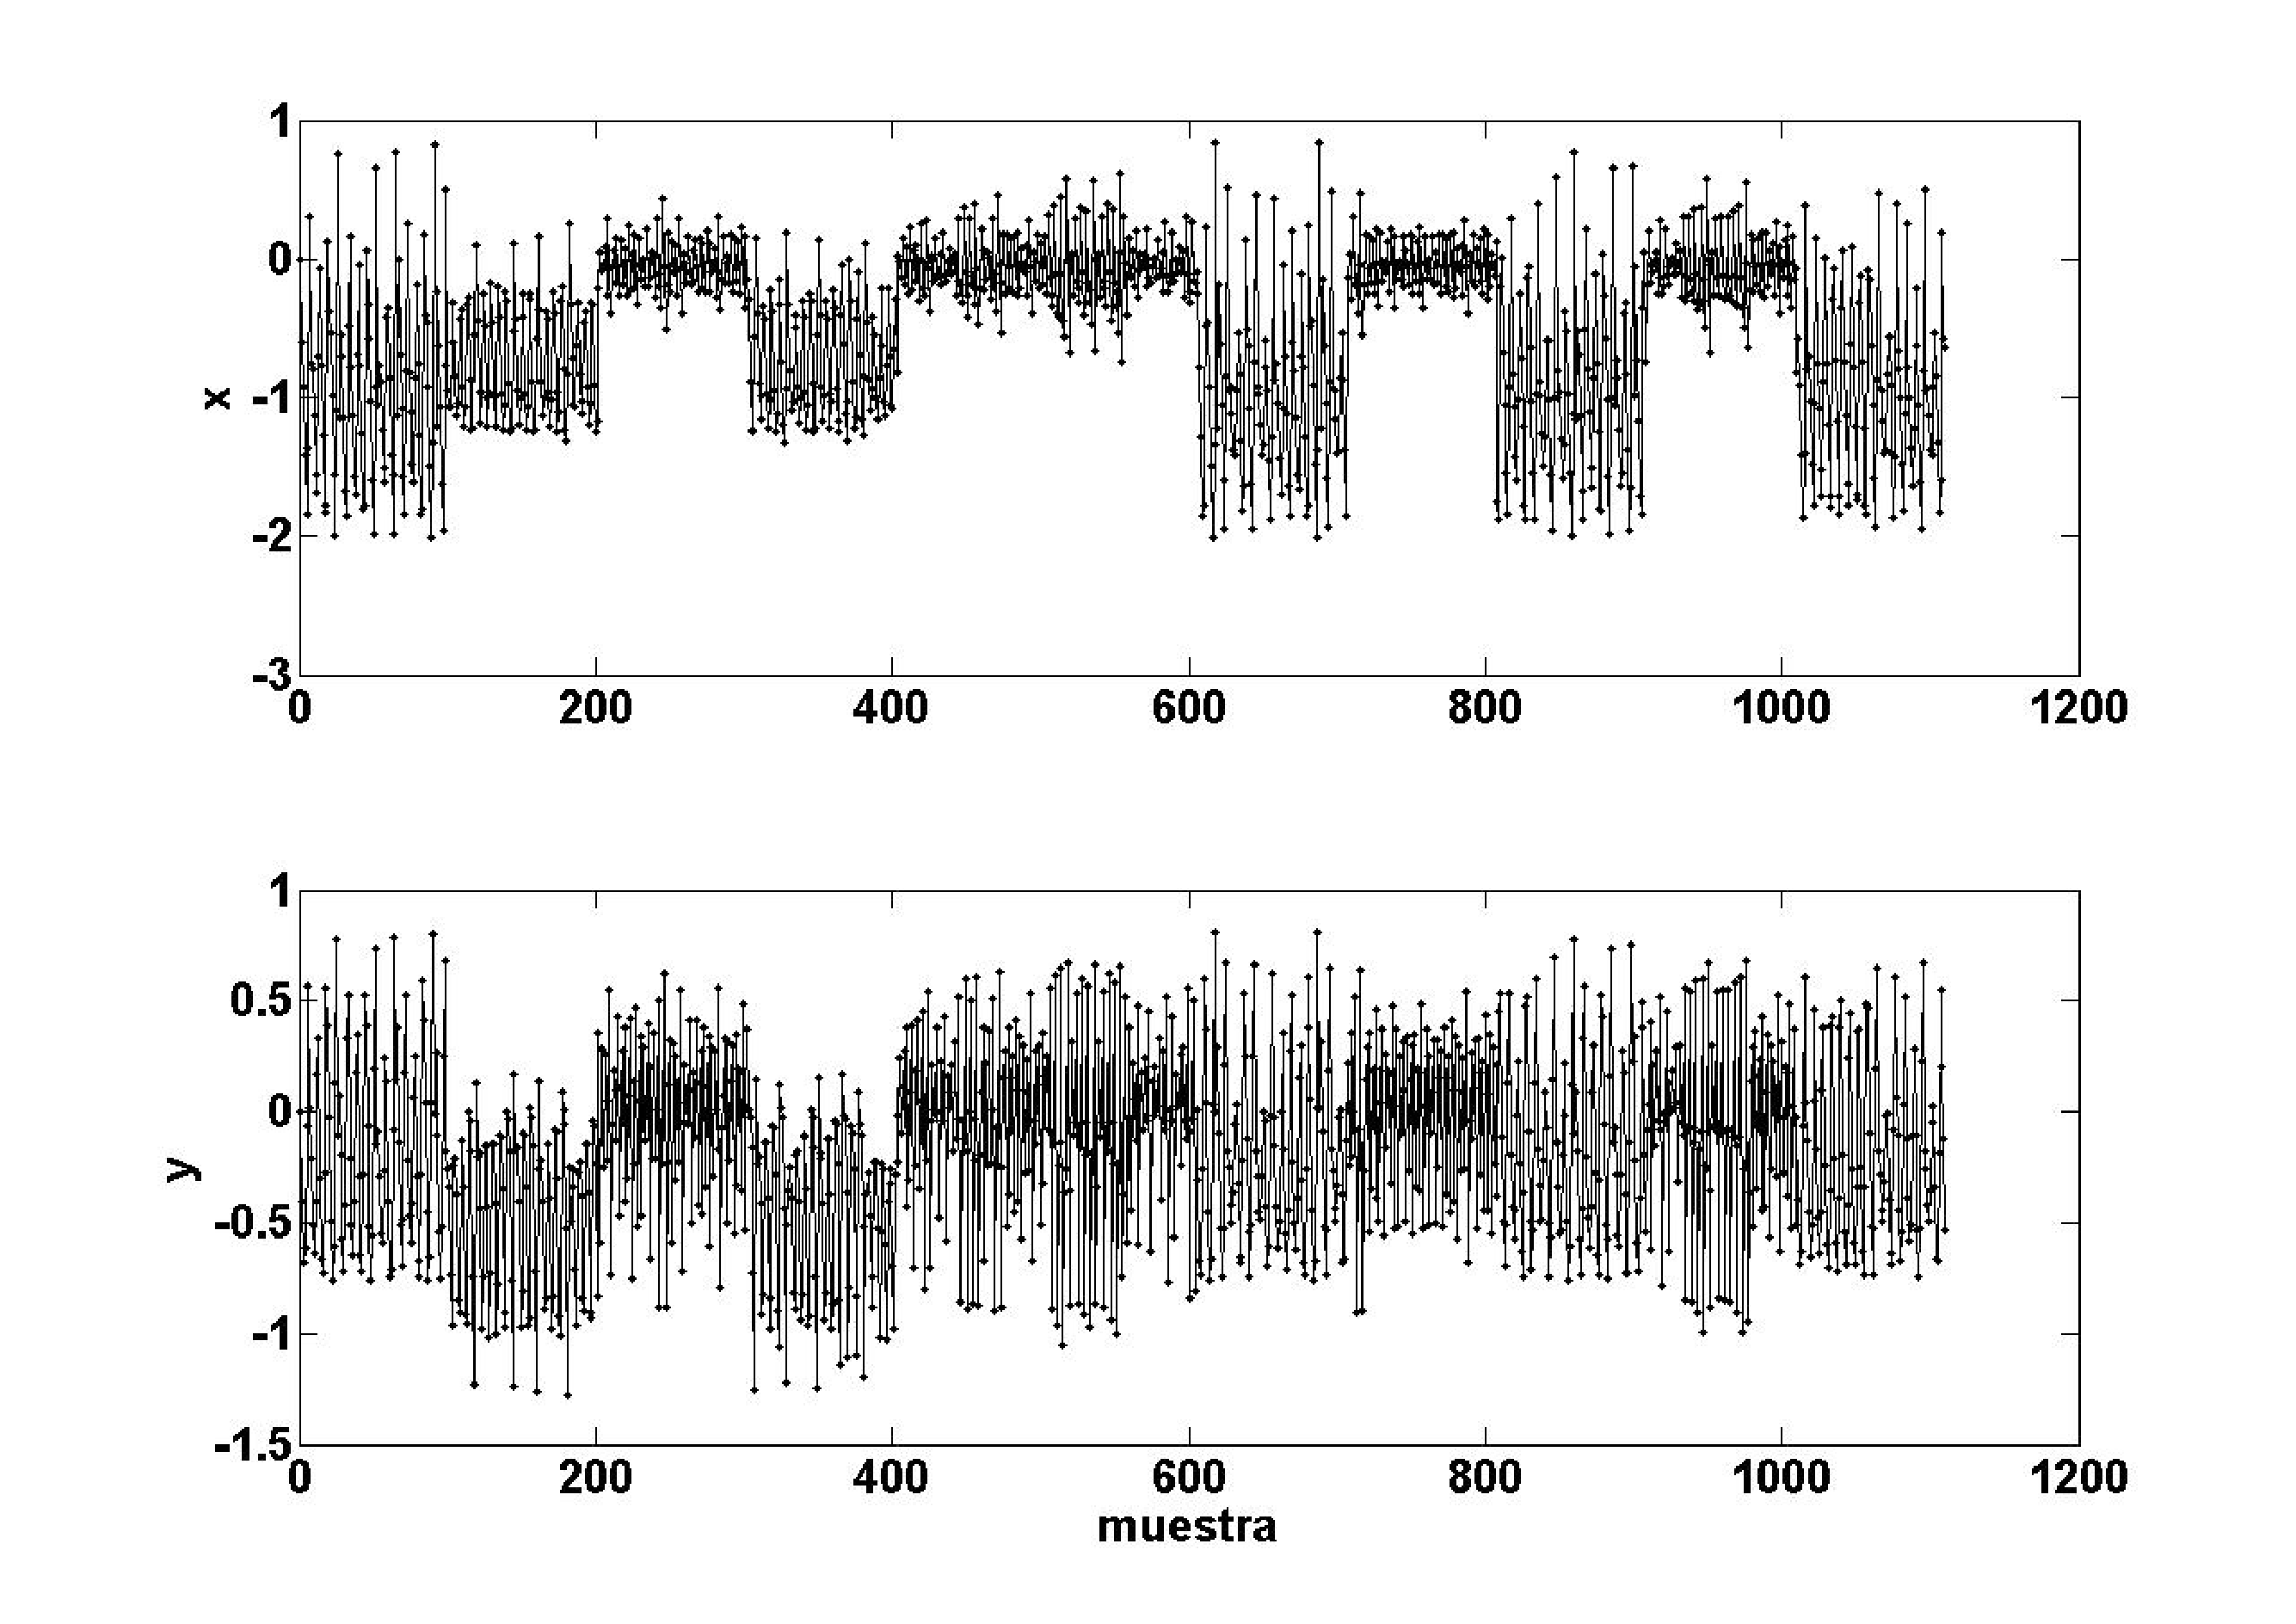
\includegraphics[width=1\columnwidth]{senalent.pdf}\\
    \caption{Señales a transmitir.}\label{senal}
\end{figure}

%\bibliography{xbibWEBjun2012_ingles}

%%%%%%%%%%%%%%%%%%%%%%%%%%%%%%%%%%%%%%%%%%%%%%%%%%%%%%%%%%%%%%%%%%%%%%%%%%%%%%%%%%%%%%%%%%%%

\section{Codificación variable en el tiempo empleando mapa caótico (póster CASE2012)}

Los posters no se si agregarlos o distribuir la información entre los demás capítulos.

En el diseño de un sistema de comunicaciones de datos inalámbrico tanto la confiabilidad de la
transmisión como el nivel de privacía son objetivos a cumplir. Han surgido últimamente técnicas de
codificación que permiten además de aumentar la confiabilidad de la transmisión frente al ruido adicionar
al sistema algún nivel de seguridad. En este trabajo se propone un esquema de codificación que cumple
con ambos objetivos. Este sistema se basa en un mapa cuadrático bidimensional cuya salida presenta un
comportamiento caótico y distintos atractores dependiendo de los coeficientes que se empleen.
Codificar significa básicamente tomar las 2k palabras binarias de k bits que se pretende codificar, y
asignarlas a algunos de los 2n vectores de n bits. Esto se realiza como una función unívoca entre los 2k y
los 2n vectores. Siendo regularmente k < n existen más vectores de n bits que los que se tienen de k bits.
Tradicionalmente el subgrupo de 2n palabras código es fijo y la elección de los vectores de n bits se realiza
empleando la menor redundancia, y maximizando la distancia o separación entre las palabras. En este
trabajo la asignación de los vectores es variable ya que a cada una de las 2k palabras a transmitir se le
asigna un juego de coeficientes que genera salida caótica del mapa. Según la palabra a transmitir el
sistema generará una salida determinada por los coeficientes y el valor inicial, esta será la palabra código
correspondiente a la palabra a enviar. De esta forma, el subespacio de palabras código va cambiando a
medida que la transmisión evoluciona.


%%%%%%%%%%%%%%%%%%%%%%%%%%%%%%%%%%%%%%%%%%%%%%%%%%%%%%%%%%%%%%%%%%%%%%%%%%%%%%%%%%%%%%%%%%%%%%%%%%

\section{Estudio del Caos en Redes Neuronales Discretas para su Implementación en Hardware (Informe Inteligencia computacional, Poster CASE2014)}

Este es bastante largo y completo, pero perdí todos los archivos junto con el disco, tengo el pdf a partir del cual voy a tener que armar el latex de nuevo.

Dentro de los sistemas complejos se encuentran los cóticos, éstos se caracterizan por tener
propiedades estocásticas similares a los de los sistemas aleatorios (en algunos casos mejores),
por ser muy sensibles a las condiciones iniciales y por ser impredecibles a mediano plazo a
pesar de contar con las ecuaciones que describen el sistema. Numerosos trabajos describen el
comportamiento caótico en redes neuronales, este trabajo presenta una detallada descripción
técnica de un caso de estudio.


%%%%%%%%%%%%%%%%%%%%%%%%%%%%%%%%%%%%%%%%%%%%%%%%%%%%%%%%%%%%%%%%%%%%%%%%%%%%%%%%%%%%%%%%%%%%

\section{\emph{RO}-based \emph{PRNG}: \emph{FPGA} implementation and stochastic analysis}

\subsection{Introduction}

The jitter and phase noises present in ring oscillators, are not
convenient in several applications of \emph{RO}s, for example in the implementation of \emph{on-chip oscillators} to generate clocks in high-speed circuits\cite{Hajimiri1999,Mandal2010,Gupta2011}. However they are the source of randomness for \emph{RO}-based \emph{PRNG} \cite{Sunar2007,Wold2009}. Furthermore \emph{RO}s can be implemented in a full-digital circuit like Field Programmable Gate Arrays (\emph{FPGA}s) as they  basically are just a string of inverters.


In \cite{Sunar2007}, Sunar et al. presented a \emph{PRNG} using
stochastic jitter by combining several \emph{RO}s. They required a
post processing of the bit stream, based on resilient functions,
to mask imperfections in the entropy source and to increase
immunity against changes in environmental conditions. The entropy of the bit stream was used to
validate the results in \cite{Sunar2007}.


Wold et al. \cite{Wold2009} proposed an enhanced version with
better random characteristics and without a post processing. They only
added an extra D flip-flop at each ring output. The
effectiveness of their proposal was tested by means of test suites available
in the open literature \cite{NIST2000,marsaglia1995,NIST2000a}.

In this paper a detailed description of a very compact hardware implementation of the \emph{RO}-based \emph{PRNG} proposed in \cite{Wold2009} is done.
In order to validate the randomness of the noise sequences generated, two quantifiers derived from the information theory are used. They define a dual entropy plane $H_{BP}$ vs $H_{hist}$.
$H_{hist}$ is a measure of the first characteristic of a \emph{PRNG} pointed in the abstract, the equiprobability among all possible values. $H_{BP}$ is a measure of the second characteristic pointed in the abstract, the independence between consecutive values. This methodology was successful to evaluate randomizing
techniques applied to chaos-based \emph{PRNG} \cite{DeMicco2008}. A comparison with other options both physical and algorithmic, proposed in the literature is made showing that, in spite of their simplicity, \emph{RO}  are good candidates as \emph{PRNG}.

Organization of the paper is as follows: section \ref{sec:hardware} describes the
hardware implementation of the \emph{RO}s mapped in
\emph{FPGA} Cyclone III. Section \ref{sec:method} shows how the normalized entropies are
determined (to keep this paper short we do not detail already
published results); \ref{sec:results} presents the
results obtained for different configurations of the same
\emph{PRNG}s proposed in \cite{Wold2009}, and the statistical comparison with other utilized \emph{PPRNG}s.
Finally we present our conclusions in Sec. \ref{sec:conclusions}.


\subsection{Hardware implementation.}

The implemented \emph{PRNG}'s consist of  several \emph{RO}s
with their outputs XORed together and sampled by a \emph{D} flip flop,
The flip flop latches the output at a selected frequency (here $100$MHz)\cite{Wold2009}.
The physical implementation is made on \emph{ALTERA}$^{\copyright}$  \emph{Cyclone} III \emph{EP3C120}
development kit with a \emph{EP3C120F780C7N} \emph{FPGA}. The design is made with \emph{Quartus}$^{\copyright}$  II 13.1 software.

\subsubsection{Chip Overview.}

\emph{FPGA}s consist of a large number of logic array blocks (\emph{LAB}s), with groups of logic elements (\emph{LE}s) for implementing sequential as well as
combinatorial circuits. In the \emph{Cyclone} III family architecture
each \emph{LAB} contains $16$ \emph{LE}s.
Basically, each \emph{LE} is a Flip Flop (\emph{FF}) with a
four-input look-up table (\emph{LUT})  (see Fig. \ref{fig:LE}). Each
\emph{LUT} can implement any function of
four variables. The \emph{FF} and the \emph{LUT} can be used together or independently, \cite{Altera}.

%=========================================
 % FIGURA
\begin{figure}
\begin{center}
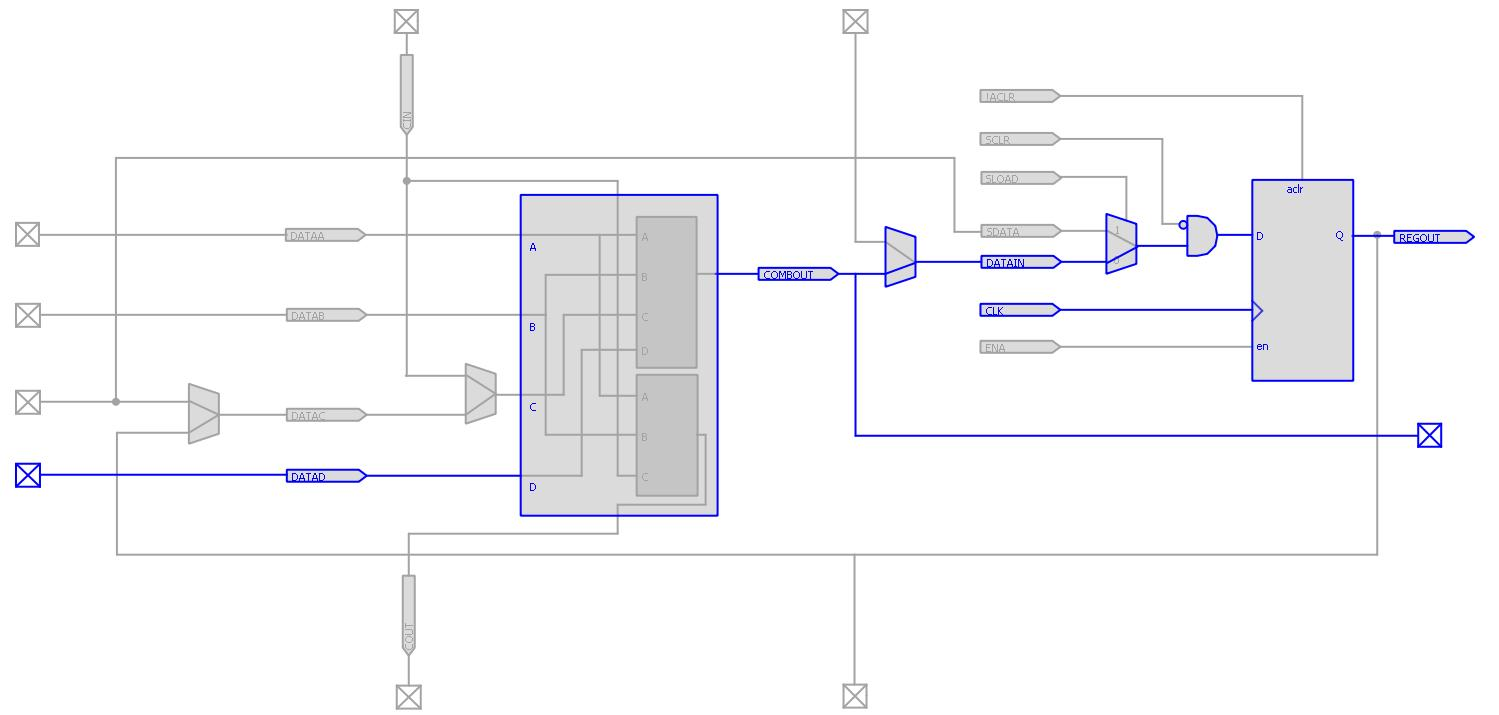
\includegraphics[ width=0.5\textwidth]{NOTenLEmasFF}
\caption{\emph{LE} implementing an inverter and a Flip Flop, Chip Planner
view.} \label{fig:LE}
\end{center}
\end{figure}
%=========================================

Usually, the logic synthesis software assigns \emph{LE}'s
resources without the designer intervention. But in the design of
\emph{RO}-based \emph{PRNG}s it is necessary to control the exact location of
each individual component for two reasons: 1) to avoid the
simplification of the inverters performed by the synthesis tool; 2) to locate
each \emph{RO} in the desired place. In \emph{Altera} the use of low-level primitives enables one to
control the hardware implementation for each \emph{cone of logic} \cite{LowLevel}. Consequently
low-level primitives and assignments are employed inside the \emph{HDL} (hardware description language) code employed in our design.

Strings of \emph{RO}s can be programmed on the chip by
instantiating the \emph{LUT}s as inverters.
In the case of \emph{RO}s it is necessary to prevent the \emph{Quartus} II synthesis engine to merge two \emph{NOT} gates in series, by using a primitive called \emph{LCELL}.
 A \emph{LCELL} always consumes one logic cell and it is not
removed from the project during logic synthesis.

These primitives allow one to break up the design into manageable parts. Each cone is as small as a \emph{LCELL} instantiation.
To create a \emph{RO}, \emph{LCELL}s are programmed as inverter-buffers. Figs. \ref{fig:RTL1ring} and \ref{fig:postMap1ring} show how this primitive is implemented by the Quartus II compiler.

\begin{figure*}
\begin{center}
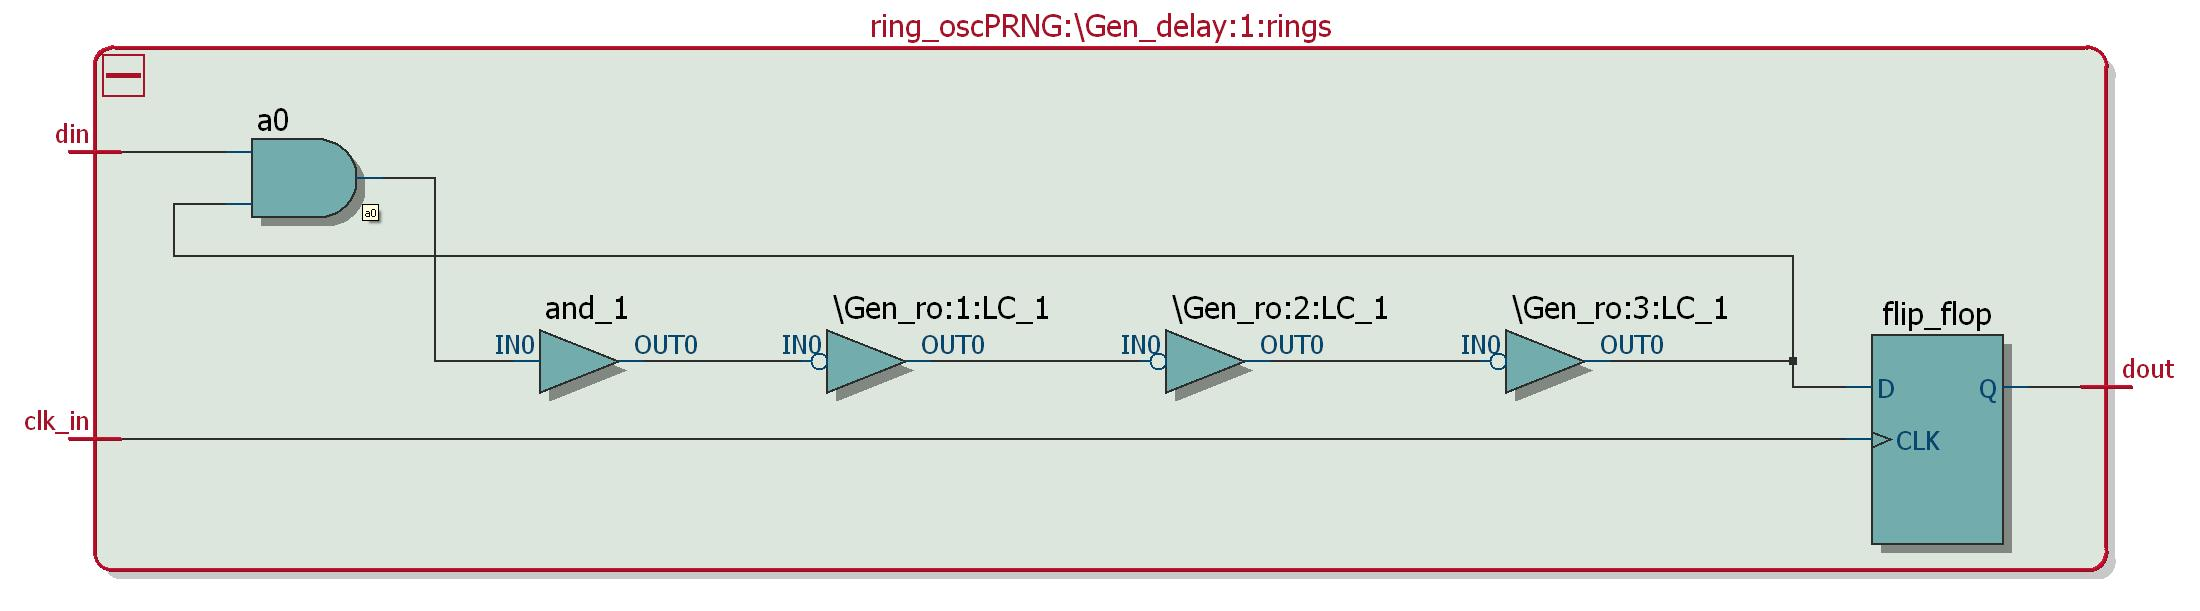
\includegraphics[ width=0.7\textwidth]{RTL_view_1ring}
\caption{RTL view one ring with $3$ inverters.}
\label{fig:RTL1ring}
\end{center}
\end{figure*}

%=========================================
 % FIGURA
\begin{figure*}
\begin{center}
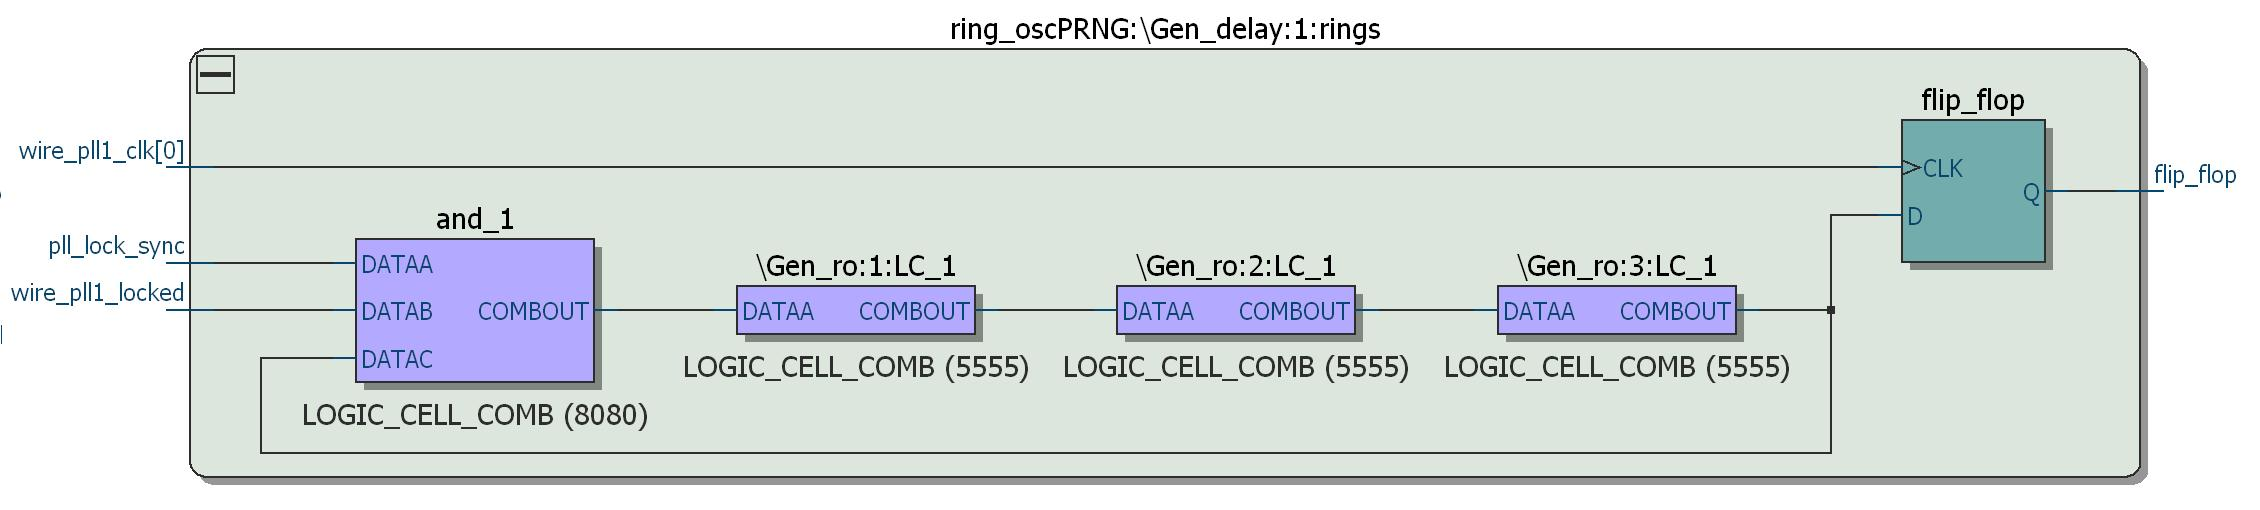
\includegraphics[ width=0.7\textwidth]{tech_map_viewer_post_mapping}
\caption{Technology map viewer (post mapping), one ring with $3$
inverters.} \label{fig:postMap1ring}
\end{center}
\end{figure*}
%=========================================

Furthermore, to avoid the synthesis tool to optimize removing the redundant buffers away,
the \empty{Ignore \emph{LCELL} Buffers} must be set in
\emph{OFF} in the \emph{More Analysis \& Synthesis
Settings} dialog box. Also \emph{Remove Redundant Logic Cells}
must be set to \emph{OFF}.

In order to place each \emph{RO} at a desired position, it
must be assigned to a previously defined \emph{LogicLock region}. In this way the \emph{fitter} will keep all the elements of each ring inside the same region,
\cite{LogicLockRegions}. The process of mapping all the elements to a particular location on the chip
(\emph{LogicLock} region) is achieved by the \emph{Assignment
Editor} tool, that also allows one to verify
that the placements are actually still there, after the  \emph{Synthesis} and \emph{Place \& Route} processes.

Fig. \ref{fig:fpgaplan} shows the $50$ \emph{LogicLock} regions used in this paper as they are
established in the die. One \emph{RO} is assigned to each region.
Regions are spread over the die for a future analysis of location importance. Each region has  $16$ \emph{LAB}s, to allow us to increase the number of inverters of each ring, an issue to be considered in future work.


%=========================================
 % FIGURA
\begin{figure*}
\begin{center}
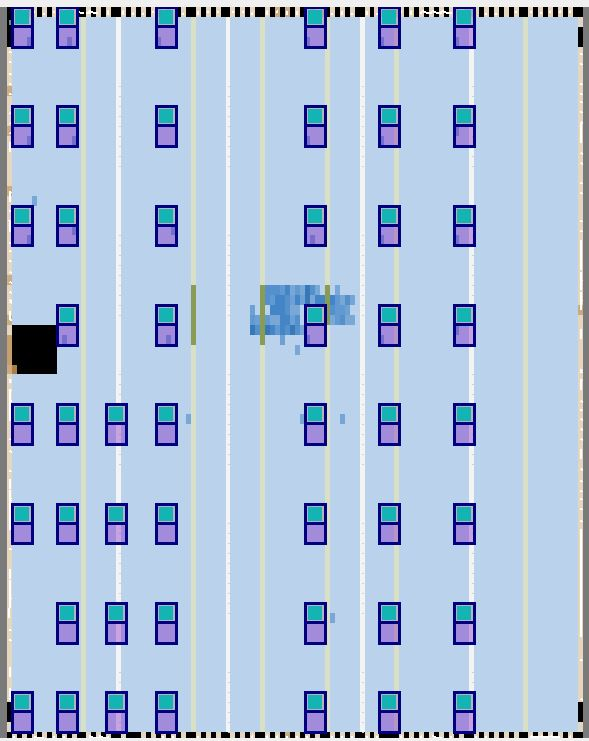
\includegraphics[ width=0.5\textwidth]{fpgaplan}
\caption{\emph{Chip Planner} view \emph{LogicLock} regions.}
\label{fig:fpgaplan}
\end{center}
\end{figure*}
%=========================================

 $3-$inverters, employed in a \emph{RO} and the \emph{FF} were all mapped onto a  \emph{LE} each, meaning that the block
utilization is $4$ of $16$ \emph{LE}s for any \emph{LAB}.


Fig. \ref{fig:LE} displays a single \emph{LE}, there an inverter is
implemented in the \emph{LUT} and it can be seen the exact
\emph{LUT} input that is used. Also the output \emph{FF} of
the ring is mapped there.


There are many factors that determine the frequency of each
\emph{RO}, and contributes to the unpredictability of the output:
\begin{enumerate}
\item Placement within the \emph{LAB}: different placements between rings could result in timing differences.
\item Connections: even having exactly
identical placement of the \emph{LUT}s with respect to each other
in a given ring, it is not possible to have exactly the same
\emph{routing resource usage} in the connections. A small difference in
\emph{routing resource usage} could affect the ring delay.
\item Input selection:  the \emph{fitter} will choose which
\emph{LUT} input is utilized during the routing stage. But the delay through the \emph{LUT}
depends on which of the four inputs is used and consequently the rings could
also have different delays.
\item Neighborhood: even if the design locks down all the placement and routing of a
section  and everything is
physically locked, the timing can change by a few picoseconds
depending on what is placed and routed around the ring.\end{enumerate}
%
In Fig. \ref{fig:RTL3rings} (RTL view) it is shown a \emph{PRNG} using $3$ \emph{RO}s
followed by a XOR gate.

% FIGURA
\begin{figure}
\begin{center}
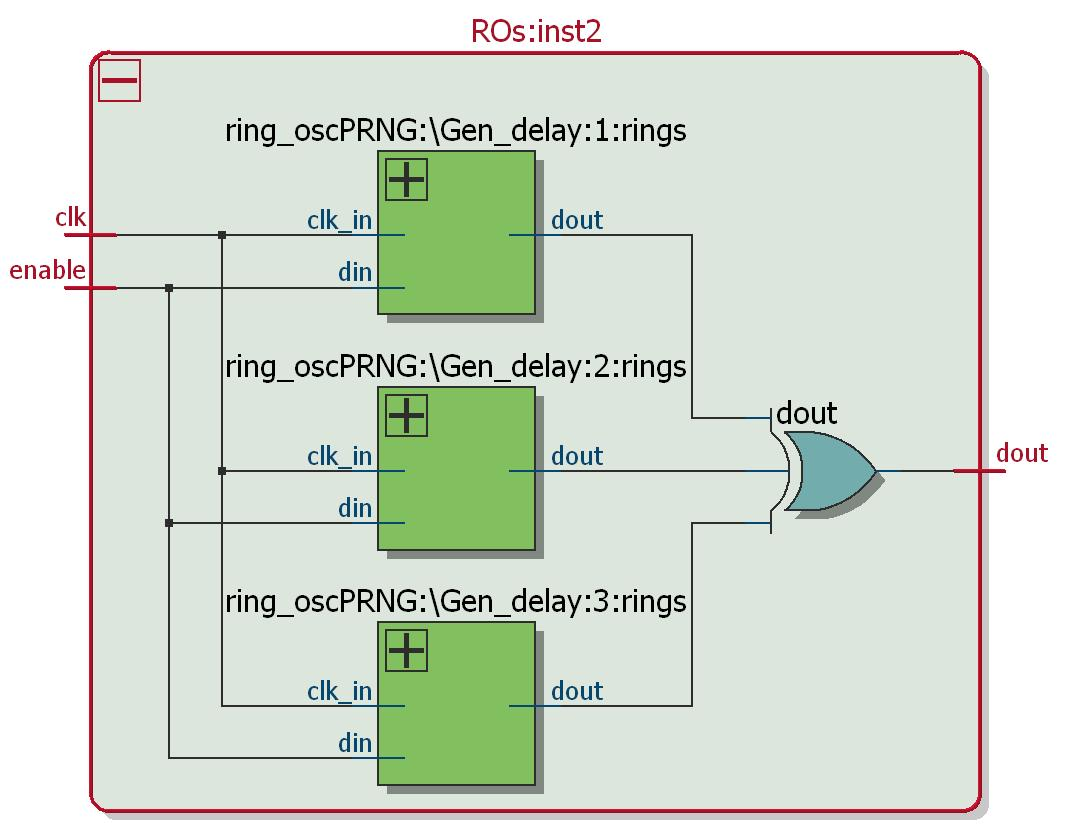
\includegraphics[ width=0.5\textwidth]{RTL_view_3ROs}
\caption{\emph{RTL} view of \emph{PRNG} with $3$ \emph{RO}s.}
\label{fig:RTL3rings}
\end{center}
\end{figure}

%=========================================

Finally, Table \ref{compilation} shows the compilation report of the \emph{PRNG}  using $15$ \emph{RO}s each with $3$ inverters.


%=========================================
\begin{table}
\begin{center}
\begin{tabular}{| l | c  c | }
 \hline
 
\footnotesize{Total logic elements} & $847/119,088$ & $ ( < 1 \%)$\\

 \hline
 
\footnotesize{Total combinational functions} &  $629/119,088$ & $( < 1 \%)$ \\

 \hline
 
\footnotesize{Dedicated logic registers} & $617/119,088$ & $( < 1 \%)$ \\

 \hline
 
\footnotesize{Total registers} &  $617$ &   \\

 \hline
 
\footnotesize{Total memory bits} &  $131,072/3,981,312$ & $( 3 \%)$ \\

 \hline
 
\end{tabular}
\end{center}
\caption{Compilation Report, \emph{RO}-based \emph{PRNG} using $15$ \emph{RO}s and $3$ inverters each.}
\label{compilation}

\end{table}




%==========================================



\subsection{Quantifiers}
\label{sec:method}
Let $X=\{x_i, i=1,...,N\}$ be a length $N$  output of a given
symbolic source with alphabet $\mathcal{A}=\{a_i,i=1,...M\}$. Each
element of $X$ is  $x_i \in \mathcal{A}$. In the case of \emph{RO}
the alphabet is binary consisting of two symbols
$\mathcal{A}=\{0,1\}$. The output is converted into words of $n$
elements. In our case $n=6$. It means we work with a time series
$Y=\{y_i,i=1,...K$ with $K=N/6\}$  of natural numbers $y_i\in [0,2^6-1]$.

The obvious \emph{PDF} (probability density function) to characterize $Y$ is the normalized histogram of the $K$
words $Y$; let us call it  $PDF_{hist}$. Its normalized Shannon
entropy $H_{hist}$ is given by:
\begin{equation}
\label{eq:entropia}
H_{hist}=\frac{\sum_{i=1}^{K}{p_i~log~p_i}}{logK}
\end{equation}

We call this \emph{PDF}  \emph{non-causal} because it does not
change if we permute the time order of the words, and consequently
can not detect any causal connection between consecutive words. The normalized entropy
$H_{hist}$ quantifies the equiprobability of the words among all
possible values. For a \emph{PRNG} its ideal value is
$H_{hist}=1$.

To quantify statistical independence between consecutive words we
use a \emph{causal} \emph{PDF}, proposed by Bandt \& Pompe
\cite{Pompe2002}. This \emph{PDF} is obtained by assigning
ordering patterns to overlapped segments, of length $D$, of the
time series trajectory. The process is as follows: 1) group $D$
consecutive words $\{y_i,y_{i+1},...,y_{i+D}\}$ (let us stress that in our case each
$y_i$ is a natural number $\in[0,63]$). The ordering of the $D$
values inside each group is compared with the order of numbers
$\{1,2,...,D\}$. There exist $D!$ possible permutations of $D$ elements.
Each permutation is called an \emph{ordering pattern}
\cite{Amigo2006} and is labelled with a permutation number
$\pi=1,...,D!$. The normalized histogram of $\pi_i$'s is called
the Bandt \& Pompe \emph{PDF}, $PDF_{BP}$. The normalized Shannon entropy of
this $PDF_{BP}$ is $H_{BP}$ where the subscript $BP$ means ``Bandt
and Pompe".

In case two values of $y_i$ inside the same group are identical,
it is considered that the first one is lower than the last one in
order to obtain an unique result. For \emph{PRNG}s this procedure
does not produce significant changes in  $PDF_{BP}$.

The  Bandt \& Pompe procedure has the advantages of being: 1) simpler and
fast to calculate than block entropies, 2)
robust in presence of noise, and 3) invariant to lineal
monotonous transformations. It is applicable not only to
\emph{PRNG}s but also to any weak stationary process (it means for $k=D$,
the probability that $x_t < x_{t+k}$ does not depend on the
particular $t$ \cite{Pompe2002}). The causality property of $PDF_{BP}$
makes the quantifiers based on this \emph{PDF} to discriminate
between deterministic and stochastic systems \cite{Rosso2007B}.

Bandt and Pompe suggested $3\leq D \leq7$. $D=6$ is adopted
in this work.

A full discussion about the convenience of using different quantifiers
to measure a given \emph{PDF}is out of the scope of this work.
Nevertheless reliable bibliographic sources
do exist \cite{Wackerbauer1994,Lopez1995,Rosso2007A,DeMicco2008,Rosso2009,Martin2006,Rosso2012}.

In this paper we adopt plane $H_{BP}$ vs $H_{hist}$ \cite{DeMicco2008}  to represent each \emph{PRNG}. A higher
value in any of the entropies, $H_{BP}$ and $H_{hist}$, implies an
increase in the uniformity of the involved \emph{PDF}'s. The point
$(1,1)$ represents the ideal point for a \emph{PRNG} with uniform histogram and
uniform distribution of ordering patterns.

\subsection{Results}
\label{sec:results}
%

The  \emph{Embedded Logic Analyzer} tool is utilized for collecting the random sequences generated.
It constitutes a \emph{system-level debugging tool}, provided by $Altera$  \cite{QUARTUS}, that captures and storages the real-time signal behavior and allows one to observe interactions between hardware and software in system designs. After acquiring
the data and  save them into a \emph{SignalTap} II file, they can be
analyzed or viewed as a waveform. With this procedure nor extra jitter neither distortion are introduced in the measured signal from the data acquisition chain.


In the case of \emph{RO} based \emph{PRNG}
data files with $917504$ bits each were generated for each \emph{RO} based \emph{PRNG}.
We consider sets of $N_{RO}$ rings, each with $3$ inverters; $N_{RO}=2$, $3$, $4$, $5$, $6$, $7$, $15$, $25$ and $50$.

Data from $SignalTap$ were  processed using \emph{Matlab}$^\copyright$. Binary data were grouped in $6$-bits words without
superposition, so files with $152917$ data each were generated. Quantifiers described in section \ref{sec:method} were calculated
for all generated files.

We also evaluated other known noises generators to compare their quality with that of  the \emph{RO}-based \emph{PRNG}.
The noises analyzed are:


\begin{itemize}
  \item Mersenne Twister pseudo-random number generator, \cite{Matsumoto1998}.
  \item Two algorithms employed for generate random data by Matlab (Multiplicative Congruential method) \cite{Matlab} and Excel \cite{McLeod1985}.
  \item Two \emph{physical noises}: radioactive decay noise \cite{Walker2001} and atmospheric noise \cite{Haahr}.
  Data files for these noises are available from the referred \emph{websites}.
  \item Two chaotic map $M^1$ and their iterated versions $M^2$ to $M^8$ \cite{DeMicco2008} for the logistic map (\emph{LOGISTIC}) and the \emph{three way Bernoulli map} (\emph{TWBM}).
\end{itemize}

Fig. \ref{fig:HBPvsHhis_all} shows the results in the dual entropy plane $H_{BP}$ vs $H_{hist}$ for all these noises.
It can be seen that the \emph{physical noises}, the algorithmic \emph{Mersenne Twister}, and the \emph{PRNG}s used in \emph{Matlab} $^\copyright$(\emph{rand} function) and \emph{Excel}$^\copyright$ (\emph{RAND} function), have the  maximum value for $H_{BP}$, indicating that all the ordering patterns appear almost the same number of times. However these five noises present very different behavior with respect the $H_{hist}$ quantifier. The \emph{radioactive decay} is the worst, with a value of $H_{hist}$ about $0.5$ indicating that this sequence does not exhibit all possible values in the same proportion. In Fig. \ref{fig:HBPvsHhis_all} the numbers next to each marker for the chaotic sequences, indicate the number of iteration. The iterated maps have higher $H_{BP}$ because of their mixing property \cite{DeMicco2008}.


 % FIGURA
\begin{figure*}
\begin{center}
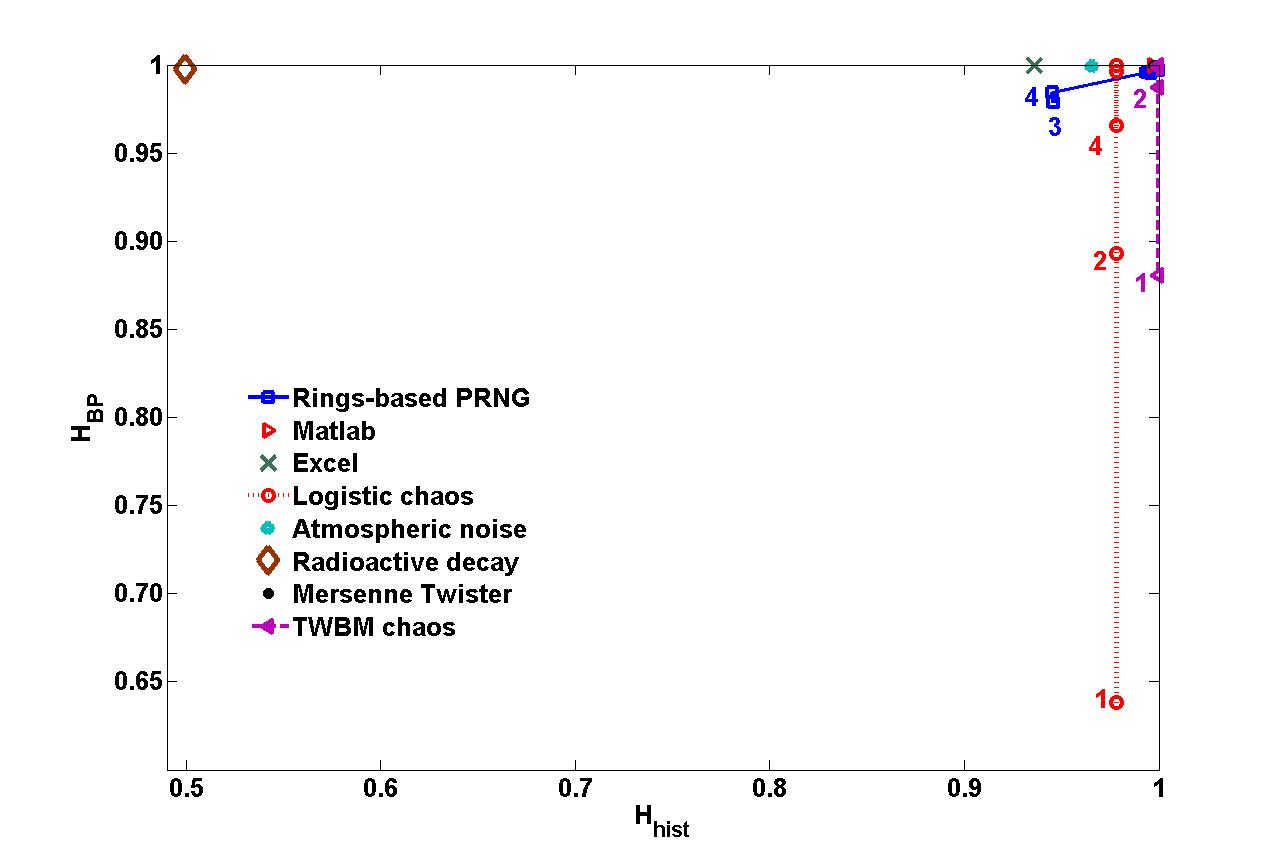
\includegraphics[ width=0.8\textwidth]{HhistvsHBP_t}
\caption{$H_{BP}$ vs $H_{hist}$ plane for several noises, numbers next to each square indicate the quantity of \emph{RO}s
used in the \emph{RO} based \emph{PRNG}. Numbers next to each point in the  chaotic sequences labeled \emph{Logistic}
and \emph{TWBM} indicate the number of iteration of the chaotic map (see the text for details).}
\label{fig:HBPvsHhis_all}
\end{center}
\end{figure*}
%=========================================

In the case of the \emph{RO}-based \emph{PRNG} sequences, numbers next to each square indicate the quantity of \emph{RO}s employed in that \emph{PRNG} (let us stress that the number of inverters is fixed to $3$). The dual entropy plane shows that  an increase in the number of \emph{RO}s improves both $H_{BP}$ and $H_{hist}$.

Fig. \ref{HhistvsHBP_zoom} is a zoom of Fig. \ref{fig:HBPvsHhis_all}  around the ideal point $(1,1)$.


%=========================================
 % FIGURA
\begin{figure*}
\begin{center}
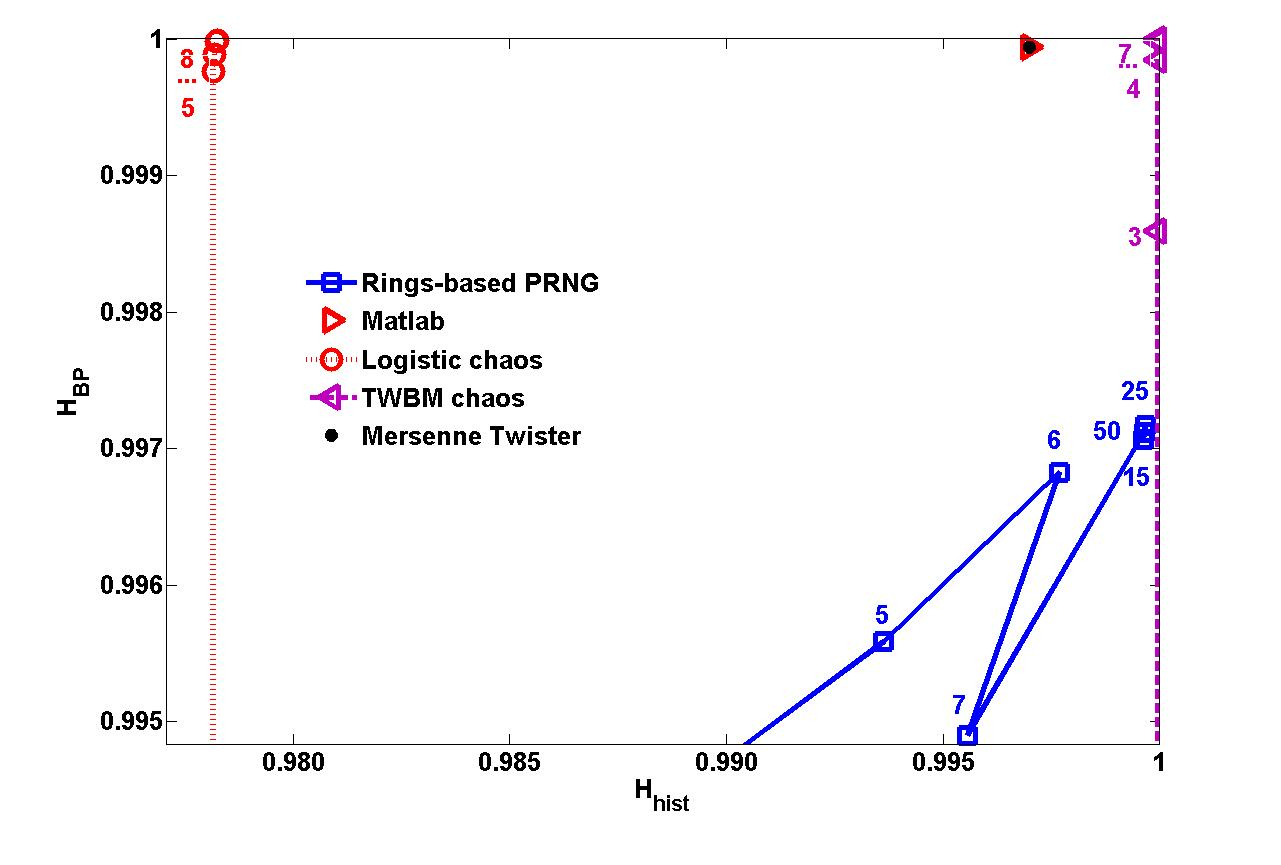
\includegraphics[ width=0.8\textwidth]{HhistvsHBP_z}
\caption{Zoom of Fig. \ref{fig:HBPvsHhis_all}  around the ideal point $(1,1)$ of the $H_{BP}$ vs $H_{hist}$ plane. Numbers next to each square indicate the number of \emph{RO}s used in that rings-based \emph{PRNG}. Numbers next to each point in the chaotic sequences indicate the number of iteration of the chaotic map.} \label{HhistvsHBP_zoom}
\end{center}
\end{figure*}
%=========================================

There, it is shown the evolution of the \emph{RO}-based \emph{PRNG} sequences when the quantity of \emph{RO}s increases from $5$ to $50$ (numbers next to each square). It can be seen that as the number of rings increases, data increase their mixture and also the histogram tends to be more uniform. So both properties are improved. Here a threshold in the number of rings can be determined, as the points saturate at about $(0.997,1)$, so this is the best \emph{PRNG} possible. Further, using more than $15$ \emph{RO}s presents no improvement.
As it was previously said, $H_{hist}$ quantifier detects the histogram variation of the sequence, and the $H_{BP}$ quantifier reflects the improvement in the mixing of data.
Finally, Mersenne Twister and Matlab sequences present identical value, ideal $H_{BP}$, and a high value of $H_{hist}$ nonetheless the histogram is not perfectly uniform (values are not equiprobable).

\subsection{Conclusions}
\label{sec:conclusions}
\emph{RO}-based \emph{PRNG} implemented here has demonstrated to satisfactorily meet the statistical properties desired by a \emph{PRNG}. They are comparable of other used \emph{PRNG}s and in some cases they are better. They employs few resources of the device and they are simply to implement in a digital platform.

It was demonstrated that for these architectures of \emph{PRNG} the quantity of
\emph{RO}s establishes \emph{PRNG}'s statistical properties. It was seen that
for $15$ \emph{RO}s both output's statistical properties, histogram
and mixing, were almost ideal, making unnecessary the increase of the number of rings.

The dual entropy plane proposed here has demonstrated to satisfactorily discern between the \emph{PRNG}'s two main desired properties, the equiprobability among all possible values and the statistical independence between consecutive values. Thus, it allows to clearly see what needs to be improved in a given sequence.



%\bibliographystyle{IEEEtran}
%\bibliography{xbibwebjulio2014_ingles,xbibMAXI_300314}  %


%%%%%%%%%%%%%%%%%%%%%%%%%%%%%%%%%%%%%%%%%%%%%%%%%%%%%%%%%%%%%%%%%%%%%%%%%%%%%%%%%%%%%%%%%%%%%%%%%

\section{Implementación de algoritmo genético para la búsqueda automática de caos en sistemas multiatractores (póster CASE2013)}

Se generó una lógica basada en algoritmos genéticos encargada de evolucionar los
parámetros del sistema de modo que cada generación tenga un comportamiento
caótico mejor que la anterior [3]. El target (fitness function), por lo tanto, es el MLE.
Para mayor claridad se separó el diagrama de flujo en dos partes, un diagrama principal
y una subrutina.
El sistema se inicializa en un conjunto de coeficientes llamado población inicial,
semilla o padre y se calcula su fitness function (Fp). Luego, se genera un incremento de
estos parámetros generando un hijo, que ingresa a la subrutina Evolution que lo
devuelve evolucionado y calcula su fitness function (Fc) para compararla con la de sus
padres. Las posibilidades son tres: el hijo es un padre de la siguiente generación
reemplazando al padre o no, o el hijo es descartado.
La subrutina Evolution es un algoritmo muy simple basado en mutaciones. Se
varían ligeramente los coeficientes del sistema (generando mutaciones) evaluando su
fitness function (Fm) buscando un máximo local.

\thispagestyle{empty}

\chapter{Cuantificadores de Aleatoriedad}

\section{Máximo Exponente de Lyapunov}
\label{sec:MLE}

El Máximo Exponente de Lyapunov (MLE) caracteriza que tan rápido se apartan dos trayectorias.
Si esta velocidad es exponencial, se dice que el sistema es caótico, por lo que este exponente es conocido como un detector de  ``caoticidad", \cite{strotgartz1994,Kantz1994,Sprott2003}.
Más adelante, el MLE fue utilizado en diversas aplicaciones de muy distintas áreas.
Sólo por mencionar alguna, en \cite{Ma2013} el MLE es usado para medir una señal muy débil en un gas ideal utilizando criterios caóticos.
En \cite{Bruijna2011}, se estudia si es posible predecir un cambio en la probabilidad de caída para un modelo simple de caminante humano a partir del $MLE$.

Los exponentes de Lyapunov son quantificadores que caracterizan como evoluciona la separación entre dos trayectorias \cite{Sprott2003}.
En general es bien conocido que el comportamiento caótico está principalmente caracterizado por los números de Lyapunov de la dinamica del sistema.
Si uno o mas números de Lyapunov es mayor que cero, entonces el sistema se comporta caóticamente, de otra forma el sistema es estable.

La distancia entre dos trayectorias cambia en $2^{MLE}$ por cada iteración, en promedio.
Si el $MLE<0$ las trayectorias se aproximan, esto puede deberse a un punto fijo.
Si el $MLE=0$ las trayectorias mantienen su distancia, esto puede deberse a un ciclo límite.
Si el $MLE>0$ la distancia entre las trayectorias es creciente, lo que es un indicador de caos.

Existe una forma no analítica de medir el $MLE$ si solo las entradas y las salidas de un sistema son accesibles.
El procedimiento es el siguiente: el sistema debe ser iniciado desde dos puntos cercanos en el plano de fase, llamémoslos $(x_a,y_a)$ y $(x_b,y_b)$.
A medida que el sistema es iterado se mide la distancia euclideana entre las dos trayectorias ($d_n$ en la muestra $n_{th}$) (eq. \ref{eq:D0D1}), y la trayectoria $b$ es relocalizada en cada iteración (eq. \ref{eq:reubicacion}) obteniendo los puntos $(x_{br},y_{br})$ para realimentar el sistema.
Entonces, el MLE puede ser calculado como se muestra en la ecuación \ref{eq:Lyapunov}.
El proceso puede verse en la Fig. \ref{fig:relocalizacion}.

\begin{eqnarray}\label{eq:D0D1}
d_{0(i-1)}&=& \sqrt{(x_{a(i-1)}-x_{br(i-1)})^2+(y_{a(i-1)}-y_{br(i-1)})^2}\nonumber\\
d_{1(i)}&=& \sqrt{(x_{a(i)}-x_{b(i)})^2+(y_{a(i)}-y_{b(i)})^2}\\
\nonumber
\end{eqnarray}

\begin{eqnarray}\label{eq:Lyapunov}
MLE &=& \frac{1}{n} \sum_{i=2}^{n} \log_2{\frac{d_{1(i)}}{d_{0(i-1)}}}
\end{eqnarray}

\begin{eqnarray}\label{eq:reubicacion}
x_{br(i)}&=& x_{a(i)}+(x_{b(i)}-x_{a(i)})d_{o(i-1)}/d_{1(i)} \nonumber\\
y_{br(i)}&=& y_{a(i)}+(y_{b(i)}-y_{a(i)})d_{o(i-1)}/d_{1(i)}
\end{eqnarray}

\begin{figure}
	\centering
	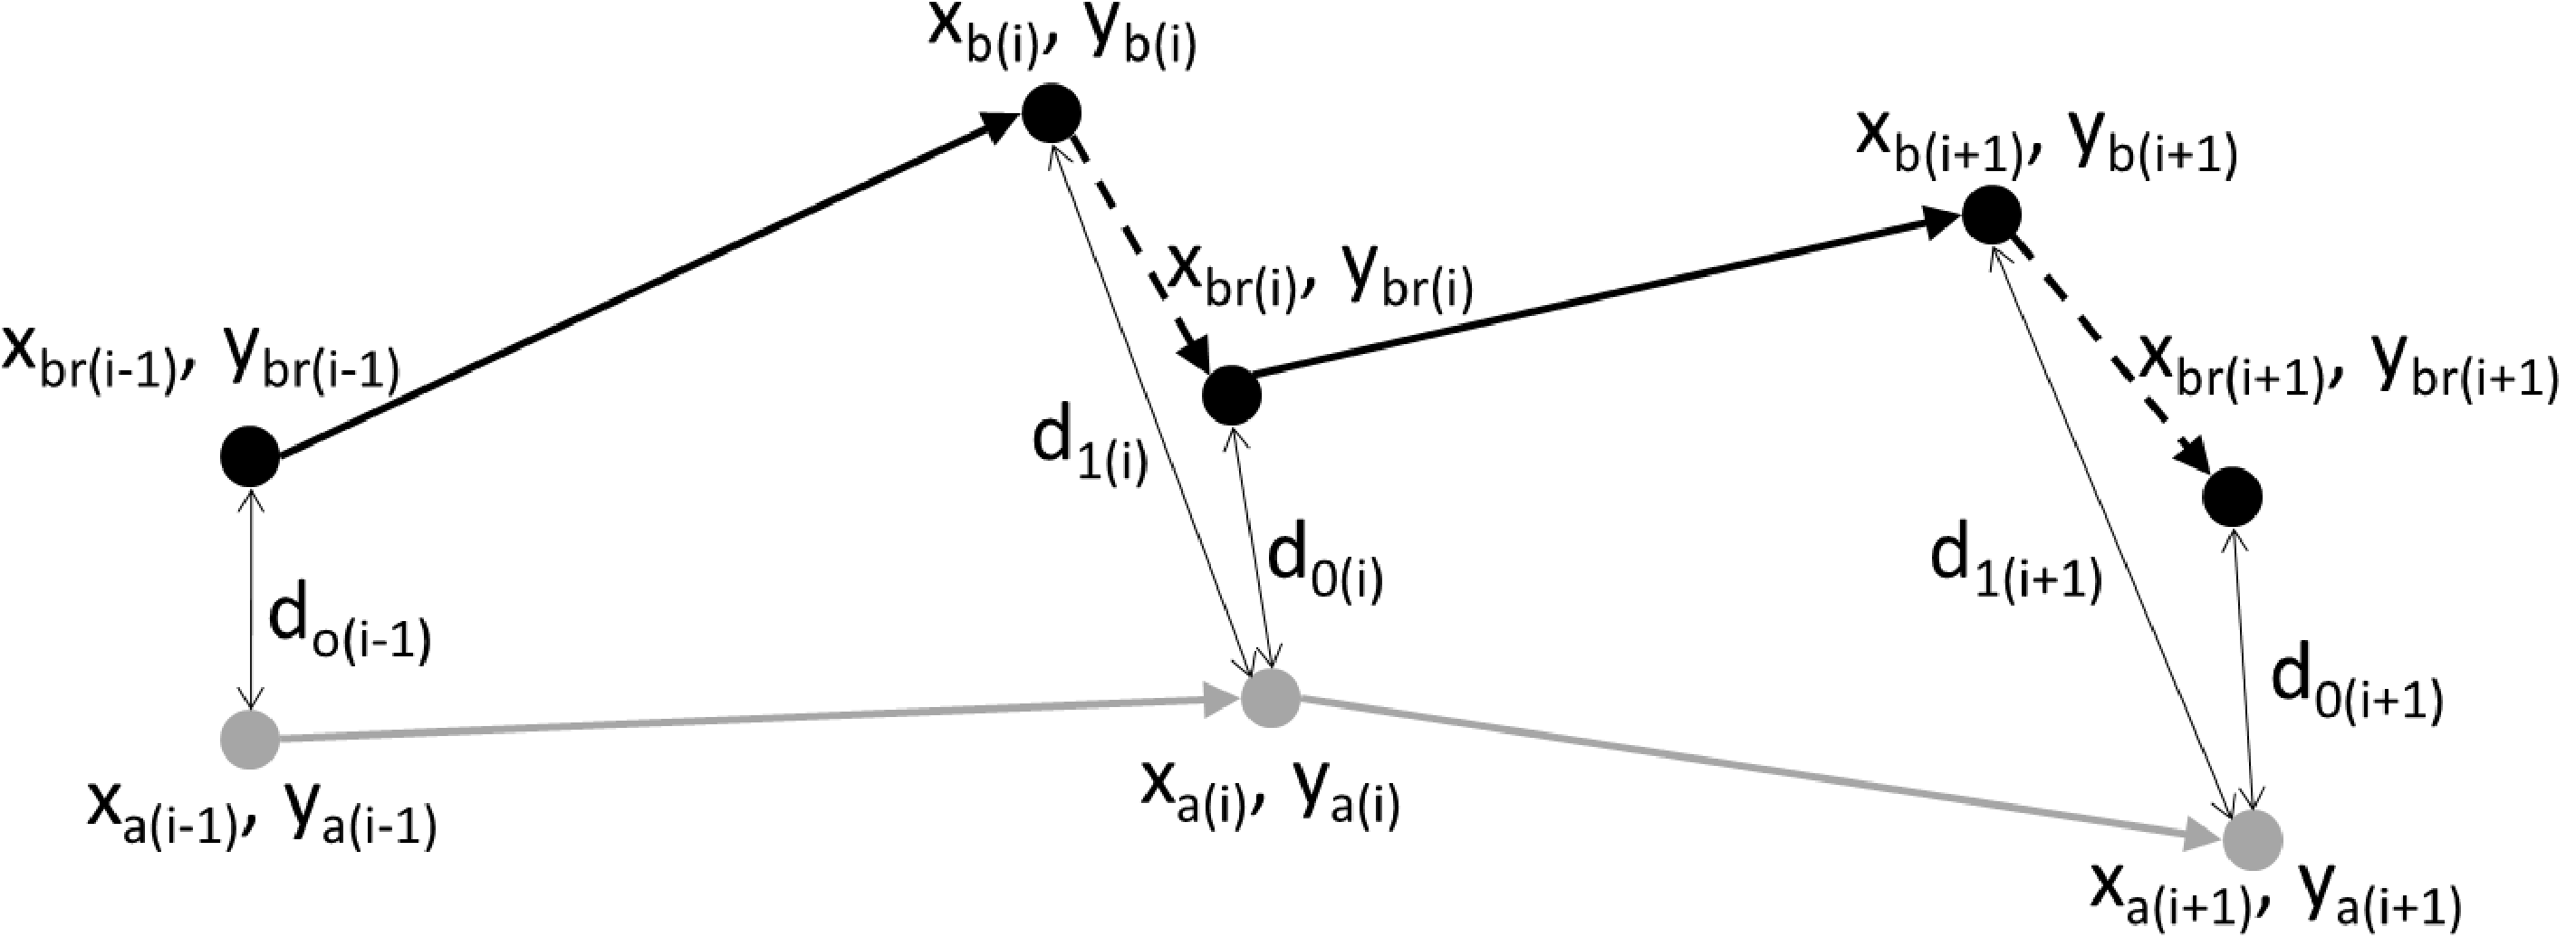
\includegraphics[width=1\columnwidth]{relocalizacion.pdf}\\
	\caption{Algoritmo para calcular el MLE.}\label{fig:relocalizacion}
\end{figure}


\subsection{Algoritmo evolutivo para la búsqueda de caos}

Se propuso emplear un método eurístico para buscar parámetros del sistema implementado de tal forma que se maximice la caoticidad de su salida.
Este algoritmo tiene la ventaja que realiza una búsqueda inteligente mediante el empleo de un algoritmo genético, lo que minimiza el tiempo de cómputo.

Un algoritmo evolutivo es un método de búsqueda dirigido basado en la probabilidad.
Un juego de entidades que representan posibles soluciones compite con otros, evolucionando en mejores soluciones \cite{Weise2009}.

Las entidades que representan posibles soluciones al problema son llamados \textit{cromosomas} y el grupo de cromosomas es llamados \textit{población inicial}.

Desde la población inicial, o los primeros padres, se genera un hijo mediante el cruce entre ellos.
Luego, ellos son mutados en forma aleatoria para crear la próxima generación.
Cada generación es comparada con la previa para descartar los ``peor adaptados" y así los coeficientes (cromosomas) mutan hacia los ``mejor adaptados".

Cuando se aplican estos algoritmos en funciones continuas, siempre convergen hacia el máximo local.
Sin embargo, si el espacio de coeficientes es fractal, existen áreas bien definidas en donde el la función objetivo es positiva, negativa, cero o no existente.
Este es el caso si la función a maximizar es el MLE y el espacio de exploración es el de parámetros.

\subsubsection{Resultados}

Para evaluar la viabilidad del método, se generó el siguiente algoritmo y se probó sobre el mapa logístico.

En la figura \ref{fig:diagramaflujo1} podemos ver el diagrama de flujo principal.
El bloque \textit{Evolution} fue descompuesto en otro sub-diagrama para simplificar la descripción.
Este segundo diagrama puede verse en la figura \ref{fig:diagramaflujo2}, esta surutina maneja la evolución de los parámetros.
%
\begin{figure}
	\centering
	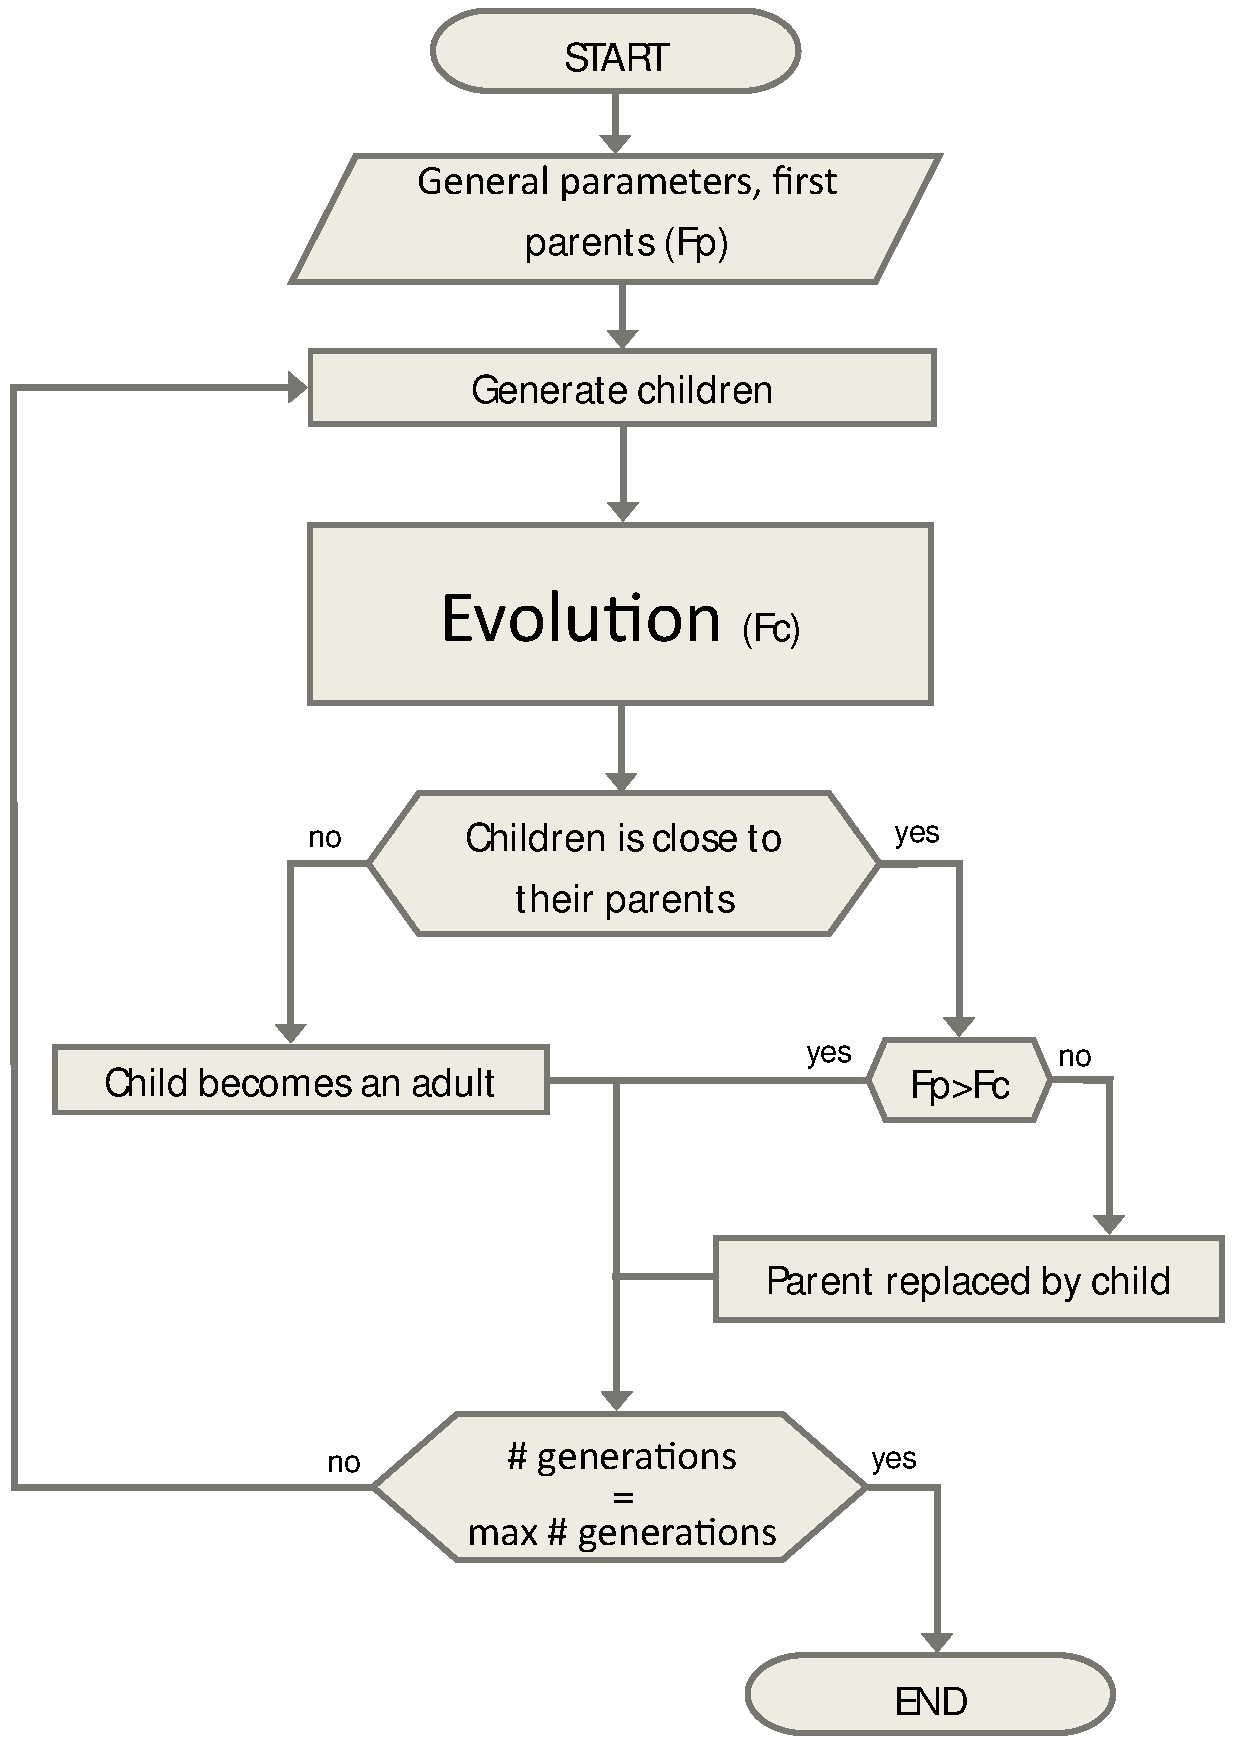
\includegraphics[width=0.9\columnwidth]{main_flowchart}\\
	\caption{Diagrama de flujo principal.}
	\label{fig:diagramaflujo1}
\end{figure}
%
\begin{figure}
	\centering
	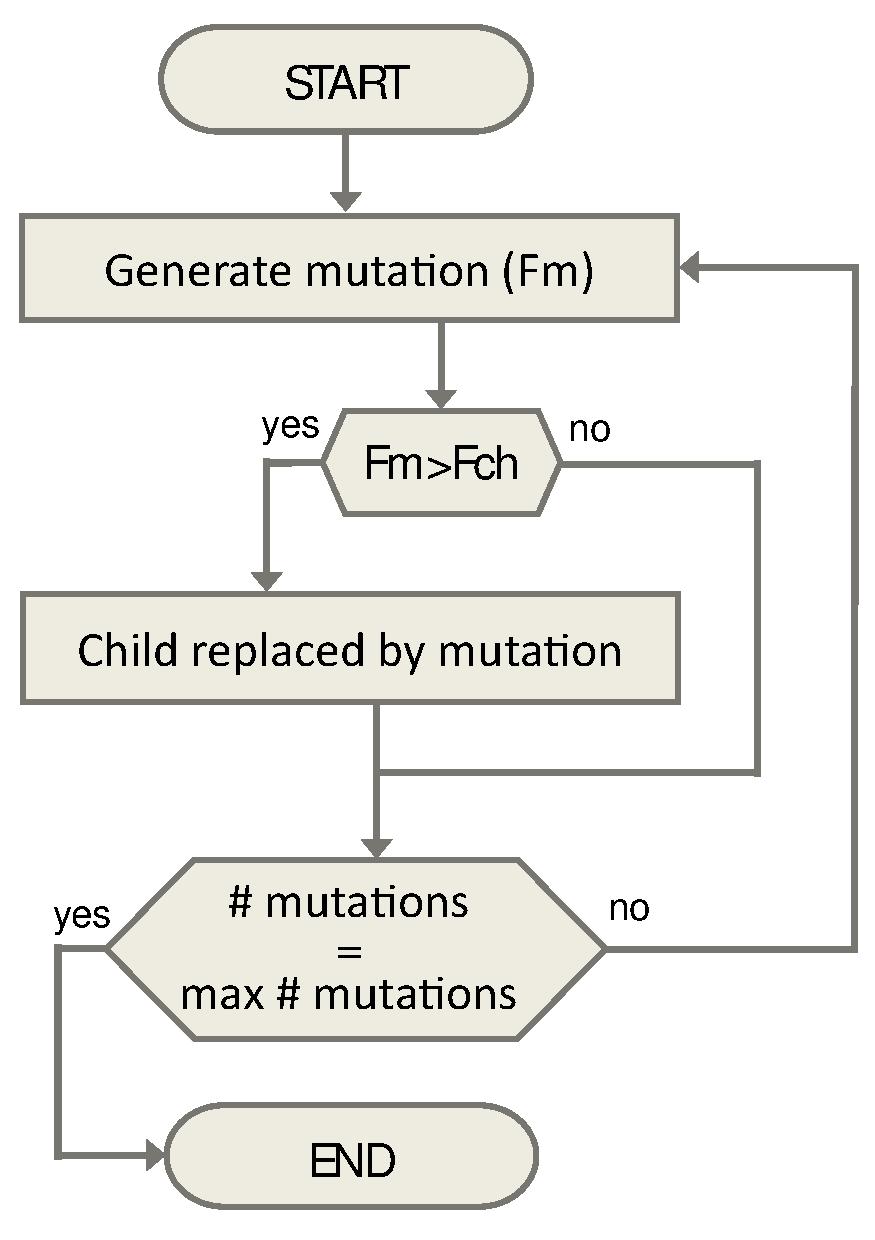
\includegraphics[width=0.56\columnwidth]{evolution_flowchart.pdf}\\
	\caption{Diagrama de flujo del bloque \textit{Evolution}.}\label{fig:diagramaflujo2}
\end{figure}

El algoritmo inicia con una inicialización general de parámetros como el número máximo de generaciones $max\_gen$, el número máximo de mutaciones $max\_mut$ y el número máximo de cambios en cada mutación $max\_stem$.
Luego se definen los primeros dos padres, ellos definirán los márgenes de búsqueda.
Además se calcula su \textit{fitness function} $Fp$.
A partir de este punto se itera la segunda generación, se elige en forma aleatoria un valor de parámetro $r$ con una distribución aleatoria entre los primeros dos padres, generando un nuevo hijo.
Luego este hijo entra en la subrutina \textit{Evolution} cuya salida es el valor de $r$ evolucionado y su correspondiente $Fc$.

Luego se evalúa si este hijo avolucionó muy cerca de sus padres o no.
Si la distancia entre ellos es más grande que el parámetro $max\_hop$, entonces este hijo es considerado como adulto, en caso contrario debe competir con su padre más cercano sobreviviendo el más apto.

Este proceso se repite hasta que se llega al máximo número de  generaciones $max\_gen$.
El grupo final de adultos es la solución al problema de buscar los máximos MLE locales.

La subrutina \textit{Evolution} de la figura \ref{fig:diagramaflujo2}) es un algoritmo muy simple basado en mutaciones.
El primer paso es generar una mutación del hijo con una probabilidad uniformemente distribuida entre $\pm max\_step$, tambien se calcula su \textit{fitness function} $Fm$, que se compara con la del individuo original $Fc$.
Entonces sobrevive el mejor adaptado para dar lugar a la siguiente mutación.
Este procedimiento se repute hasta que se llega al máximo número de mutaciones $max\_mut$.

Como resultado podemos ver el $MLE$ del mapa logístico en función de su único parámetro $r$ en la figura \ref{fig:resultadoAlgorithm}.
La línea contínua muestra el $MLE$ en pasos continuos de $r$, mientras que los puntos destacados son el resultado del algoritmo propuesto.
%
\begin{figure}
	\centering
	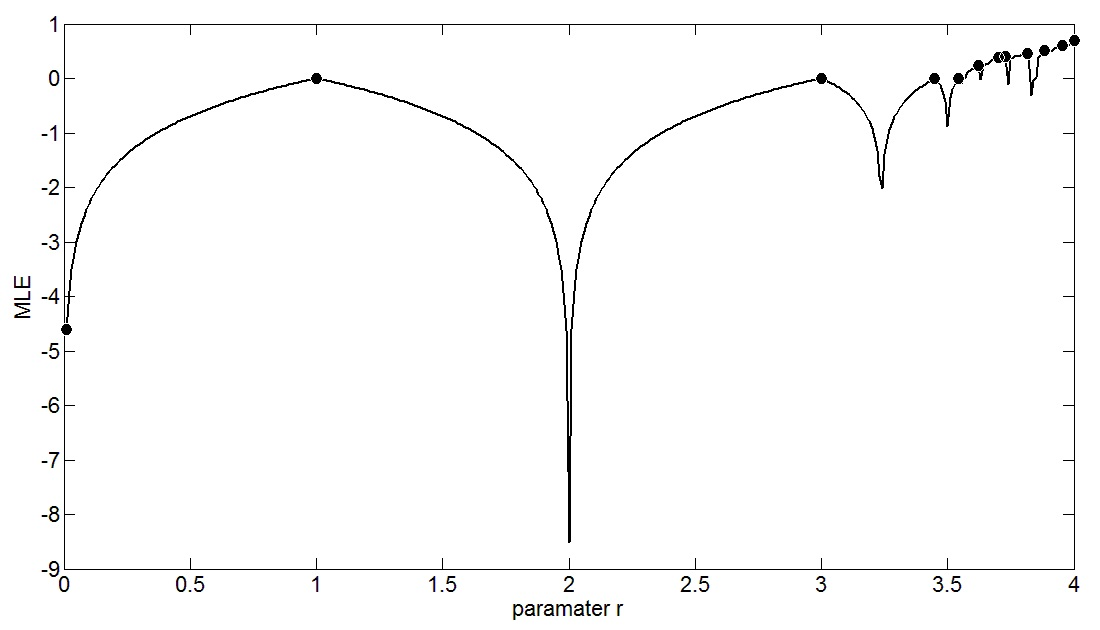
\includegraphics[width=1\columnwidth]{EvolutivoVSExaustivo.jpg}\\
	\caption{Resultados del algoritmo evolutivo para el mapa logístico, los puntos son los resultados del algoritmo.}\label{fig:resultadoAlgorithm}
\end{figure}

El bloque que calcula el $MLE$ fue sintetizado y verificado experimentalmente en un Altera CYCLONE III FPGA y los resultados de la compilación mostrados en la figura \ref{fig:compilacion}.
Los resultados del \textit{Timing Analysis} reportan que la máxima frecuancia es de $84.95MHz$.
El reporte de compilación muestra que la utilización de la lógica no excede el $20\%$, es decir un total de $20307$ de elementos lógicos, $54\%$ de los bits de memoria totales y $8\%$ de los multiplicadores embebidos.
%
\begin{figure}
	\centering
	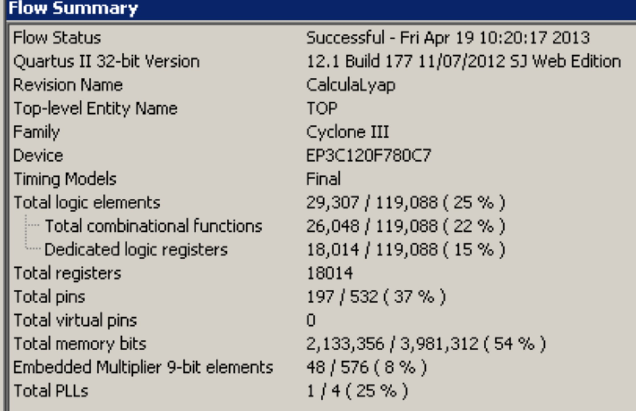
\includegraphics[width=1\columnwidth]{compilacion.pdf}\\
	\caption{Compilation report of the \textit{MLE} calculator.}\label{fig:compilacion}
\end{figure}

En la figura \ref{fig:st} se muestra la salida del Signal Tap.
La señal \textit{salida} es la suma de los $MLE$ luego de cada iteración.
La segunda señal llamada \textit{cuenta\_sal} corresponde a la sumatoria actual.
Finalmente, cada flanco descendente de la señal \textit{listoD1} indica que la salida es un dato válido.
La salida fué procesada con Matlab para obtener la curva mostrada en la figura\ref{fig:lyapu}.
El valor del MLE en la iteración $250000$ es $0.1415$, lo que es consistente con el MLE obtenido con Matlab.
%
\begin{figure*}
	\centering
	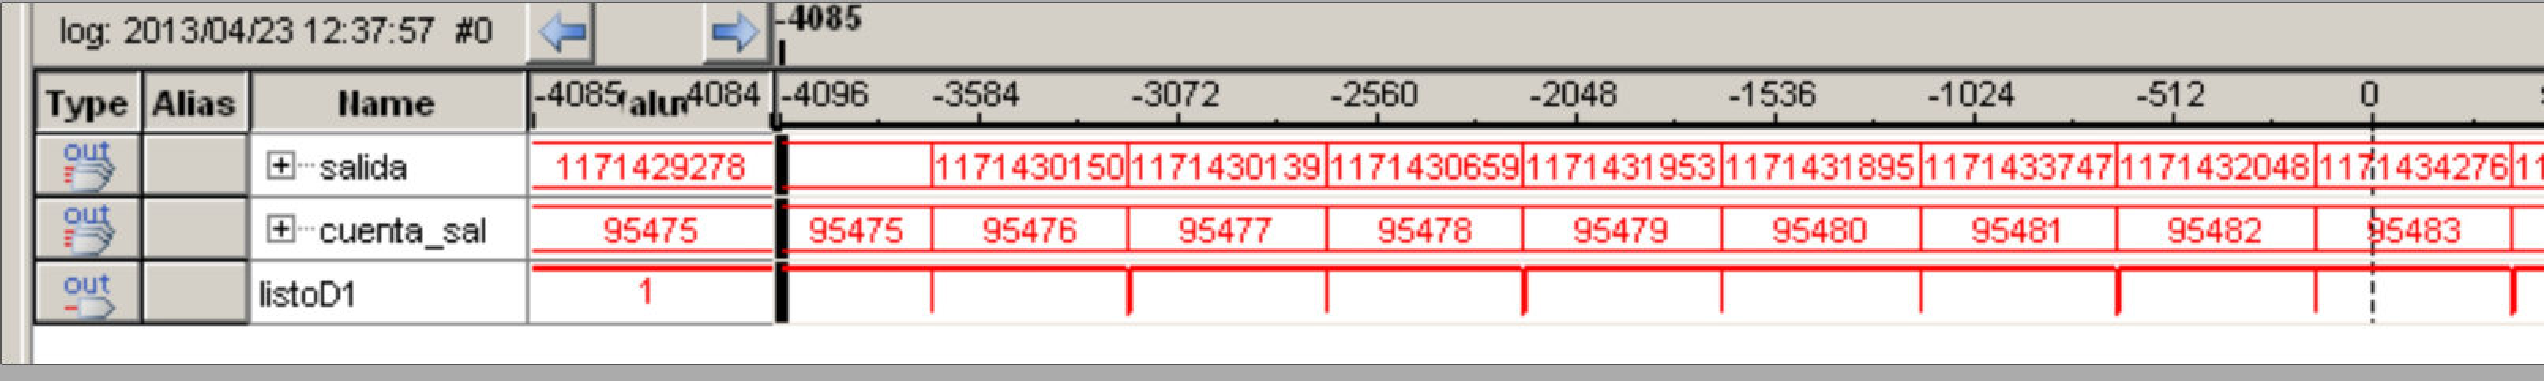
\includegraphics[width=1\columnwidth]{st.pdf}\\
	\caption{Salida del Signal Tap.}\label{fig:st}
\end{figure*}
%
\begin{figure}
	\centering
	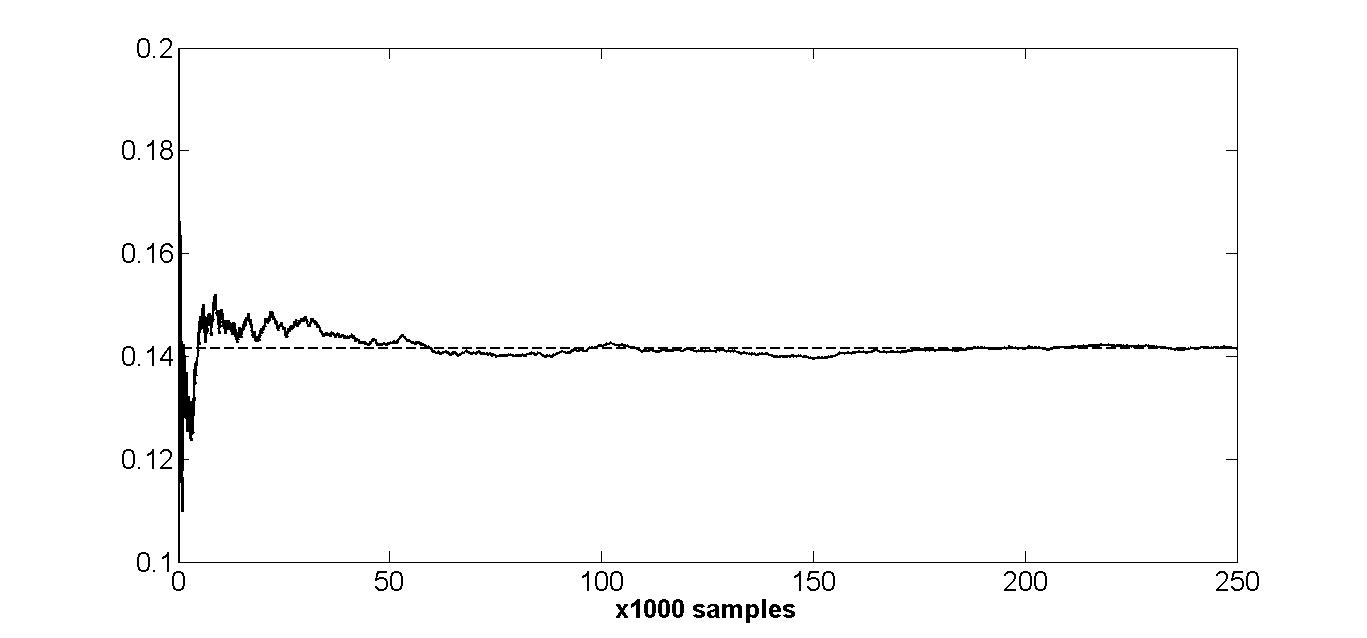
\includegraphics[width=1\columnwidth]{Lyap_MATLAB.jpg}\\
	\caption{Convergencia del algoritmo que calcula el MLE.}\label{fig:lyapu}
\end{figure}


\subsubsection{Estado actual del avance}

Actualmente estamos en etapa de desarrollo de la implementación en hardware de este algoritmo.
En este segundo caso, el sistema bajo prueba es la familia de mapas cuadráticos bidimensionales descriptos en el capítulo \ref{sec:QMaps}.

La población inicial es de $12$ coeficientes iniciales del mapa caótico empleado.
En la figura \ref{bloques} puede verse un diagrama en bloques general del sistema.
Este consiste en dos bloques principales conectados al sistema caótico bajo prueba a través de una interface wishbone.
Esto independiza el sistema del cuantificador y permite cambiar fácilmente el sistema bajo prueba.
%
\begin{figure}
	\centering
	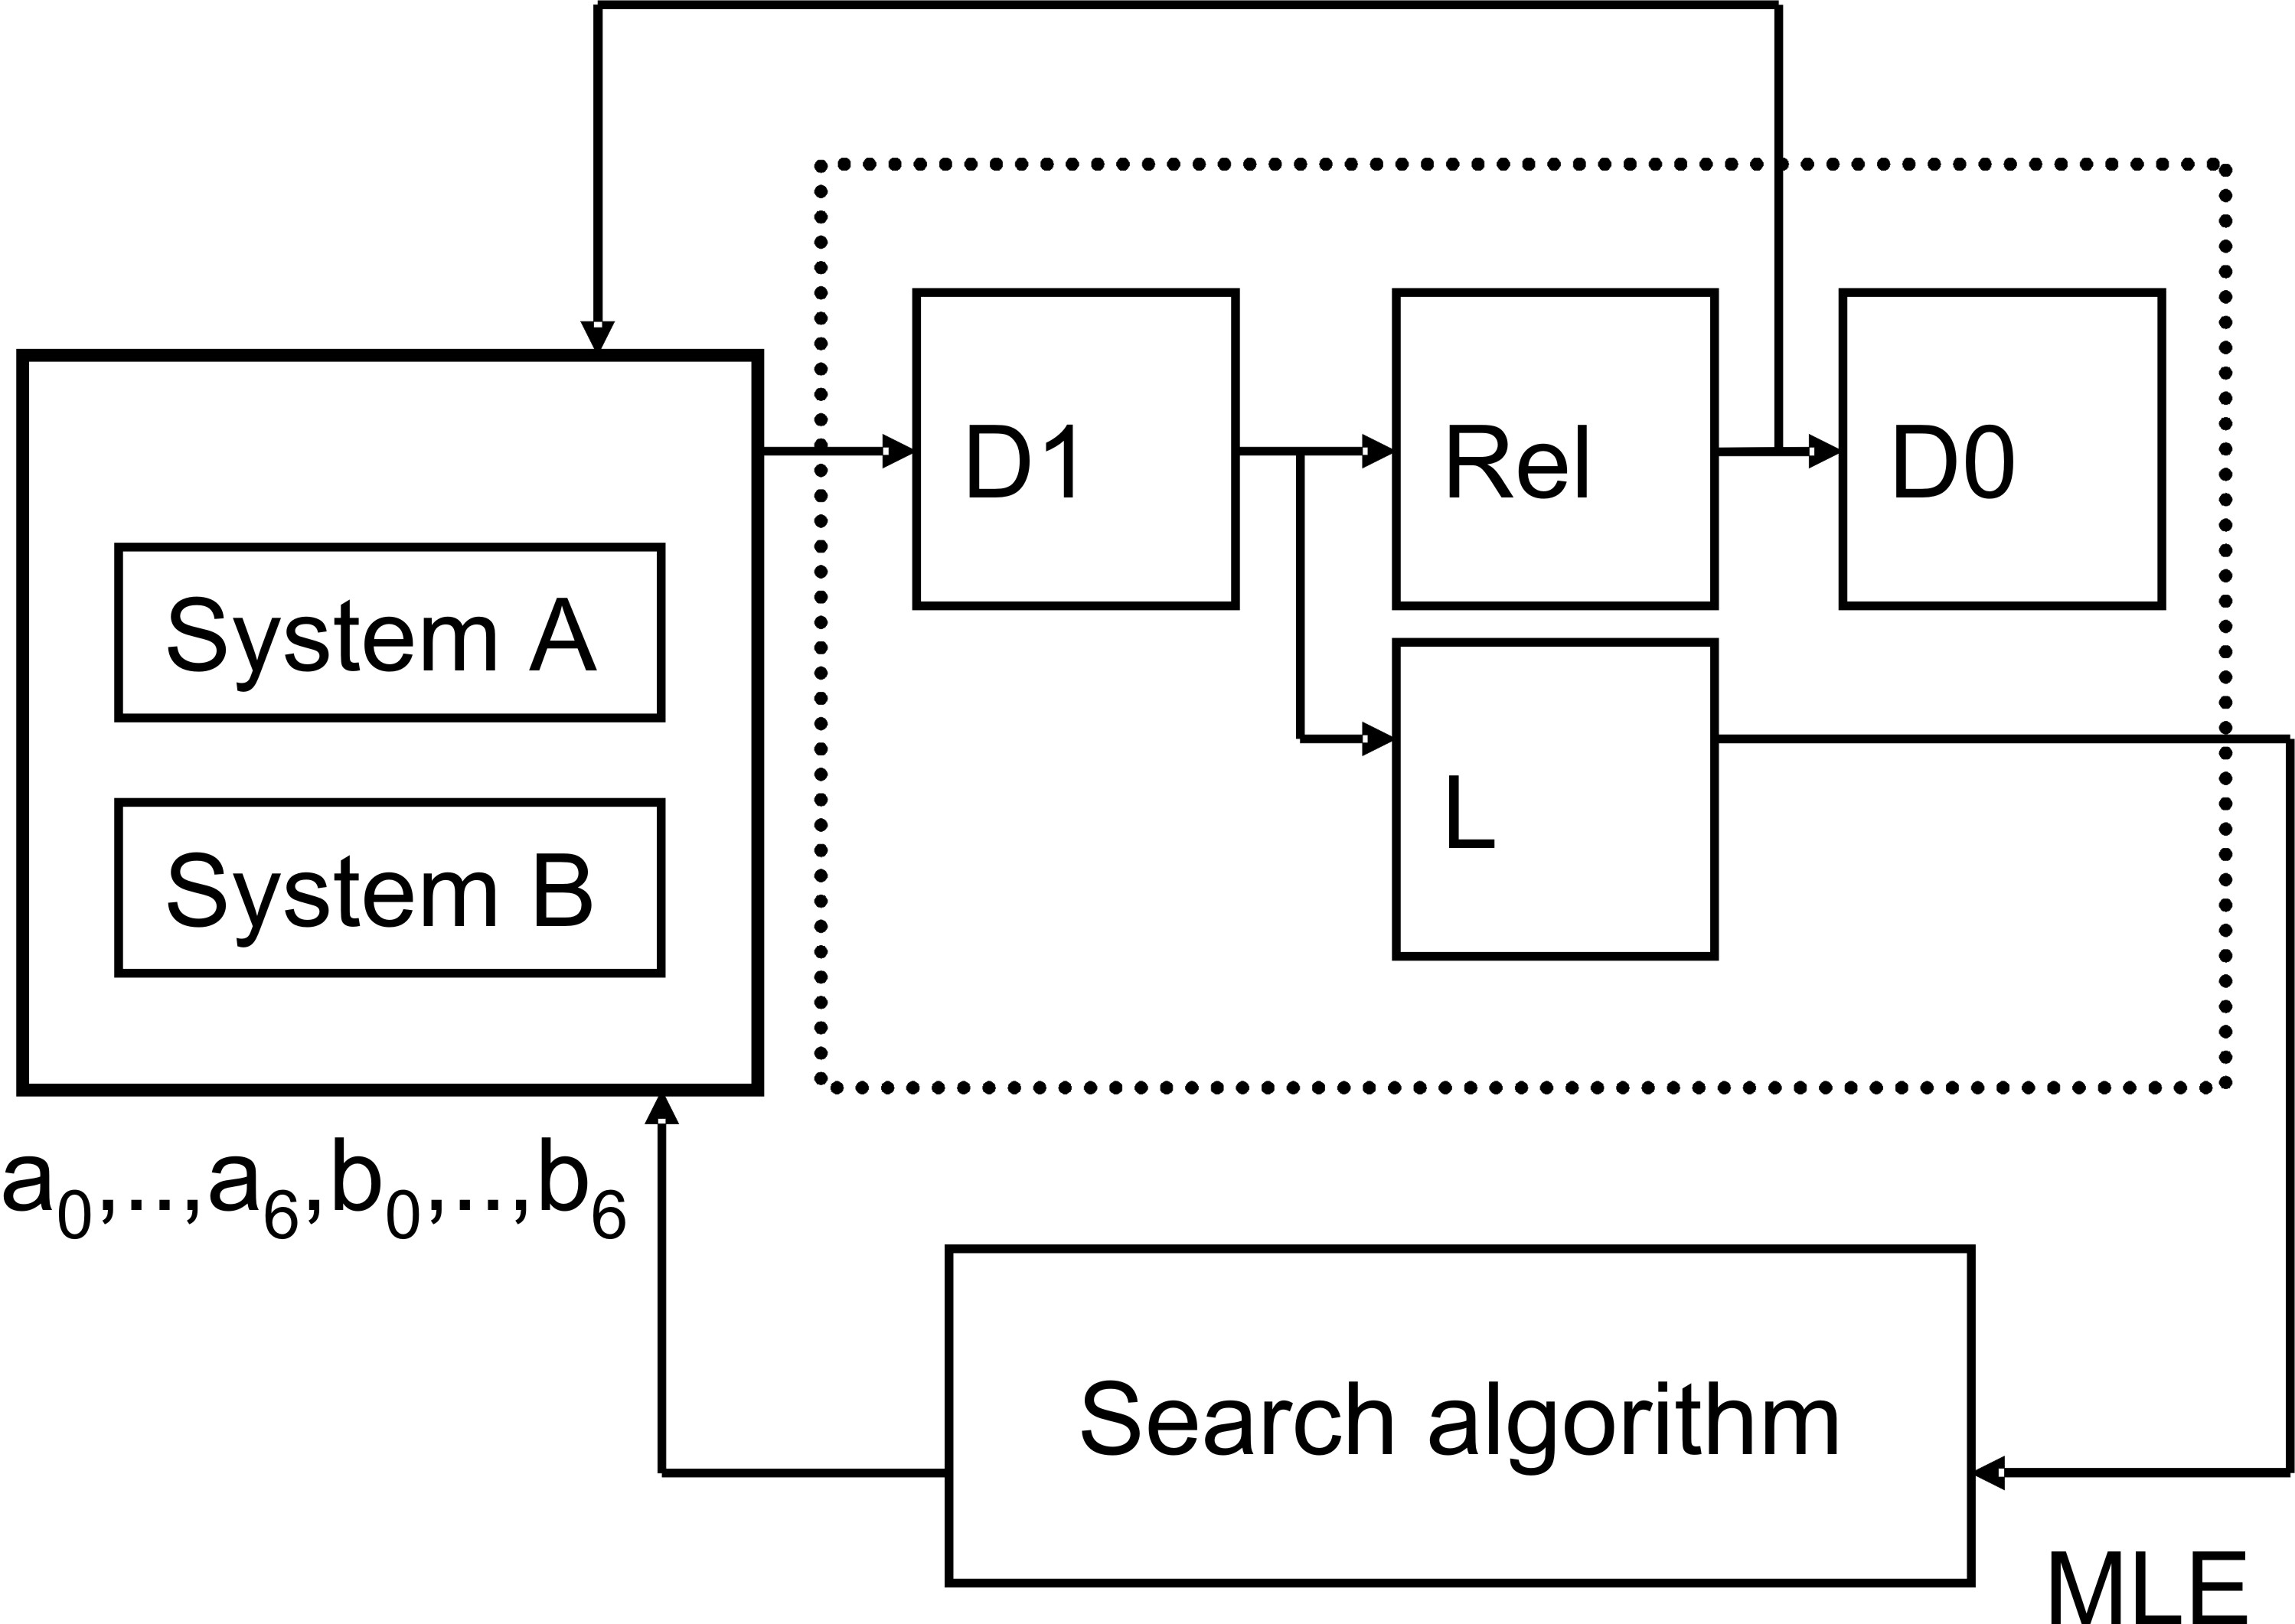
\includegraphics[width=0.85\columnwidth]{bloques.jpg}\\
	\caption{Diagrama en bloques del sistema implementado en FPGA.}\label{bloques}
\end{figure}

El sistema caótico es duplicado en dos bloques, $System A$ y $System B$.
Cada uno de ellos es inicializado con los puntos en el espacio de fases	($x_{a(i-1)}$,$y_{a(i-1)}$) y ($x_{br(i-1)}$,$y_{br(i-1)}$) respectivamente.
Cuando los sistemas caóticos terminan de calcular sus salidas, la señal digital \textit{habilita} se pone en cero y el bloque $D1$ es habilitado para calcular la distancia euclideana entre las salidas ($x_{a(i)}$,$y_{a(i)}$) y ($x_{br(i)}$,$y_{br(i)}$).

Luego se habilitan los bloques concurrentes $L$ y $Rel$.
Los puntos relocalizados que alimentan al bloque $System B$ son calculados por el bloque $Rel$.
Este bloque solo necesita los valores actuales de $d_1$ los valores previos de $d_0$, como se muestra en la ecuación \ref{eq:reubicacion}.
Cuando los puntos relocalizados $x_{br(i)}$ y $y_{br(i)}$ están disponibles, los bloques $System A$ y $System B$ se habilitan para obtener la siguiente iteración.
También se habilita el bloque $D_0$ para calcular el valor actual de $d_{0(i)}$, que se utilizará en la siguiente iteración.

Finalmente, el bloque $L$ realiza la división entre $d_0$ y $d_1$ para luego calcular el valor absoluto y el logaritmo de esta división.
El mapa es iterado $N=250000$ veces y el resultado de la sumatoria dividido por $N$ para asegurar la convergencia del método.

Cada bloque fue implementado utilizando lenguaje VHD e IP \textit{cores} provistos por \textit{Altera} (\textit{megafunctions}) cada vez que fue posible, debido a que estos \textit{cores} están optimizados para este dispositivo.
Las operaciones de punto flotante como las sumas, multiplicaciones, valores absolutos y logaritmos fueron calculadas con dichas \textit{megafunctions}.

La figura \ref{D1} muestra la implementación del bloque $D1$ en el entorno gráfico Quartus
Los puntos de salida y entrada $a$ y $b$, son tomados luego de que la señal \textit{habilita} se pone en cero.
Entonces, las señales son procesadas de acuerdo a la ecuación \ref{eq:D0D1} para calcular la distancia euclideana $d_1$.
%
\begin{figure*}
	\centering
	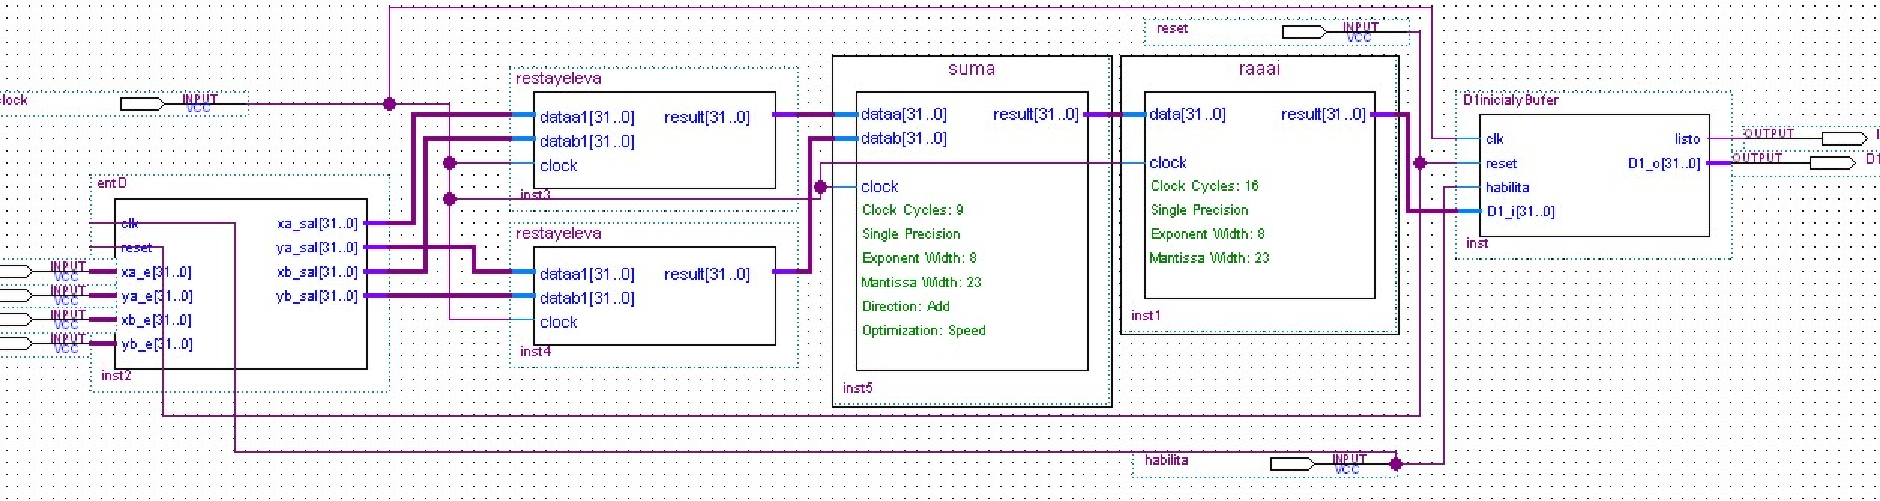
\includegraphics[width=1\columnwidth]{D1.pdf}\\
	\caption{Bloque $D_1$.}\label{D1}
\end{figure*}

La lógica del algoritmo genético fue implementada en lenguaje VHD.
Esta lógica junto con el registro de los $12$ coeficientes se muestran en la figura \ref{fig:evolutivecircuit}.
También se muesran los resultados de la compilación en la figura \ref{fig:alg_comp}.
Puede verse que esta implementación ocupa pocos recursos del dispositivo.
%
\begin{figure*}
	\centering
	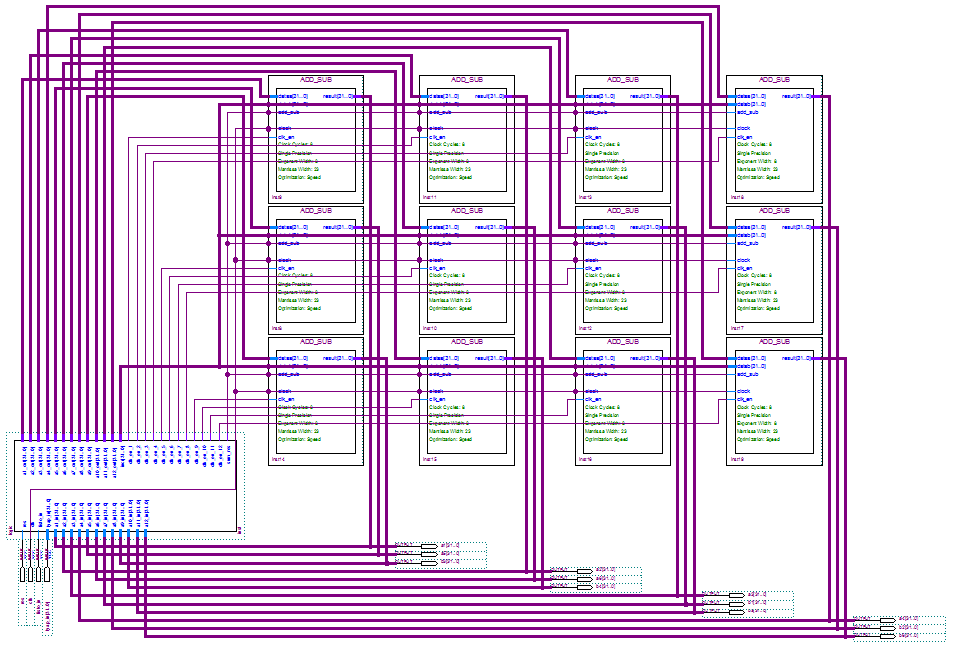
\includegraphics[width=1\columnwidth]{evolutive.png}\\
	\caption{Circuito del algoritmo evolutivo. Cada uno de los $12$ bloques ADD\_SUB guarda el valor de uno de los coeficientes $a_i$.}\label{fig:evolutivecircuit}
\end{figure*}
%
\begin{figure}
	\centering
	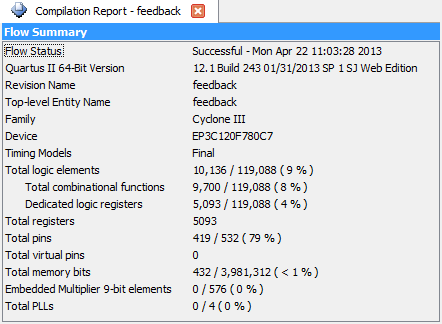
\includegraphics[width=1\columnwidth]{compilationreportalgoritmo.png}\\
	\caption{Compilation report del algoritmo evolutivo.}\label{fig:alg_comp}
\end{figure}
\section{Cuantificadores de la teoría de la información}
\label{sec:ITQs}

Dada una fuente de símbolos cuya salida es un vector de símbolos $X$, existen diferentes procedimientos para obtener una PDF \cite{Rosso2009, DeMicco2008, Mischaikow1999, Powell1979, Rosso2001, Pompe2002}.
La determinación de la mejor PDF $P$ es un problema fundamental porque $P$ y el espacio de muestra $X$ están inextricablemente vinculados.
Su aplicabilidad depende de las características particulares de los datos, tales como estacionariedad, duración de la serie temporal, variación de los parámetros, nivel de contaminación de ruido, etc.

Los cuantificadores seleccionados se basan en el recuento de símbolos y en la estadística de patrones de orden.
Las métricas a utilizar pueden clasificarse de forma amplia en dos categorías: las que cuantifican el \textit{contenido de información} de los datos en comparación con los relacionados con su \textit{complejidad}.
Obsérvese que aquí nos estamos refiriendo al espacio de funciones de densidad de probabilidad, no al espacio físico.
Para clarificar y simplificar, introducimos solamente los cuantificadores de la Teoría de la Información que se definen en PDFs discretas, ya que solo estamos tratando con datos discretos (series temporales).
Sin embargo, todos los cuantificadores también tienen definiciones para el caso continuo \cite{Shannon1948}.

\subsection{Entropía de Shannon y Complejidad Estadística}

La entropía es una cantidad básica que puede considerarse como una medida de la incertidumbre asociada (información) al proceso físico descrito por $P$.
Al tratar con el contenido de la información, la entropía de Shannon se considera a menudo como la fundamental y más natural \cite{Shannon1948}.
Considerada como una medida de la incertidumbre, es el ejemplo más paradigmático de estos cuantificadores de información.

Sea $P=\{p_i; i=1,\ldots, N\}$ con $\sum_{i=1}^N p_i = 1$, una distribución de probabilidad discreta, con $N$ el número de estados posibles del sistema bajo estudi.
La medida de la información logarítmica de shannon se denota como
\begin{equation}
\label{Shannon-disc}
S[P] ~=~ -\sum_{i=1}^{N} p_i \ln \left[ p_i \right] \ .
\end{equation}

Si $S[P] = S_{\min} = 0$, estaremos en posición de predecir con total certeza cuáles de los posibles resultados $i$, cuyas probabilidades están dadas por $p_i$, tendrán lugar realmente.
Nuestro conocimiento del proceso subyacente descrito por la distribución de probabilidad es máximo en este caso.
Por el contrario, nuestro conocimiento es mínimo para una distribución uniforme $P_e = \{p_i = 1/N; i = 1, \ldots, N \}$ dado que cada resultado exhibe la misma probabilidad de ocurrencia, y la incertidumbre es máxima, es decir, $S[P_e] = S_{\ max} = \ln N$.
Estas dos situaciones son casos extremos, por lo tanto nos centramos en la entropía de Shannon "normalizada", $0 \leq H \leq 1$, dada como
\begin{equation}
\label{shannon-disc-normalizada}
H[P] = S[P] / S_{\max} \ .
\end{equation}

Contrariamente al contenido de la información, no existe una definición universalmente aceptada de complejidad.
Aquí, nos centramos en describir la \textit{complejidad de las series temporales} y no nos referimos a la complejidad de los \textit{sistemas} subyacentes.
Un sistema complejo no genera necesariamente una salida compleja.
De hecho, los modelos "simples" pueden generar datos complejos, mientras que los sistemas "complicados" pueden producir datos de salida de baja complejidad \cite{Kantz1998}.

Una noción intuitiva de una complejidad cuantitativa atribuye valores bajos tanto a datos perfectamente ordenados (es decir, con entropía de Shannon que se va desapareciendo) como a datos aleatorios no correlacionados (con entropía Shannon máxima).
Por ejemplo, la complejidad estadística de una simple oscilación o tendencia (ordenada), pero también de ruido blanco no correlacionado (no ordenado) sería clasificada como baja.
Entre los dos casos de mínima y máxima entropía, los datos son más difíciles de caracterizar y por lo tanto la complejidad debe ser mayor.
Buscamos alguna función $C[P]$ que cuantifique las estructuras presentes en los datos que se alejan de estos dos casos.
Estas estructuras se relacionan con la organización, la estructura correlacional, la memoria, la regularidad, la simetría, los patrones y otras propiedades \cite{Feldman2008}.

Asumimos que el grado de estructuras correlacionales sería capturado adecuadamente por algún funcional $C[P]$ de la misma manera que la entropía de Shannon $S[P]$ \cite{Shannon1948} ``capta " la aleatoriedad.
Claramente, las estructuras ordinales presentes en un proceso no son cuantificadas por medidas de aleatoriedad y, por consiguiente, son necesarias medidas de complejidad estadística o estructural para una mejor comprensión (caracterización) de la dinámica del sistema representada por sus series temporales \cite{Feldman1998}.

Una medida adecuada de complejidad puede definirse como el producto de una medida de información y una medida de desequilibrio, es decir, algún tipo de distancia de la distribución equiprobable de los estados accesibles de un sistema.
En este sentido, en \cite{Lamberti2004} los autores introdujeron una eficaz {\it Medida de Complejidad Estadística \/} (SCM) $C$, que es capaz de detectar detalles esenciales de los procesos dinámicos subyacentes al conjunto de datos.
Basado en el trabajo de López-Ruiz \cite{Lopez1995}, esta medida de complejidad estadística \cite{Martin2003,Lamberti2004} se define a través de la forma del producto
\begin{equation}
C[P] = Q_{J}[P,P_e] \cdot H[P]
\label{complexity}
\end{equation}
de la entropía de Shannon normalizada $H$, ver eq. \eqref{shannon-disc-normalizada}, y el desequilibrio $Q_{J}$ definido en términosde la divergencia de Jensen-Shannon $J[P, P_e]$.
Esto es,
\begin{equation}
\label{disequilibrium}	
Q_{J} [ P, P_e] = Q_{0} J[ P, P_e] = Q_{0} \{ S[(P + P_e)/2 ] - S[ P ]/2 - S[P_e]/2\},
\end{equation}
en la divergencia de Jensen-Shannon mencionada arriba, $Q_0$ es una constante de normalización tal que $0 \leq Q_{J} \leq 1$:
\begin{equation}
Q_0 ~=~ -2 \left\{ {\frac{N+1}{N}} \ln (N+1) - \ln (2N) + \ln N \right\}^{-1} \ ,
\label{q0-jensen-1}
\end{equation}
y es igual a la inversa del máximo valor posible de $J [P,P_e]$.
Este valor es obtenido cuando una de las componentes de $P$, digamos $p_m$, es igual a uno y todos los $p_j$ restantes son cero.

La divergencia de Jensen-Shannon, que cuantifica la diferencia entre las distribuciones de probabilidad, es especialmente útil para comparar la composición simbólica entre diferentes secuencias \cite{Grosse2002}.
Obsérvese que la SCM introducida anteriormente depende de dos distribuciones de probabilidad diferentes: una asociada con el sistema analizado, $P$, y la otra con la distribución uniforme, $P_e$.
Además, se demostró que para un valor dado de $H$, el rango de valores posibles de $C$ varía entre un mínimo $C_ {min}$ y un máximo $C_ {max}$, restringiendo los posibles valores del SCM \cite{Martin2006}.

Por lo tanto, está claro que información adicional importante relacionada con la estructura correlacional entre los componentes del sistema físico se proporciona evaluando la medida de la complejidad estadística.

\subsection{Determinación de la distribución de probabilidad}

La evaluación de los cuantificadores derivados de la Teoría de la Información supone algún conocimiento previo sobre el sistema; específicamente para aquellos introducidos previamente (entropía de Shannon y complejidad estadística), una distribución de probabilidad asociada a la serie temporal en análisis debe proporcionarse antes.
La determinación del PDF más adecuado es un problema fundamental porque la PDF $P$ y el espacio de muestra $\Omega$ están intrincadamente vinculados.

Las metodologías usuales asignan a cada valor de la serie $X(t)$ (o conjunto de valores consecutivos no superpuestos) un símbolo de un alfabeto finito $A = \{a_1, \dots, a_M \}$, creando así una {\it secuencia simbólica \/} que puede considerarse como una descripción de la serie cronológica en cuestión.
Como consecuencia, las relaciones de orden y las escalas temporales de la dinámica se pierden por completo.

Es importante resltar que $P$ en si, no es un objeto con una definición única y existen varias aproximaciones para ``asociar'' una dada $P$ con una dada serie de tiempo.
Solo para mencionar algunos criterios de extracción utilizados frecuentemente en la literatura: {\it a)\/} histogramas de series temporales \cite{Martin2004}, {\it b)\/} dinámica simbólica binaria \cite{Mischaikow1999}, {\it c)\/} análisis de Fourier \cite{Powell1979}, {\it d)\/} trensformadas wavelet \cite{Blanco1998,Rosso2001}, {\it e)\/} PDF de particiones \cite{Ebeling2001}, {\it f)\/} PDF de permutaciones \cite{Pompe2002,Keller2005}, {\it g)\/} PDF discreta \cite{Amigo2007}, etc.
Hay una amplia libertad para elegir entre ellas y la aplicación específica debe ser analizada para hacer una buena elección.

Se puede incorporar debidamente la información causal si se incluye información sobre la dinámica pasada del sistema en la secuencia simbólica, es decir, los símbolos del alfabeto $A$ se asignan a una porción del espacio de fase o trayectoria.
Bandt y Pompe (BP) \cite{Bandt2002} introdujeron una metodología simbólica simple y robusta que toma en cuenta el ordenamiento temporal de las series temporales comparando valores vecinos en una serie temporal.
La propiedad de causalidad de la PDF permite que los cuantificadores (basados en esta PDF) discriminan entre sistemas determinísticos y estocásticos \cite{Rosso2007B}.
Los datos simbólicos son:
{\it (i) \/} ~ creados por la clasificación de los valores de la serie; y
{\it (ii) \/} ~ definidos por el reordenaminto de los datos embebidos en orden ascendente, lo que equivale a una reconstrucción de espacio de fase con dimensión de emmbedding (longitud de patrón) $D$ y retardo de tiempo $\tau$.
De esta forma, es posible cuantificar la diversidad de los símbolos de ordenación (patrones) derivados de una serie temporal escalar.
Obsérvese que la secuencia de símbolos apropiada surge naturalmente de la serie temporal, y no se necesitan suposiciones basadas en modelos.
El procedimiento es el siguiente:
\begin{itemize}
	\item Dada una serie $\{x_t; t=0, \Delta t, \cdots,N\Delta t \}$, se genera una secuencia de vectores de longitud $D$.
	\begin{equation}
	(s)\longmapsto\left(x_{t-(d-1)\Delta t},x_{t-(d-2)\Delta t},\dots,x_{t-\Delta t},x_{t}\right) 
	\label{eq:vectores}
	\end{equation}
	Cada vector resulta ser la "historia" del valor $x_t$. Evidentemente, cuanto más larga sea la longitud de los vectores $D$, mayor será la información sobre la historia de los vectores, pero se requiere un valor más alto de $N$ para tener una estadística adecuada.
	\item Las permutaciones $\pi=(r_0, r_1, \cdots, r_{D-1})$ de $(0, 1, \cdots, D-1)$ es llamado ``patrón de orden'' de tiempo $t$, definido por:
	\begin{equation}
	\label{eq:permuta}
	x_{t-r_{D-1}\Delta t}\le x_{t-r_{D-2}\Delta t}\le\dots\le x_{t-r_{1}\Delta t}\le x_{t-r_0\Delta t}
	\end{equation}
	Para obtener se un resultado único se considera $r_i<r_{i-1}$ si $x_{t-r_{i}\Delta t}=x_{t-r_{i-1}\Delta t}$.
	De esta forma, todas las $D!$ permutaciones posibles $\pi$ de orden $D$, y la PDF $P=\{p(\pi)\}$ es definida como:
	\begin{equation}
	\label{eq:frequ}
	p(\pi)=\frac{\sharp \{s|s\leq N-D+1; (s) \quad \texttt{has type}~\pi\}}{N-D+1}
	\end{equation}
	En estas últimas expresiones, el símbolo $\sharp$ denota cardinalidad.
\end{itemize}

Por lo tanto, una distribución de probabilidad de patrones de órden $P = \{ p(\pi_i), i = 1, \dots, D! \}$ se obtiene de la serie temporal.
De esta manera, el vector definido por la ecuación \eqref{eq:frequ} se convierte en un símbolo único $\pi$.
Se establece $r_i < r_{i-1}$ si $x_{s-r_{i}} = x_{s-r_{i-1}}$ para la obtener una única solución.
La única condición para la aplicabilidad del método BP es una suposición estacionaria muy débil: para $k \leq D$, la probabilidad para $x_t<x_{t + k}$ no debe depender de $t$.
Con respecto a la selección de los parámetros, Bandt y Pompe sugirieron trabajar con $3 \leq D \leq 6$ para longitudes de series de tiempo típicas, y específicamente se consideró un retraso de tiempo $\tau = 1$ en su publicación principal.

Para destacar la diferencia entre una $P$ \textit{causal} y una \textit{no causal}, consideremos una serie de valores $X=\{x_i,~i=1,2,...\}$ generada por la función $randn$ de Matlab's $^\copyright$; consideremos también la serie $Y=\{y_i,~i=1,2,...\}$ como la resultante de ordenar la serie $X$ en forma ascendente. Esto se puede ver en el ejemplo en la figura \ref{fig:causal_nocausal}, en la figura \ref{subfig:causal_nocausal_x} se muestran 1000 valores sorteados con una distribución uniforme entre 0 y 1, también mostramos en la figura \ref{subfig:causal_nocausal_y} la versión ordenada de la serie de la figura \ref{subfig:causal_nocausal_x}, son los mismos valores pero ordenados en forma ascendente. Una $P$ no causal es el histograma normalizado que mostramos en las figuras \ref{subfig:causal_nocausal_HistValx} y \ref{subfig:causal_nocausal_HistValy}, en donde puede verse que $P(X)$ es idéntica a $P(Y)$, por lo que todos los cuantificadores que se calculen a partir de ellas serán idénticos para las dos series. Una $P$ causal puede ser obtenida mediante el procedimiento de Bandt \& Pompe descripto arriba, en este caso $P(X)$ de la figura \ref{subfig:causal_nocausal_HistBPx} es bastante uniforme y $P(Y)$ de la figura \ref{subfig:causal_nocausal_HistBPy} tiene una forma tipo delta. En este caso, $P$ registra que $Y$ es monótonamente creciente y presenta un solo patrón de orden.

\begin{figure}[htpb]
	\centering
	\begin{subfigure}[t]{0.49\textwidth}
		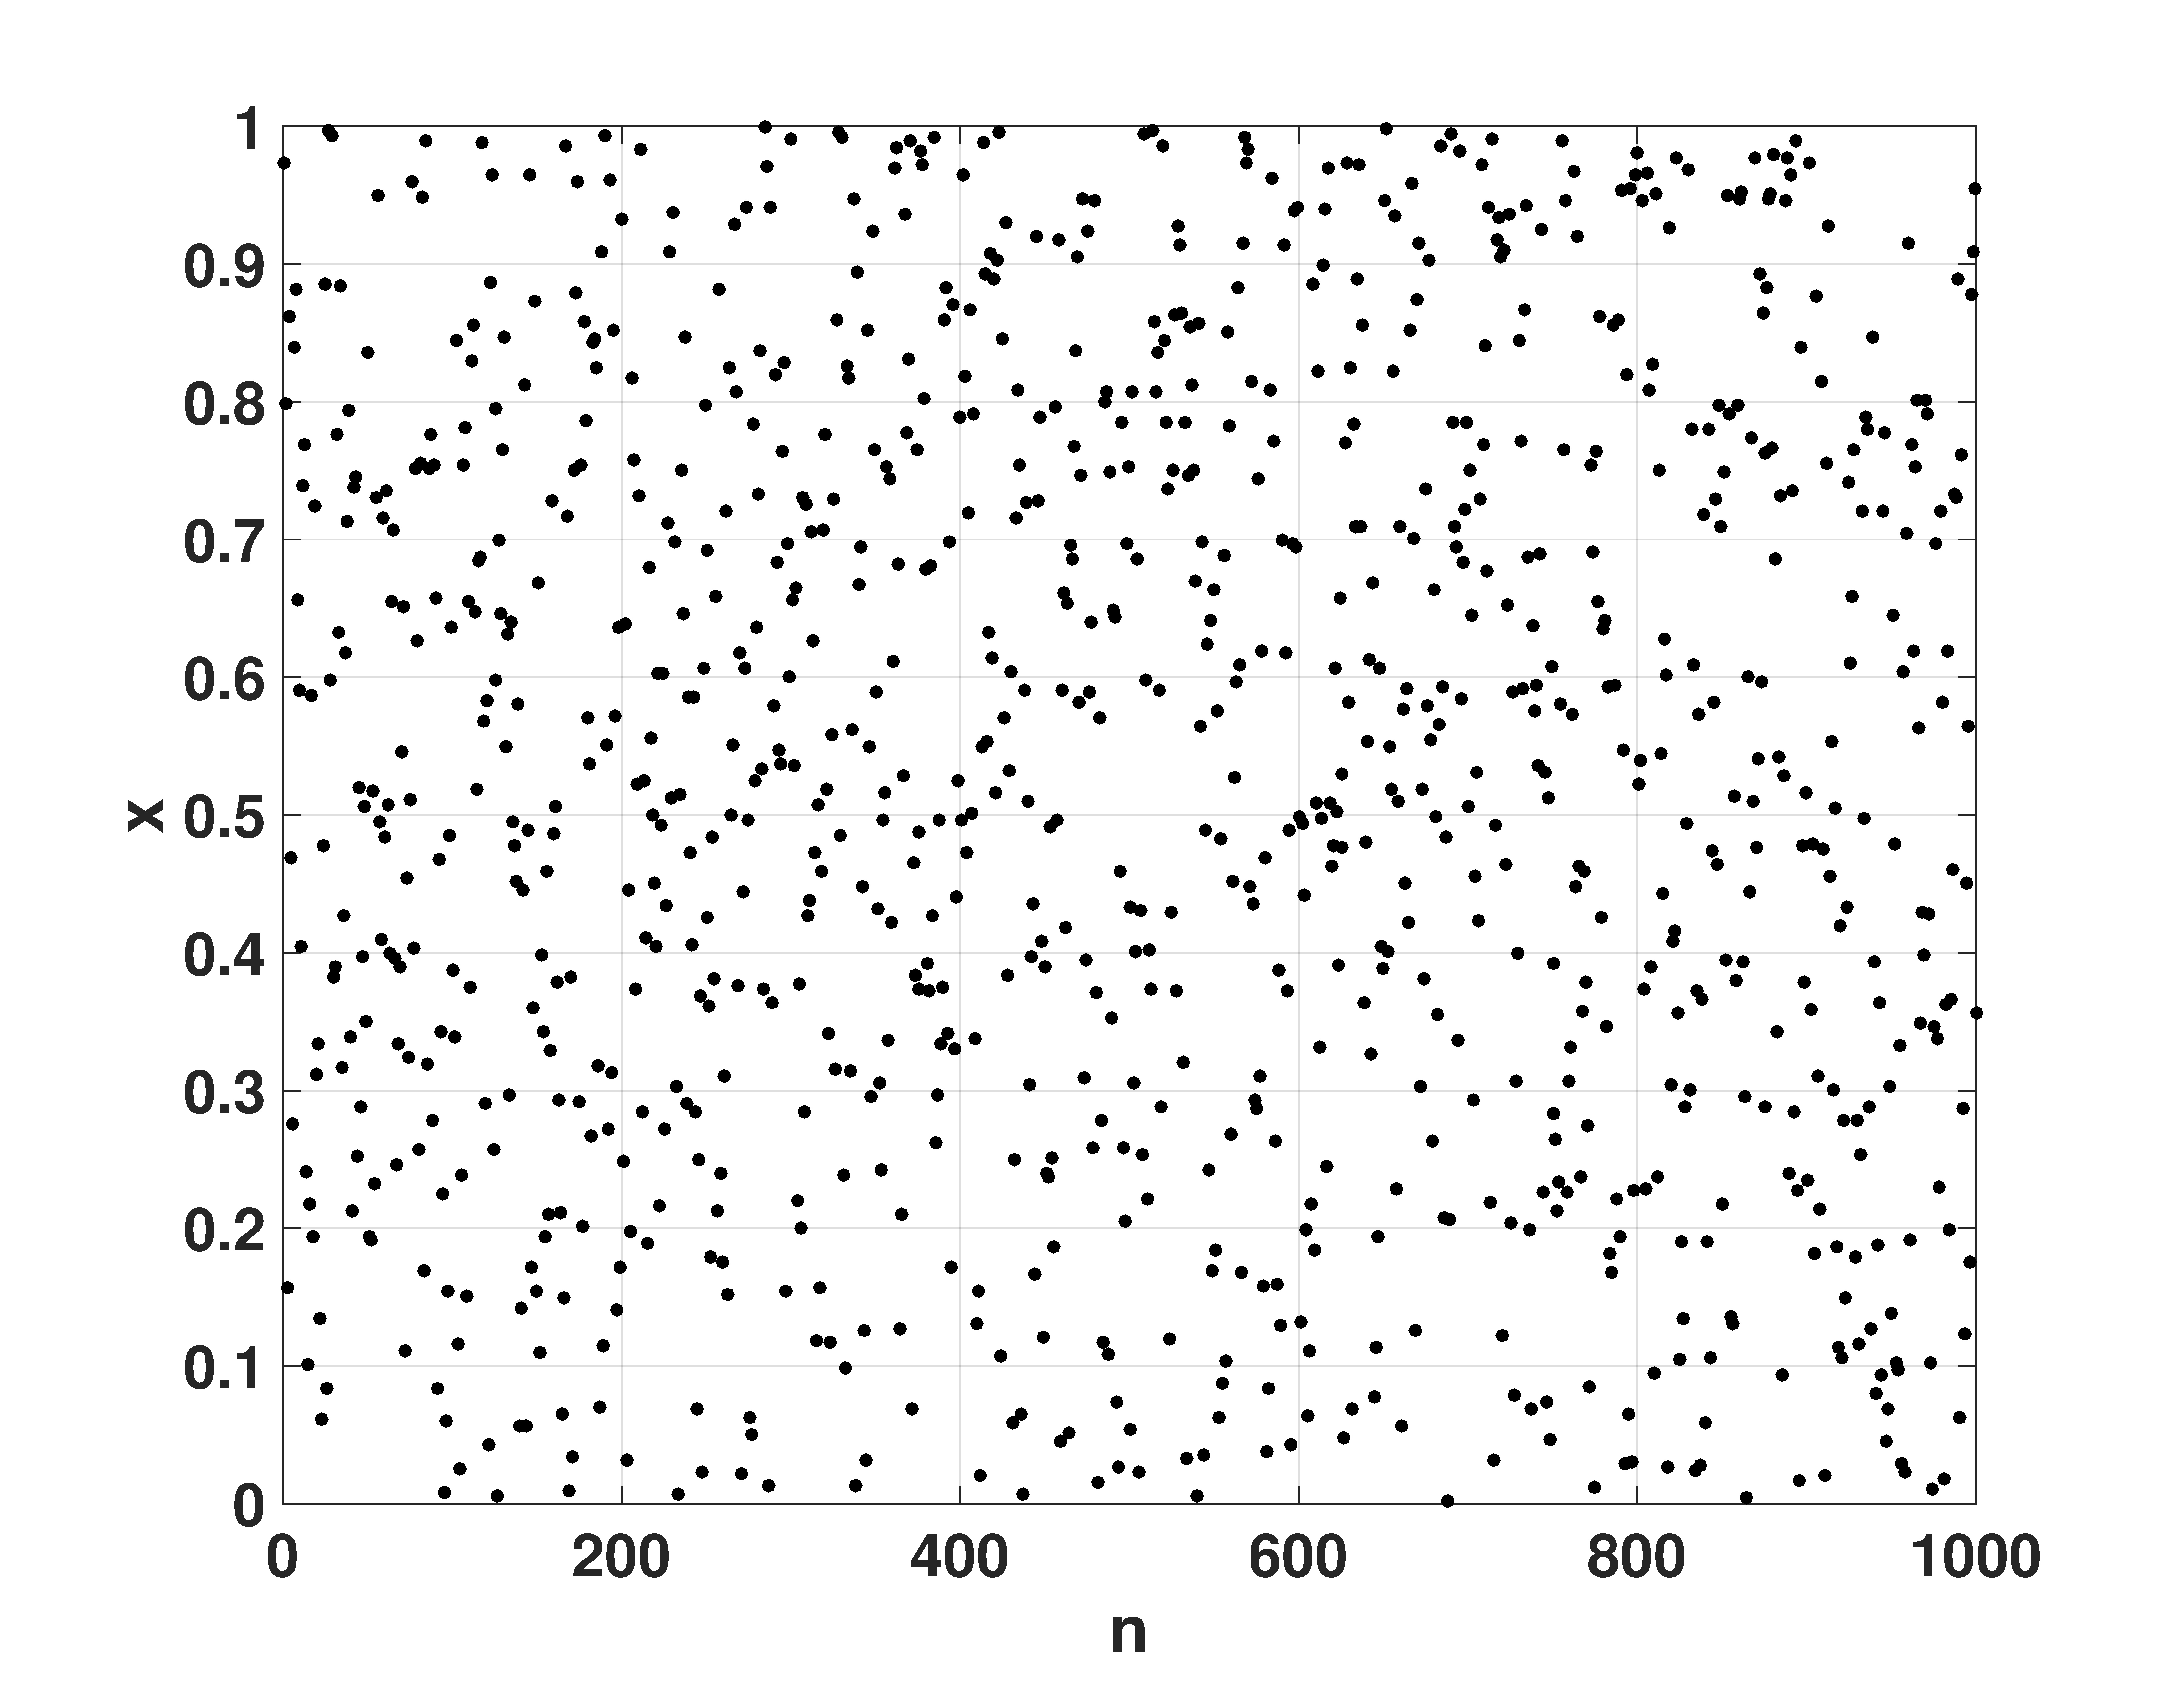
\includegraphics[width=\textwidth]{x}
		\caption{$1000$ puntos con distribución uniforme}
		\label{subfig:causal_nocausal_x}
	\end{subfigure}
	\begin{subfigure}[t]{0.49\textwidth}
		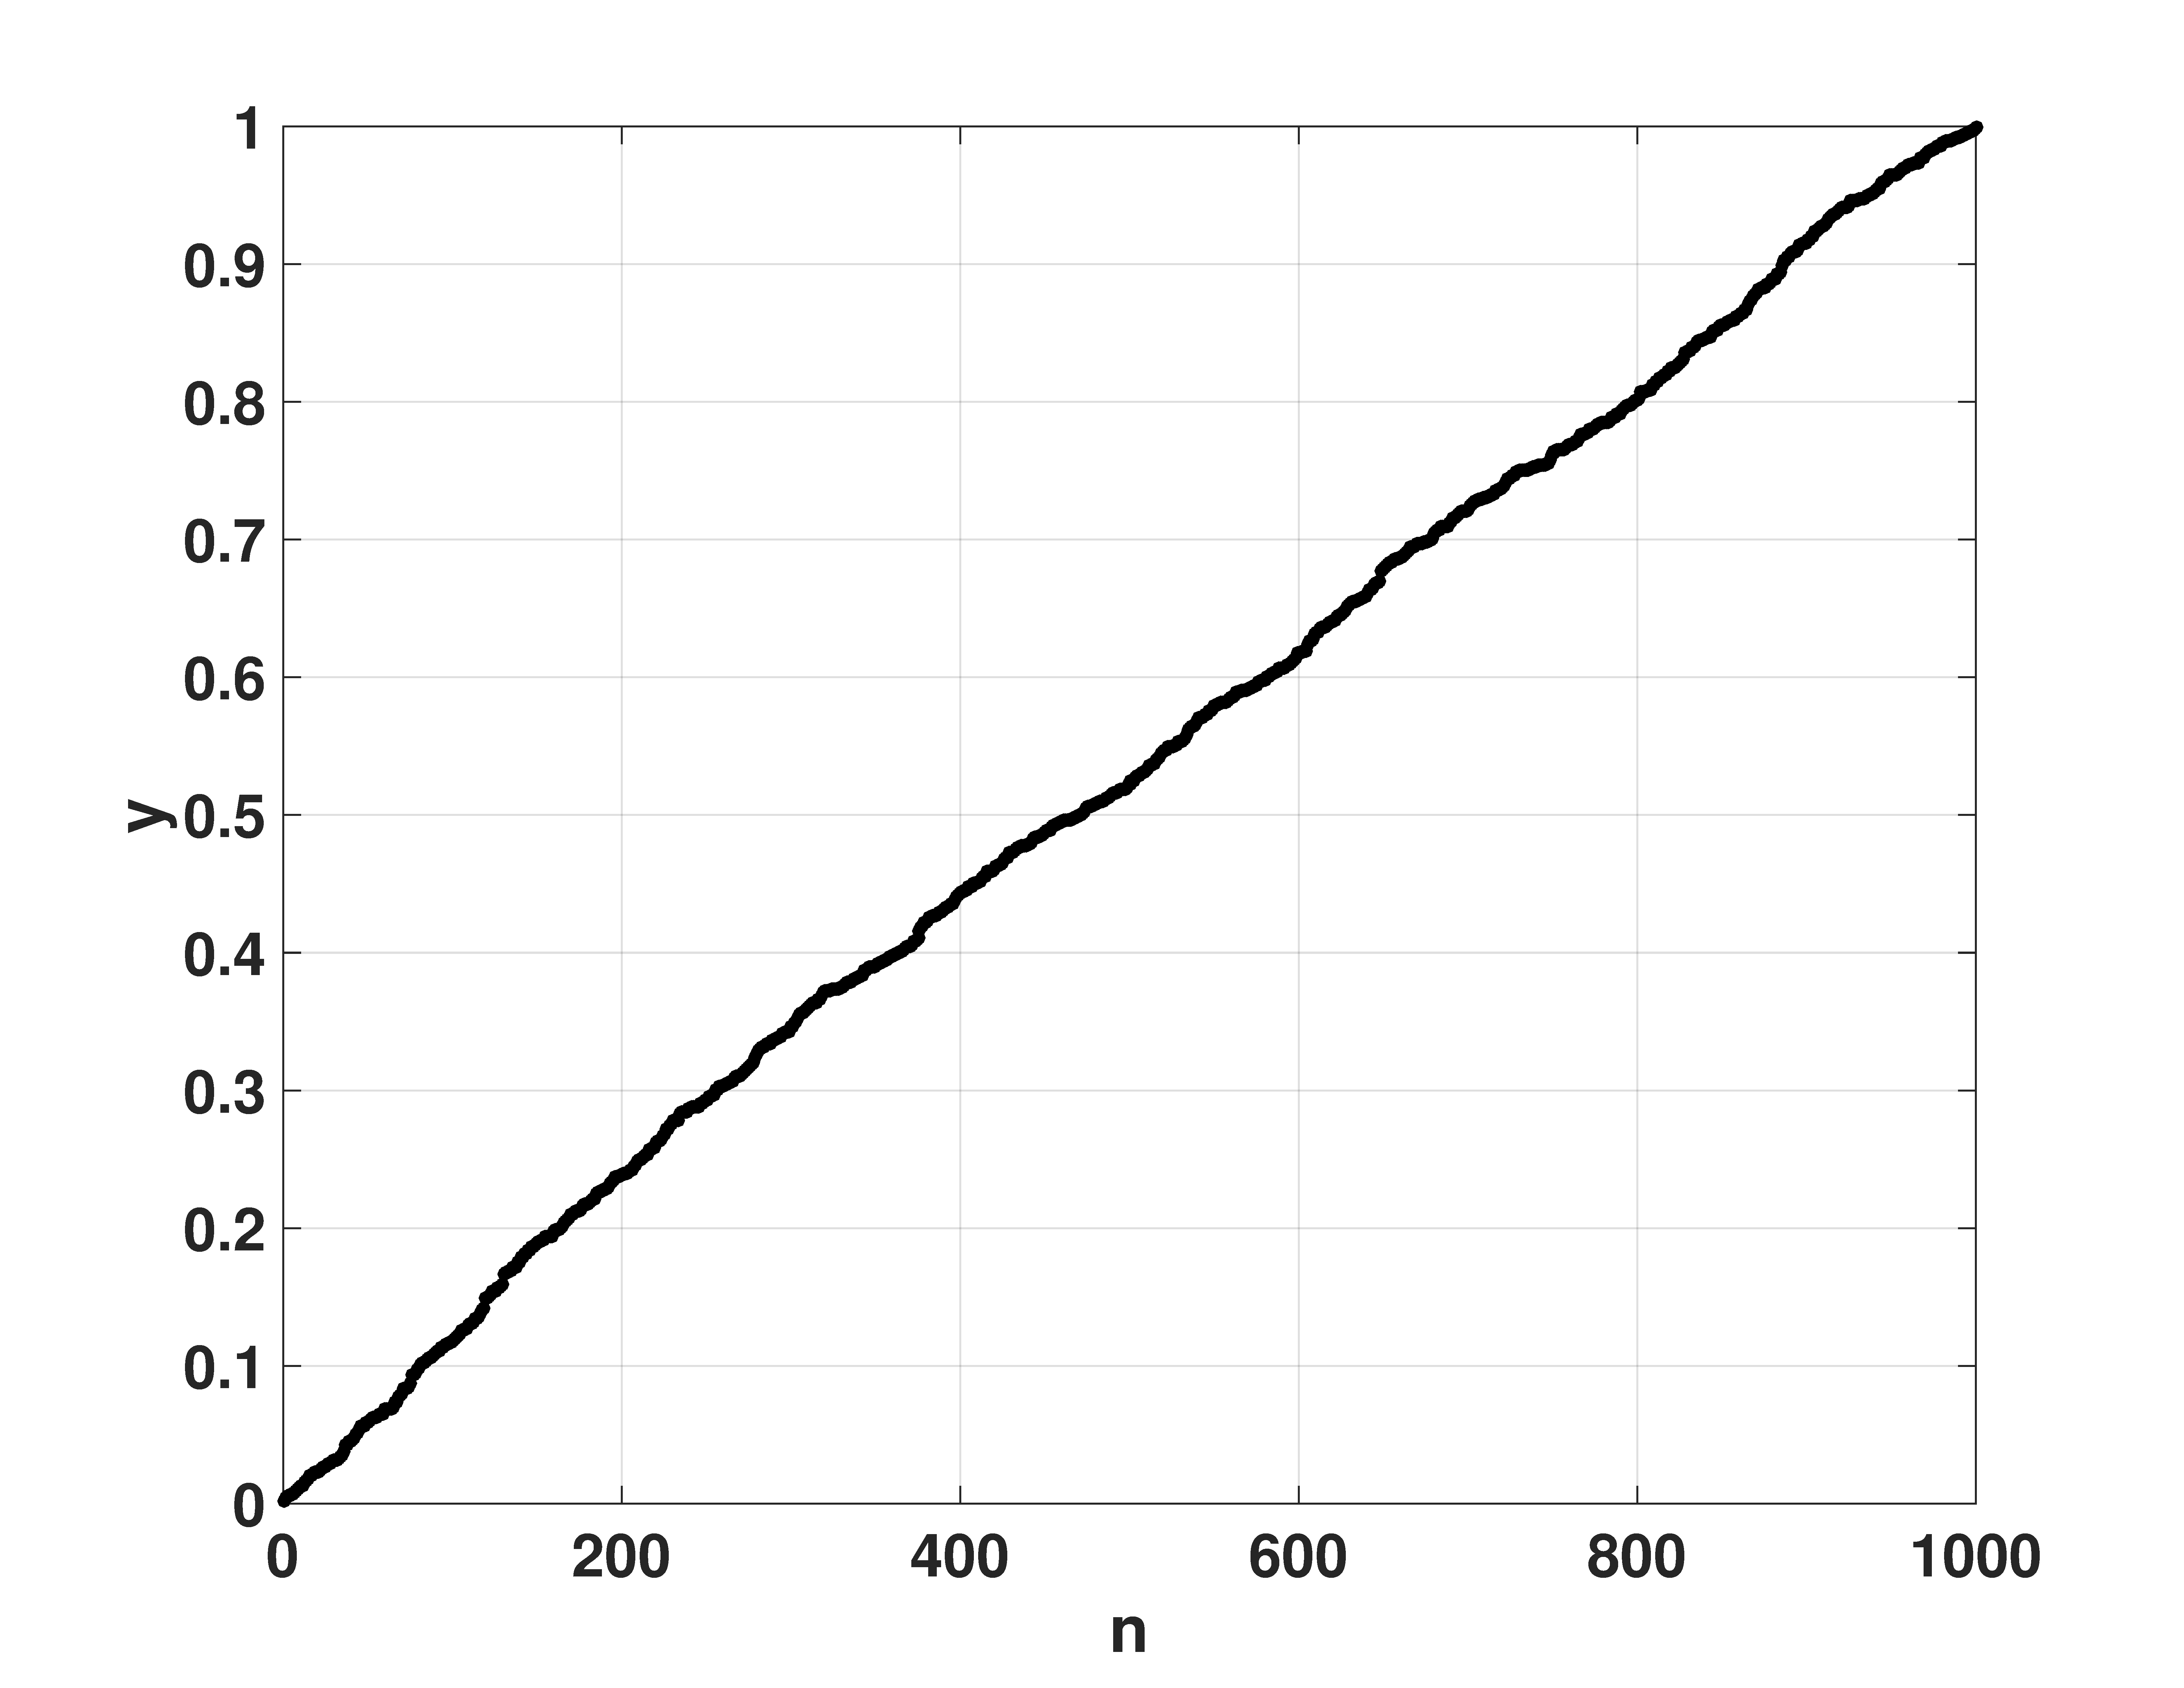
\includegraphics[width=\textwidth]{y}
		\caption{Puntos ordenados}
		\label{subfig:causal_nocausal_y}
	\end{subfigure}
	\begin{subfigure}[t]{0.49\textwidth}
		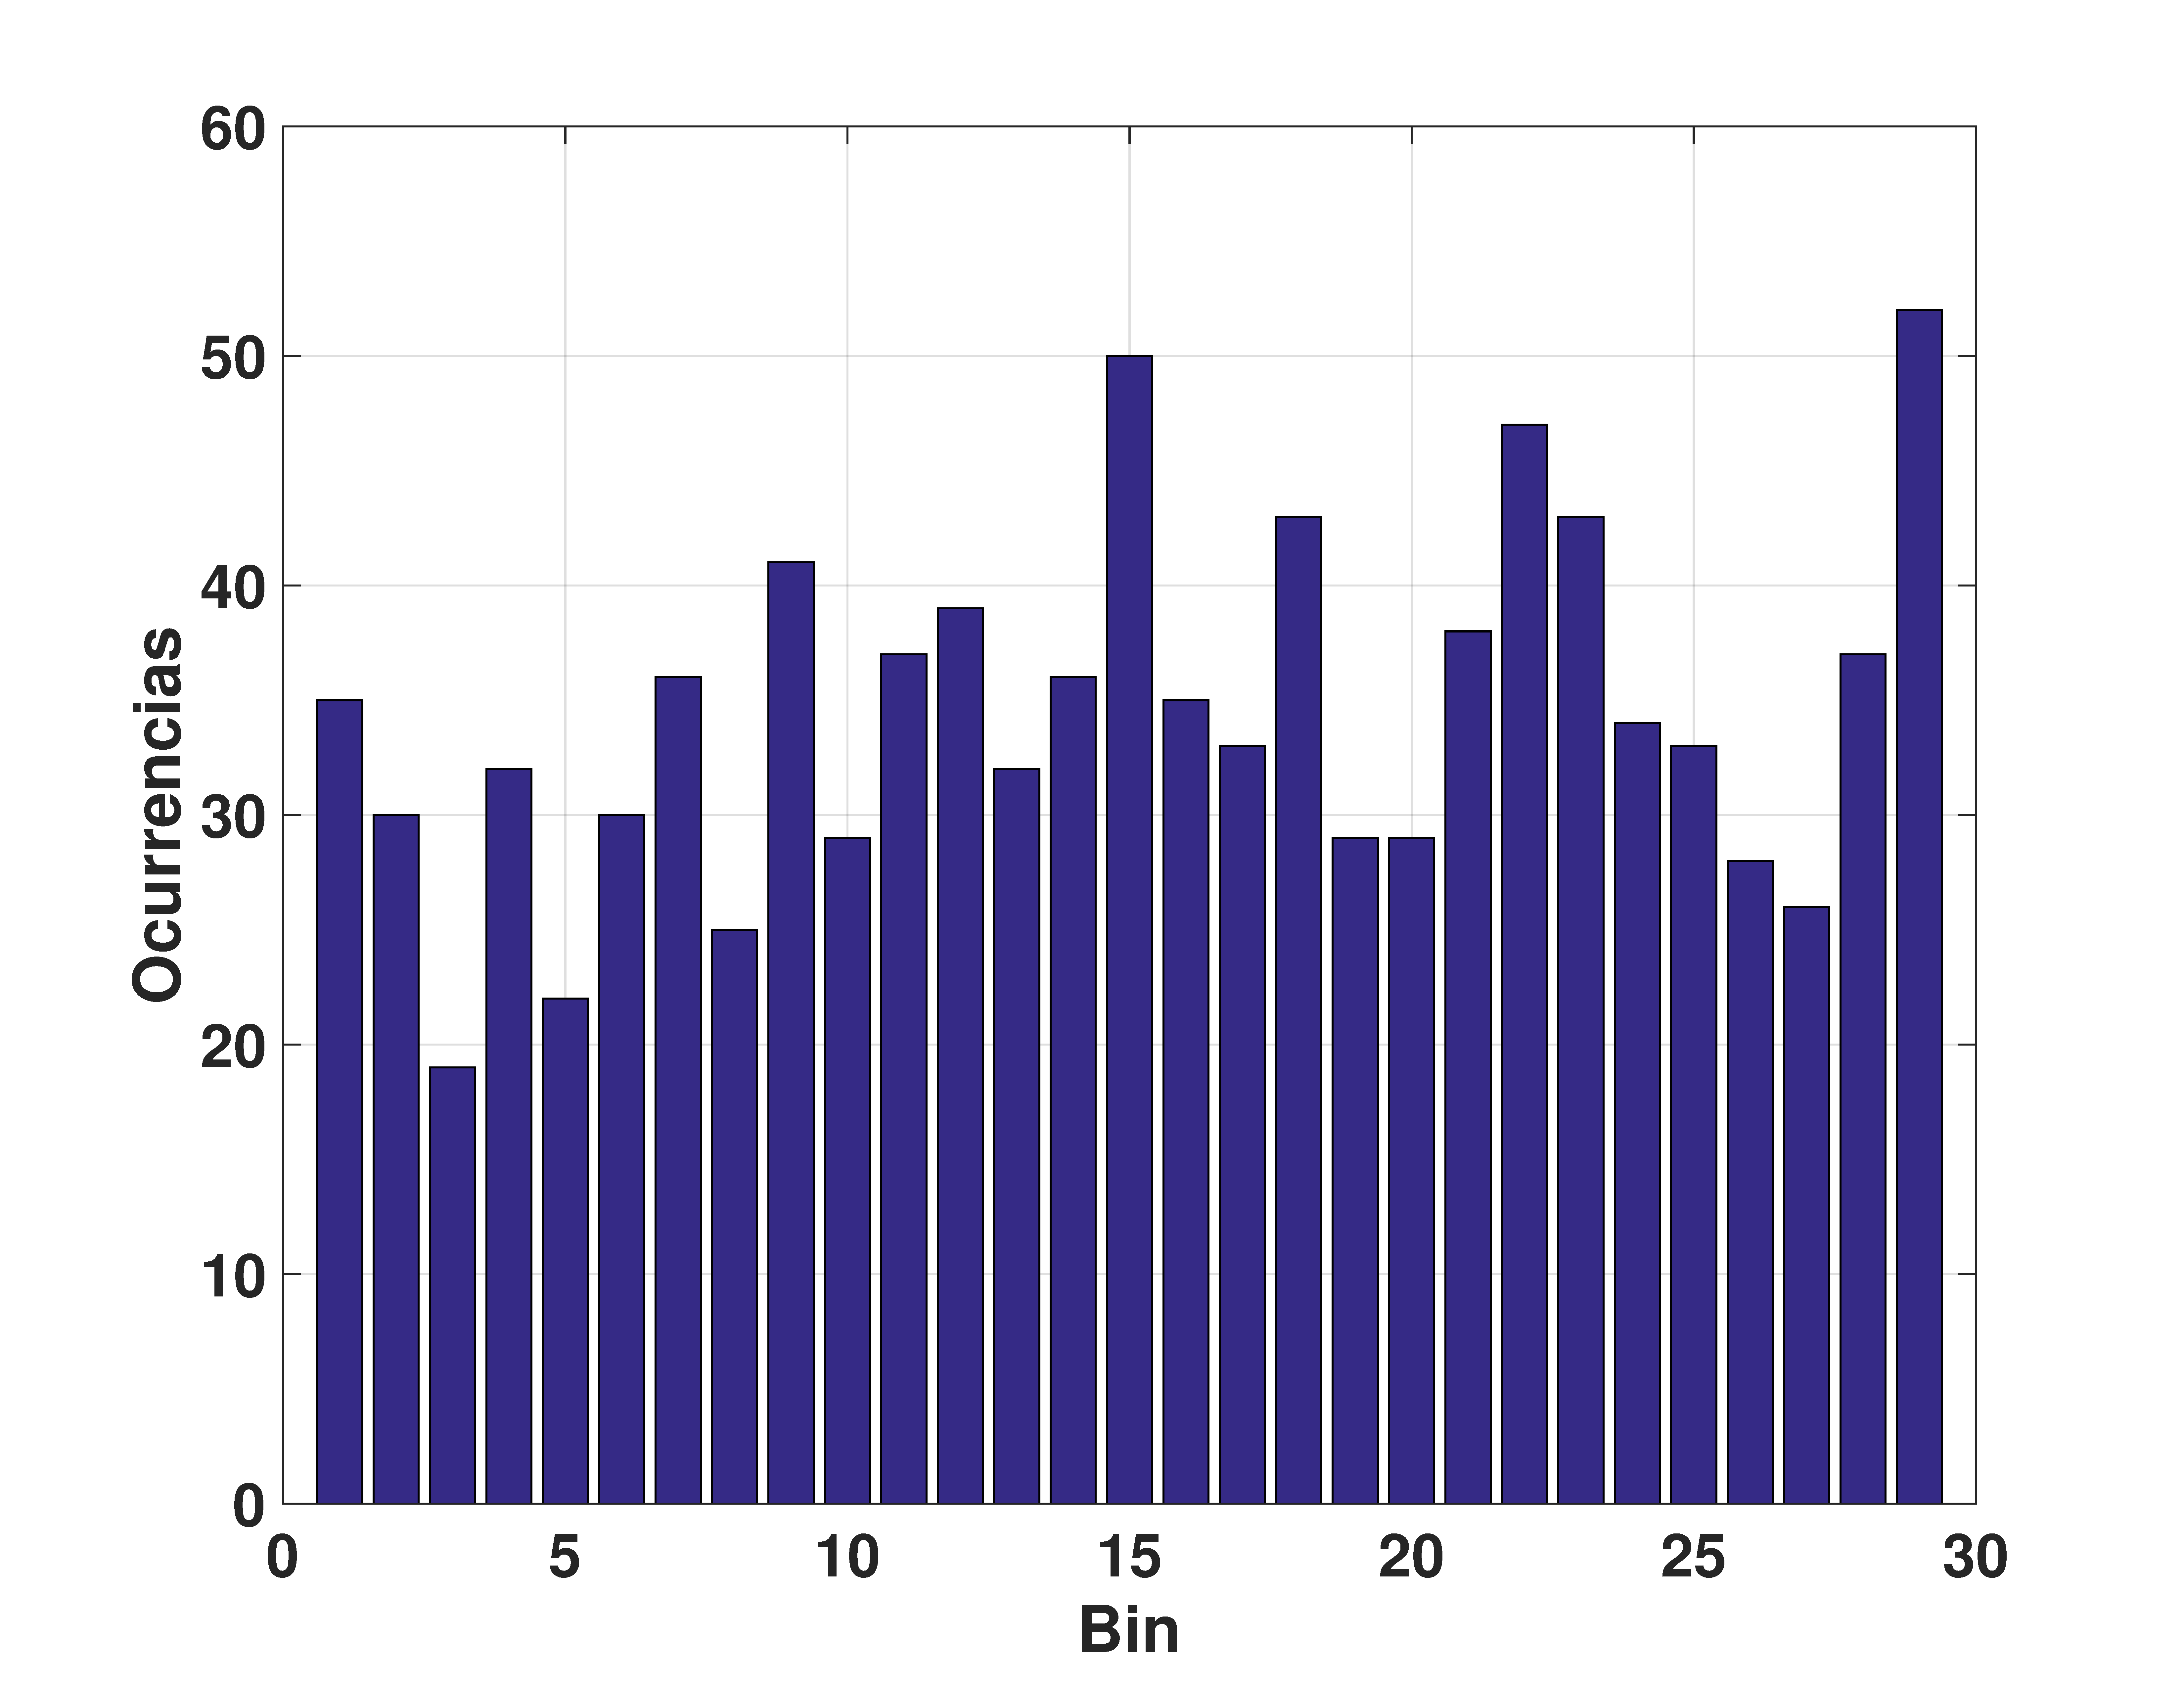
\includegraphics[width=\textwidth]{HistVal_x}
		\caption{Histograma de valores de los puntos sin ordenar}
		\label{subfig:causal_nocausal_HistValx}
	\end{subfigure}
	\begin{subfigure}[t]{0.49\textwidth}
		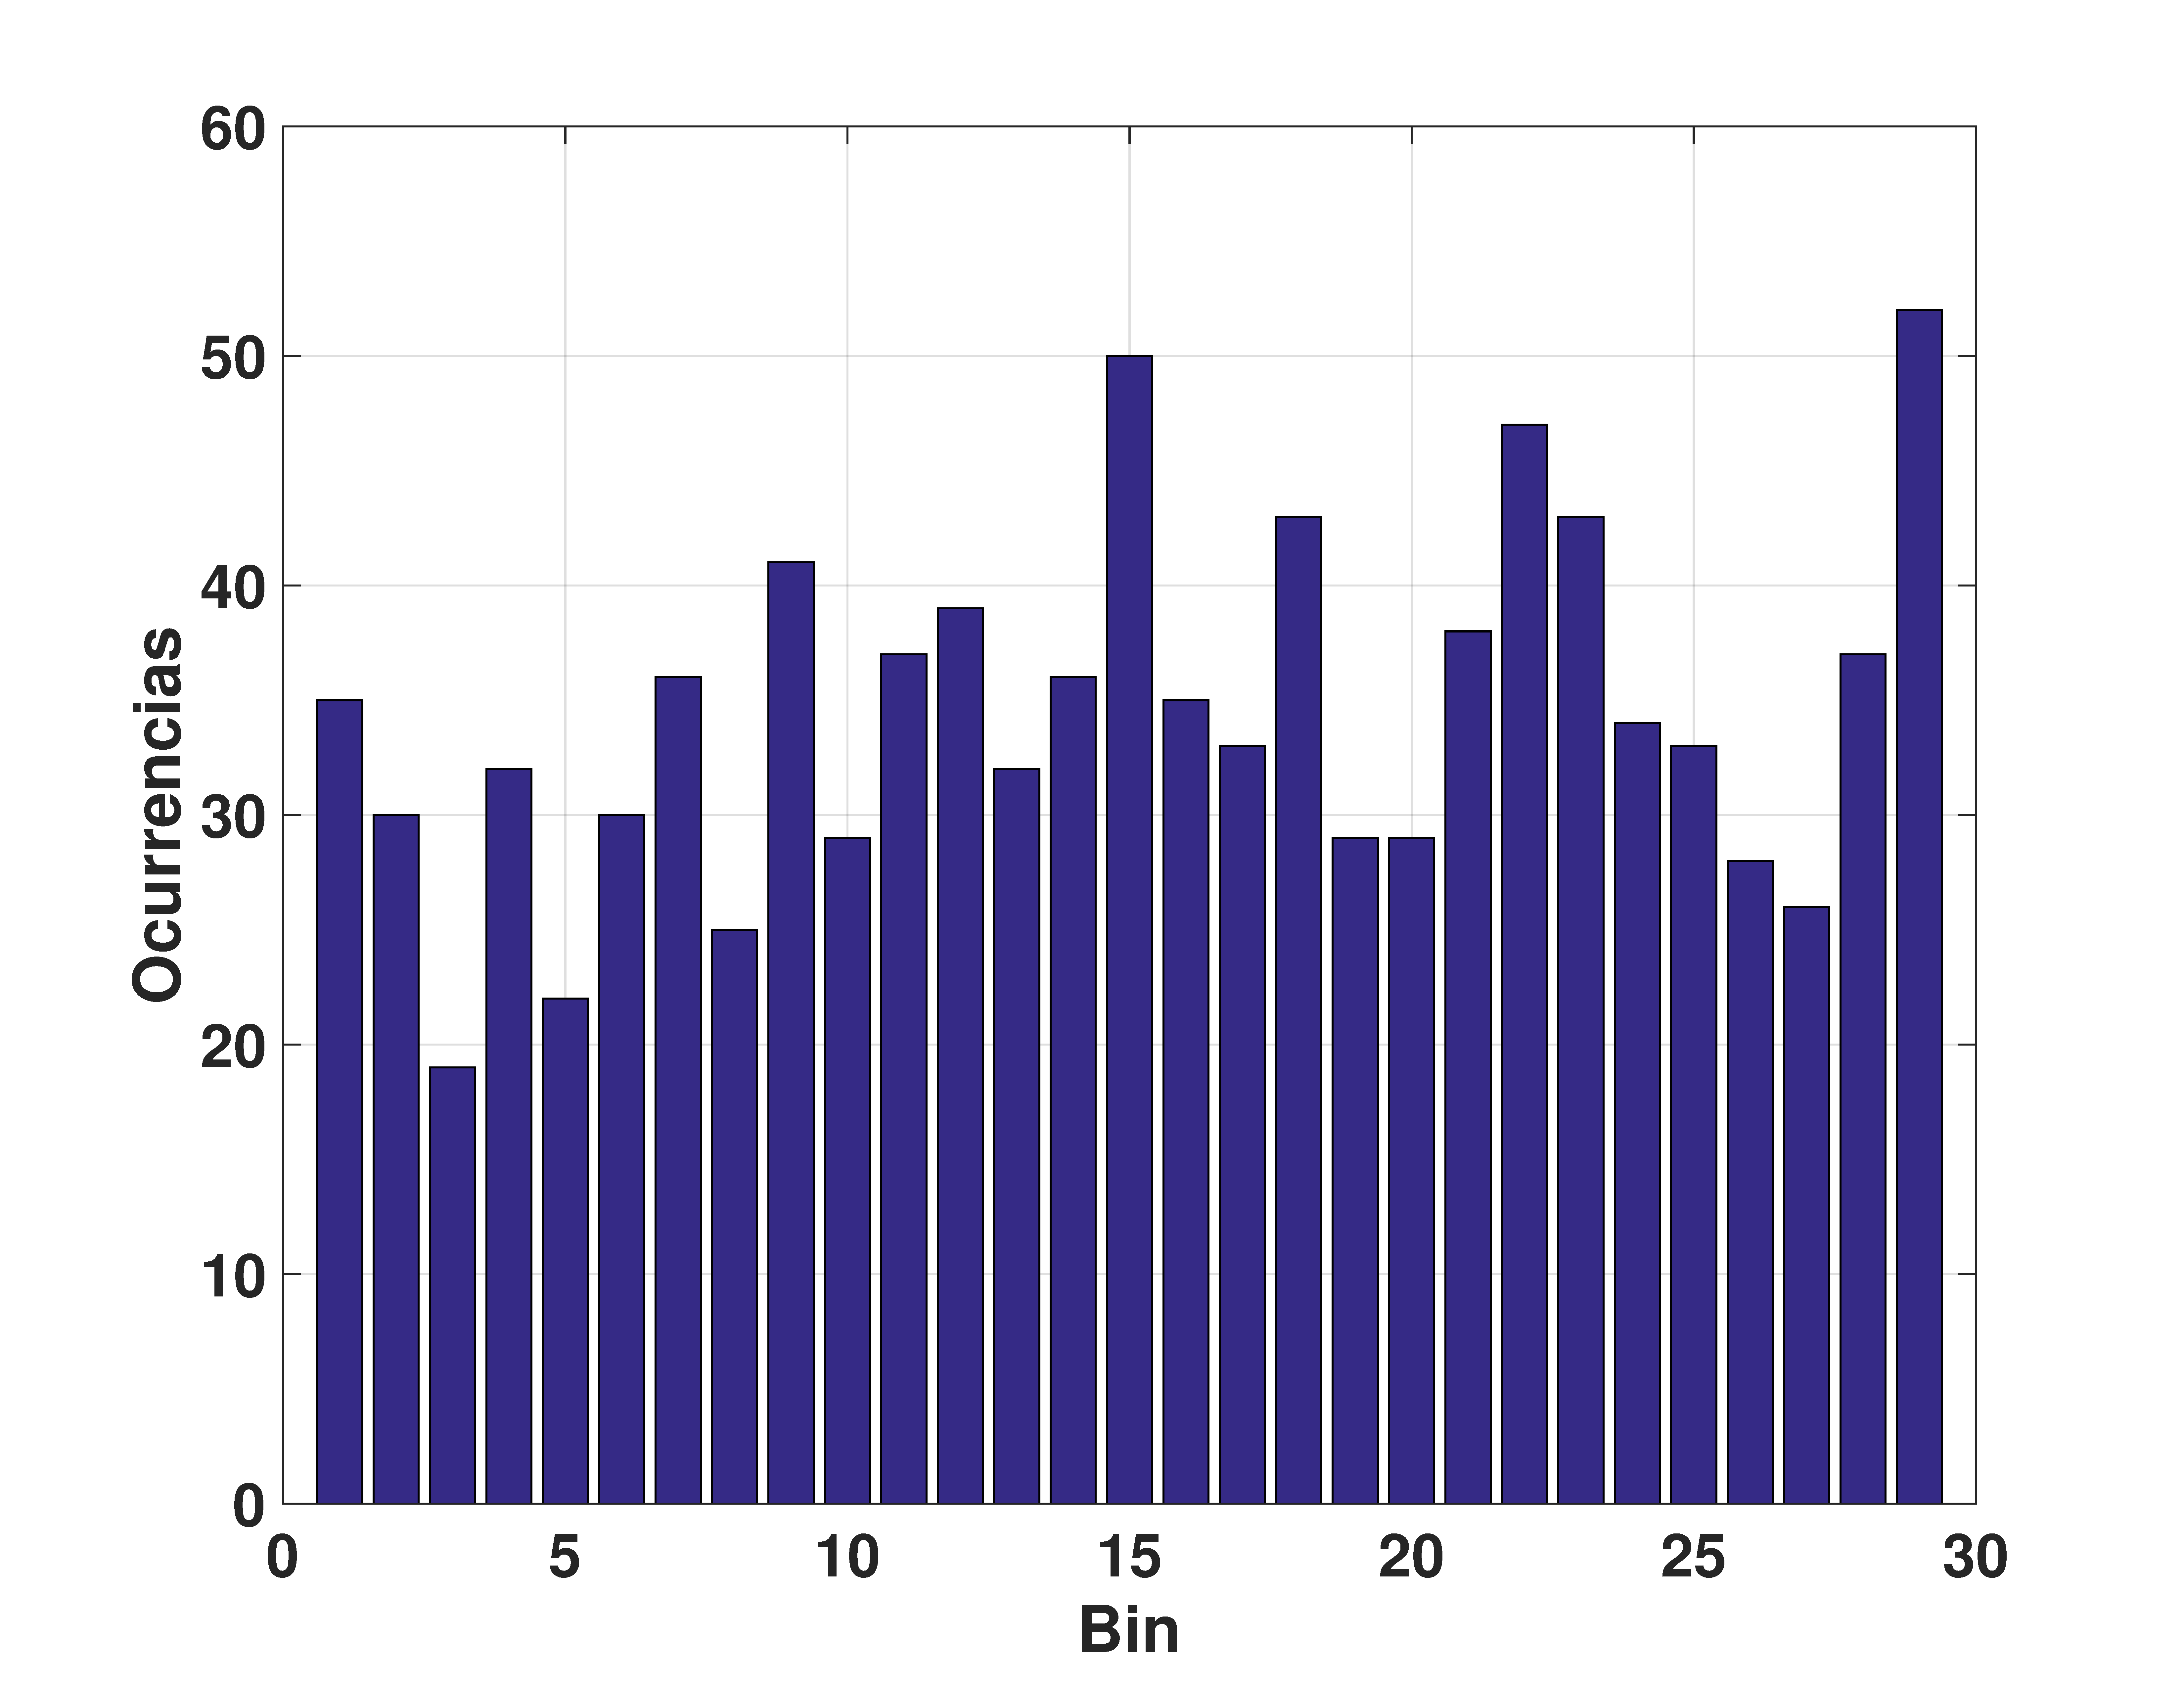
\includegraphics[width=\textwidth]{HistVal_y}
		\caption{Histograma de valores de los puntos ordenados}
		\label{subfig:causal_nocausal_HistValy}
	\end{subfigure}
	\begin{subfigure}[t]{0.49\textwidth}
		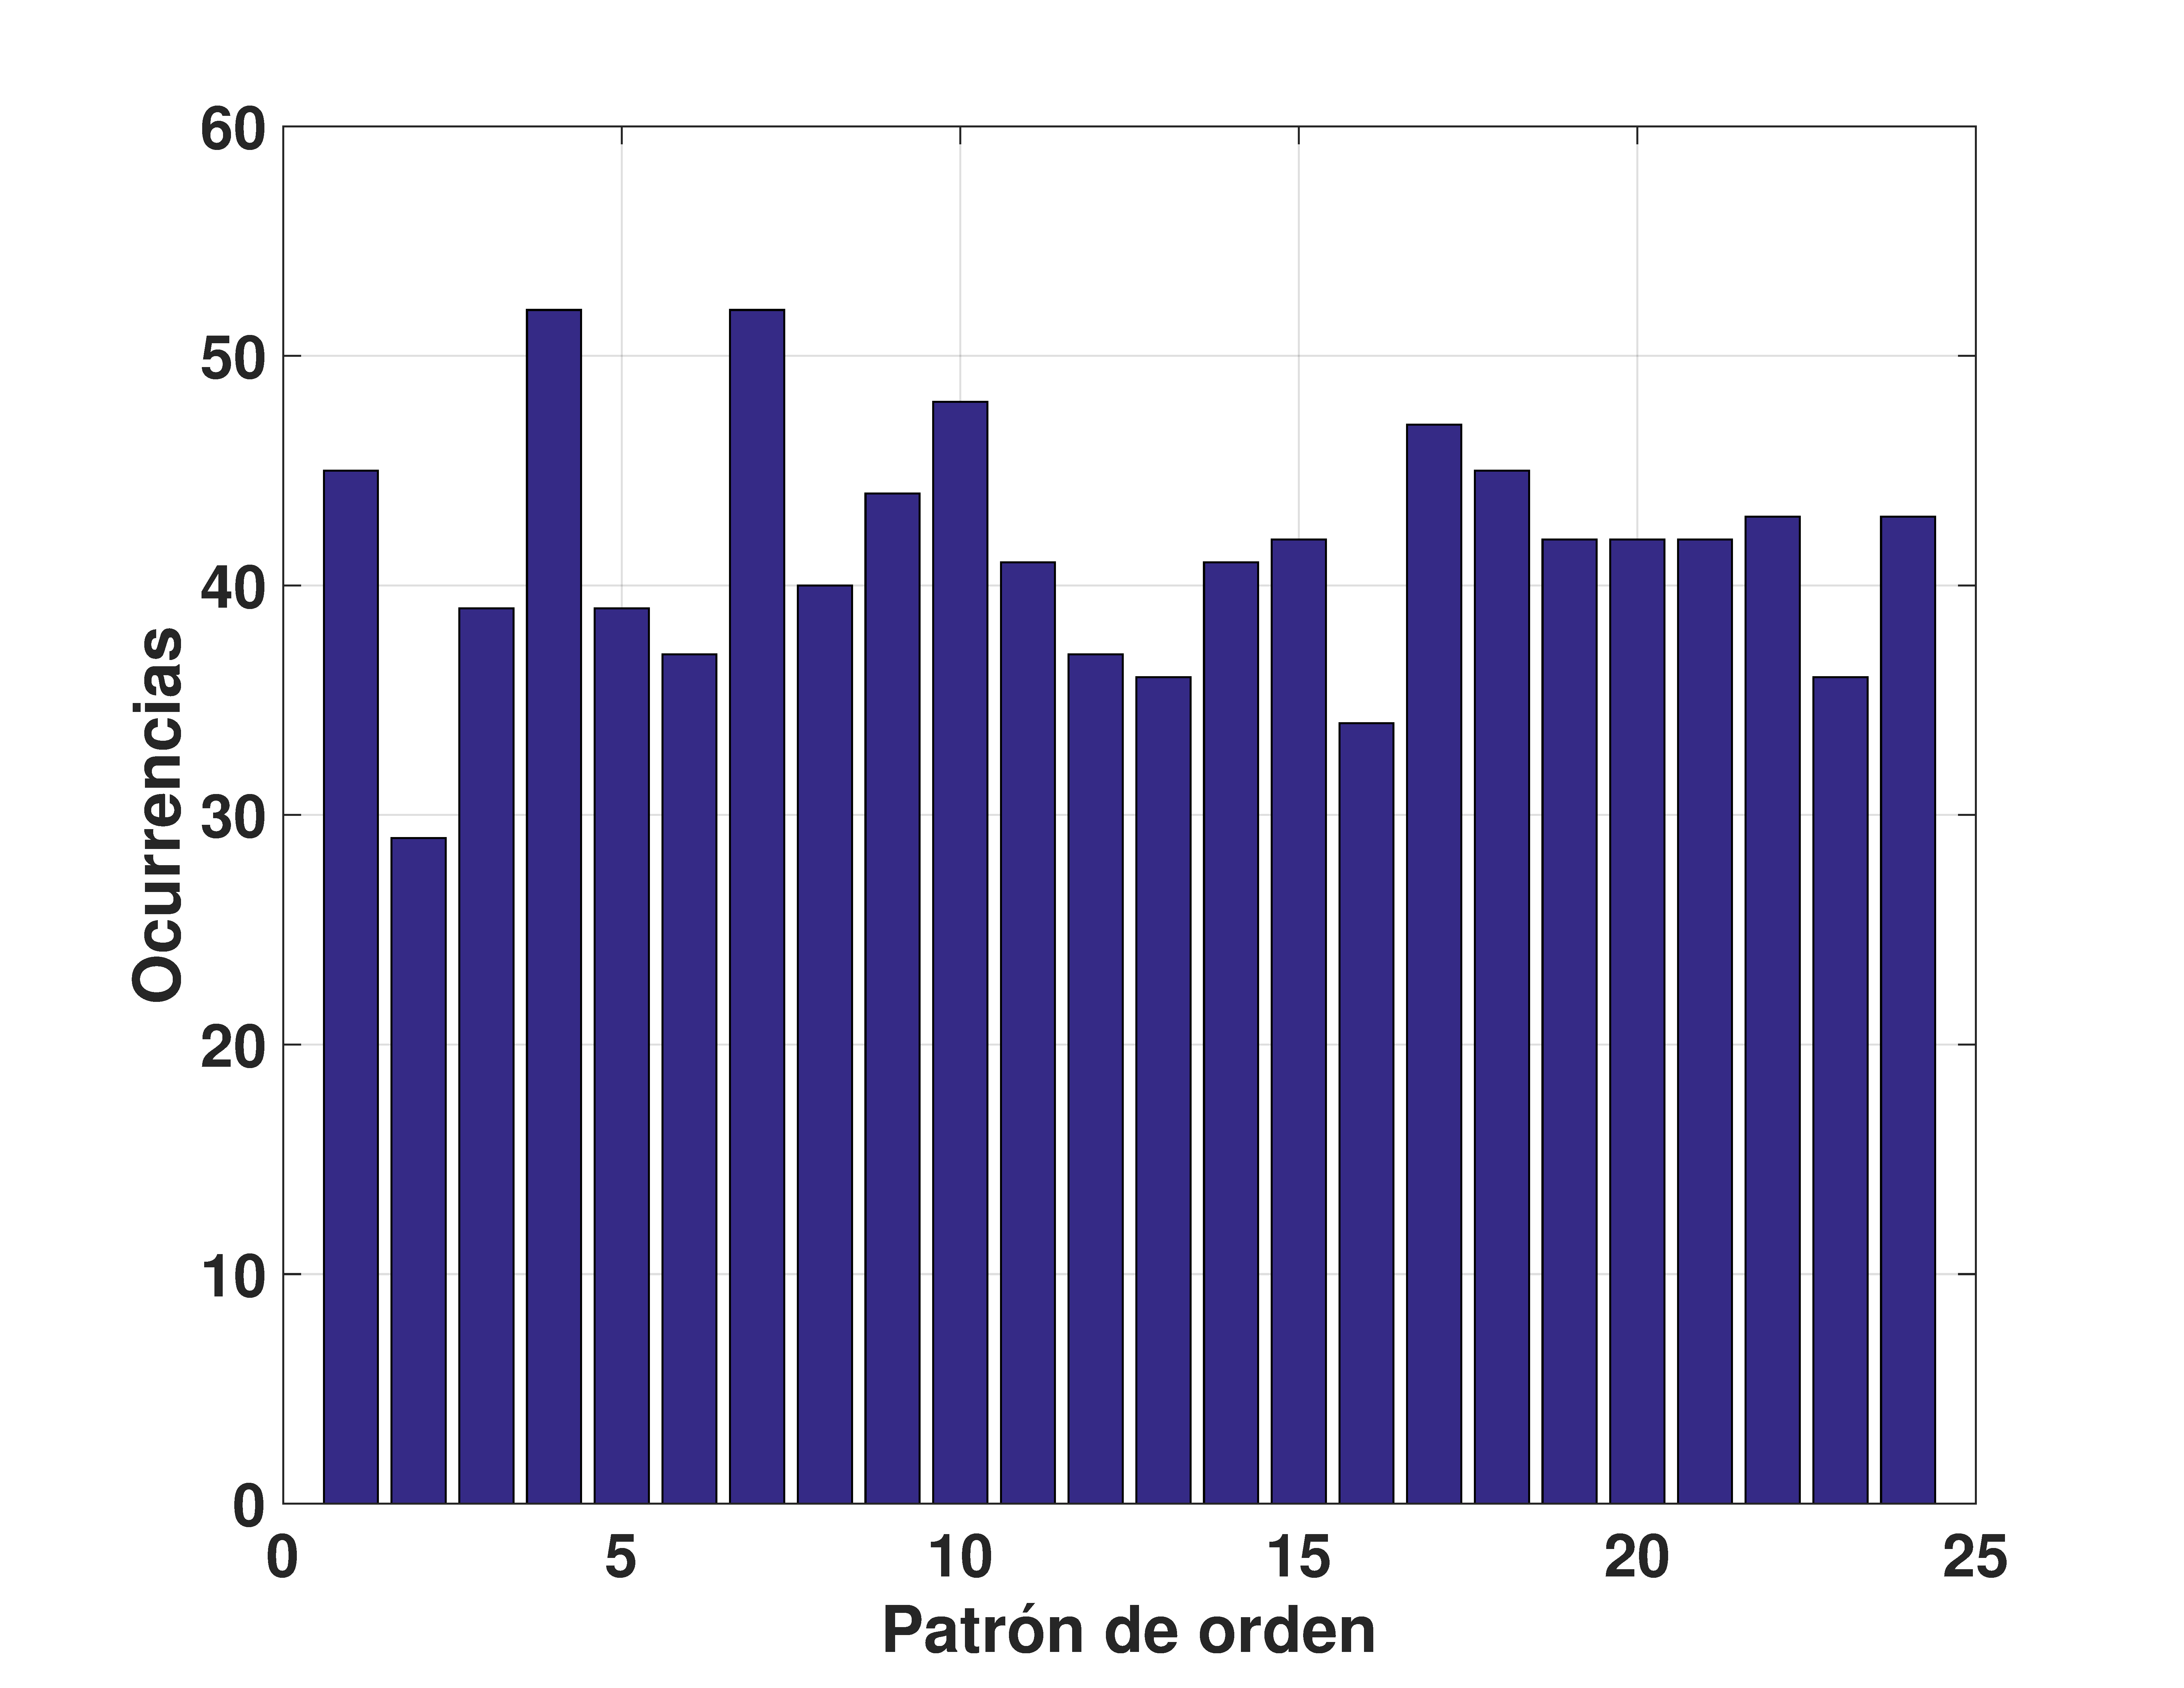
\includegraphics[width=\textwidth]{HistBP_x}
		\caption{Histograma de patrones de orden de los puntos sin ordenar}
		\label{subfig:causal_nocausal_HistBPx}
	\end{subfigure}
	\begin{subfigure}[t]{0.49\textwidth}
		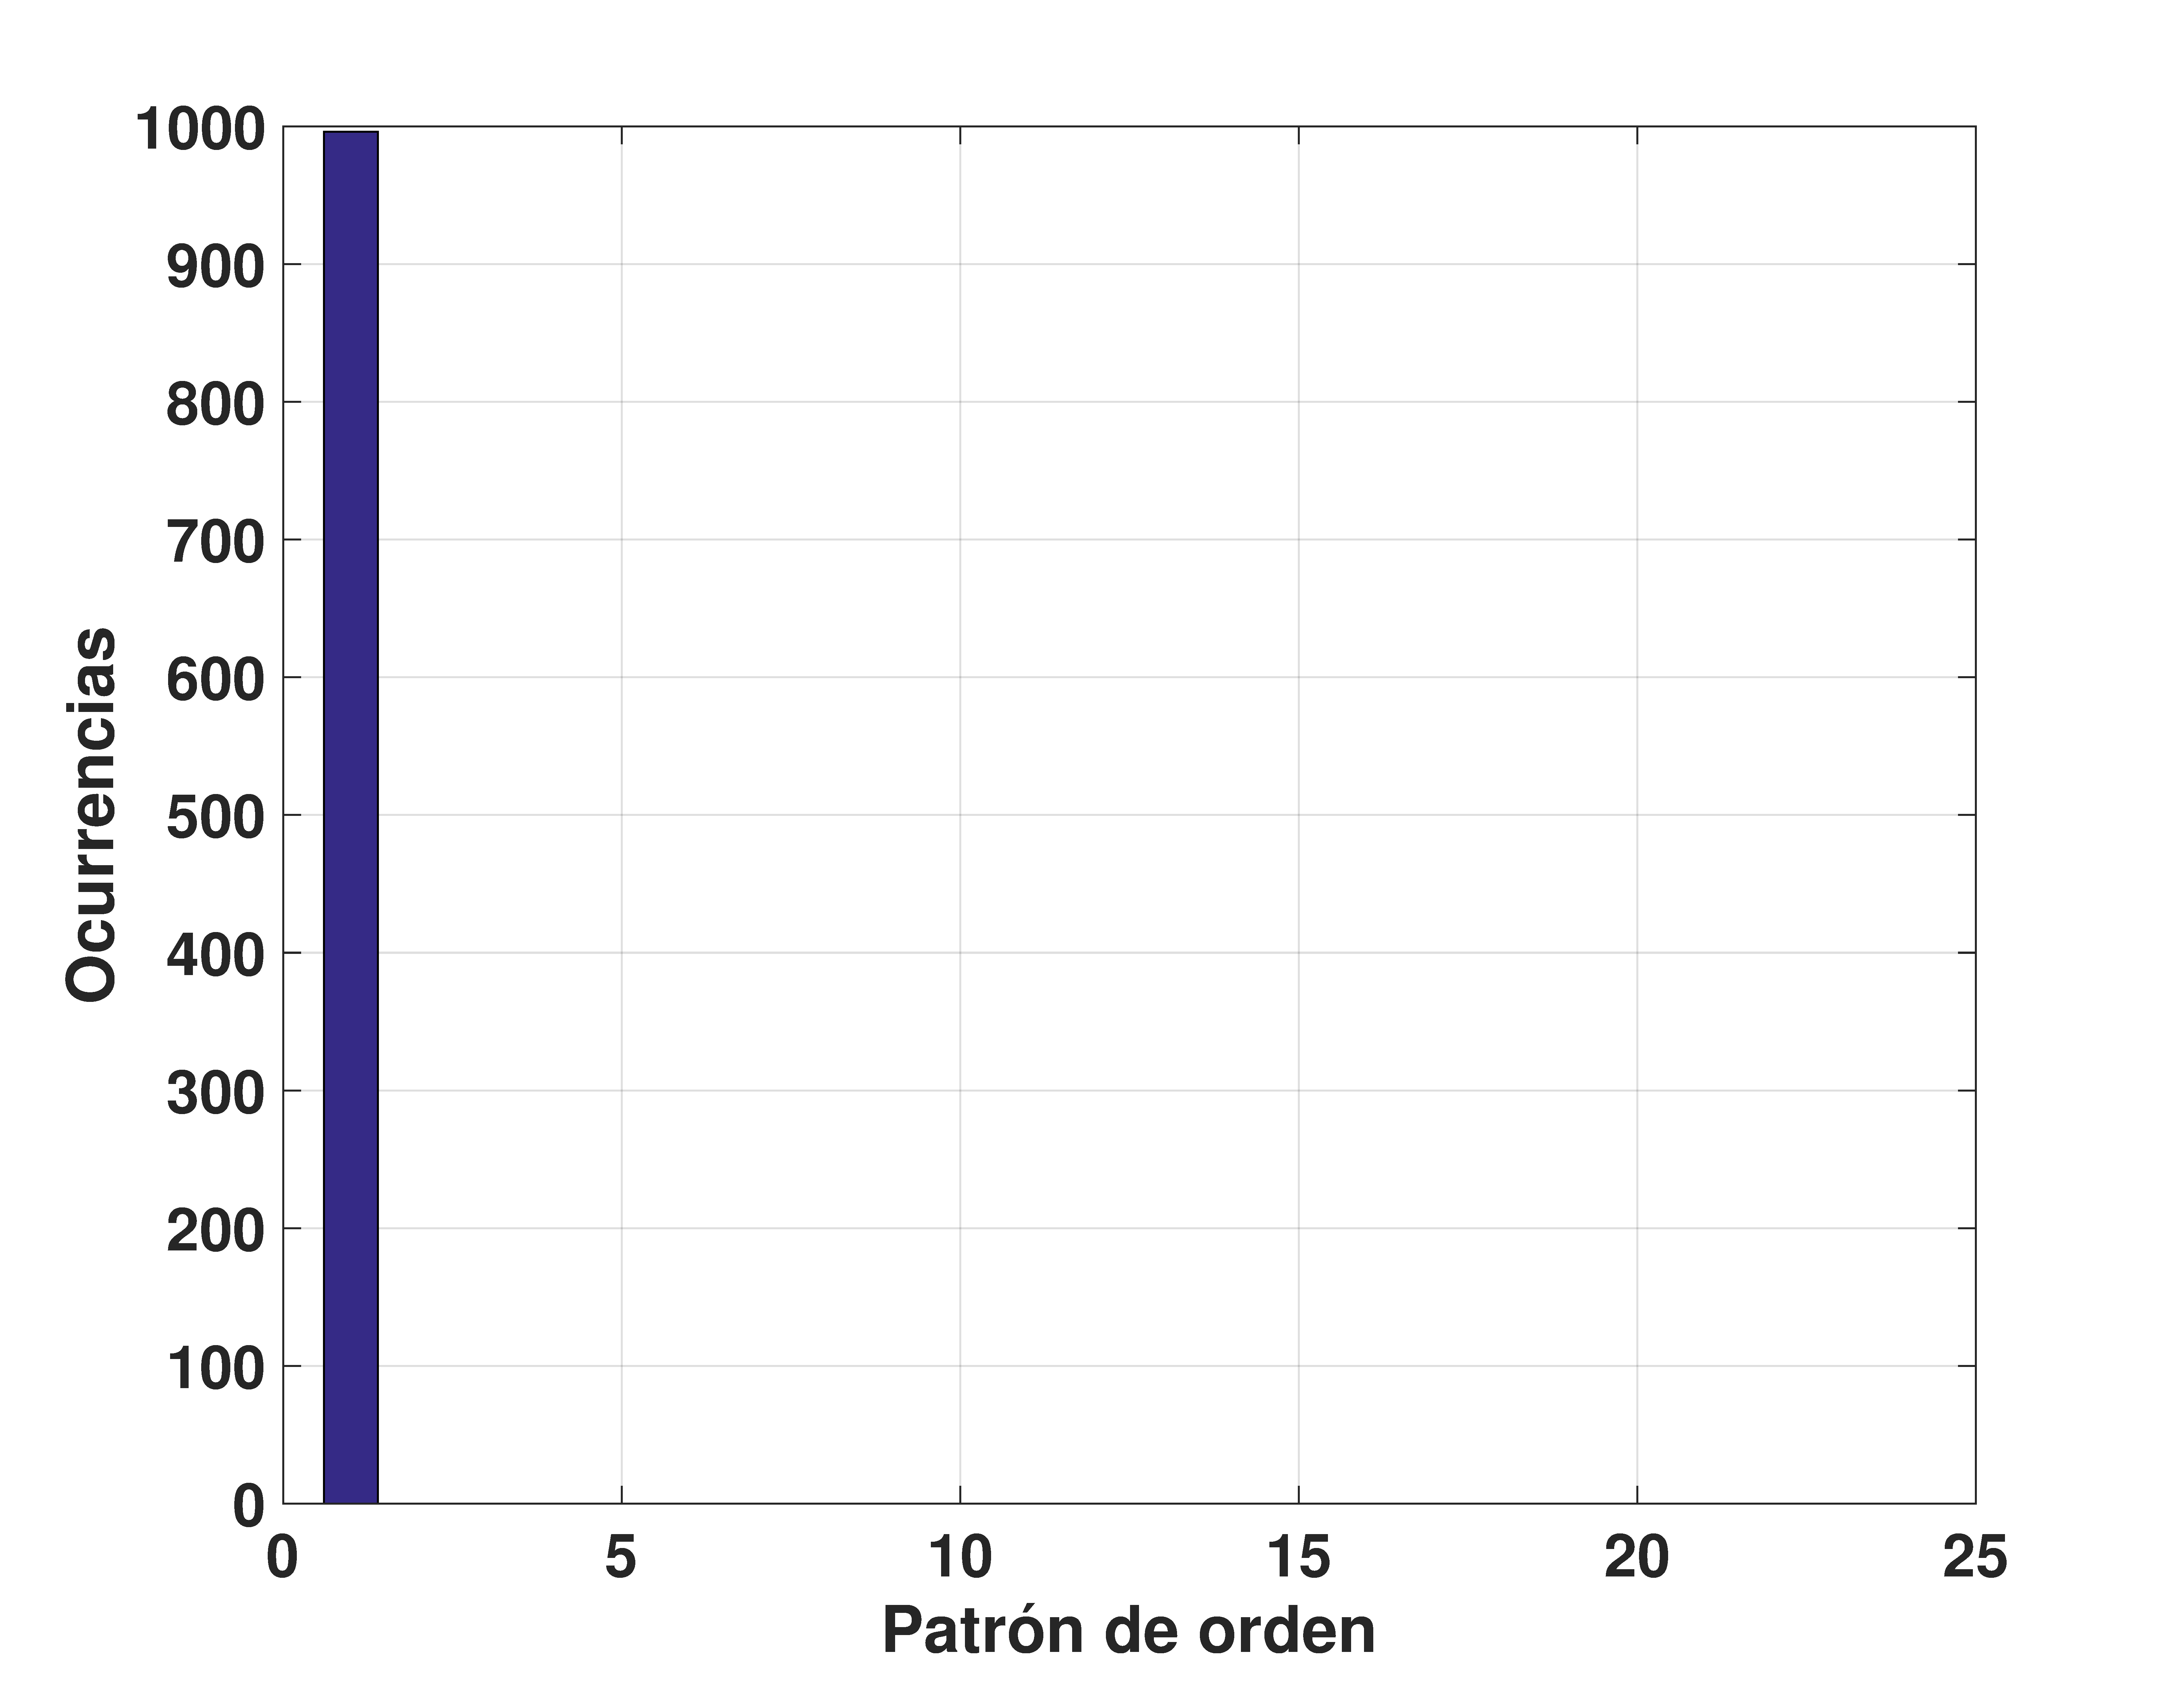
\includegraphics[width=\textwidth]{HistBP_y}
		\caption{Histograma de patrones de orden de los puntos ordenados}
		\label{subfig:causal_nocausal_HistBPy}
	\end{subfigure}
	\caption{Comparación entre histogramas causal y no causal}\label{fig:causal_nocausal}
\end{figure}

Recientemente, la entropía de permutación se amplió para incorporar también información de amplitud.
Ponderar las probabilidades de patrones individuales de acuerdo a su varianza mitiga los problemas potenciales con respecto a los patrones de "alto ruido, baja señal", porque los patrones de baja varianza que están fuertemente afectados por el ruido se ponderan en las distribuciones de patrones ordinales ponderados resultantes.
Por lo tanto, una posible desventaja de las estadísticas de los patrones ordinales, es decir, la pérdida de información de amplitud, se puede abordar mediante la introducción de pesos con el fin de obtener una "entropía de permutación ponderada (WPE)" \cite{Fadlallah2013}.
Los pesos no normalizados se calculan para cada ventana temporal para la serie de tiempo $X$, tal que
\begin{equation}
\label{WPE_weigth}
w_j~=~\frac{1}{D}\sum_{k=1}^{D} \left(x_{j+k-1}-\bar{X_j^D}\right)^2.
\end{equation}
En la ecuación anterior $x_{j+k-1}-\bar{X_j^D}$ denota la media aritmética del actual vector de embedding de longitud $D$ y su varianza $w_j$ se utiliza entonces para ponderar las frecuencias relativas de cada patrón ordinal $p_j$.
Originalmente, se propuso esta técnica para discriminar patrones sumergidos en un bajo nivel de ruido.
Nosotros también aprovechamos el hecho de que los puntos fijos no se computan en el WPE.

Al calcular la entropía de Shannon normalizada $H$ y la complejidad estadística $C$ de estas PDFs, y los valores obtenidos se denotan como:
\begin{itemize}
	\item $H_{hist}$, es la entropía de Shannon normalizada aplicada a una PDF no causal $P_{hist}$
	\item $H_{BP}$, es la entropía de Shannon normalizada aplicada a una PDF causal $P_{BP}$
	\item $H_{BPW}$,es la entropía de Shannon normalizada aplicada a una PDF causal con contribuciones de aplitud $P_{BPW}$
	\item $C_{BP}$, es la complejidad estadística normalizada aplicada a una PDF causal $P_{BP}$
	\item $C_{BPW}$, es la complejidad estadística normalizada aplicada a una PDF causal con contribuciones de amplitud $P_{BPW} $
\end{itemize}

\subsection{Planos deoble entropía y entropía-complejidad}

Una visualización particularmente útil de los cuantificadores de la Teoría de la Información es su yuxtaposición en los gráficos bidimensionales.
Se definen cuatro planos de información:
\begin{enumerate}
	\item Entropía causal vs. entropía no-causal, $H_{BP} \times H_{hist}$
	\item Entropía causal con contribución de amplitudes vs. entropía no-causal, $H_{BPW} \times H_{hist}$
	\item Complejidad causal vs. entropía causal, $C_{BP} \times H_{BP}$
	\item Complejidad causal con contribución de amplitudes vs. entropía causal con contribución de amplitudes, $C_{BPW} \times H_{BPW}$
\end{enumerate}

Estas herramientas de diagnóstico demostraron ser particularmente eficientes para distinguir entre el caos determinista y la naturaleza estocástica de una serie de tiempo ya que los cuantificadores de permutación tienen comportamientos distintos para diferentes tipos de procesos.

En la Fig. \ref{fig: HH} se muestran los planos $H_ {BP} \times H_{hist}$ y $H_{BPW} \times H_{hist}$ colapsados en un mismo plano.
En este plano un valor más alto en cualquiera de las entropías, $H_{BP}$, $H_{BPW}$ o $H_{hist}$, implica una mayor uniformidad de la PDF implicada.
El punto $(1, 1)$ representa el caso ideal con histograma uniforme y distribución uniforme de los patrones de orden.
Mostramos algunos puntos relevantes como ejemplo.

El ruido aleatorio blanco ideal con distribución uniforme da un punto en $(H_{hist}, H_{BP}) = (1, 1)$ representado por un círculo azul, un círculo rojo en la misma posición muestra los resultados cuando se incluyen las contribuciones de amplitud $(H_{hist}, H_{BPW}) = (1, 1)$.
Si ordenamos el vector ideal con distribución uniforme de forma ascendente, los puntos resultantes se muestran con un cuadrado azul $(H_{hist}, H_{BP}) = (1, 0)$ y un cuadrado rojo $(H_{hist}, H_{BPW}) = (1, 0)$, este ejemplo ilustra la complementariedad de $H_{hist}$ y $H_{BP}$.

Las estrellas azules y rojas muestran $(H_{hist}, H_{BP})$ y $ (H_{hist}, H_{BPW})$ respectivamente aplicadas a una señal de diente de sierra.
Los valores están perfectamente distribuidos en todos los intervalos, pero sólo aparecen unos pocos patrones de orden, esto explica el alto $H_ {hist}$ y bajo $H_ {BP}$.
La frecuencia de aparición de patrones de baja amplitud es mayor que los patrones de alta amplitud, entonces la PDF con contribuciones de amplitud es más uniforme y $H_ {BPW}$ es un poco más alto que $H_ {BP}$.
Cuando la señal de diente de sierra está contaminada con ruido blanco, se incrementan $H_ {BP}$ y $H_ {BPW}$ como se muestra con triángulos azules y rojos.
Es evidente que aparecen nuevos patrones de orden y tanto $H_{BP}$ como $H_{BPW}$ muestran valores más altos que los casos no contaminados, sin embargo el incremento de $H_{BPW}$ es menor que $H_{BP}$ mostrando que la técnica de registrar contribuciones de amplitud añade alguna inmunidad al ruido.

Finalmente, se evaluaron los cuantificadores de una secuencia de un mapa logístico que converge a un punto fijo, en todos los casos la longitud del vector de datos permanece constante y la longitud de transitorio es variable.
Los resultados obtenidos sin las contribuciones de amplitud se representan en puntos azules, convergen a $(H_{hist}, H_{BP}) = (0, 0)$ a medida que la longitud de transitorio se hace más corta, sin embargo $H_{BPW}$ (puntos rojos) permanece constante para todos los casos.
El último punto en $(H_{hist}, H_{BP}) = (0, 0)$ corresponde a un vector de ceros, en este caso el histograma de patrones de orden con contribuciones de amplitud es también un vector nulo y $H_{BPW}$ no se puede calcular.
A través de este último ejemplo, mostramos que la convergencia a un punto fijo puede ser detectada por la información conjunta de $H_{BP}$ y $H_{BPW}$.

En la figura \ref{fig:HC} se muestra el plano causal $H_{BP} \times C_{BP}$.
Podemos ver que no toda la región $0 < H_{BP} < 1$, $0 < C_{BP} < 1$ es alcanzable, de hecho, para cualquier PDF los pares $(H, C)$ de valores posibles caen entre dos curvas extremas en el plano $H_{BP} \times C_{BP}$ \ cite {Anteneodo1996}.
Los mapas caóticos tienen entropía intermedia $H_{BP}$, mientras que su complejidad $C_{BP}$ alcanza valores mayores, muy cercanos a los del límite de complejidad superior \cite{Rosso2007, Olivares2012}.
Para procesos regulares, la entropía y la complejidad tienen valores pequeños, cercanos a cero.
Los procesos estocásticos no correlacionados se ubican en la localización planar asociada con $H_{BP}$ cerca de uno y $C_{BP}$ cerca de cero.
Los sistemas aleatorios ideales que tienen un Bandt \& Pompe PDF uniforme, están representados por el punto $(1,0)$ \ cite{Gonzalez2005} y una PDF tipo delta corresponde al punto $(0,0)$.

En la figura \ref{fig:HC} mostramos $H_{BP} \times C_{BP}$ con y sin contribuciones de amplitud.
Se muestran los mismos puntos de muestra para ilustrar las posiciones planas para diferentes vectores de datos.

En ambos planos de información $H_ {BP} \times H_ {hist}$ en la Fig. \ref{fig:HH} y $H_{BP} \times C_{BP}$ en Fig. \ref{fig:HC}, los datos estocásticos, caóticos y deterministas están claramente localizados en diferentes posiciones planares.

\begin{figure}[htpb]
	\centering	
	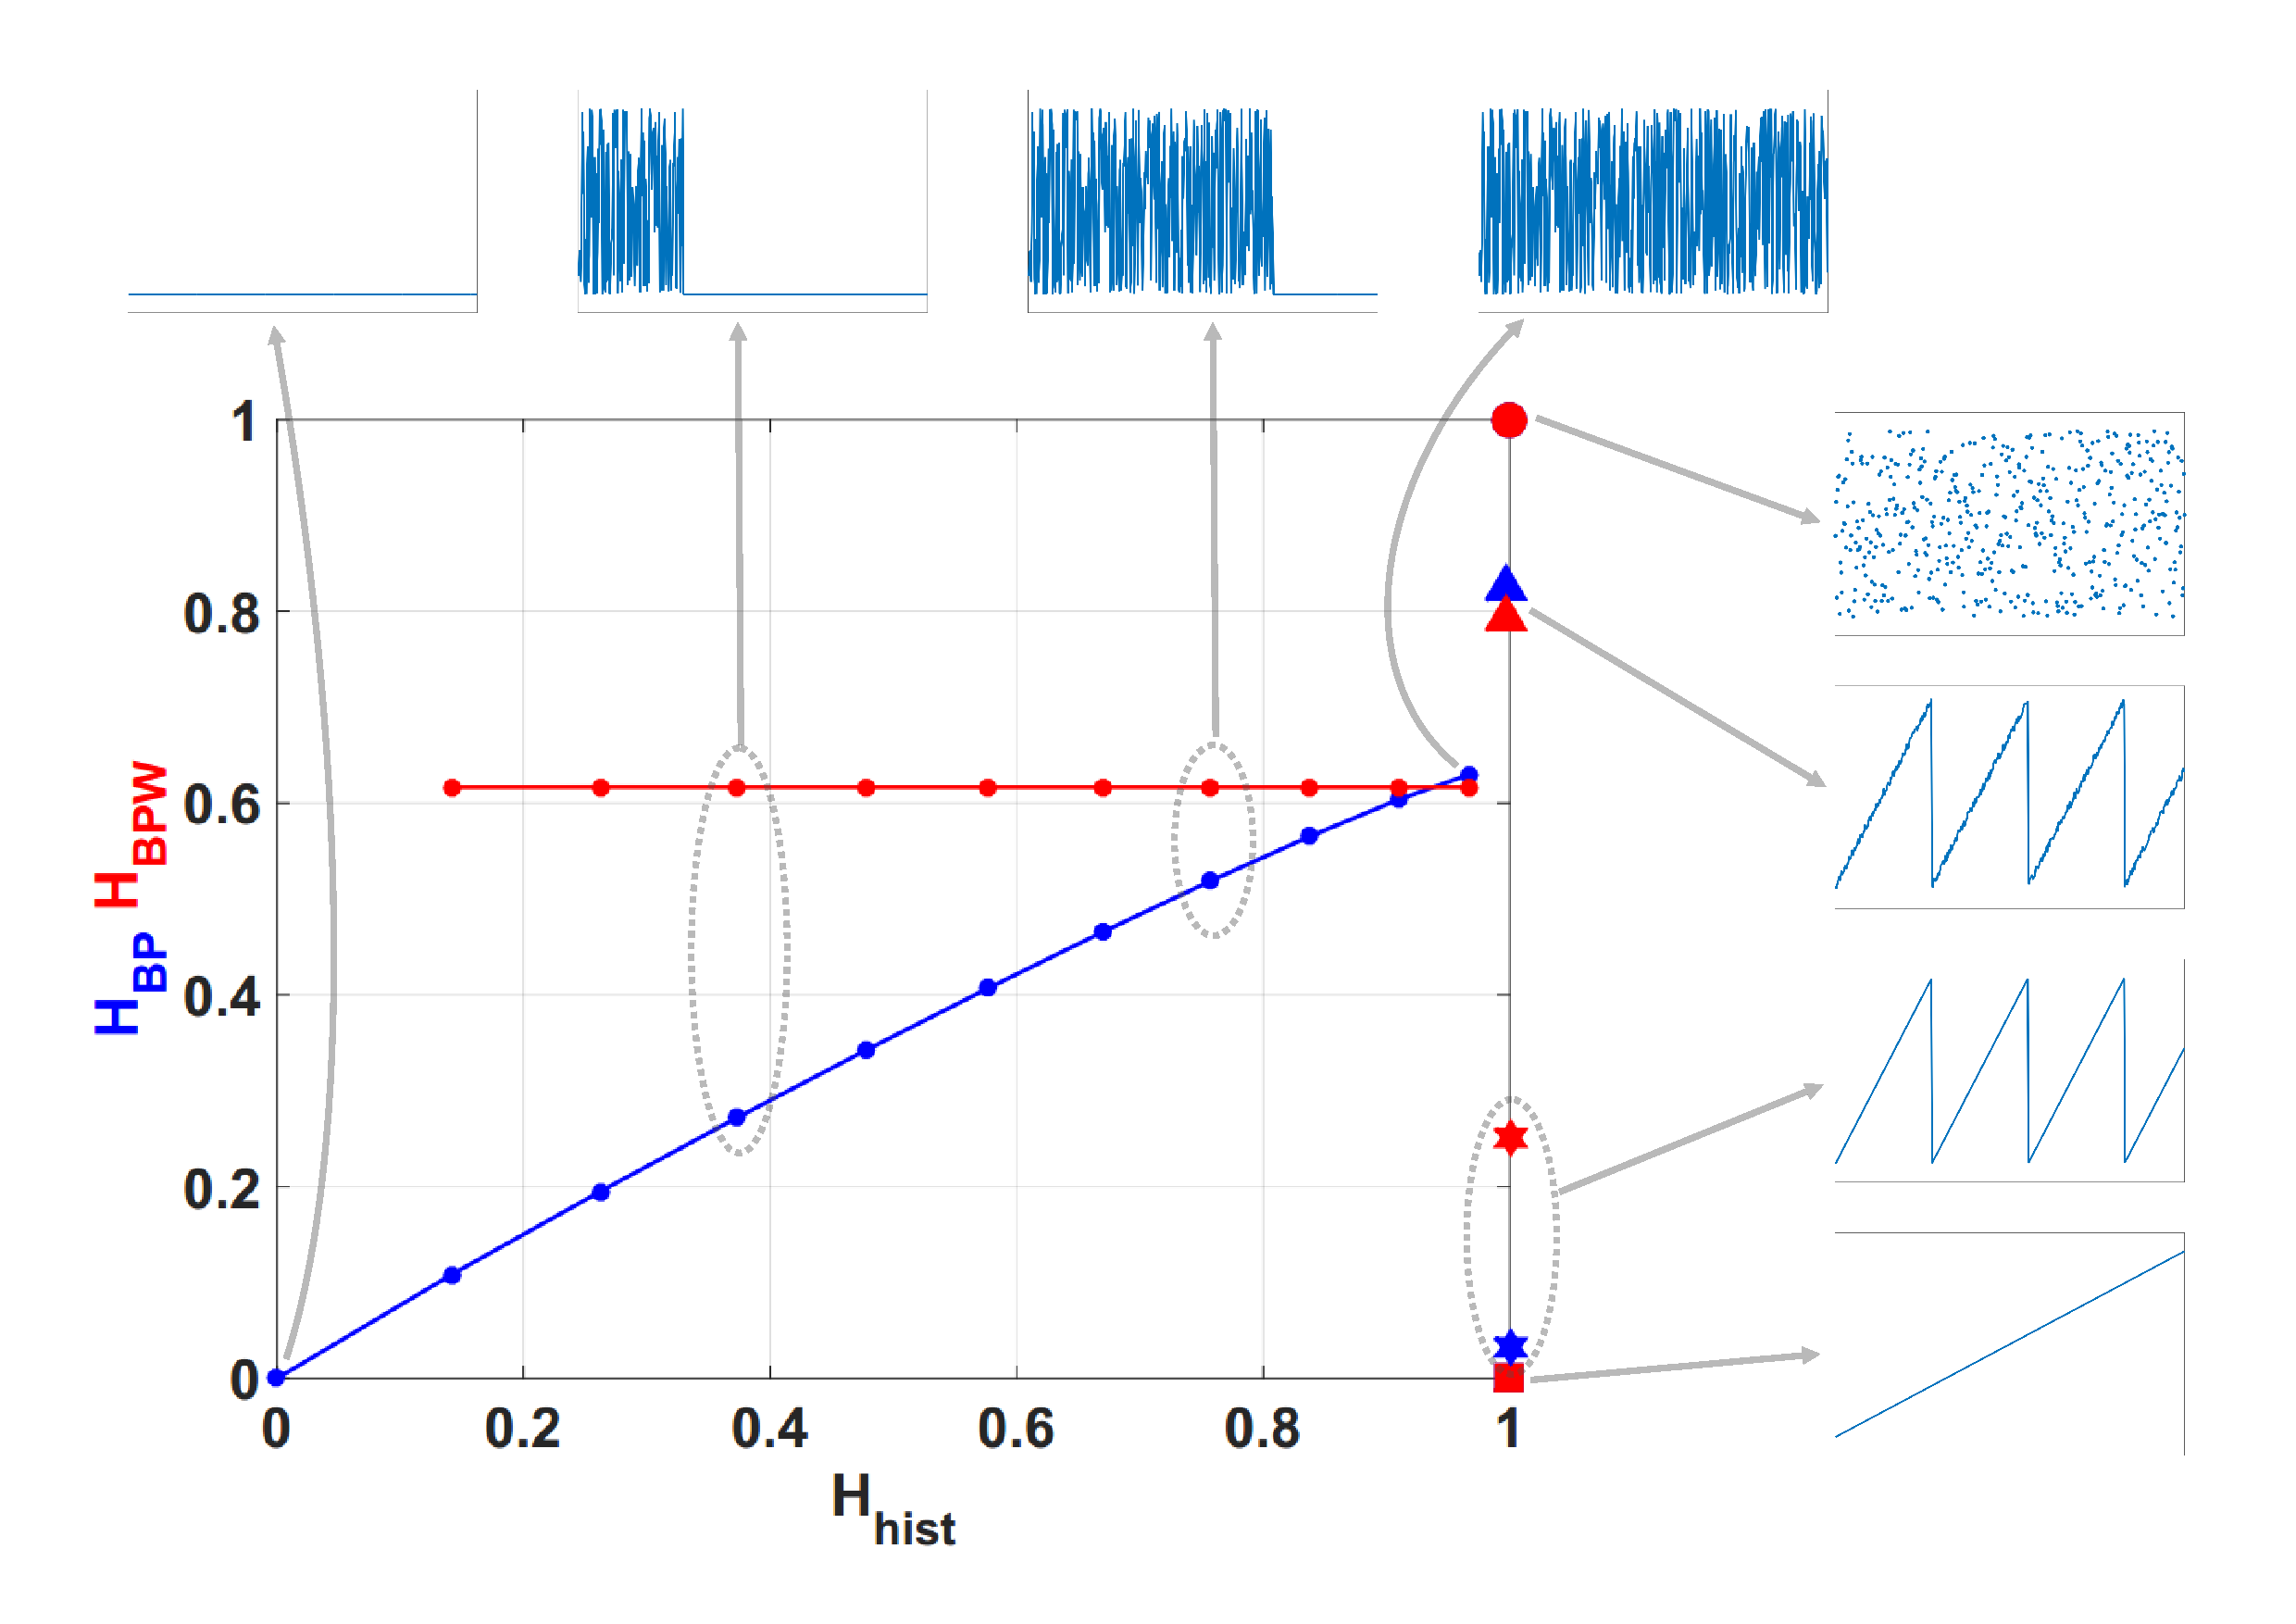
\includegraphics[width= .99\textwidth]{Fig1HHSignals}
	\caption{Causal-Non causal Entropy plane.}
	\label{fig:HH}
\end{figure}

\begin{figure}[htpb]
	\centering		
	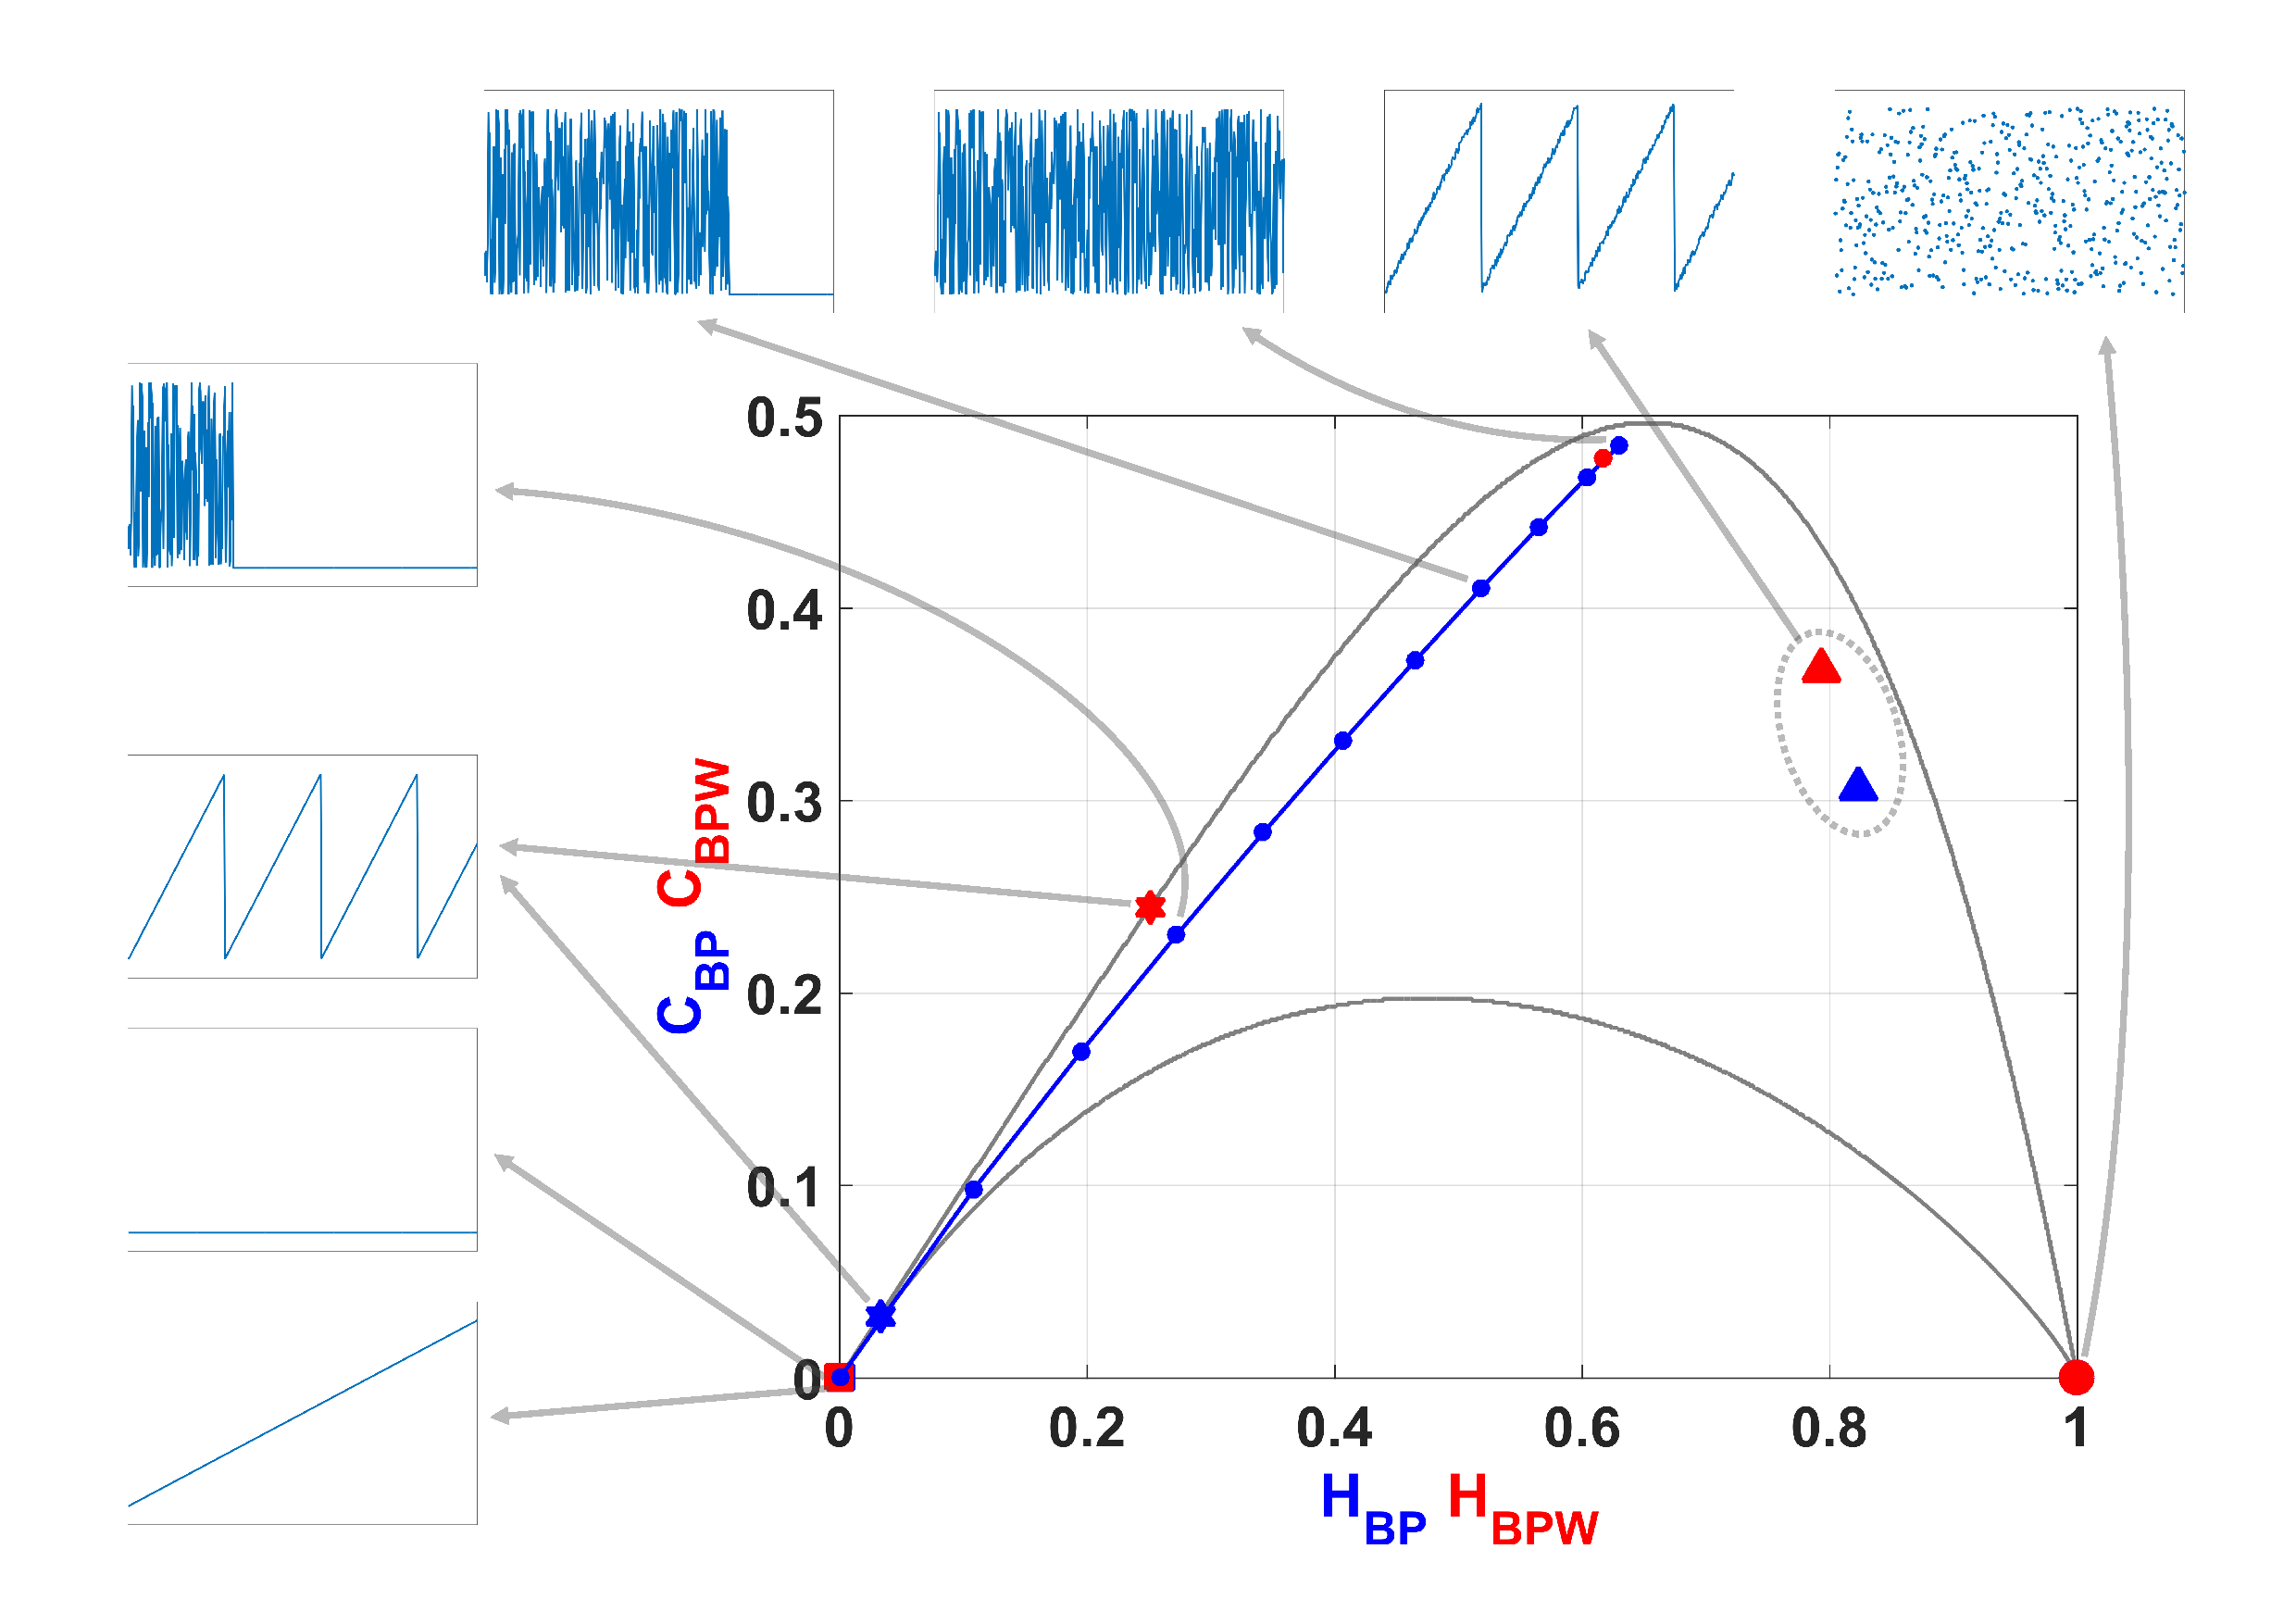
\includegraphics[width= .99\textwidth]{Fig1HCSignals}
	\caption{Causal Entropy-Complexity plane.}
	\label{fig:HC}
\end{figure}

También usamos el número de patrones perdidos MP como un cuantificador \cite {Rosso2012}.
Como mostraron recientemente Amigó y colaboradores \cite{Amigo2006,Amigo2007,Amigo2008,Amigo2010}, en el caso de mapas deterministas, no todos los patrones de orden posibles pueden materializarse efectivamente en órbitas.
De hecho, la existencia de estos patrones de orden faltantes se convierte en un hecho persistente que puede considerarse como una nueva propiedad dinámica.
Por lo tanto, para una longitud de patrón fija (dimensión de embedding $D$) el número de patrones perdidos de una serie temporal (patrones no observados) es independiente de la longitud de la serie $N$.
Obsérvese que esta independencia no caracteriza otras propiedades de la serie como la proximidad y la correlación \cite{Amigo2007,Amigo2010}.

\subsection{Entropías diferenciales}
\label{subsec:addquanti}

La entropía de Shannon $S(P)$ es el punto de partida para otros cuantificadores.

!!!!HABLAR DE LOS CONJUNTOS DE PARTICIONES Y NO SE QUE!!!

Para medir la entropía de una serie binaria es necesario 

!!!FIN DE HABLAR DE LOS CONJUNTOS DE PARTICIONES Y NO SE QUE!!!

\begin{enumerate}
	\item Entropía normalizada $H(P)$: es la entropía de Shannon dividida por su valor máximo. Por ejemplo, si usamos $S_2$ (ver arriba), se obtiene la entropía máxima para equiprobabilidad entre dos símbolos. Su valor es $S_{max}=-1/2 log(1/2)-1/2 log(1/2)=log(2)=1$; tentonces, la entropía normalizada es $H_2=S_2$. Si usamos $S_W$ la equiprobabilidad entre las $2^W$ posibles palabras (números decimales de $W$-bits) produce $S_{max}=W$ y $H_W=S_W/W$. Finalmente, para $S^{(D)}_{BP}$ la equiprobabilidad entre los $D!$ patrones de orden produce $S_{max}= log(D!)$ y $H^{(D)}_{BP}=S^D_{BP}/log(D!)$.
	\item Entropía diferencial o condicional $h$ y $h^*$ son:
	\begin{eqnarray}
	h~=~S_{W+1}-S_W\\
	h^*~=~S_{BP}^{(D+1)}-S_{BP}^{(D)}
	\end{eqnarray}
	En las expresiones de arriba $W=1,2,...$ y $D=2,3,...$, $S_0=0$ y $S_{BP}^{(1)}=0$. Esta entropía diferencial o condicional da la cantidad promedio de información requerida para predecir el símbolo $(W+1)$ (o $(D+1)$), dado los $W$ (o $D$) símbolos precedentes.
	\item Finalmente, las \emph{rate entropies} $h_0$ y $h_0^*$ \cite{Ebeling2001,Amigo2005} son dadas por:
	\begin{eqnarray}
	h_0=\lim\limits_{W\rightarrow \infty} h=\lim\limits_{W\rightarrow \infty}{S_{W}/W }\\
	h^*_0= \lim\limits_{D\rightarrow \infty} h^*=\lim\limits_{D\rightarrow \infty}{S^{(D)}_{BP}/(D-1)}
	\end{eqnarray}
\end{enumerate}

Enfatizemos algunas cuestiones importantes involucradas en los cálculos de las entropías binarias mencionadas anteriormente:
\begin{enumerate}
	\item La entropía binaria $S_2$ es no causal, mientras que ambas, la entropía de bloque $S_W$ y la entropía Bandt \& Pompe $S^{(D)}_{BP}$, son causales.
	\item La entropía de bloque $S_W$ tiene en cuenta las correlaciones entre $W$ bits consecutivos.
	La entropía Bandt \& Pompe $S^{(D)}_{BP}$ tiene en cuenta las correlaciones entre $D$ consecutivas palabras de longitud $W$.
	Ambos procedimientos de agrupación (números decimales de $W$ bits y patrones de permutación de $D$ números decimales) pueden realizarse con o sin superposición.
	La cantidad de datos requeridos para obtener buenas estadísticas es diferente dependiendo de que los procedimientos de agrupación se realicen.
	\item Para $ S_W $ solo hay un proceso de agrupación ($W$ bits agrupados para obtener una serie de números decimales $Y$).
	Definamos $\alpha$ como un parámetro de calidad estadística, dado por el cociente entre el número de elementos en la serie de tiempo simbólica $Y$ y la cantidad de símbolos en el alfabeto.
	En este documento, no aceptaremos $\alpha < 10$.
	
	Obviamente, el factor de calidad $\alpha$ aumenta con la longitud de la serie temporal:
	%
	\begin{enumerate}
		\item si el agrupamiento de $W$ bits está hecho con, dos palabras consecutivas de longitud $W$ comparten $W-2$ bits.
		En consecuencia, comenzando con un archivo con una longitud de $N$ bits obtenemos $N - W + 1$ palabras.
		Además, hay símbolos $2 ^ W$ en el alfabeto y $\alpha = (N - W + 1) / (2 ^ W)$.
		\item Si $S_W$ se evalúa sin superposición la cantidad de palabras de longitud $W$ es $floor\{N/W\}$ y el parámetro de calidad se calcula como $\alpha=floor~\{N/W\}/(2^W)$.
		Si $N \gg W$ el factor de calidad estadística es $W$ veces más bajo que el usado con superposición.
	\end{enumerate}
	
	\item En el caso de $S^{(D)}_{BP} $, hay dos procesos de agrupación involucrados.
	\begin{enumerate}
		\item Si ambos procesos de agrupamiento se realizan con superposición obtenemos $NW-D + 2$ elementos comenzando con un archivo $ N $ bits de longitud, y el factor de calidad es $\alpha = (NW-D + 2) / D!$.
		En este caso $S ^ {(D)}_{BP}$ tiene en cuenta las correlaciones entre $W + D$ bits consecutivos.
		\item Si el proceso de agrupación de $W$ bits se realiza sin superposición pero la agrupación de números decimales $D$ se realiza con superposición obtenemos $floor\{N/W\}-D+1$ elementos y el parámetro de calidad estadística es $\alpha=(floor\{N/W\}-D+1)/D!$.
		En este caso $S^{(D)}_{BP}$ incluirá correlaciones entre $WD$ bits consecutivos.
		\item Si el proceso de agrupación de $W$ bits se realiza con superposición y la agrupación de números decimales $D$ se realiza sin superposición, obtenemos $floor\{(N-W+1)/D\}$ elementos a partir de un archivo de $N$ bits.
		El factor de calidad estadística es $\alpha=floor\{(N-W+1)/D\}/D!$ y $S^{(D)}_{BP}$ tiene en cuenta correlaciones de $W+D-1$ bits.
		\item Si ambos procesos de agrupación se realizan sin superposición, obtenemos $floor\{floor\{N/W\}/D\}$ elementos a partir de un archivo de longitud de  $N$ bits.
		El factor de calidad estadística es $\alpha=floor\{floor\{N/W\}/D\}/D!$ y $S^{(D)}_{BP}$ tiene en cuenta las correlaciones entre $WD$ bits consecutivos.
	\end{enumerate}
\end{enumerate} 
\subsection{Cuantificador de Entropías Implementado en FPGA}
\label{ssecCuantiImpFPGA}

En esta Sección se describe la implementación de un sistema de medición de entropías.
El diseño fue optimizado para ser implementado en un microcontrolador simple y pequeño, conservando una precisión aceptable.
El sistema permite medir entropías a señales generadas internamente por código y a señales externas analógicas muestreadas.
Se utilizó la placa de desarrollo \textit{M1AFS-embedded kit} de ACTEL.
En la FPGA (\textit{Field Programmable Gate Array}) se instanció un microcontrolador 8051 al que se programó en lenguaje C.
Se detalla el diseño del \textit{hardware} y \textit{software} y los resultados obtenidos.
Al momento hay muy poca bibliograf\'ia sobre implementaciones en \textit{hardware} de estos cuantificadores \cite{DeMicco2013}.

La entropía es empleada en diversas aplicaciones, como por ejemplo, en la detección de anomalías en flujos de datos IP \cite{Gu2005,Wagner2006, actelM1AFS1500}.
En \cite{Subramanya2008} se presentó un diseño y simulación en FPGA de un cuantificador de entropía, sin embargo, actualmente no hay disponibles implementaciones en \textit{hardware} de este cuantificador.

En esta tesis se implementó un sistema que calcula la entropía para la PDF asociada a una serie de datos.
Se analizan PDFs causales y no causales.
Los datos pueden tener un origen digital (generados mediante códigos), o bien provenir del muestreo de señales analógicas.
Se utilizó la placa de desarrollo \textit{M1AFS-embedded kit}, basado en el chip \textit{M1AFS1500} que se destaca por tener un bloque analógico embebido en el mismo encapsulado de la FPGA.
Luego, se verificó la exactitud numérica del cuantificador implementado comparando sus resultados con un programa patrón.
A partir del máximo error detectado se determinó la exactitud numérica del sistema.

\subsubsection{\textit{Hardware} Implementado}
\label{sec:Hardware}

El diseño del \textit{hardware} se basó en el que provee ACTEL en \cite{Core8051sH}, basado en el microcontrolador 8051, interfaces y periféricos.
Fue realizado con el paquete de programas \textit{Libero~Soc~v11.3\textsuperscript\copyright} de ACTEL.
Se utilizó la placa de desarrollo \textit{M1AFS-EMBEDDED-KIT} que contiene una FPGA \textit{M1AFS1500} de ACTEL y periféricos \cite{actelM1AFS1500}.
El chip \textit{M1AFS1500} contiene embebido un bloque analógico que consiste en nueve adaptadores direccionables de cuatro entradas cada uno, un multiplexor analógico de 32 entradas y un conversor analógico-digital configurable.

El sistema implementado puede dividirse en tres etapas principales como se muestra en la Figura \ref{Fig:Sistema}: una primera etapa de Adquisición de datos, que convierte a palabras digitales las señales del mundo analógico, una Lógica de Cálculo, que se vale de la memoria SRAM para llevar a cabo los cálculos y coordinar las interfaces y una etapa de Presentación de resultados, que envía los resultados de la medición a una computadora a través de la interfaz \textit{USB-to-UART}.
%
\begin{figure}
	\centering
	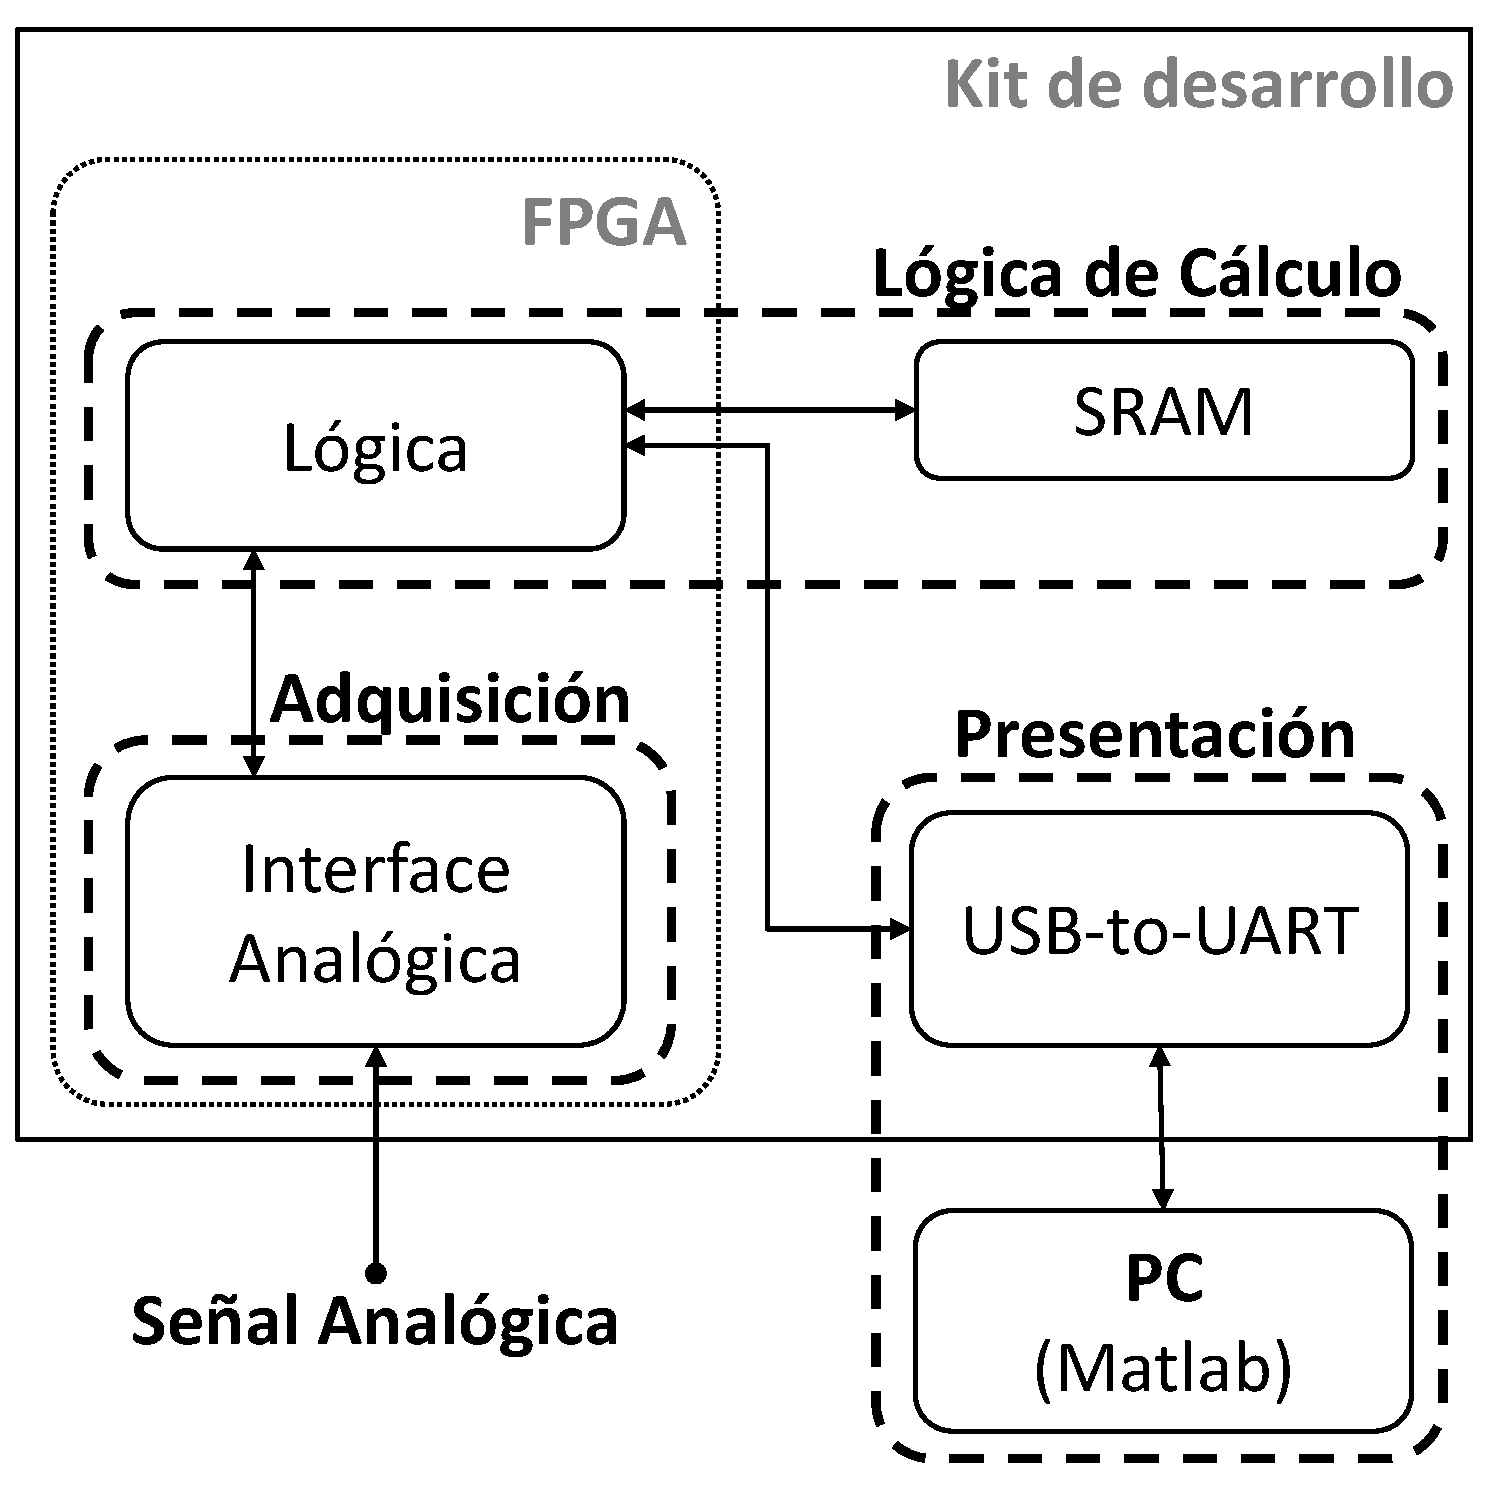
\includegraphics[width=.8\columnwidth]{Sistema.pdf}\\
	\caption{Esquema del sistema completo.}\label{Fig:Sistema}
\end{figure}

\begin{enumerate}
	\item \textit{Etapa de Adquisición:}
	
	Para ingresar los datos analógicos a ser evaluados utilizamos la entrada de tensión $AV2$ del \textit{Analog~Quad~2} del bloque analógico.
	Se encuentra direccionada en el canal siete del multiplexor analógico y fue configurada para un rango de tensiones de entrada de 0~V a 4~V.
	El conversor analógico-digital se configuró con una resolución de 12~bits.
	En este primer prototipo la frecuencia de muestreo máxima alcanzada fue de 16~ks/s limitada por el retardo necesario en el procesamiento de la lógica.
	
	\item \textit{Lógica de cálculo:}
	
	En esta etapa se realizan los cálculos y la sincronización entre periféricos.
	En la Figura \ref{fig:logica} pueden verse los bloques principales que la componen.
	%
	\begin{figure}
		\centering
		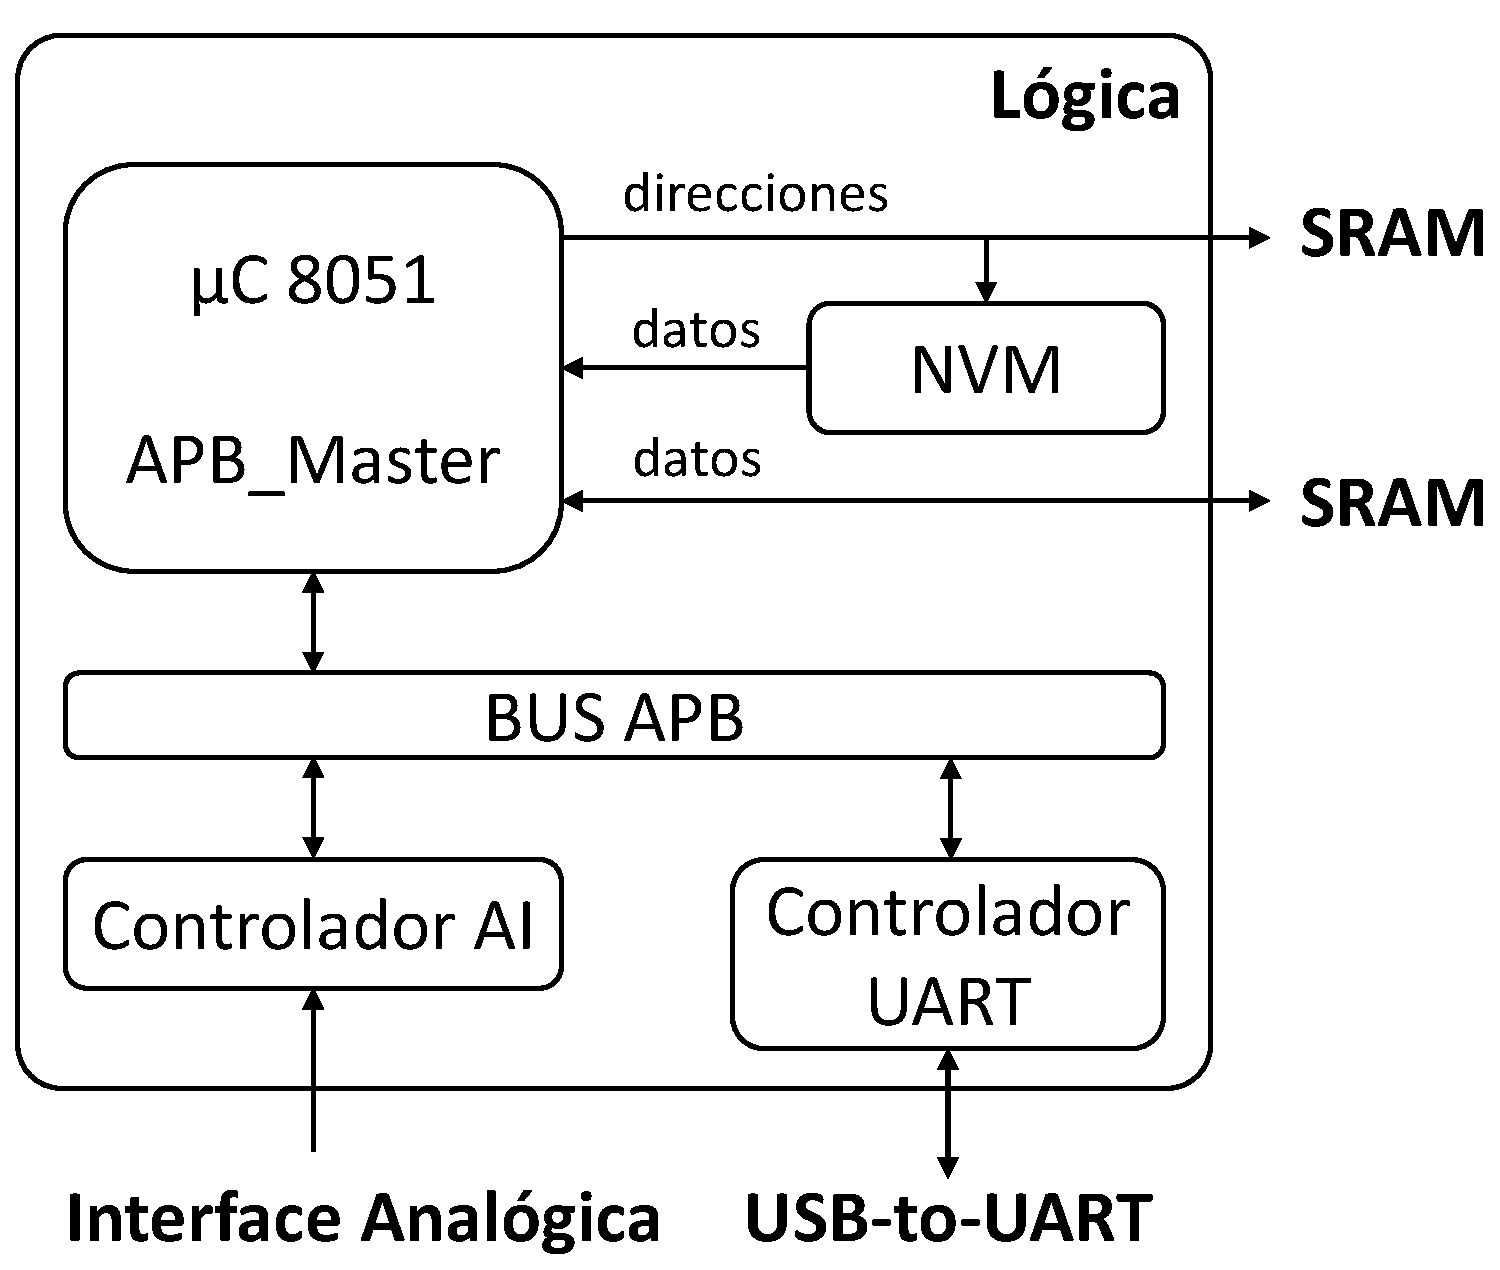
\includegraphics[width=.75\columnwidth]{Logica.pdf}\\
		\caption{Detalle de la lógica de cálculo.}\label{fig:logica}
	\end{figure}
	
	El núcleo de la implementación es un \textit{Core} 8051 que provee ACTEL en su catálogo de librerías.
	Se trata de un microcontrolador que contiene la lógica principal del microprocesador 8051 de Intel, sin sus periféricos.
	Este micro tiene una arquitectura Von Newman con un bus de direcciones de 16~bits, lo que limita nuestro diseño a $64~KB$ de memoria de código y $64~KB$ de memoria de datos.
	
	Sobre este microcontrolador corre el programa que realiza los cálculos presentados en la Sección \ref{sec:ITQs}.
	Se encarga de, a partir de los datos de entrada, obtener las PDFs ($BP$ e $hist$) y de realizar los cálculos para la obtención de las entropías, según la Ecuación \ref{shannon-disc-normalizada}.
	El \textit{software} implementado se describe más detalladamente en la Sección \ref{sec:Software}.
	
	La memoria de código es una memoria no volátil (NVM) implementada con los bloques flash internos de la FPGA.
	Ocupa las direcciones desde 0x0000 hasta 0xFFFF y se escribe con el contenido de un archivo en formato hexadecimal durante la compilación.
	
	Las funcionalidades del sistema son ampliadas mediante la conexión de periféricos a través de la interfaz APB.
	
	Para realizar la comunicación con la PC utilizamos el \textit{Controlador UART}.
	La salida de este bloque es dirigida hacia afuera de la FPGA y se conecta a un chip \textit{USB-to-UART} que se encuentra soldado a la placa del kit de desarrollo.
	
	El bloque analógico es controlado por el \textit{Controlador AI}, que direcciona y sincroniza sus entradas.
	
	\item \textit{Presentación:}
	
	La etapa de Presentación de los datos involucra al chip adaptador \textit{USB-to-UART} que se encuentra en la placa de desarrollo y es manejado tanto por el programa que corre en la FPGA como por el \textit{software} que corre sobre la PC.
	El chip adaptador \textit{USB-to-UART} es el responsable de adaptar la entrada-salida UART de la lógica a una entrada-salida USB estándar mediante la cual es posible interactuar con la PC.
	Por otra parte el programa que corre en la PC se encarga de la interfaz con el usuario y es descripto en detalle en la siguiente Sección.
	
\end{enumerate}

\subsubsection{\textit{Software} Implementado}
\label{sec:Software}

El funcionamiento del sistema se logra mediante la interacción de dos programas.
Uno corriendo en la PC y otro en el microcontrolador implementado en la FPGA.
Puede verse un diagrama de flujo de ambos programas y la interacción entre ellos en la Figura
\begin{figure}[htpb]
	\centering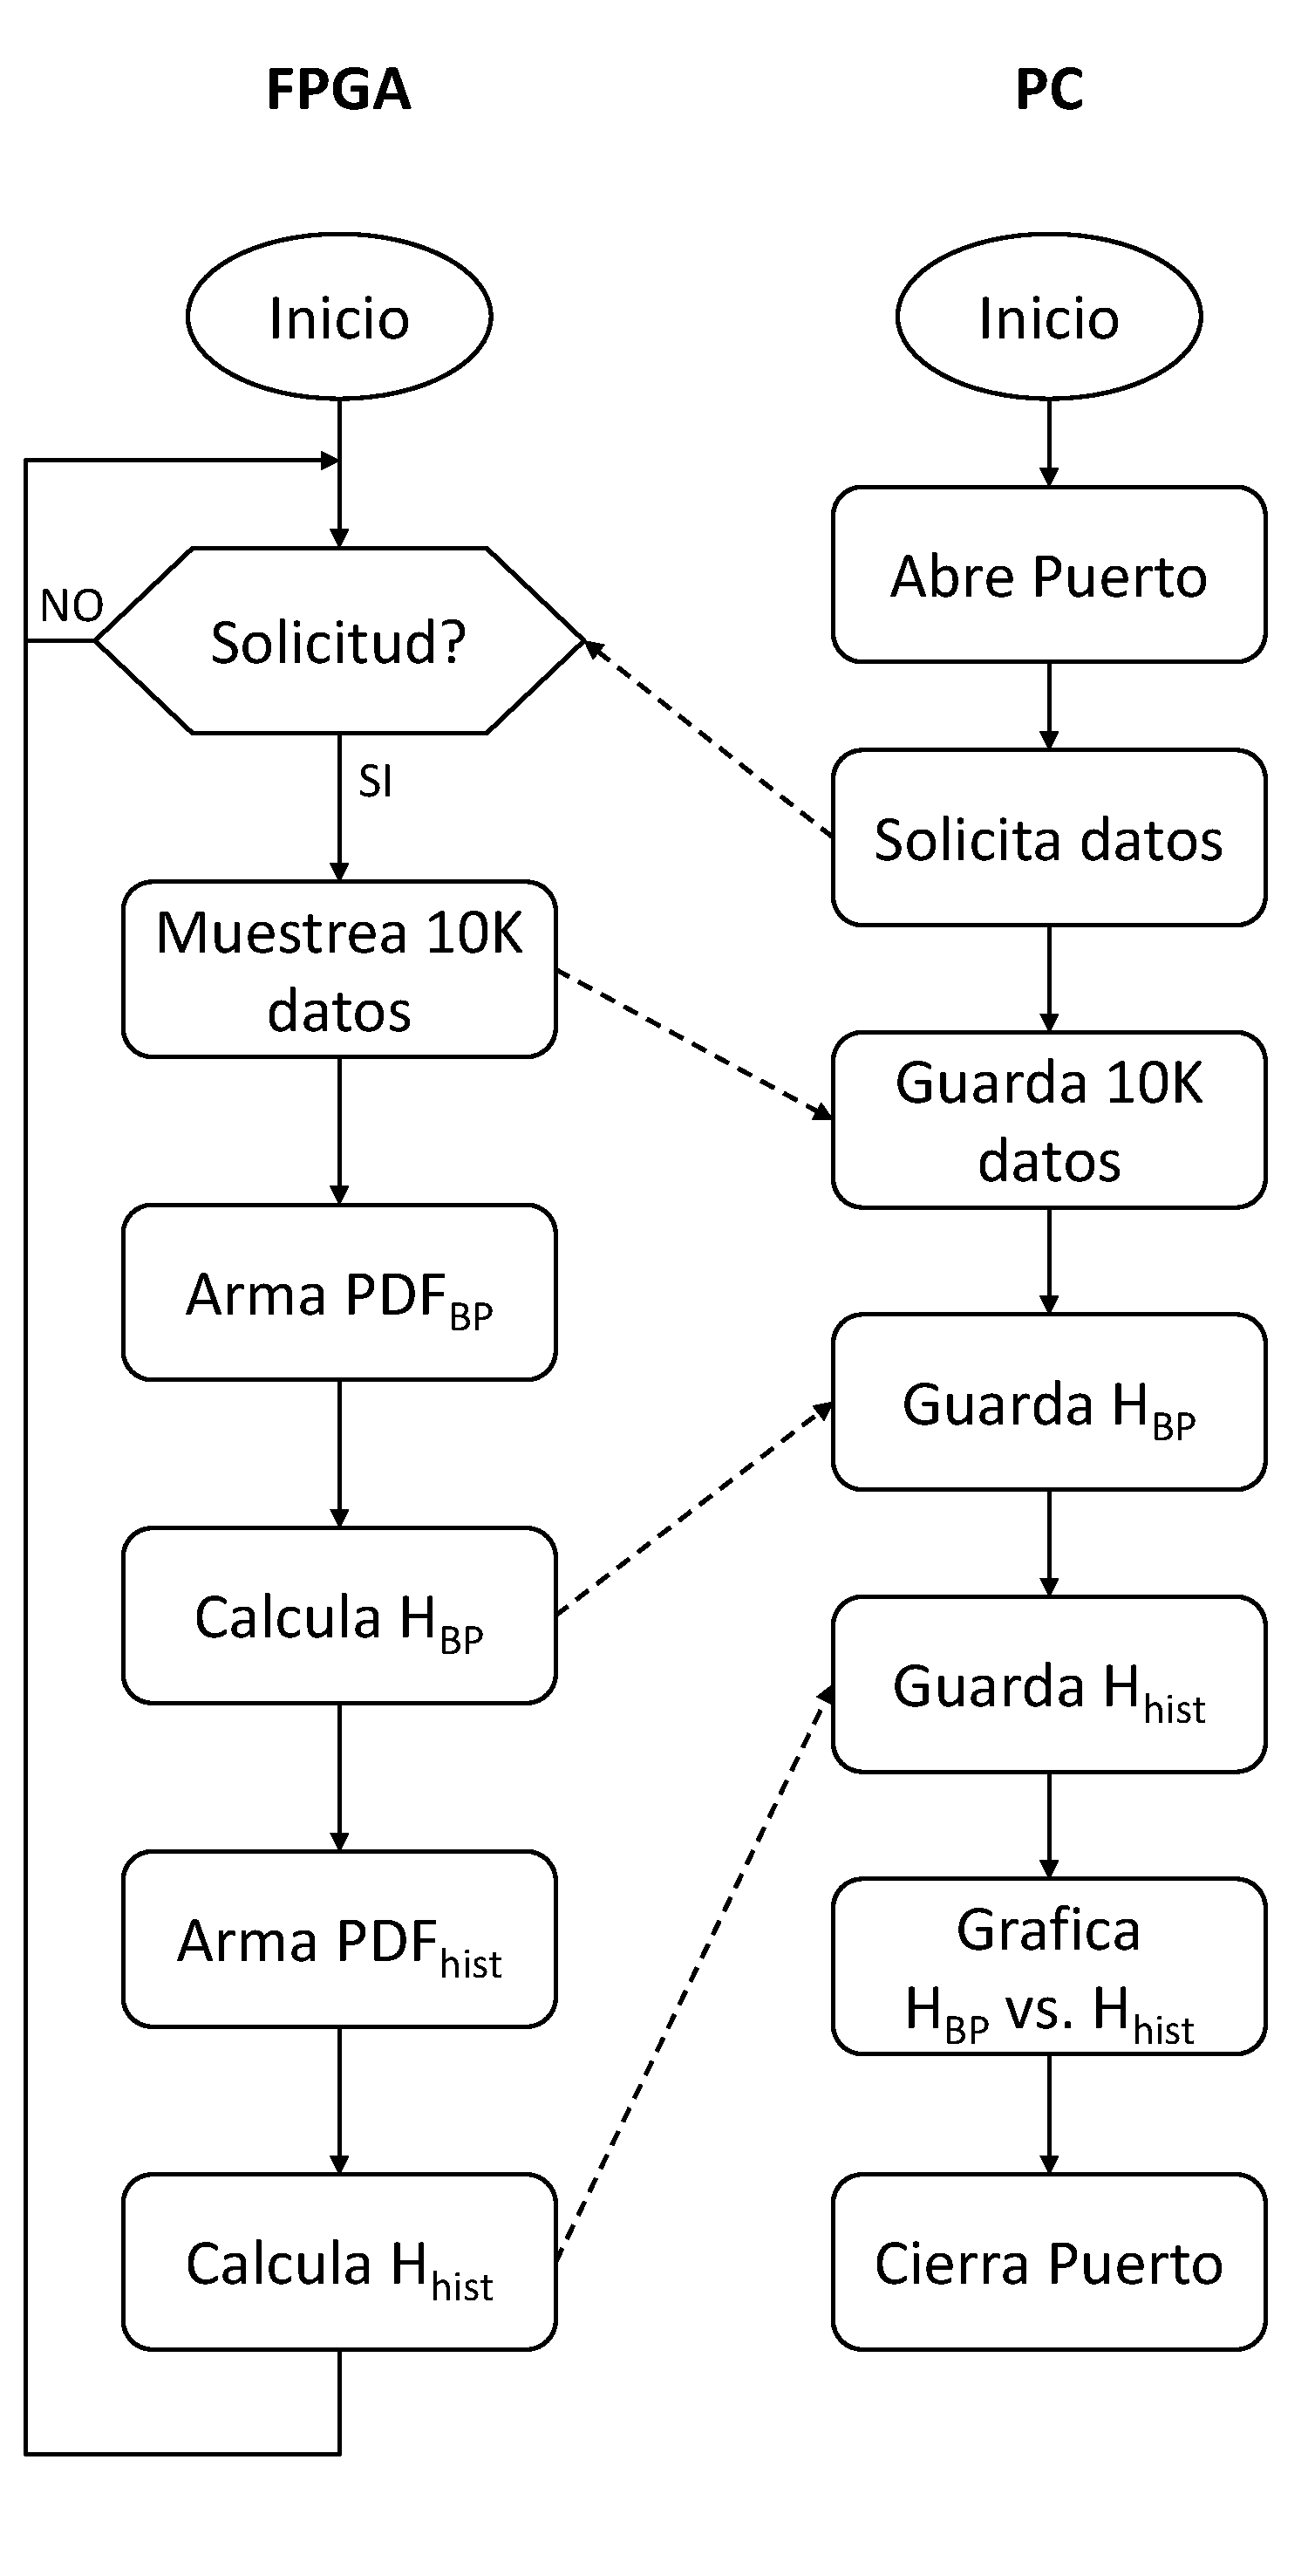
\includegraphics[width=0.7\columnwidth]{Soft}
	\caption{Diagrama de flujo del \textit{software} implementado.}\label{fig.softflow}
\end{figure}

En la PC corre un \textit{script} de Matlab que se encarga de abrir el puerto serie en donde se encuentra mapeado el USB, solicitar los datos, tomar los resultados del mismo puerto, graficarlos en un plano $H_{BP}$ vs. $H_{hist}$ y cerrar el puerto.

Sobre el microcontrolador en la FPGA corre un programa escrito en lenguaje C y compilado para el microcontrolador 8051 utilizando la herramienta \textit{SoftConsole~IDE~v3.4\textsuperscript\copyright}.
El firmware es una modificación del usado en \cite{Core8051sS}. Cuando se presenta una solicitud de datos por el puerto UART, se guardan los datos muestreados de la entrada analógica.
Luego, se recorre este vector generando las $PDF_{hist}$ y $PDF_{BP}$, a las que se les calcula sus respectivas entropías $H_{hist}$ y $H_{BP}$.
Estos resultados son enviados a la PC mediante el mismo puerto.

Con el fin de validar el sistema, el programa en la FPGA envía a  Matlab el vector de datos muestreados, para que se puedan calcular en la PC sus entropías y compararlas con los resultados del sistema implementado.

\subsubsection{Resultados}
\label{sec:resultados}

Como se dijo, para testear el sistema se compararon los resultados obtenidos por el sistema implementado y por un programa patrón que corre en la PC.
Para esto, se generaron $10~000$ muestras de señales con distintas formas de onda tanto externas (analógicas) como internas (digitales).

Las señales digitales fueron generadas por código en el microcontrolador, una corresponde a la función rand() de C y la otra al mapa caótico Logístico con parámetro r=4.

Las señales analógicas fueron generadas con el generador de funciones \textit{HP33120A}.
Tienen una amplitud de $4~Vpp$ y un nivel de continua de $2~V$ de forma de aprovechar todo el rango del conversor analógico-digital y aumentar la relación señal-ruido.
En los cuatro casos la frecuencia de las señales fue de $100~Hz$ y la velocidad de muestreo de $16~ks/s$.

El cuadro \ref{tablaErrores} muestra el error absoluto entre los resultados de los cuantificadores calculados en la FPGA comparados con los resultados calculados con el programa patrón sobre los mismos datos.
%
\begin{table}
	\centering
	\begin{tabular}{@{\extracolsep{\fill}}| c| c | c |c |}
		\hline
		\textbf{{Generador}} & \textbf{{Origen}} & \textbf{{Error}} \textbf{{$H_{BP}$}} & \textbf{\textbf{{Error}}} \textbf{{$H_{hist}$}} \\ \hline
		{Rand}               & {Digital}         & {$1,7421E^{-6}$}                     & {$2,6977E^{-6}$}                                \\ \hline
		{Logístico}          & {Digital}         & {$0,4256E^{-6}$}                     & {$94,693E^{-6}$}                                \\ \hline
		{Triangular}         & {Analógico}       & {$6,3445E^{-6}$}                     & {$2,0028EE^{-6}$}                               \\ \hline
		{Senoidal}           & {Analógico}       & {$6,3151E^{-6}$}                     & {$5,6506E^{-6}$}                                \\ \hline
		{Cuadrada}           & {Analógico}       & {$0,1797E^{-6}$}                     & {$1,9930EE^{-6}$}                               \\ \hline
		{Rampa}              & {Analógico}       & {$245,00E^{-6}$}                     & {$1,0876E^{-6}$}                                \\ \hline
	\end{tabular}
	\caption{Error de los cuantificadores evaluados en la FPGA con respecto a los resultados calculados por el programa patrón.}\label{tablaErrores}
\end{table}

La Figura \ref{fig:resultados} muestra los valores entregados por la FPGA en el plano $H_{BP}$ vs. $H_{hist}$.
%
\begin{figure}[htb]
	\centering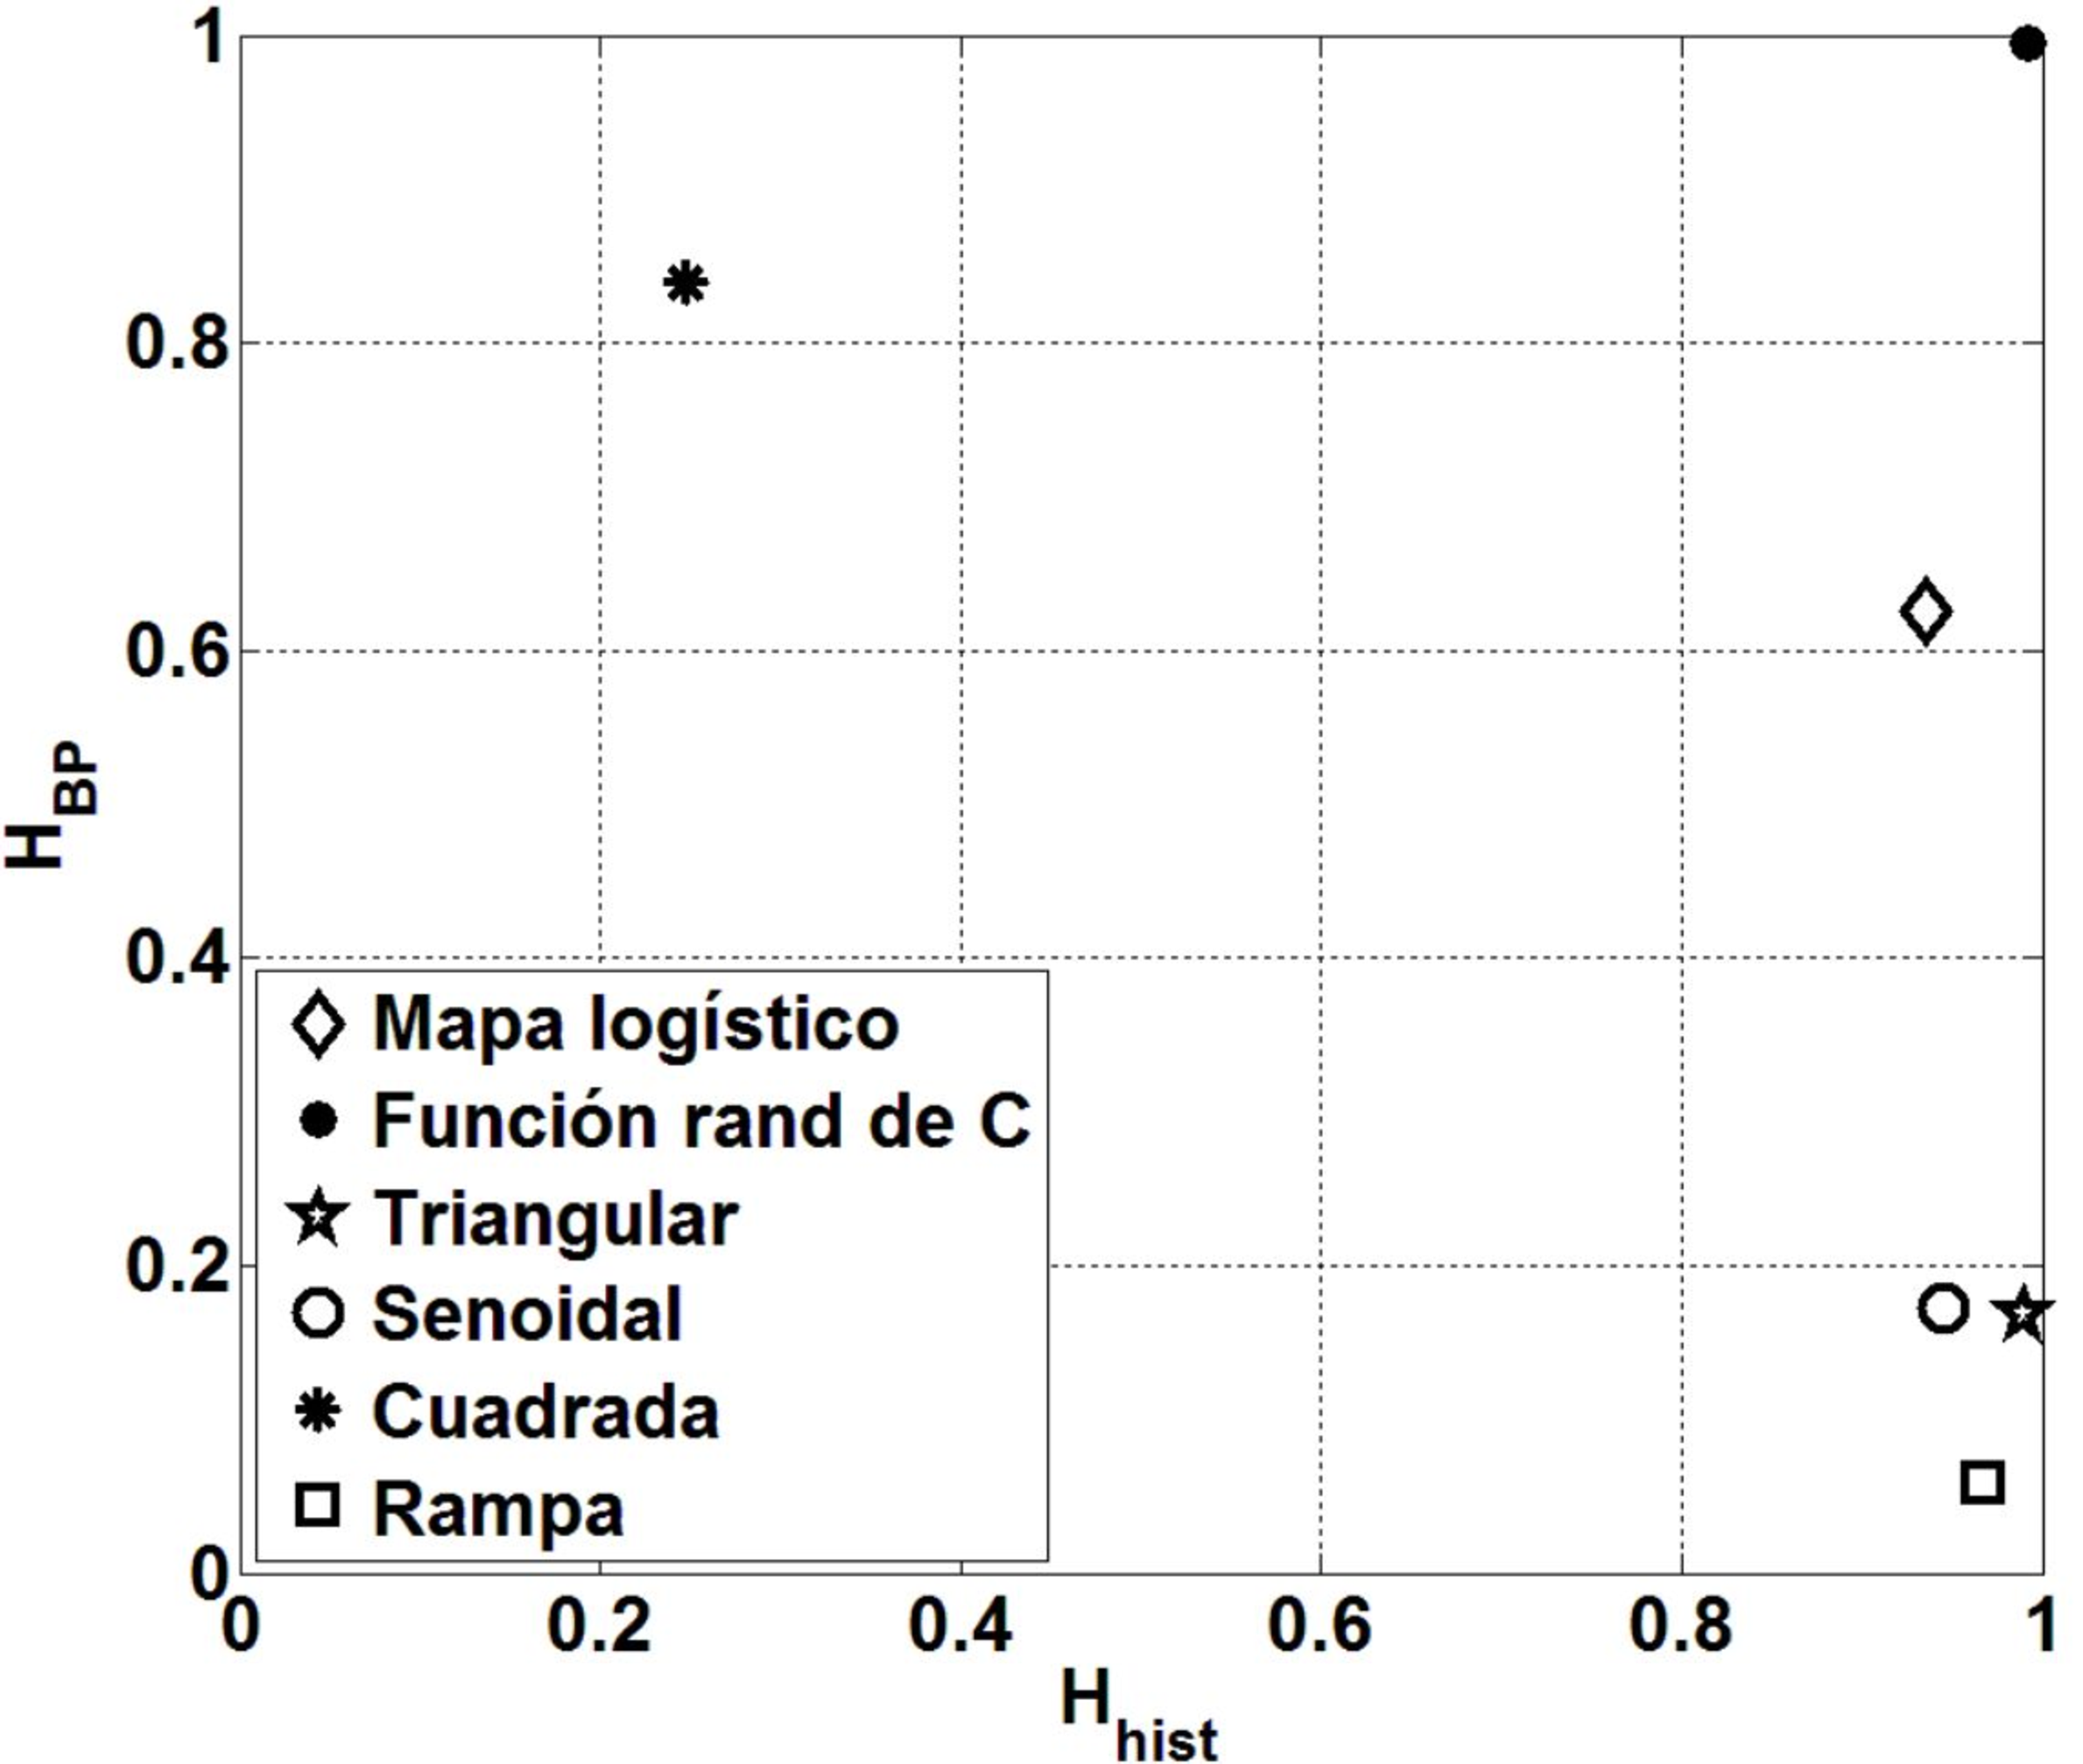
\includegraphics[width=.75\textwidth]{resultados}
	\caption{Resultados de las mediciones.}\label{fig:resultados}
\end{figure}

Los resultados de la compilación nos permiten conocer los recursos de la FPGA utilizados por el sistema completo y la cantidad de memoria ocupada por el \textit{software} que corre en el microcontrolador.
Recordemos que esta es una implementación de \textit{hardware} rígida, es decir primero se arma el circuito en la FPGA (microcontrolador, periféricos, etc.) y luego se carga el \textit{software} sobre él.

El reporte de la compilación de \textit{hardware} devuelto por el \textit{Place and Route} se muestra en la Figura \ref{fig:hard}. Podemos ver que la implementación utiliza un 19\% de los recursos lógicos de la FPGA, el $21\%$ de las celdas de entrada-salida y el $28\%$ de los bloques de memoria.
%
\begin{figure}[htb]
	\centering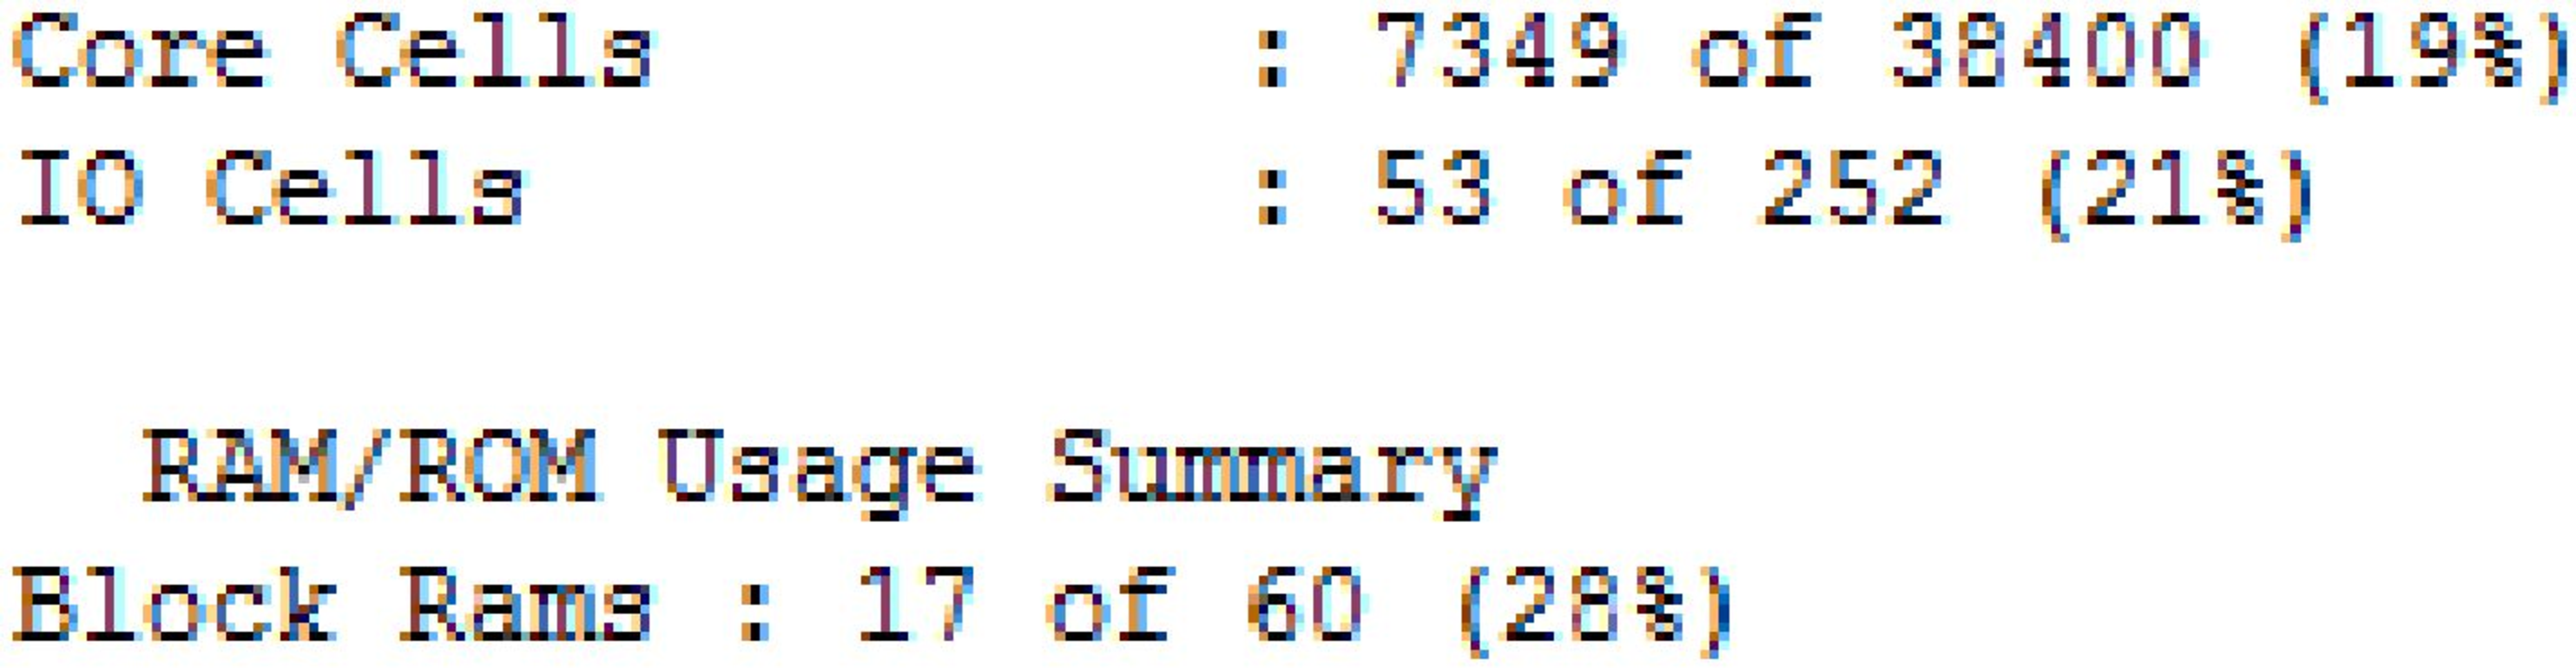
\includegraphics[scale=.13]{reporteHard}
	\caption{Recursos empleados por el \textit{hardware} del sistema.}\label{fig:hard}
\end{figure}

El reporte de la compilación de \textit{software} se muestra en la Figura \ref{fig:soft}.
Podemos ver que la memoria FLASH no volátil se encuentra ocupada al $15,4\%$.
Por otro lado, de las $47~145$ direcciones de memoria SRAM ocupada, $4~096$ son ocupadas por el bus APB y $43~049$ por las variables del programa.
%
\begin{figure}[htb]
	\centering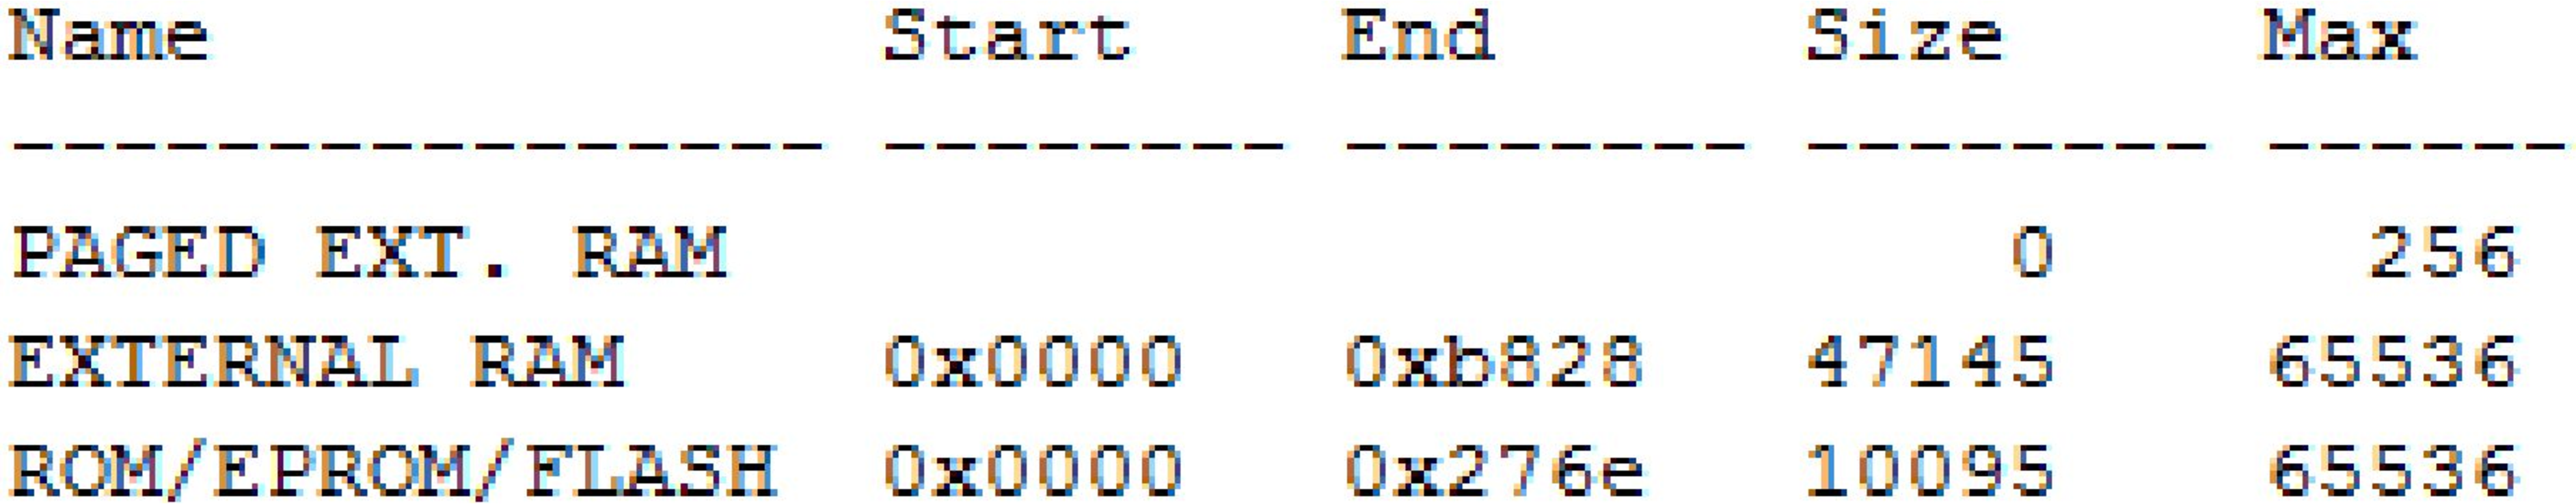
\includegraphics[scale=.13]{reporteSoft}
	\caption{Recursos empleados por el \textit{software} del sistema.}\label{fig:soft}
\end{figure}

El programa debió ser adaptado al microcontrolador instanciado en la FPGA.
Estas modificaciones hacen que la salida del sistema implementado no sea igual a la de un programa que corre en la PC, al cual tomamos como programa patrón.
Por esto se testeó el error cometido, para tener una cota y determinar si los resultados de los cuantificadores son correctos.
El programa patrón utiliza aritmética de $64~bits$ en punto flotante norma IEEE754-64~bits y emplea la librería math.h \cite{Mathe}.
Para el algoritmo en la FPGA se disminuyó la aritmética a 32 bits de punto flotante norma IEEE754-32~bits.
También se requirió el cálculo de la función logaritmo, que se implementó mediante un algoritmo de CORDIC.
En el Cuadro \ref{tablaErrores} se ve que el error absoluto no supera el sexto decimal, esto indica que se detecta diferencia recién a partir del quinto dígito decimal.

En la Figura \ref{fig:resultados} puede verse como los cuantificadores $H_{BP}$y $H_{hist}$ diferencian claramente las propiedades estadísticas de las series de datos analizadas.
Las señales Senoidal, Rampa y Triangular presentan un valor alto de $H_{hist}$ porque tienen casi todos los valores que es capaz de generar el conversor Analógico-Digital.
Sin embargo, la mezcla de estos datos es mala por tratarse de señales periódicas totalmente predecibles, esto se ve en el bajo valor de $H_{BP}$.
Un caso interesante de analizar es la señal Cuadrada.
El efecto del ruido aditivo es especialmente notable en las zonas en donde el valor de la señal debería ser constante.
Se generan dos Gaussianas muy finas en torno a los valores ideales en la $PDF_{hist}$, esto no afecta demasiado el valor calculado $H_{hist}$, sin embargo, para la $PDF_{BP}$, se calcula el patrón de orden directamente a la señal ruidosa, por lo que el valor de $H_{BP}$ es más alto que el esperado.
La señal generada mediante la función rand de C, presenta las mejores propiedades estadísticas ubicándose en el punto $\sim(1,1)$.
\subsection{Dinámica de los ITQ's con AWGN y Banda Limitada}
\label{ssec:TDdS}
	
En esta Sección exploramos la respuesta de un sistema de medición de entropías en presencia de ruido aditivo y señales filtradas.
Esta inquietud surge como resultado de la implementación detallada en la Sección \ref{ssecCuantiImpFPGA}.
El filtrado es inherente al ancho de banda del sistema de medición y las señales a medir siempre están contaminadas con ruido, por lo tanto es necesario caracterizar la respuesta de nuestro sistema de medición ante estos dos procesos.
Este trabajo es complementario al desarrollo de un sistema de medición de entropías implementado en FPGA.

\subsubsection{Filtrado digital}
\label{sec:filtrado}

Ya sea en la elección de un filtro como en cualquier problema de diseño en ingeniería, generalmente no es posible dar una respuesta posible acerca de cuál es al mejor solución. Se discute la posibilidad de la implementación de distintos filtros porque no hay un solo método de diseño ni un sólo tipo de filtro mejor para todas las circunstancias. La elección del tipo de filtro depende de la importancia de sus ventajas aplicadas a cada problema.

Un filtro ideal es aquel en el que la respuesta en frecuencia es unitaria en el rango de las frecuencias de paso, cero en la banda de rechazo y no posee banda de transición. Dada la inherente periodicidad de la respuesta en frecuencia para tiempo discreto esta tiene la apariencia de un tren rectangular en el dominio de las frecuencias, sin embargo en este trabajo sólo se muestra la frecuencia normalizada en el intervalo $(0,1)$. Entonces la transferencia de un filtro pasabajos ideal en frecuencia normalizada quedaría:
\begin{equation}
H_{LP}=
\left\{ 
\begin{aligned}
&1,\qquad|f-0,5|>f_c\\
&0,\qquad|f-0,5|<f_c
\end{aligned}
\right.
\end{equation}
Ecuación definida en el intervalo de frecuencias normalizadas $f\in\left(0,1\right)$.

El hecho de que no podemos contar con series de valores infinitamente largas para ser filtradas, equivale a decir que disponemos de una serie de muestras enventanada.
Como el producto en el dominio del tiempo equivale a una convolución en el dominio de la frecuencia, podemos estudiar el efecto que este enventanado tiene sobre la respuesta frecuencial del filtro.
Consideremos la ventana más sencilla; la ventana rectangular. Supongamos que la aplicamos sobre una versión retardada de la respuesta ideal, su efecto en el dominio de la frecuencia será la convolución entre la respuesta de nuestro filtro ideal y la transformada esta ventana rectangular, es decir una función $sinc$ de período $1/N$ en donde $N$ es la cantidad de muestras que entran en la ventana.

El efecto de enventanado o truncaminto de la respuesta es doble: por una parte, la anchura del lóbulo principal está relacionada con la aparición de una banda de transición en el filtro. Por otra, la presencia de lóbulos laterales (secundarios) lleva a la aparición de un ripple u oscilaciones en la respuesta en frecuencia, en ambas bandas, (más apreciable en la banda no pasante).
La aparición de los lóbulos secundarios se debe a que la ventana rectangular presenta una discontinuidad abrupta que, al pasar al dominio de la frecuencia, conlleva un reparto de la energía sobre todo el espectro a causa del aliasing.

Una opción que se plantea es generalizar el concepto de ventana y emplear ventanas más suaves que la rectangular para realizar el truncamiento de la respuesta deseada, esta técnica es una de las formas de realizar un filtro FIR.
Sin embargo, si analizamos la transformada de la ventana cuadrada vemos que presenta valores nulos cada $1/N$, que son los mismos lugares en donde aparecen las componentes espectrales de la DFT. Esto significa que los efectos de la ventana rectangular aparecen al convertir la respuesta de este filtro a tiempo continuo.

Otra opción sería diseñar un filtro analógico y transformar su respuesta a frecuencia discreta. Para esto existen fórmulas cerradas de diseño, por lo que es posible satisfacer casi cualquier especificación preestablecida. La utilización de esta técnica da como resultado un filtro IIR. Comparado con un filtro FIR, un filtro IIR requiere un orden mucho menor para cumplir las especificaciones de diseño.

En este caso se analizó la respuesta del sistema en el dominio digital.
Además, es necesario filtrar las componentes espectrales de a una, lo que requiere una banda de transición muy estrecha, esto reduce el conjunto de filtros posibles.
Por el lado del IIR se probó un filtro elíptico, este filtro presenta una banda de transición muy estrecha a costa de un ripple que aparece tanto en la banda de paso como en la de rechazo.
Por el lado del filtro FIR se utilizó un filtro ideal con una ventana rectangular que abarca toda la serie de valores.

\subsubsection{Resultados}

Para representar la dinámica en función del filtrado, se eligieron dos señales representativas (cuadrada y senoidal) y se les calcularon los cuantificadores descriptos en la Sección \ref{sec:ITQs} luego de ser filtrados por los filtros elegidos en la Sección anterior. Por otro lado, se calcularon los mismos cuantificadores a una señal de ruido blanco gaussiano.

En la Figura \ref{fig:flowchart} se muestra el procedimiento utilizado. Primero se generó un vector de ruido blanco gaussiano de $N=50~000$ muestras, la desviación estándar $\sigma$ es variable y se logra multiplicando al vector inicial de $\sigma=1$ por la desviación estándar elegida.
Luego se genera la señal determinística de $N=50~000$ muestras, período $T=100$ muestras y amplitud unitaria, que se sumó al ruido para lograr la señal contaminada.
La señal resultante se filtra para luego calcular cuantificadores.
Como se explicó más arriba, para calcular le entropía de valores se genera el histograma de valores y se lo normaliza para calcular la Función $PDF_{hist}$ a la que se le calcula la entropía de Shannon normalizada que da como resultado la entropía de valores normalizada $H_{hist}$.
Para calcular la entropía de patrones de orden se utilizó el histograma de patrones de orden que cuando se normaliza se consigue la función densidad de probabilidad de patrones de orden $PDF_{BP}$, a la que se le calcula la entropía de Shannon normalizada para conseguir la entropía de patrones de orden $H_{BP}$.
%
\begin{figure}[h]
\centering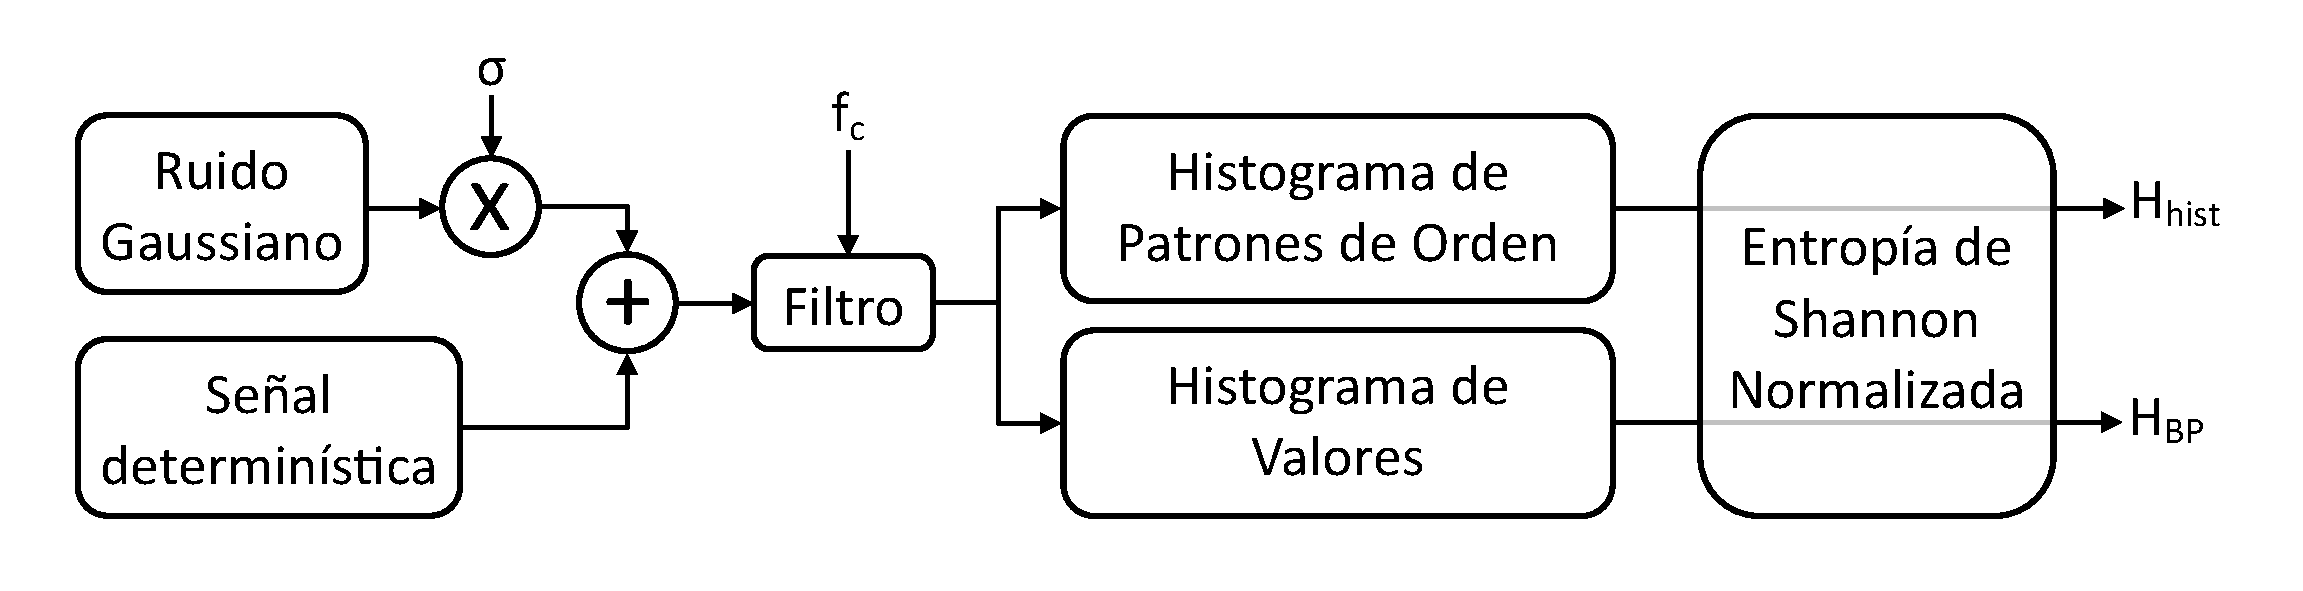
\includegraphics [width=0.99\textwidth]{FlowChart}
\caption {Diagrama de flujo del experimento.}\label{fig:flowchart}
\end{figure}

Para evaluar la contribución de cada componente espectral a las entropías, se evaluaron dos filtros.
Primero se aplicó un filtro elíptico de orden $10$ con ripple pasabanda de $0,5 dB$, ripple en la banda de rechazo de $100 dB$ y frecuencia de corte variable $f_c$, en la Figura \ref{fig:filtroellip} se muestra su respuesta en ganancia (Figura \ref{subfig:filtroellip_amplitud}) y fase (Figura \ref{subfig:filtroellip_frecuencia}) para el caso de $f_c=0,5$. De esta forma se logra un filtrado lo suficientemente abrupto como para considerar que a medida que se barren distintas frecuencias de corte se eliminan componentes espectrales individualmente.
Los resultados de este filtrado se compararon con los resultados de un filtro ideal (Figura \ref{fig:filtroideal}), que consiste en una máscara aplicada a la transformada de fourier de la señal a filtrar, de esta manera se consigue el espectro de la señal filtrada, el cual es antitransformado para recuperar la versión filtrada en las muestras. El diagrama de este filtro puede verse en la Figura \ref{subfig:filtroideal_diagrama}. Este procedimiento equivale a un filtrado ideal sin retardo, por lo que el bode de amplitud es $0dB$ en la banda de paso y $-\infty dB$ en la banda de rechazo (Figura \ref{subfig:filtroideal_diagrama}); la fase $\omega\tau=0$ es lineal con pendiente nula (Figura \ref{subfig:filtroideal_frecuencia}).
%
\begin{figure}[h]
    \centering
    \begin{subfigure}[t]{.49\textwidth}
        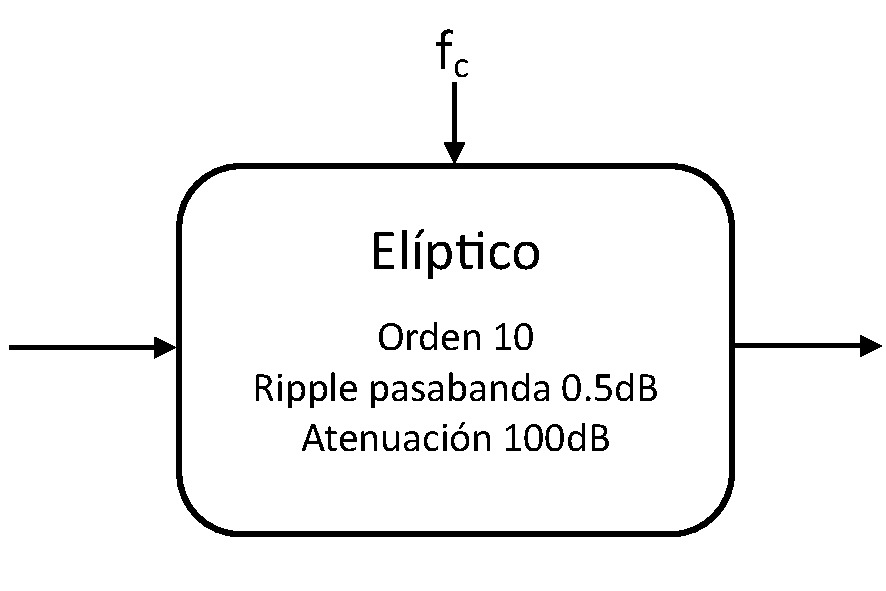
\includegraphics[width=\textwidth]{Ellip}
        \caption{Esquema}
        \label{subfig:filtroellip_diagrama}
    \end{subfigure}
    ~ %add desired spacing between images, e. g. ~, \quad, \qquad, \hfill etc. 
      %(or a blank line to force the subfigure onto a new line)
    \begin{subfigure}[t]{.49\textwidth}
        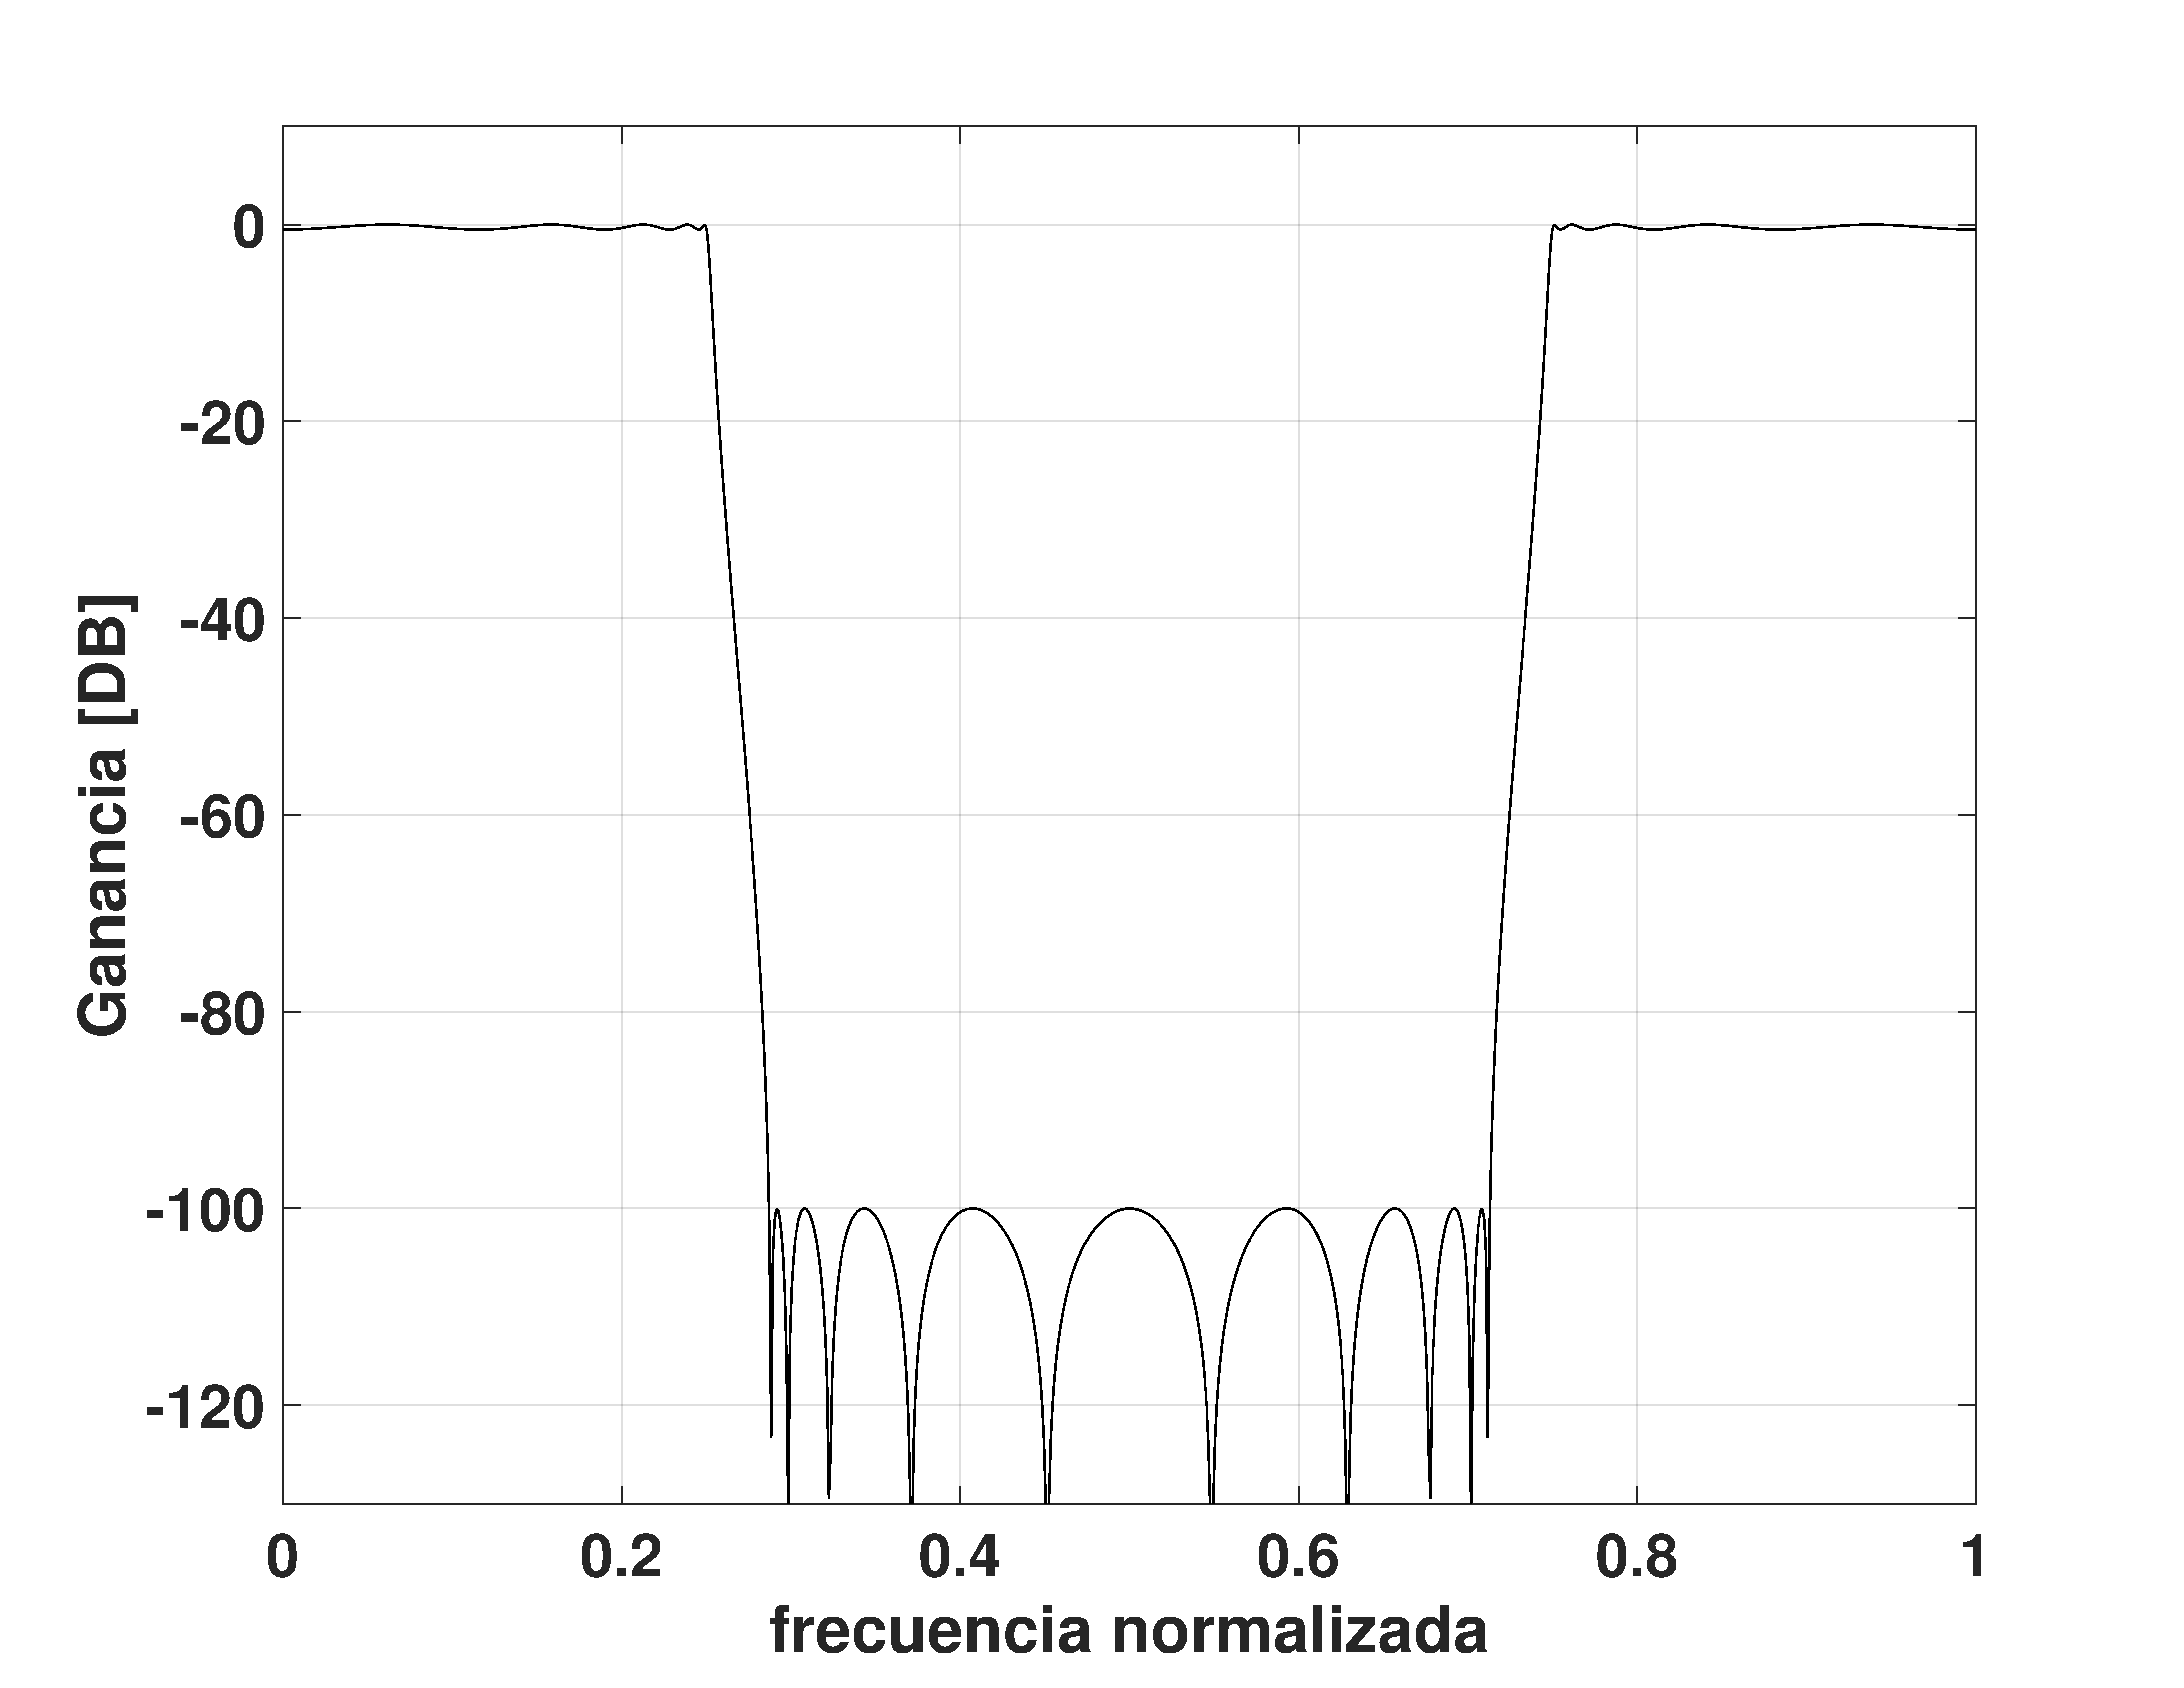
\includegraphics[width=\textwidth]{BodeEllip}
        \caption{Bode de ganancia}
        \label{subfig:filtroellip_amplitud}
    \end{subfigure}
    ~ %add desired spacing between images, e. g. ~, \quad, \qquad, \hfill etc. 
    %(or a blank line to force the subfigure onto a new line)
    \begin{subfigure}[t]{.49\textwidth}
        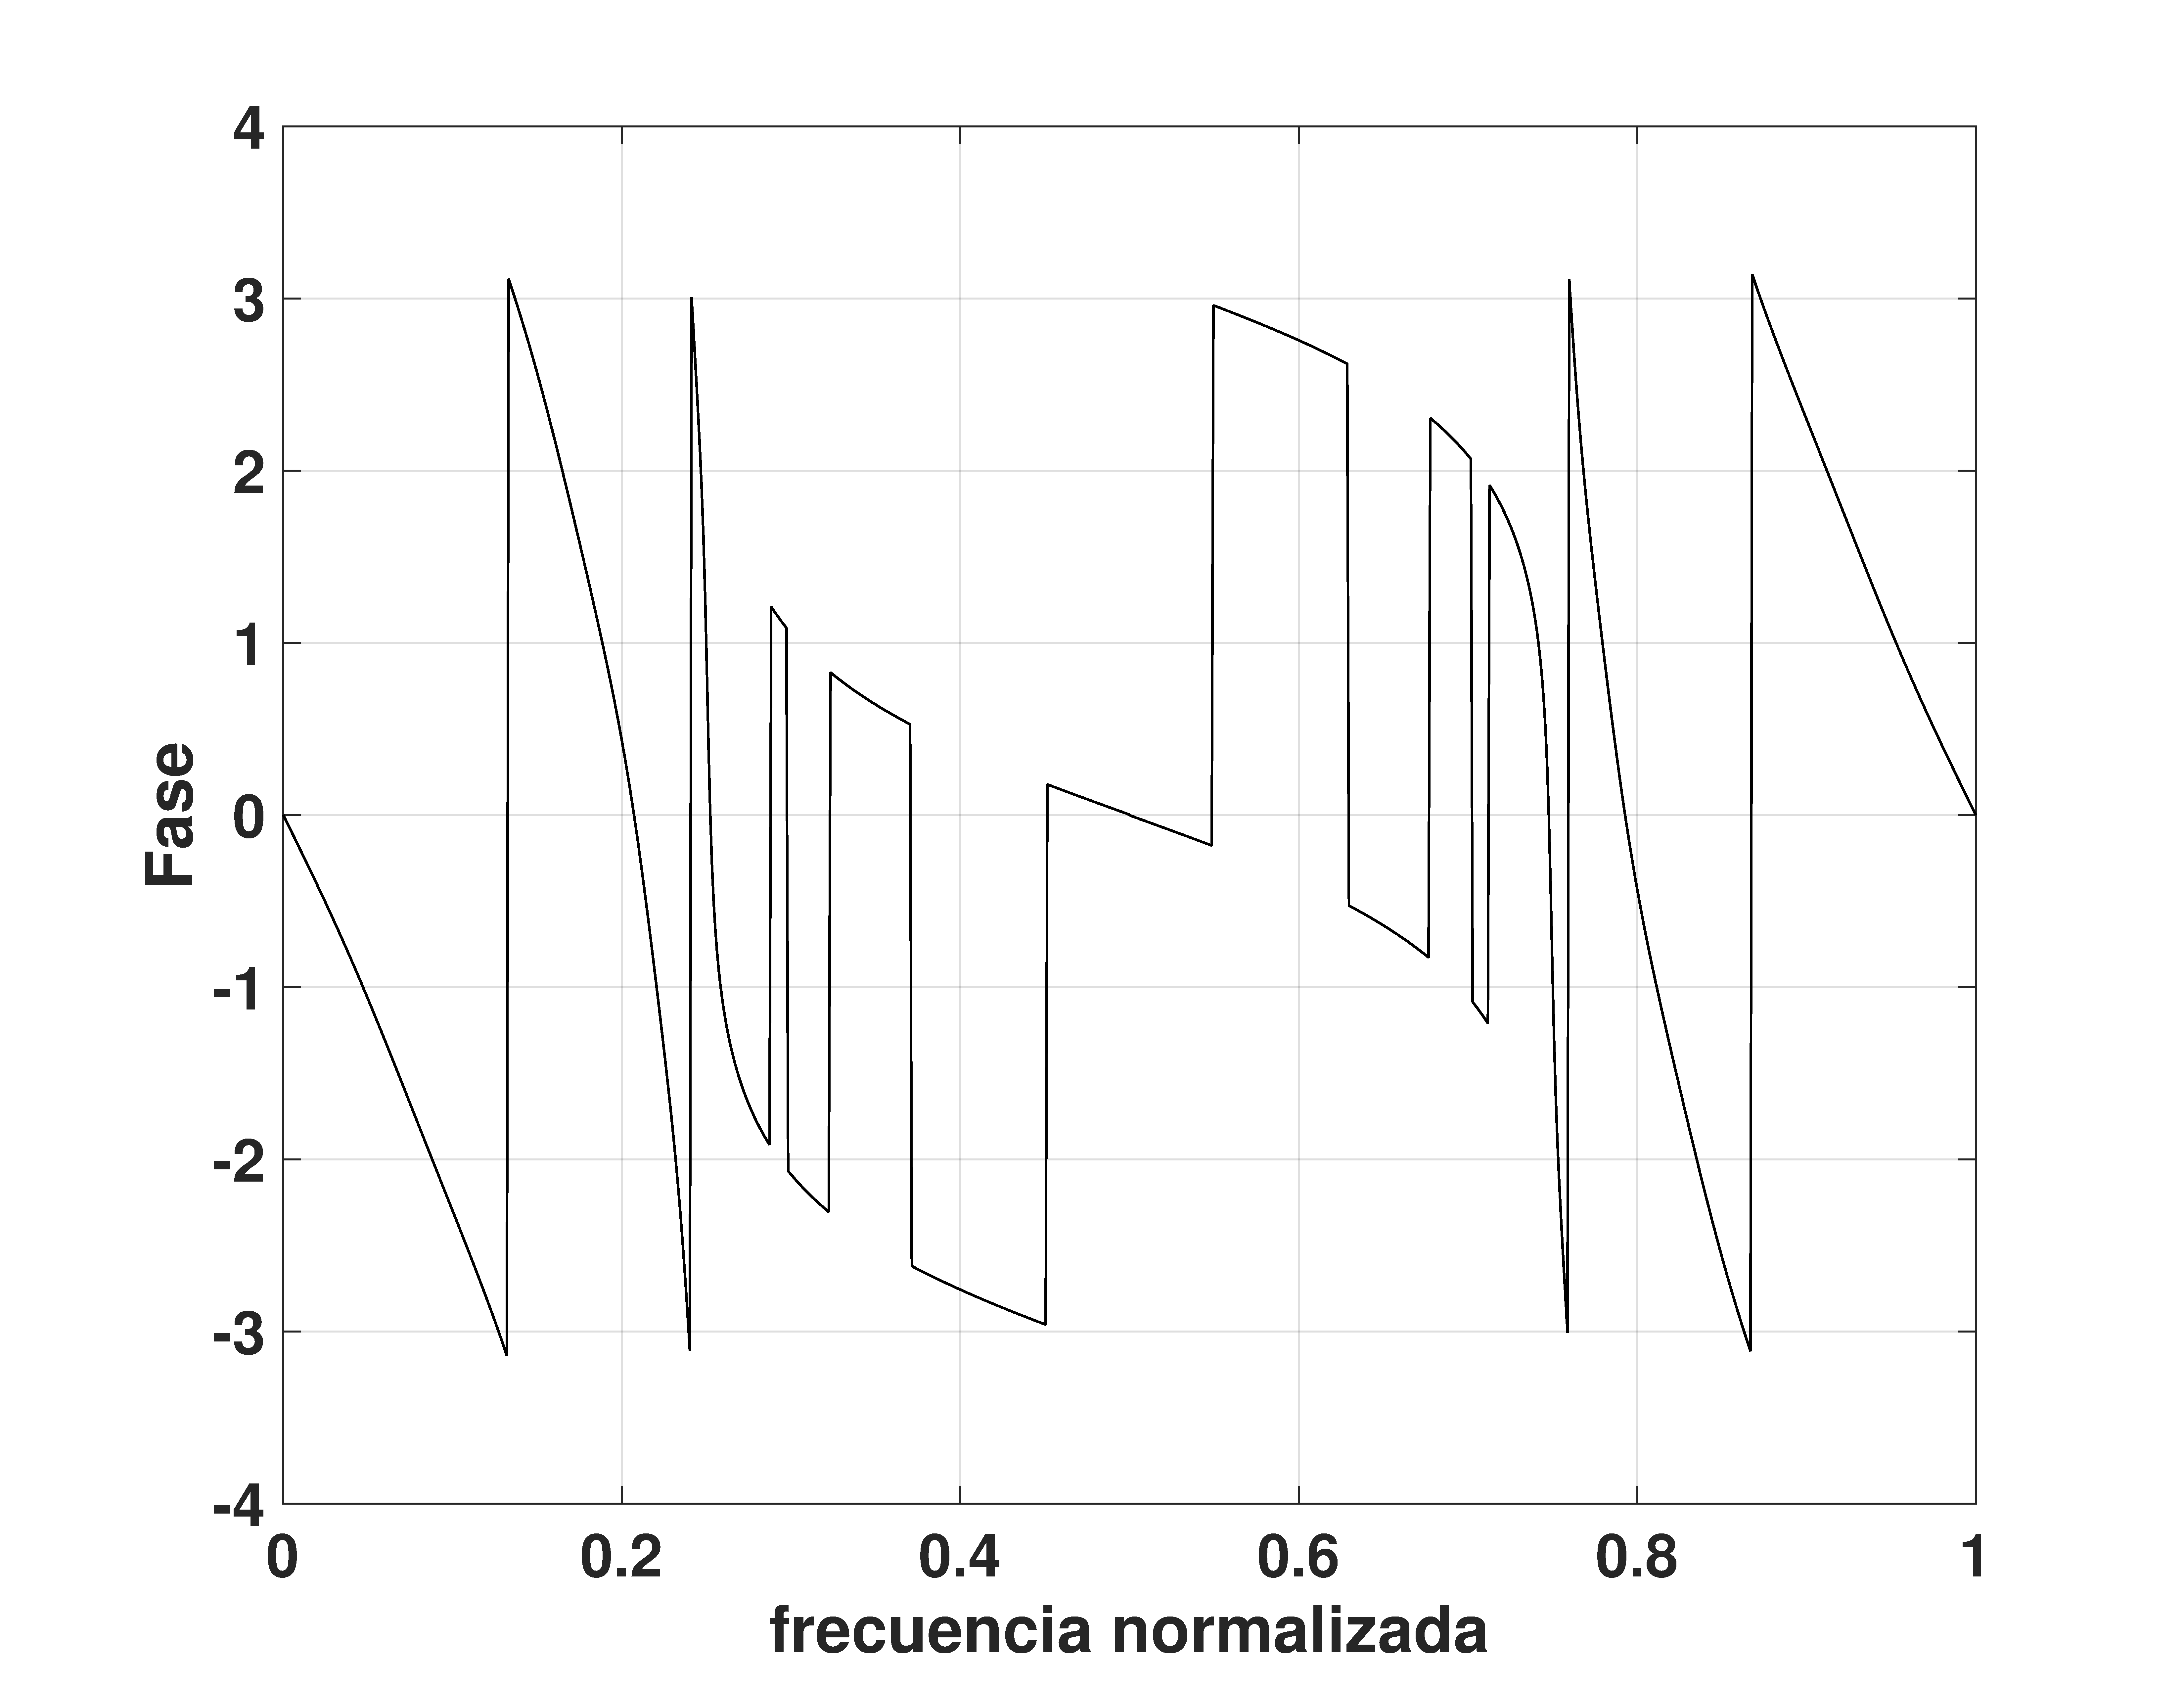
\includegraphics[width=\textwidth]{FreqEllip}
        \caption{Bode de fase}
        \label{subfig:filtroellip_frecuencia}
    \end{subfigure}
    \caption{Filtro elíptico.}\label{fig:filtroellip}
\end{figure}
%
\begin{figure}[h]
    \centering
    \begin{subfigure}[t]{.49\textwidth}
        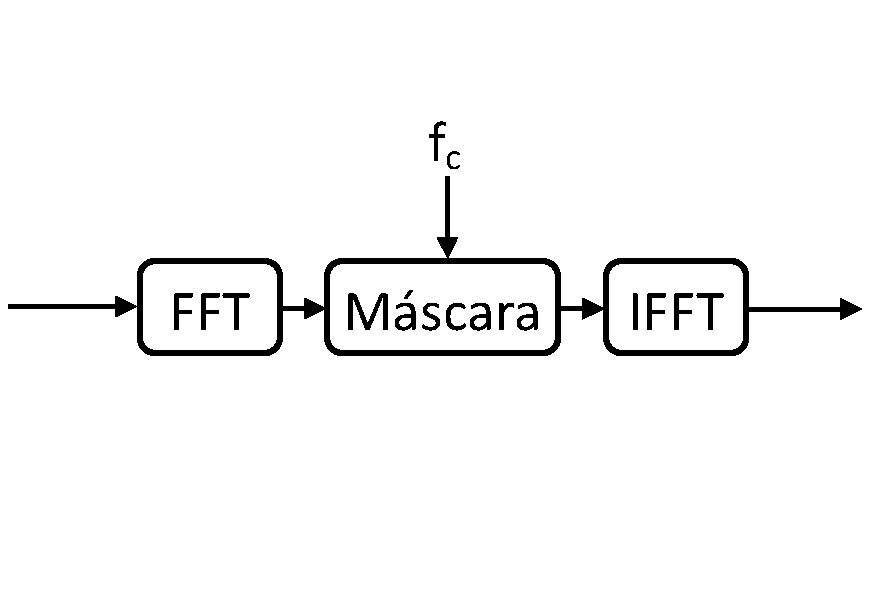
\includegraphics[width=\textwidth]{Ideal}
        \caption{Esquema}
        \label{subfig:filtroideal_diagrama}
    \end{subfigure}
    ~ %add desired spacing between images, e. g. ~, \quad, \qquad, \hfill etc. 
      %(or a blank line to force the subfigure onto a new line)
    \begin{subfigure}[t]{.49\textwidth}
        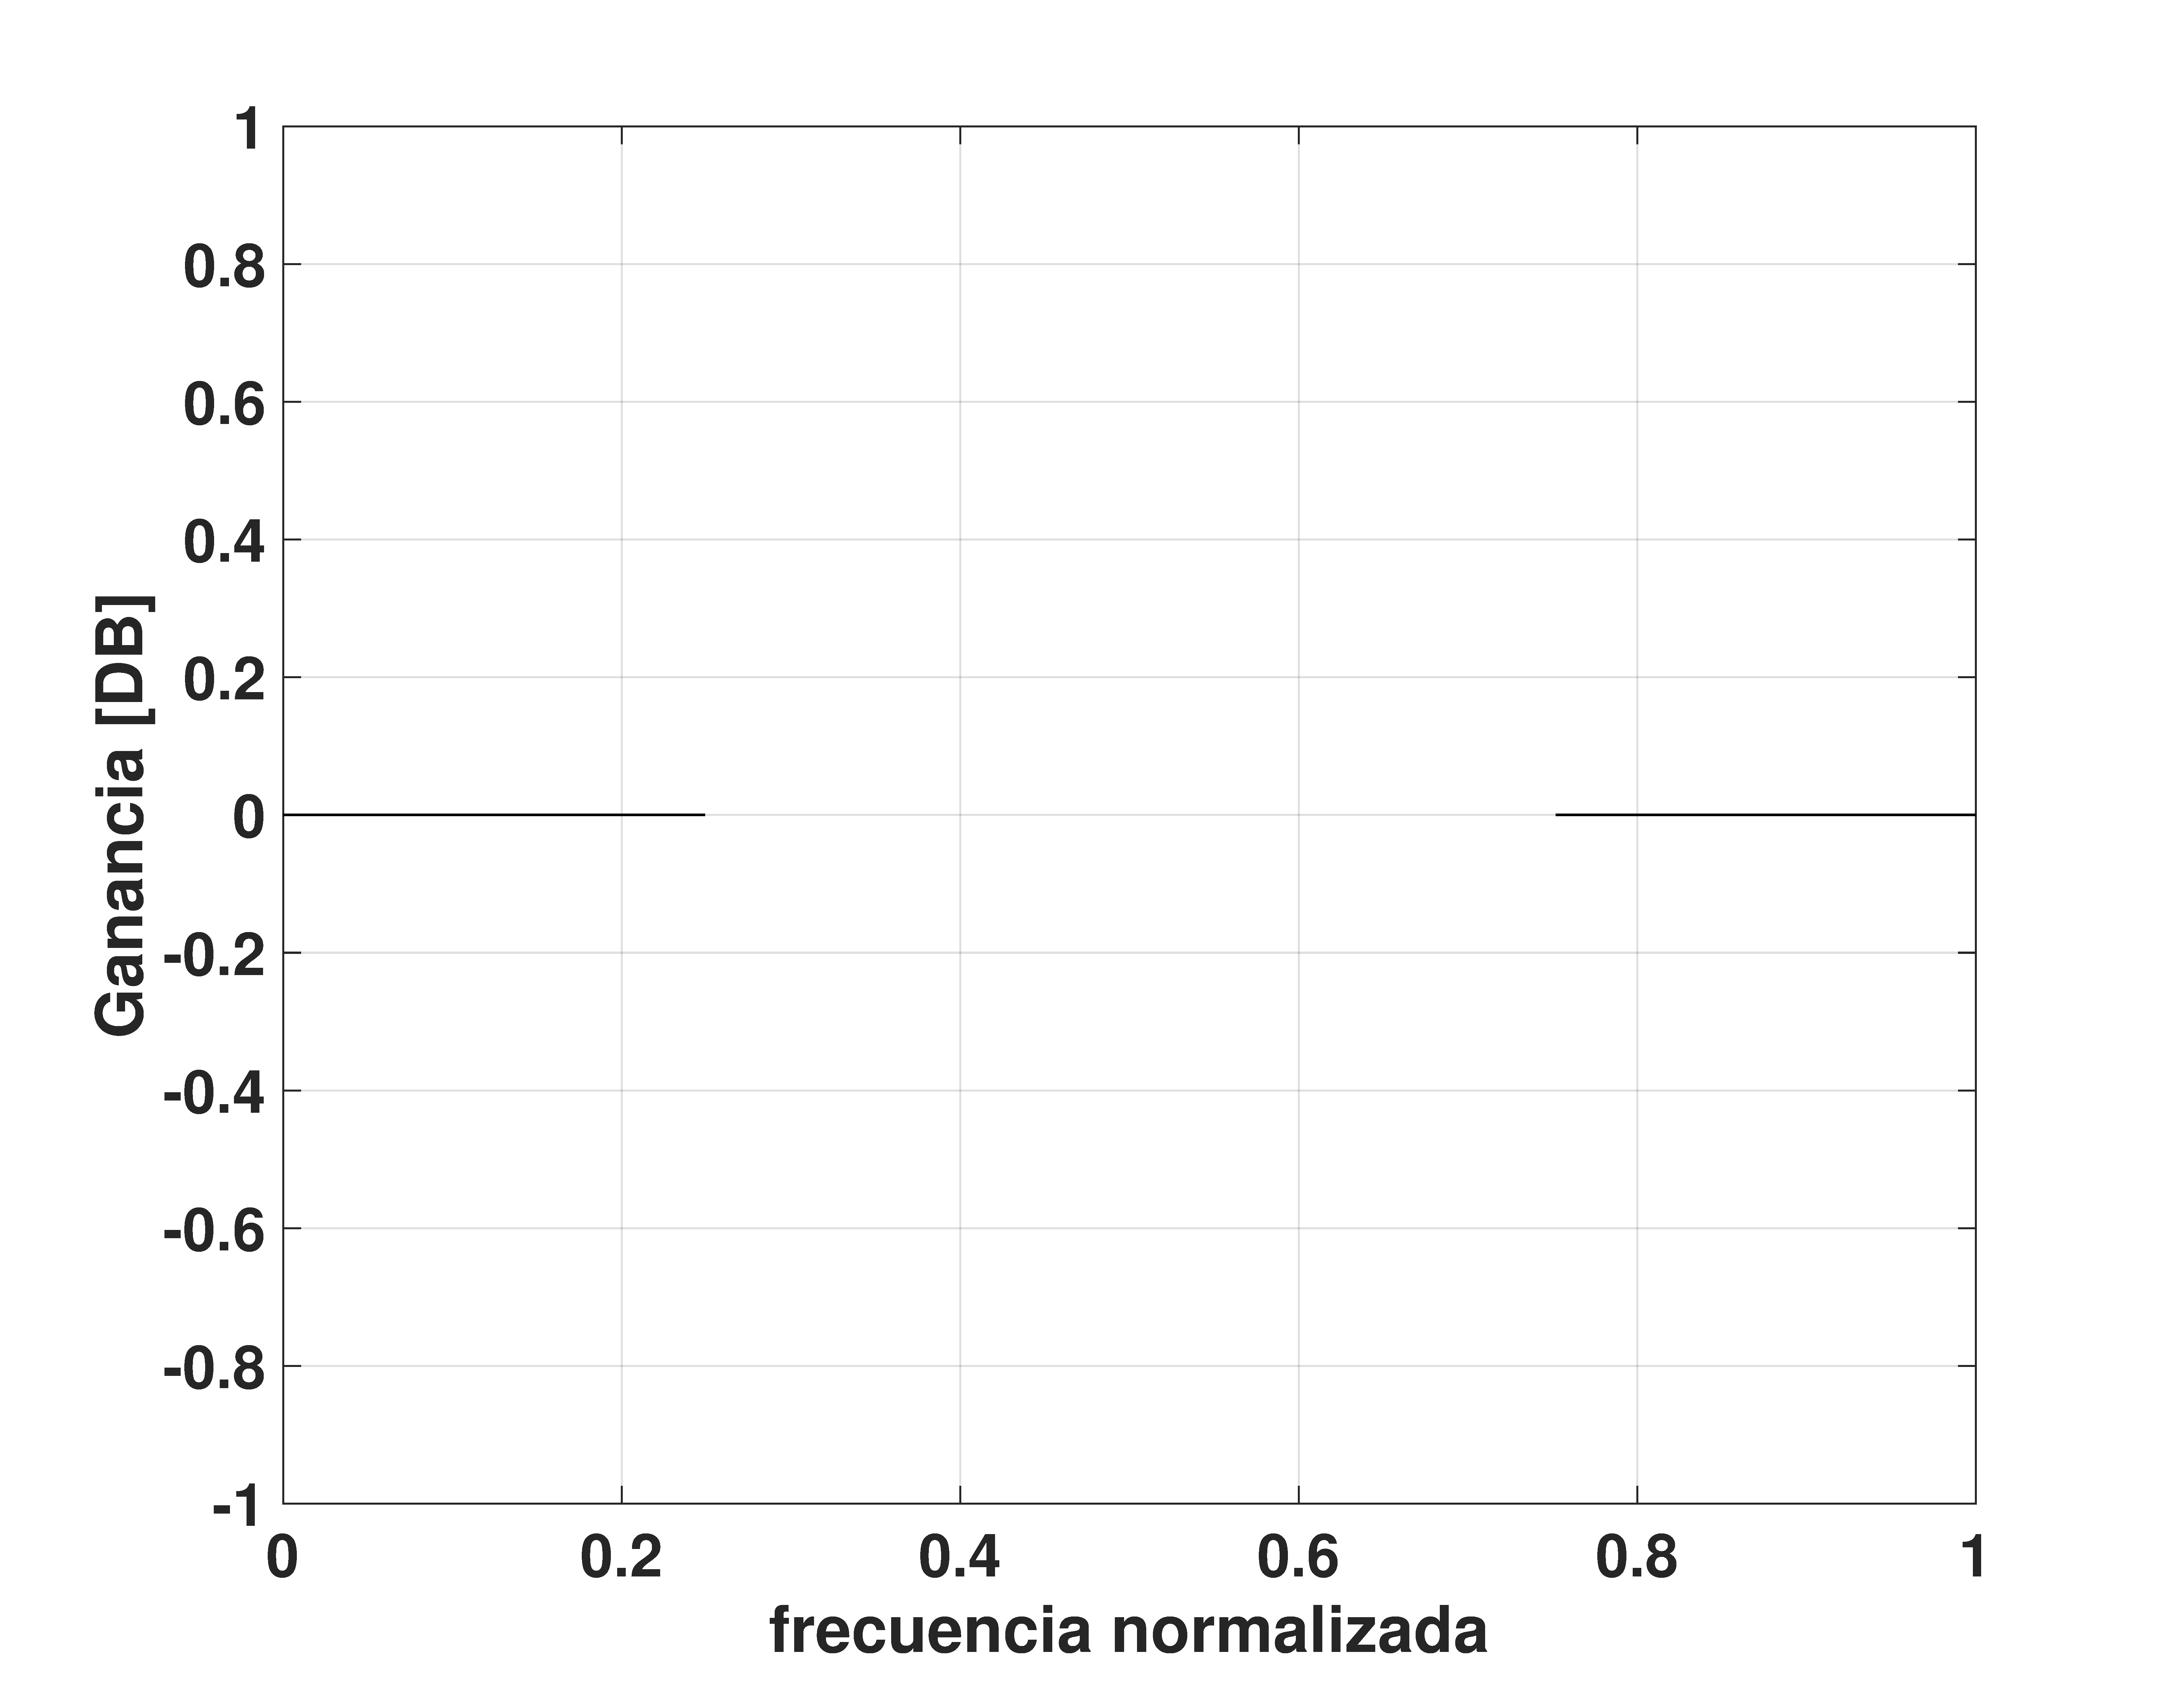
\includegraphics[width=\textwidth]{BodeIdeal}
        \caption{Bode de ganancia}
        \label{subfig:filtroideal_amplitud}
    \end{subfigure}
    ~ %add desired spacing between images, e. g. ~, \quad, \qquad, \hfill etc. 
    %(or a blank line to force the subfigure onto a new line)
    \begin{subfigure}[t]{.49\textwidth}
        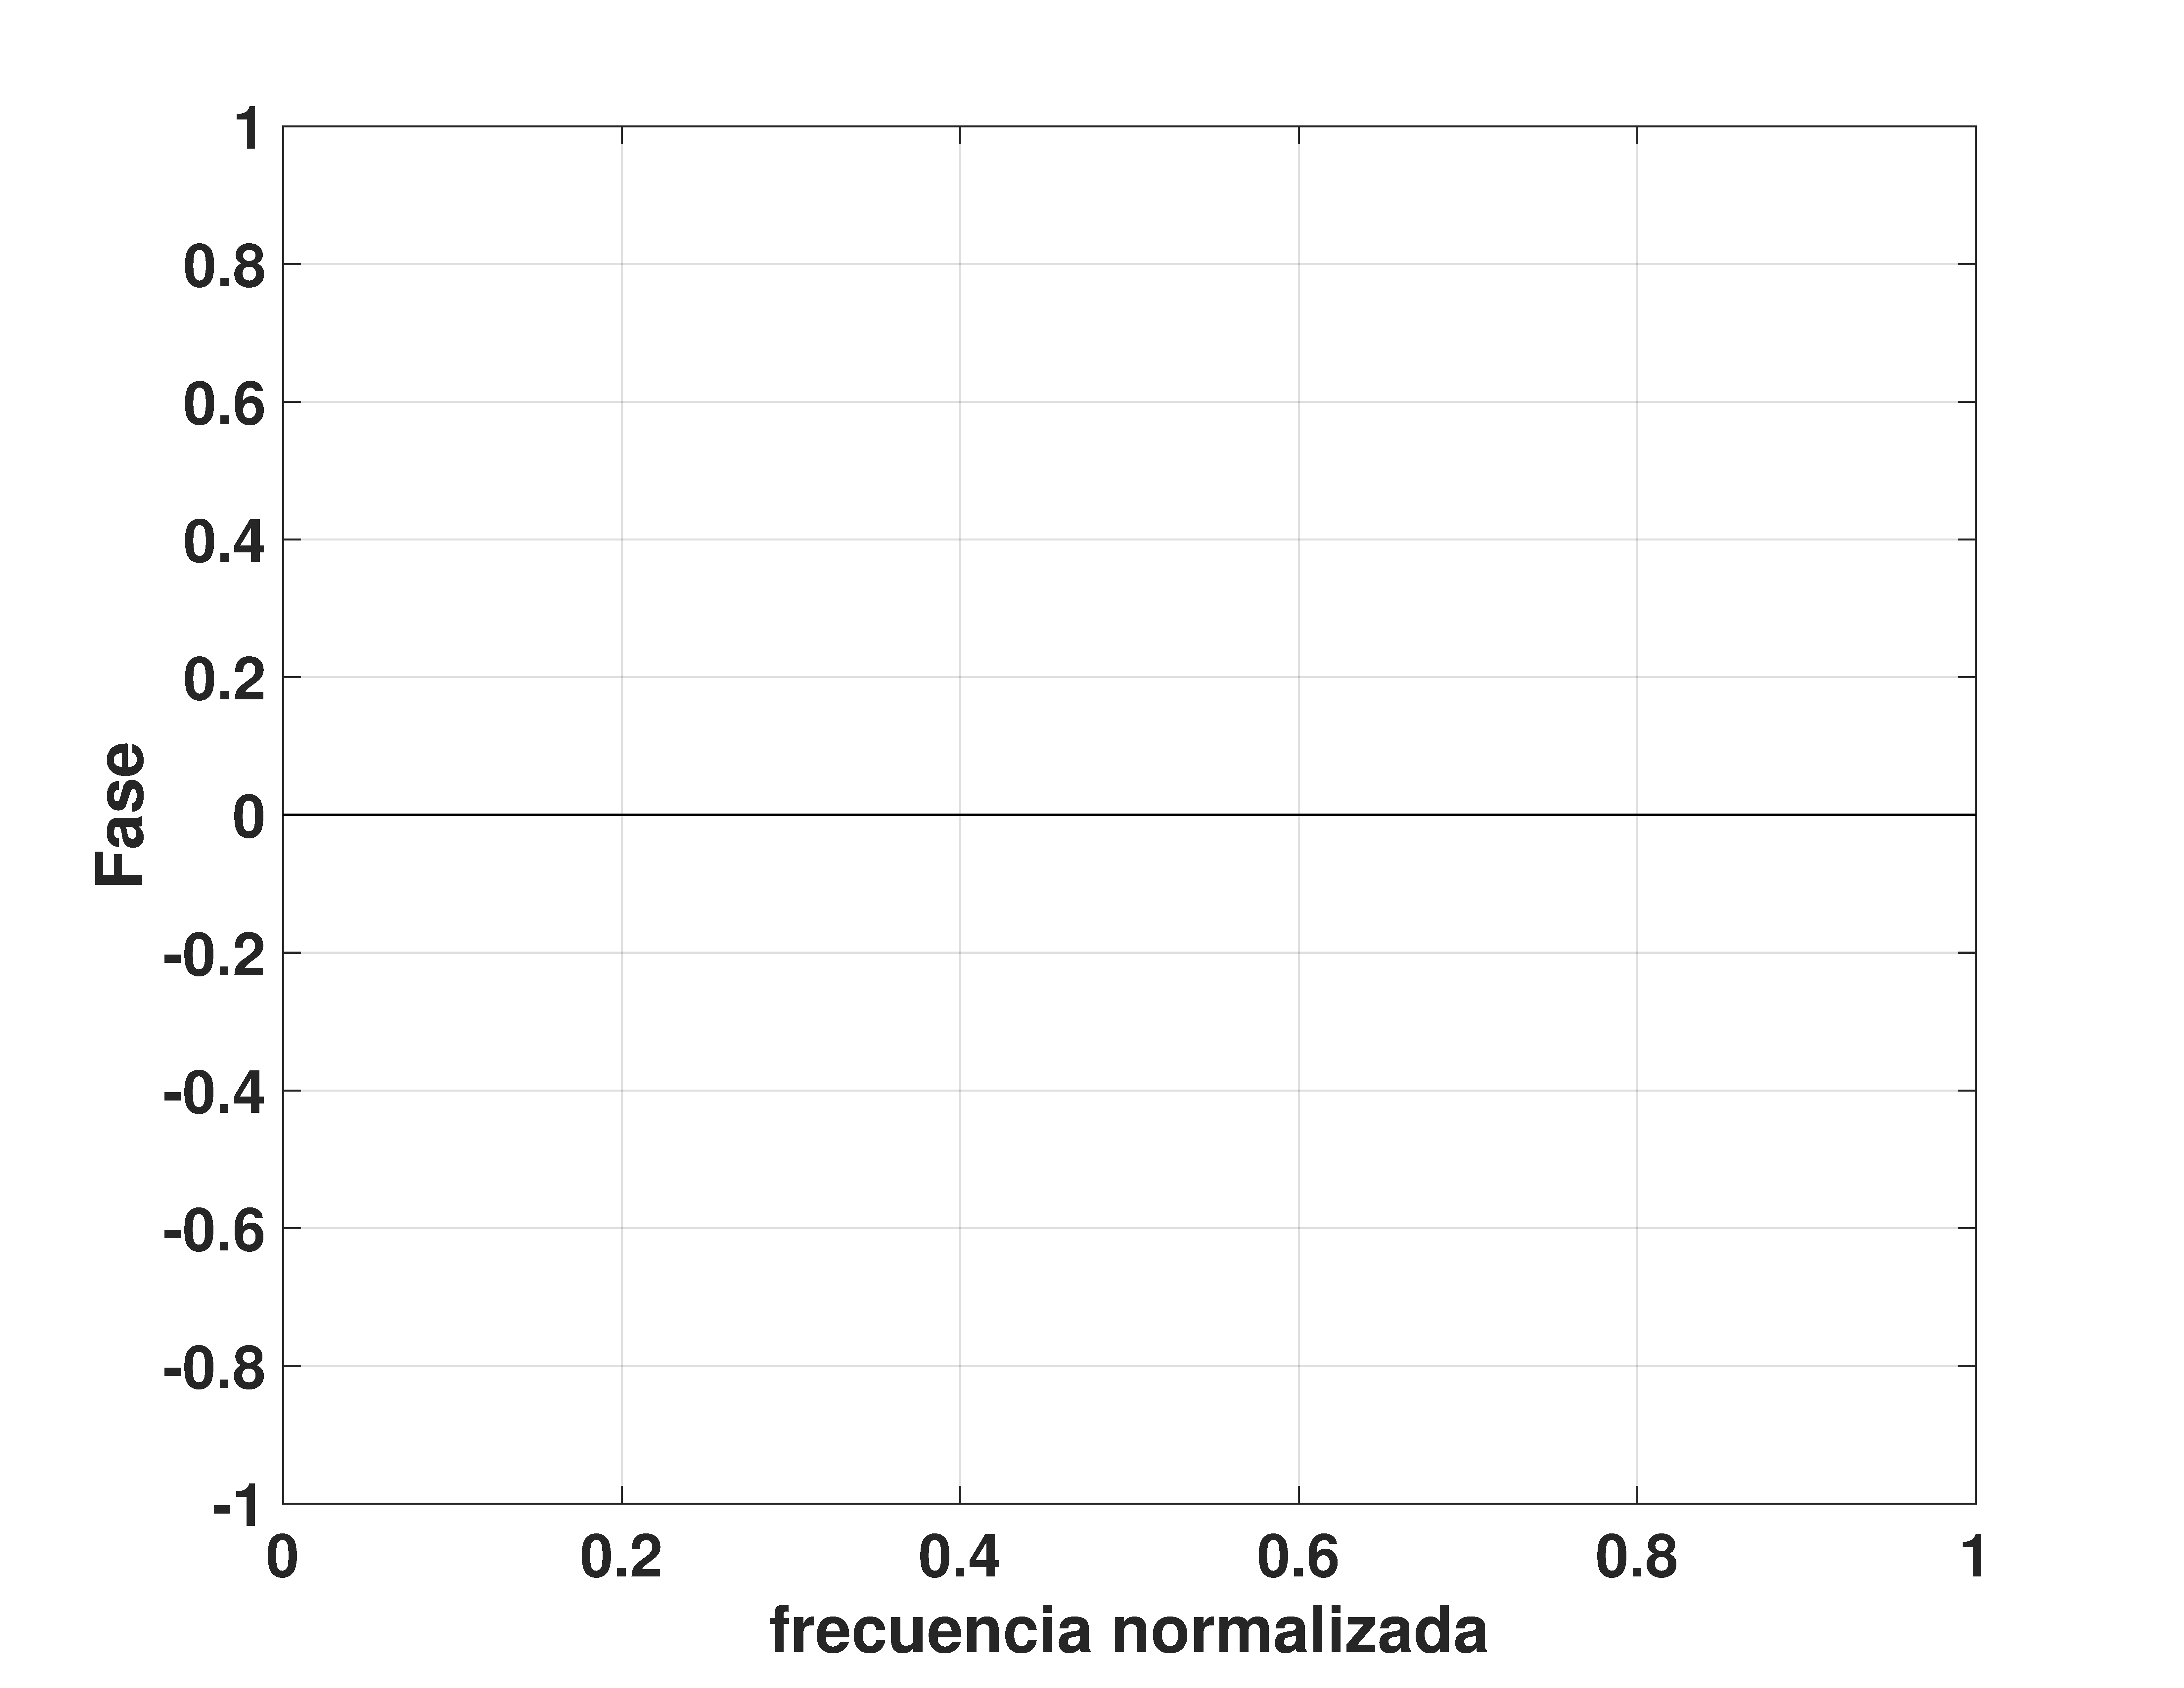
\includegraphics[width=\textwidth]{FreqIdeal}
        \caption{Bode de fase}
        \label{subfig:filtroideal_frecuencia}
    \end{subfigure}
    \caption{Filtro ideal.}\label{fig:filtroideal}
\end{figure}

Primero se aplicó una señal de ruido blanco gaussiano, es decir que la señal determinística es cero y la desviación estándar de la gaussiana unitaria.
En la Figura \ref{fig:ellip} se muestra el resultado de los cuantificadores a medida que se va barriendo la frecuencia de corte del filtro elíptico.
En la Figura \ref{subfig:ellip_Hhist} se muestra la entropía del histograma de valores $H_{hist}$, puede verse que su valor se mantiene constante alrededor de $0,9$ tanto para el filtro pasa-bajos (roja) como el pasa-altos (azul), este valor es el mismo que resulta de calcular la entropía del histograma de valores a la señal sin filtrar (resultado que se muestra con una línea punteada negra en el mismo gráfico). También puede verse que cuando la frecuencia de corte del filtro elíptico se acerca a los extremos el valor del cuantificador cae, en estas frecuencias el método numérico que calcula el vector filtrado diverge debido a la precisión finita.
En la Figura \ref{subfig:ellip_Hbp} se muestra la entropía de los patrones de orden, $H_{BP}$ se mantiene en valores bajos cuando el filtro (pasa-altos en azul y pasa-bajos en rojo) deja pasar pocas componentes espectrales. Luego, a medida que la frecuencia de corte deja pasar más componentes espectrales, el cuantificador tiende a $1$, que es justamente el valor que arroja cuando se ingresa con la señal sin filtrar (este valor está indicado con una línea punteada negra).
El cuantificador detecta los cambios en la forma de la señal a medida que es filtrada.
Por último, en el plano $H_{hist} - H_{BP}$ de la Figura \ref{subfig:ellip_HbpHhist} se compacta la información de ambos cuantificadores, aunque se pierde la noción de la frecuencia de corte.
%
\begin{figure}[h]
    \centering
    \begin{subfigure}[t]{.49\textwidth}
        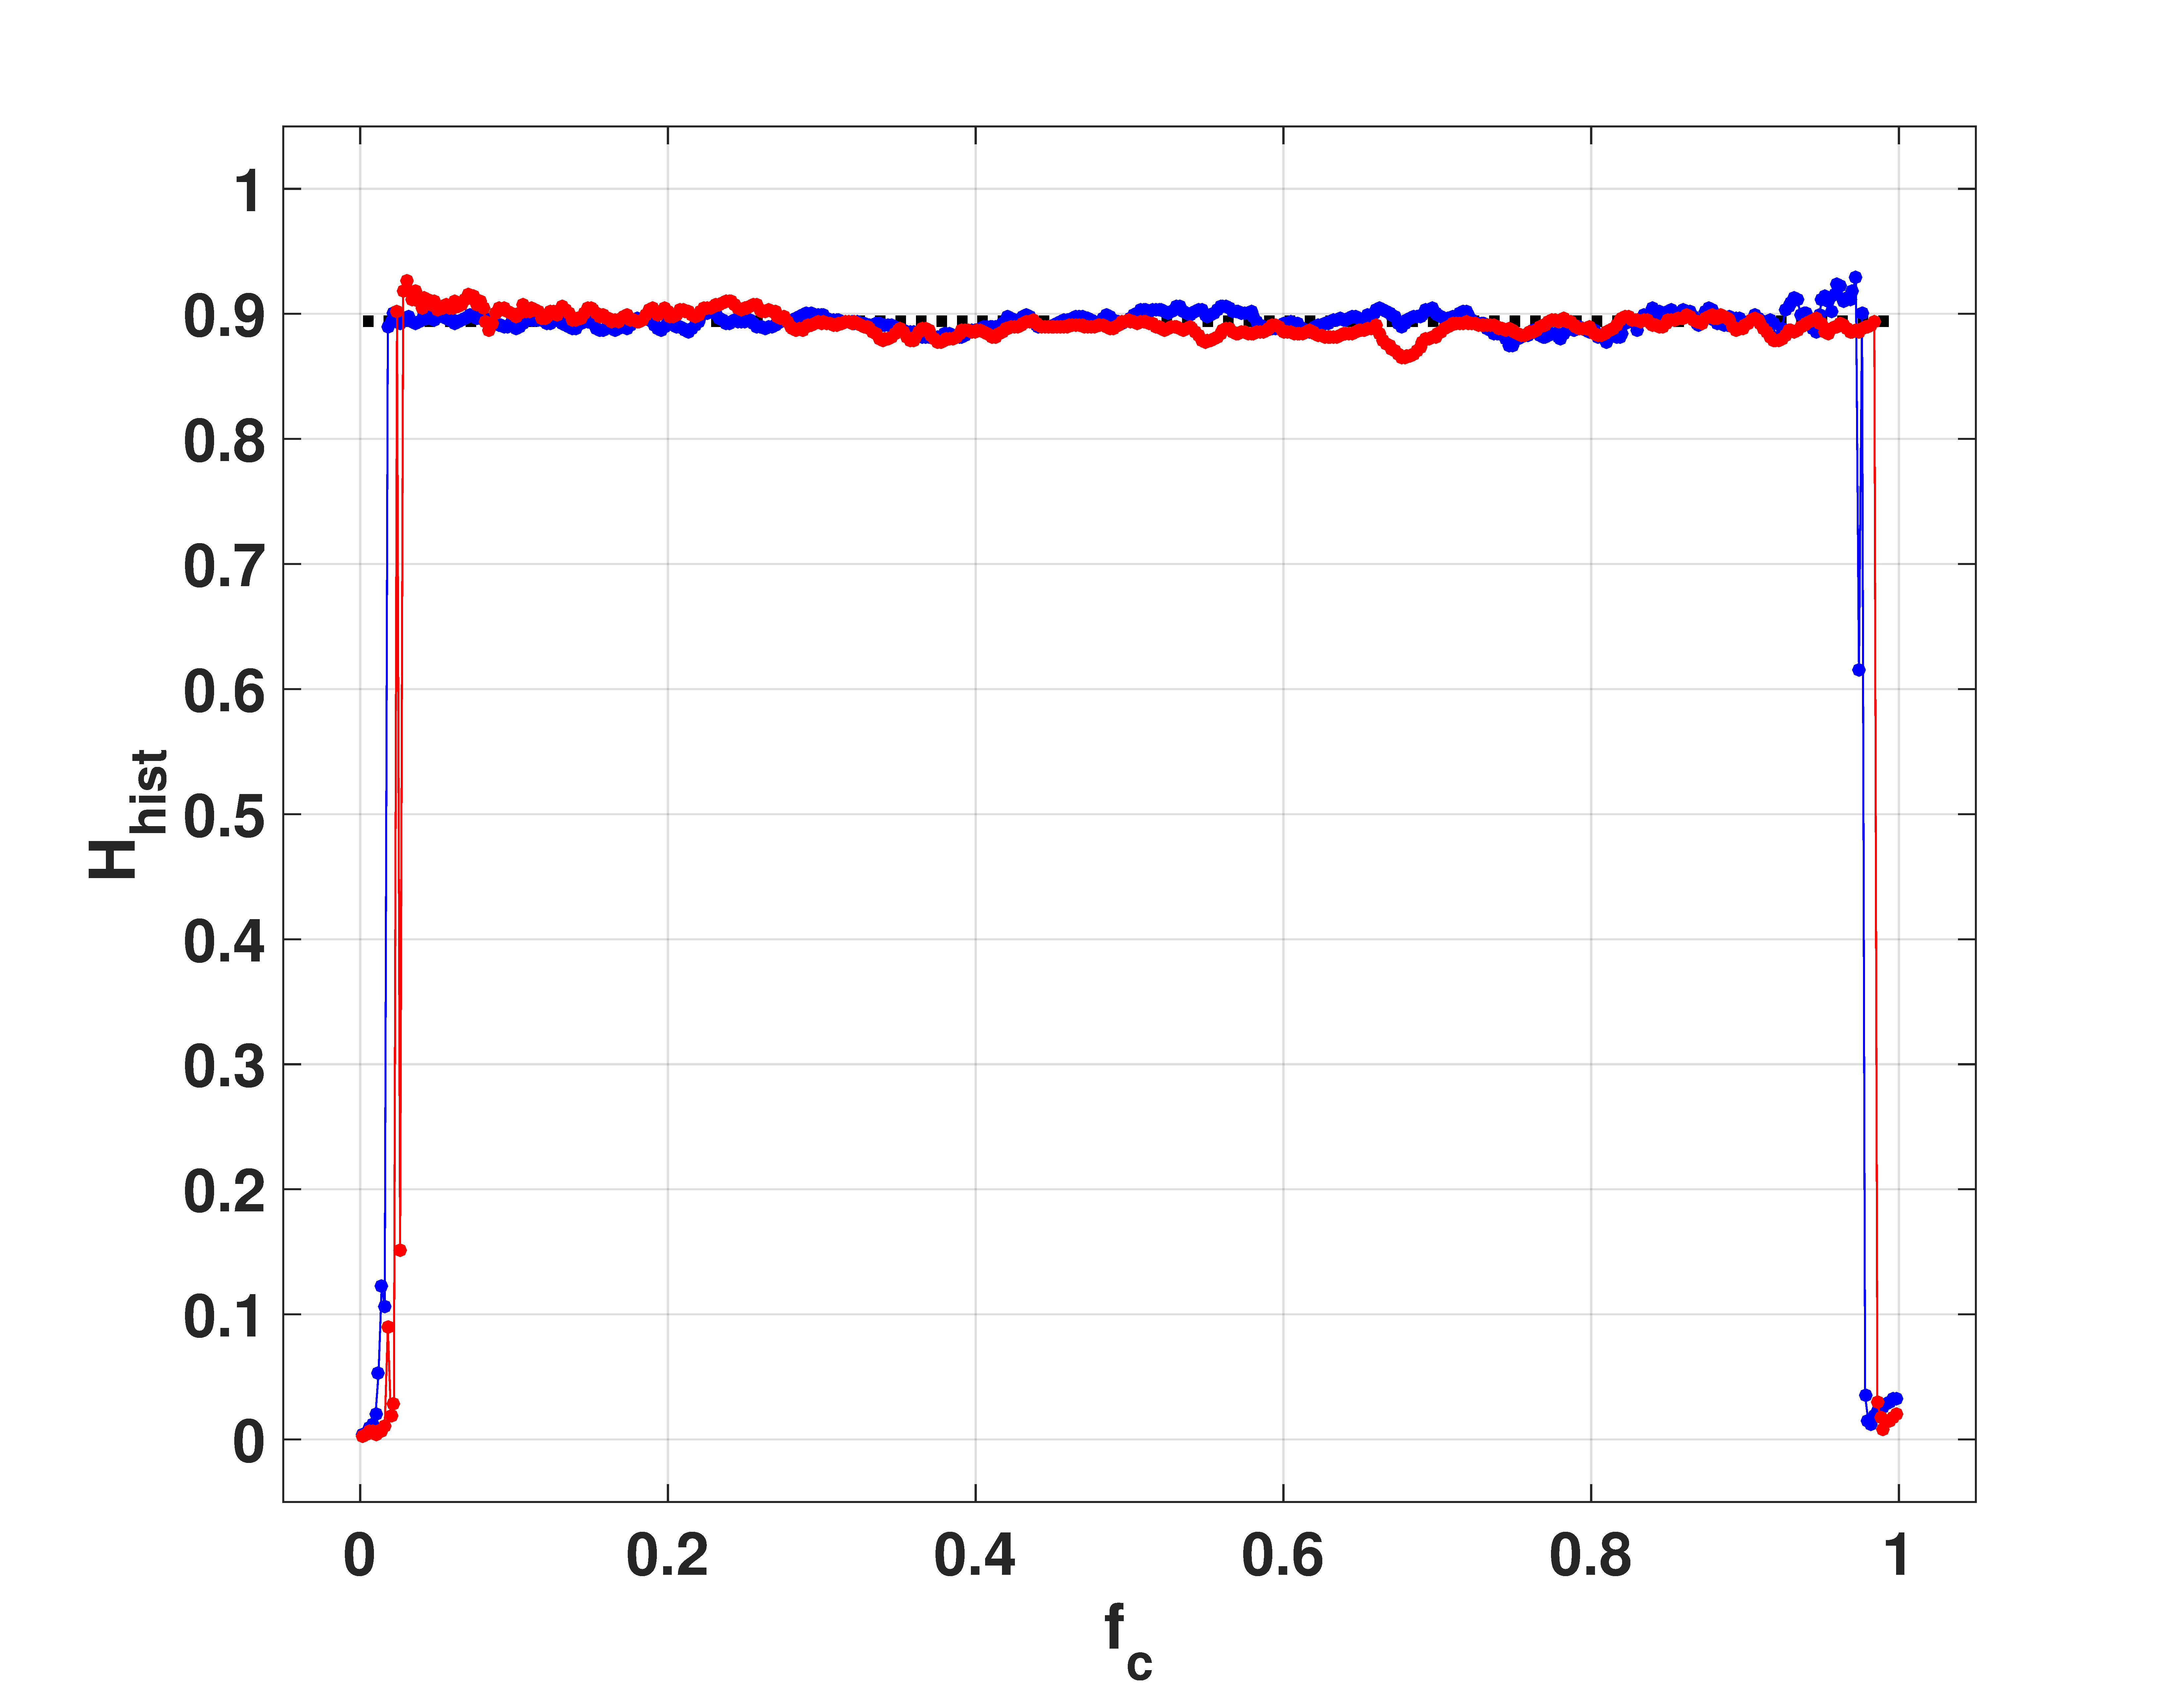
\includegraphics[width=\textwidth]{RuidoEllip_Hhist}
        \caption{Entropía de valores normalizada}
        \label{subfig:ellip_Hhist}
    \end{subfigure}
    ~ %add desired spacing between images, e. g. ~, \quad, \qquad, \hfill etc. 
      %(or a blank line to force the subfigure onto a new line)
    \begin{subfigure}[t]{.49\textwidth}
        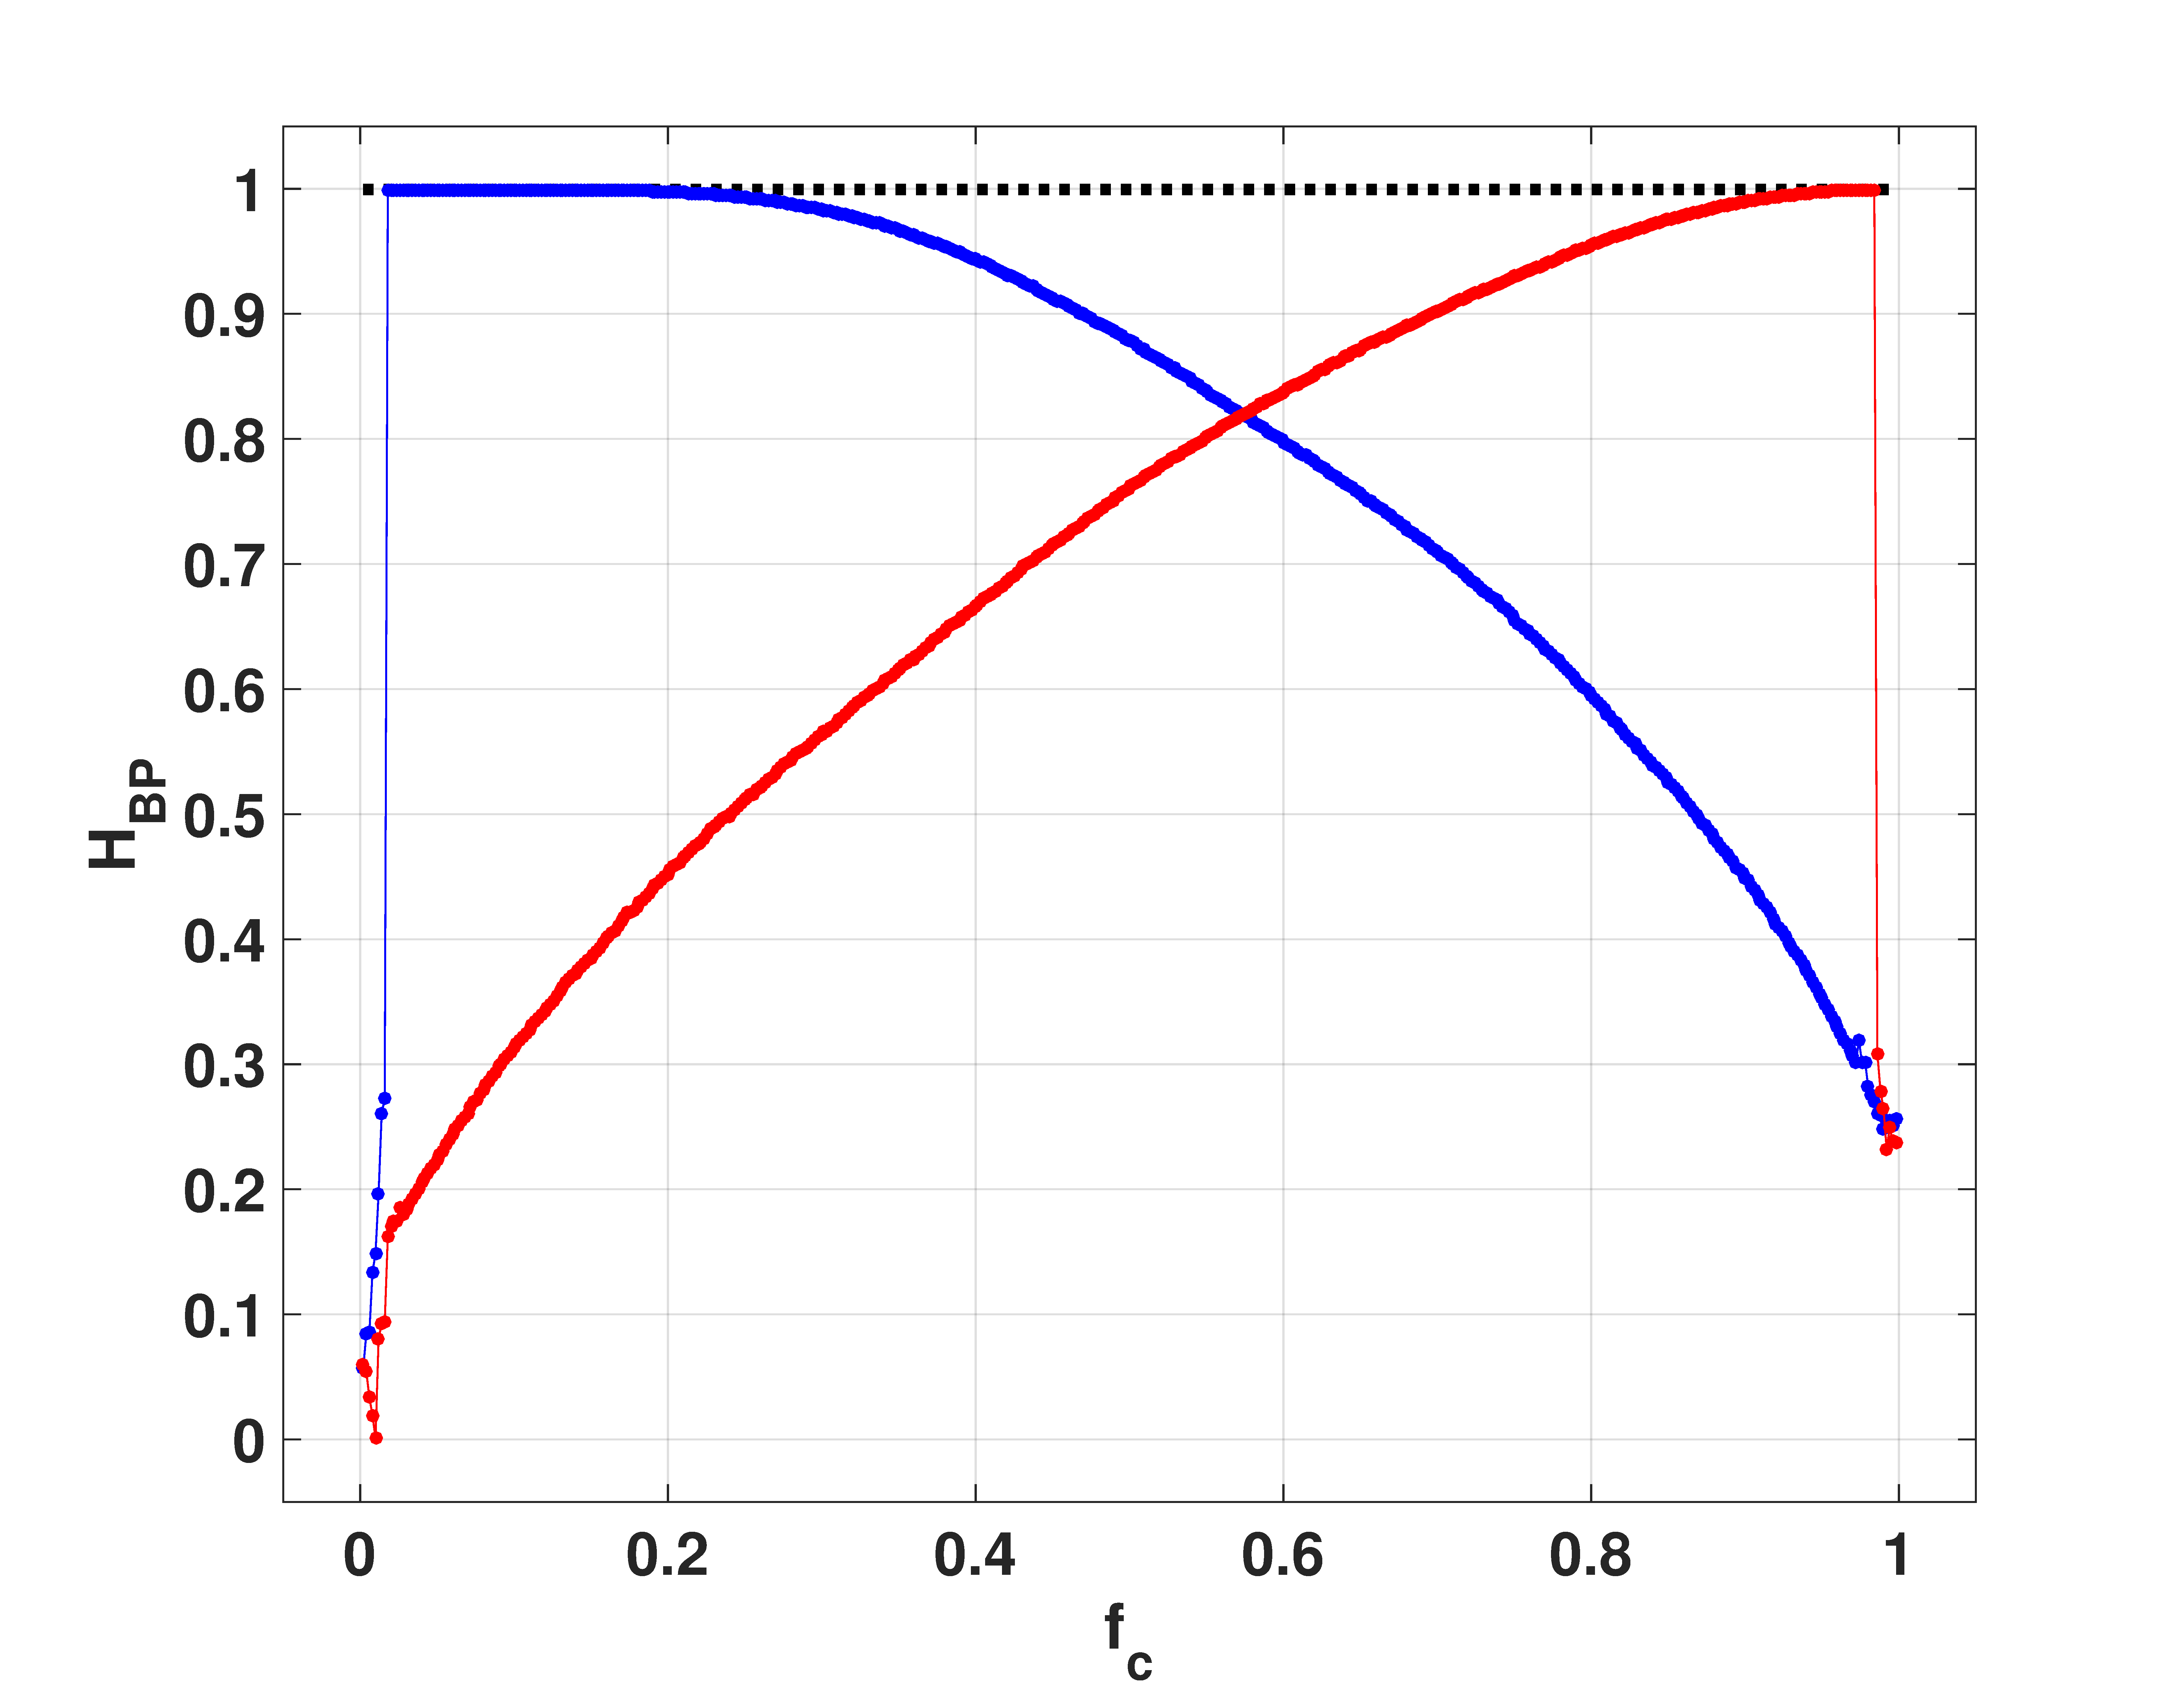
\includegraphics[width=\textwidth]{RuidoEllip_Hbp}
        \caption{Entropía de patrones de orden normalizada}
        \label{subfig:ellip_Hbp}
    \end{subfigure}
    ~ %add desired spacing between images, e. g. ~, \quad, \qquad, \hfill etc. 
    %(or a blank line to force the subfigure onto a new line)
    \begin{subfigure}[t]{.49\textwidth}
        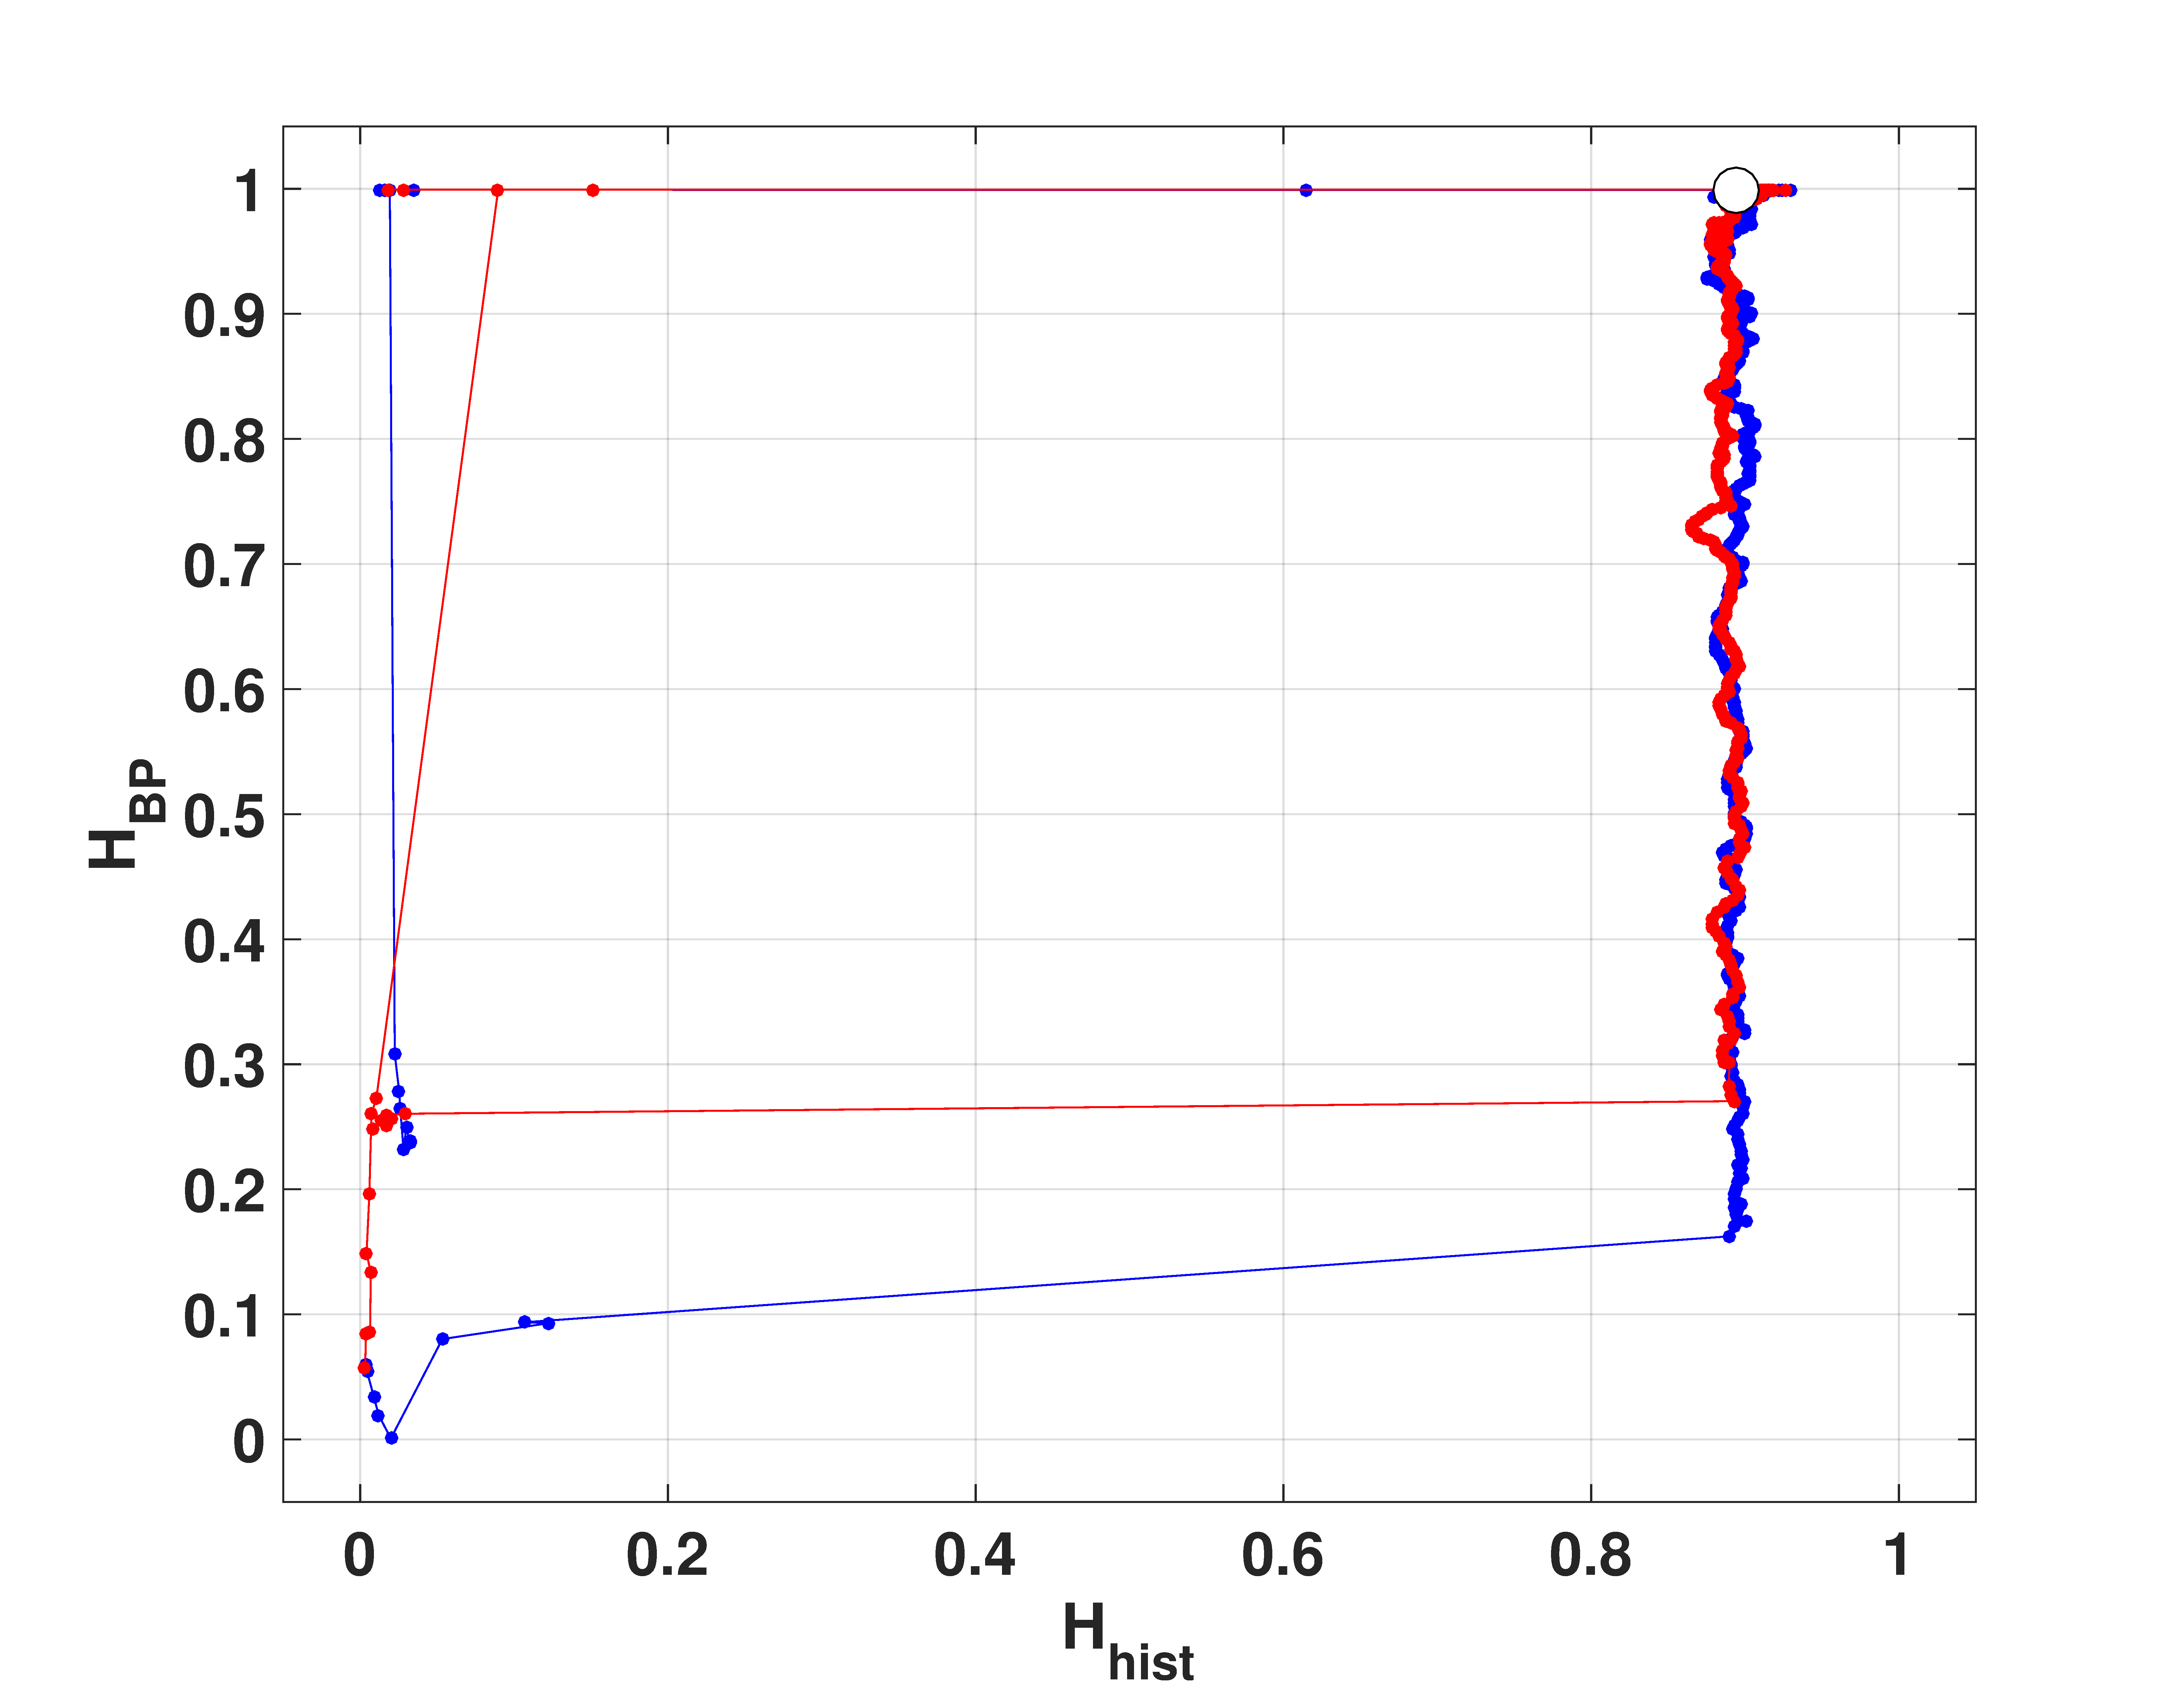
\includegraphics[width=\textwidth]{RuidoEllip_Hbp_Hhist}
        \caption{Plano doble entropía}
        \label{subfig:ellip_HbpHhist}
    \end{subfigure}
    \caption{Cuantificadores calculados sobre la salida del filtro elíptico cuando se ingresa con ruido blanco gaussiano.}\label{fig:ellip}
\end{figure}

En la Figura \ref{fig:ideal} se muestran los resultados del mismo procedimiento pero cuando se aplica un filtro ideal.
El comportamiento de los cuantificadores es igual al del filtro elíptico en todos los casos con la diferencia que el método no diverge cuando $f_c\to1$ o $f_c\to0$.
Pueden verse por lo tanto los valores que arrojan los cuantificadores en los extremos de la frecuencia de corte.
La entropía no causal de la Figura \ref{subfig:ideal_Hhist} aumenta levemente en los extremos, en donde el histograma de valores deja de tener una distribución gaussiana y se aplana levemente.
También puede verse en la Figura \ref{subfig:ideal_Hbp} que la entropía de valores $H_{BP}\to0,15$ cuando $f_c\to0$ para el pasa-bajos (rojo) y para el pasa-altos (azul) $H_{BP}\to0,22$ cuando $f_c\to1$.
En este caso es fácil comparar la sensibilidad al filtrado de ambos cuantificadores, en el plano doble entropía de la Figura \ref{subfig:ideal_HbpHhist}.
El círculo blanco muestra la posición en este plano cuando ningún filtro es aplicado, podemos ver que el apartamiento en el eje vertical aumenta a medida que la serie es filtrada, mientras que no se aparta en el sentido horizontal.
Esto muestra que la sensibilidad al filtrado de $H_{BP}$ es mucho mayor que la de $H_{hist}$.
%
\begin{figure}[h]
    \centering
    \begin{subfigure}[t]{.49\textwidth}
        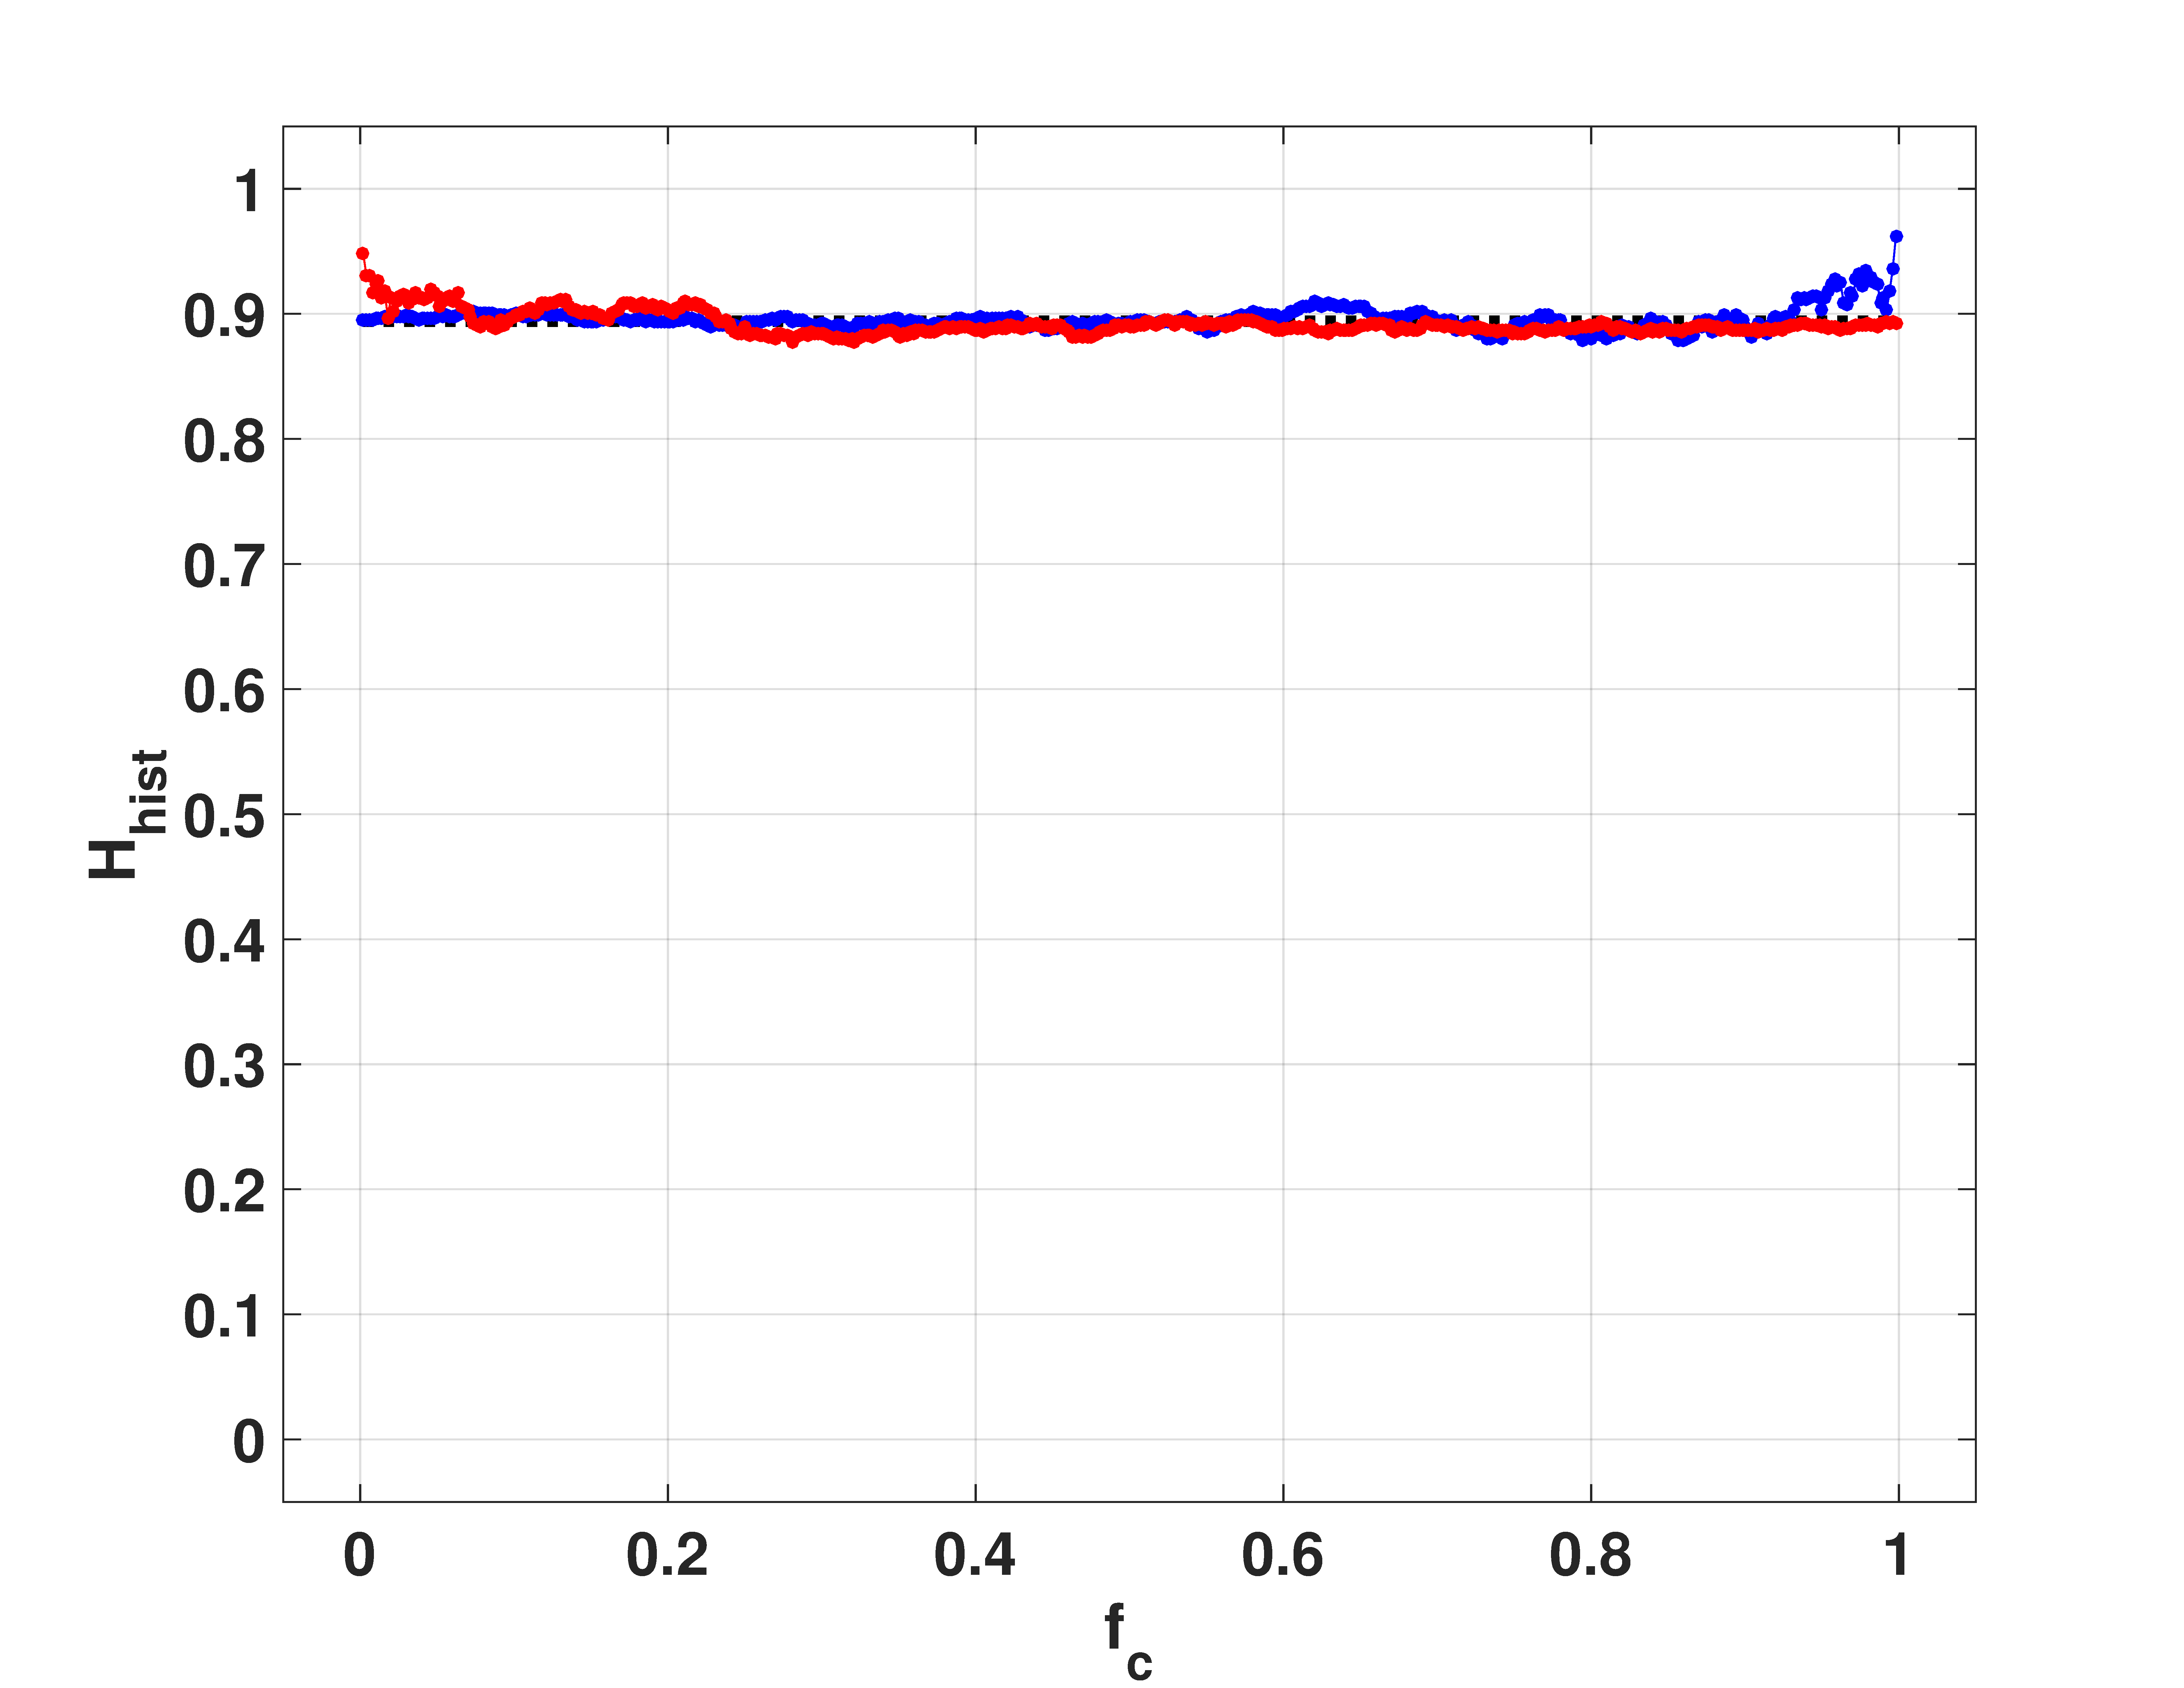
\includegraphics[width=\textwidth]{Ruido_Hhist}
        \caption{Entropía de valores normalizada}
        \label{subfig:ideal_Hhist}
    \end{subfigure}
    ~ %add desired spacing between images, e. g. ~, \quad, \qquad, \hfill etc. 
      %(or a blank line to force the subfigure onto a new line)
    \begin{subfigure}[t]{.49\textwidth}
        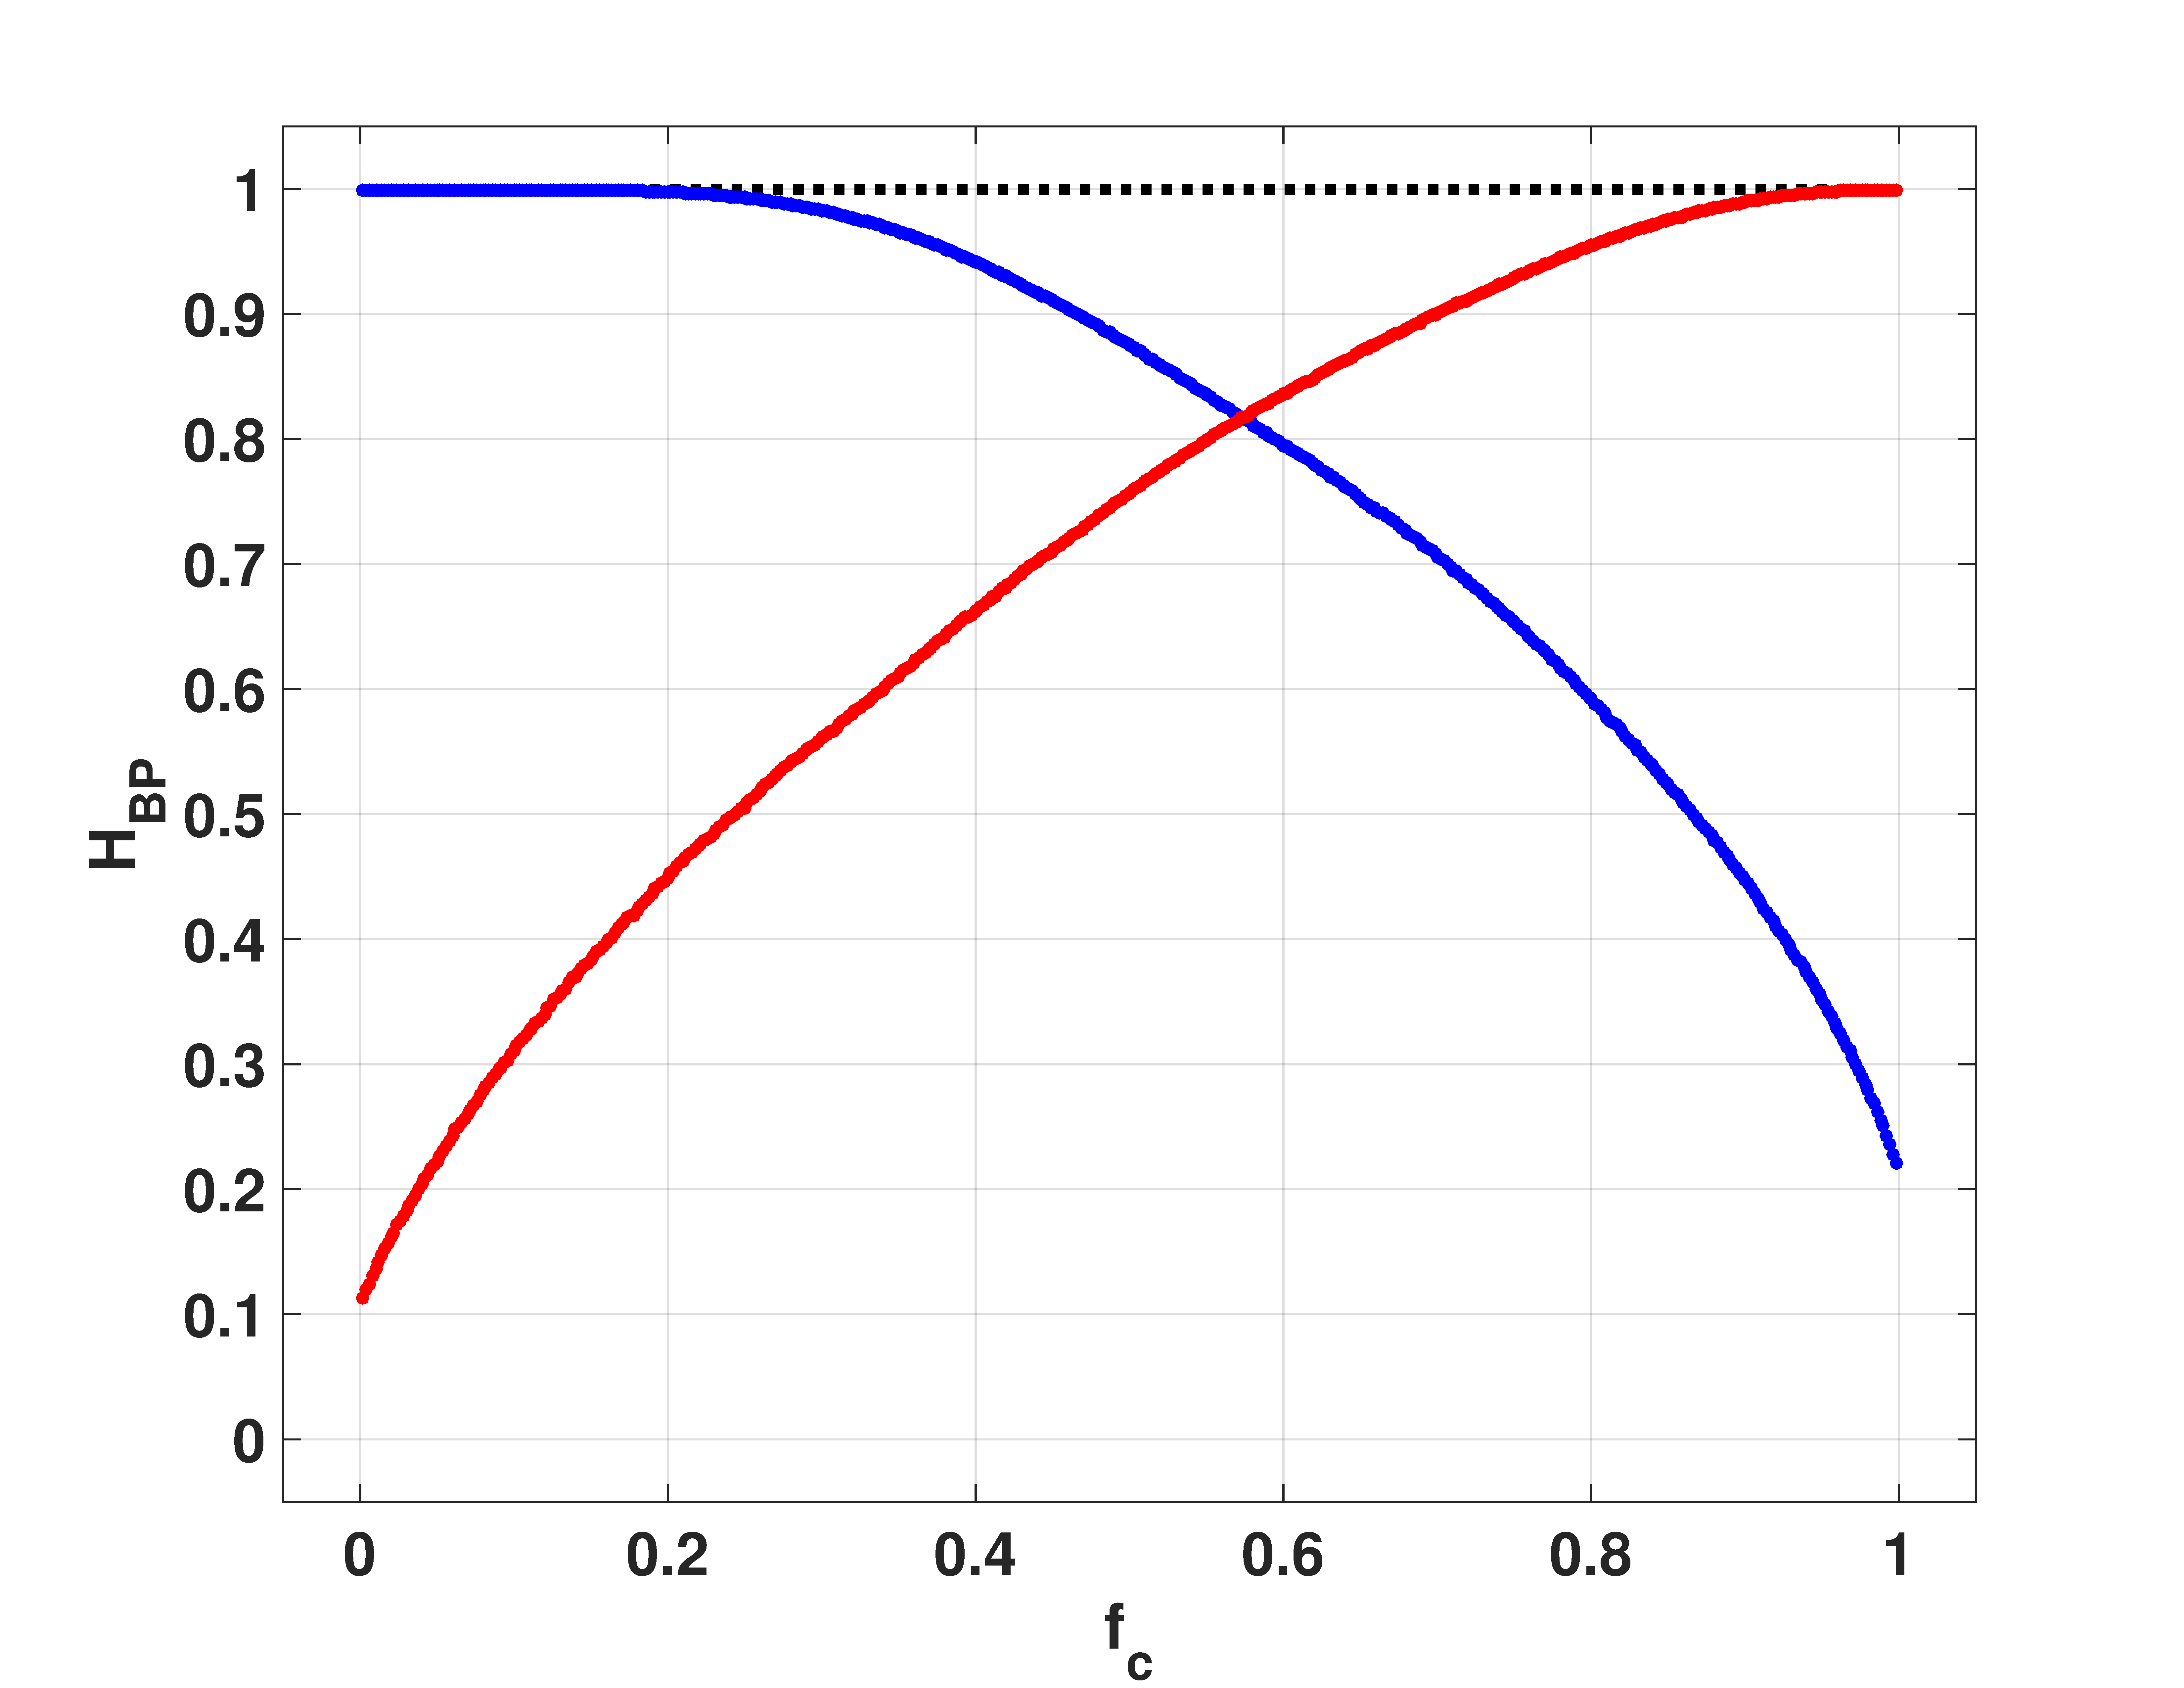
\includegraphics[width=\textwidth]{Ruido_Hbp}
        \caption{Entropía de patrones de orden normalizada}
        \label{subfig:ideal_Hbp}
    \end{subfigure}
    ~ %add desired spacing between images, e. g. ~, \quad, \qquad, \hfill etc. 
    %(or a blank line to force the subfigure onto a new line)
    \begin{subfigure}[t]{.49\textwidth}
        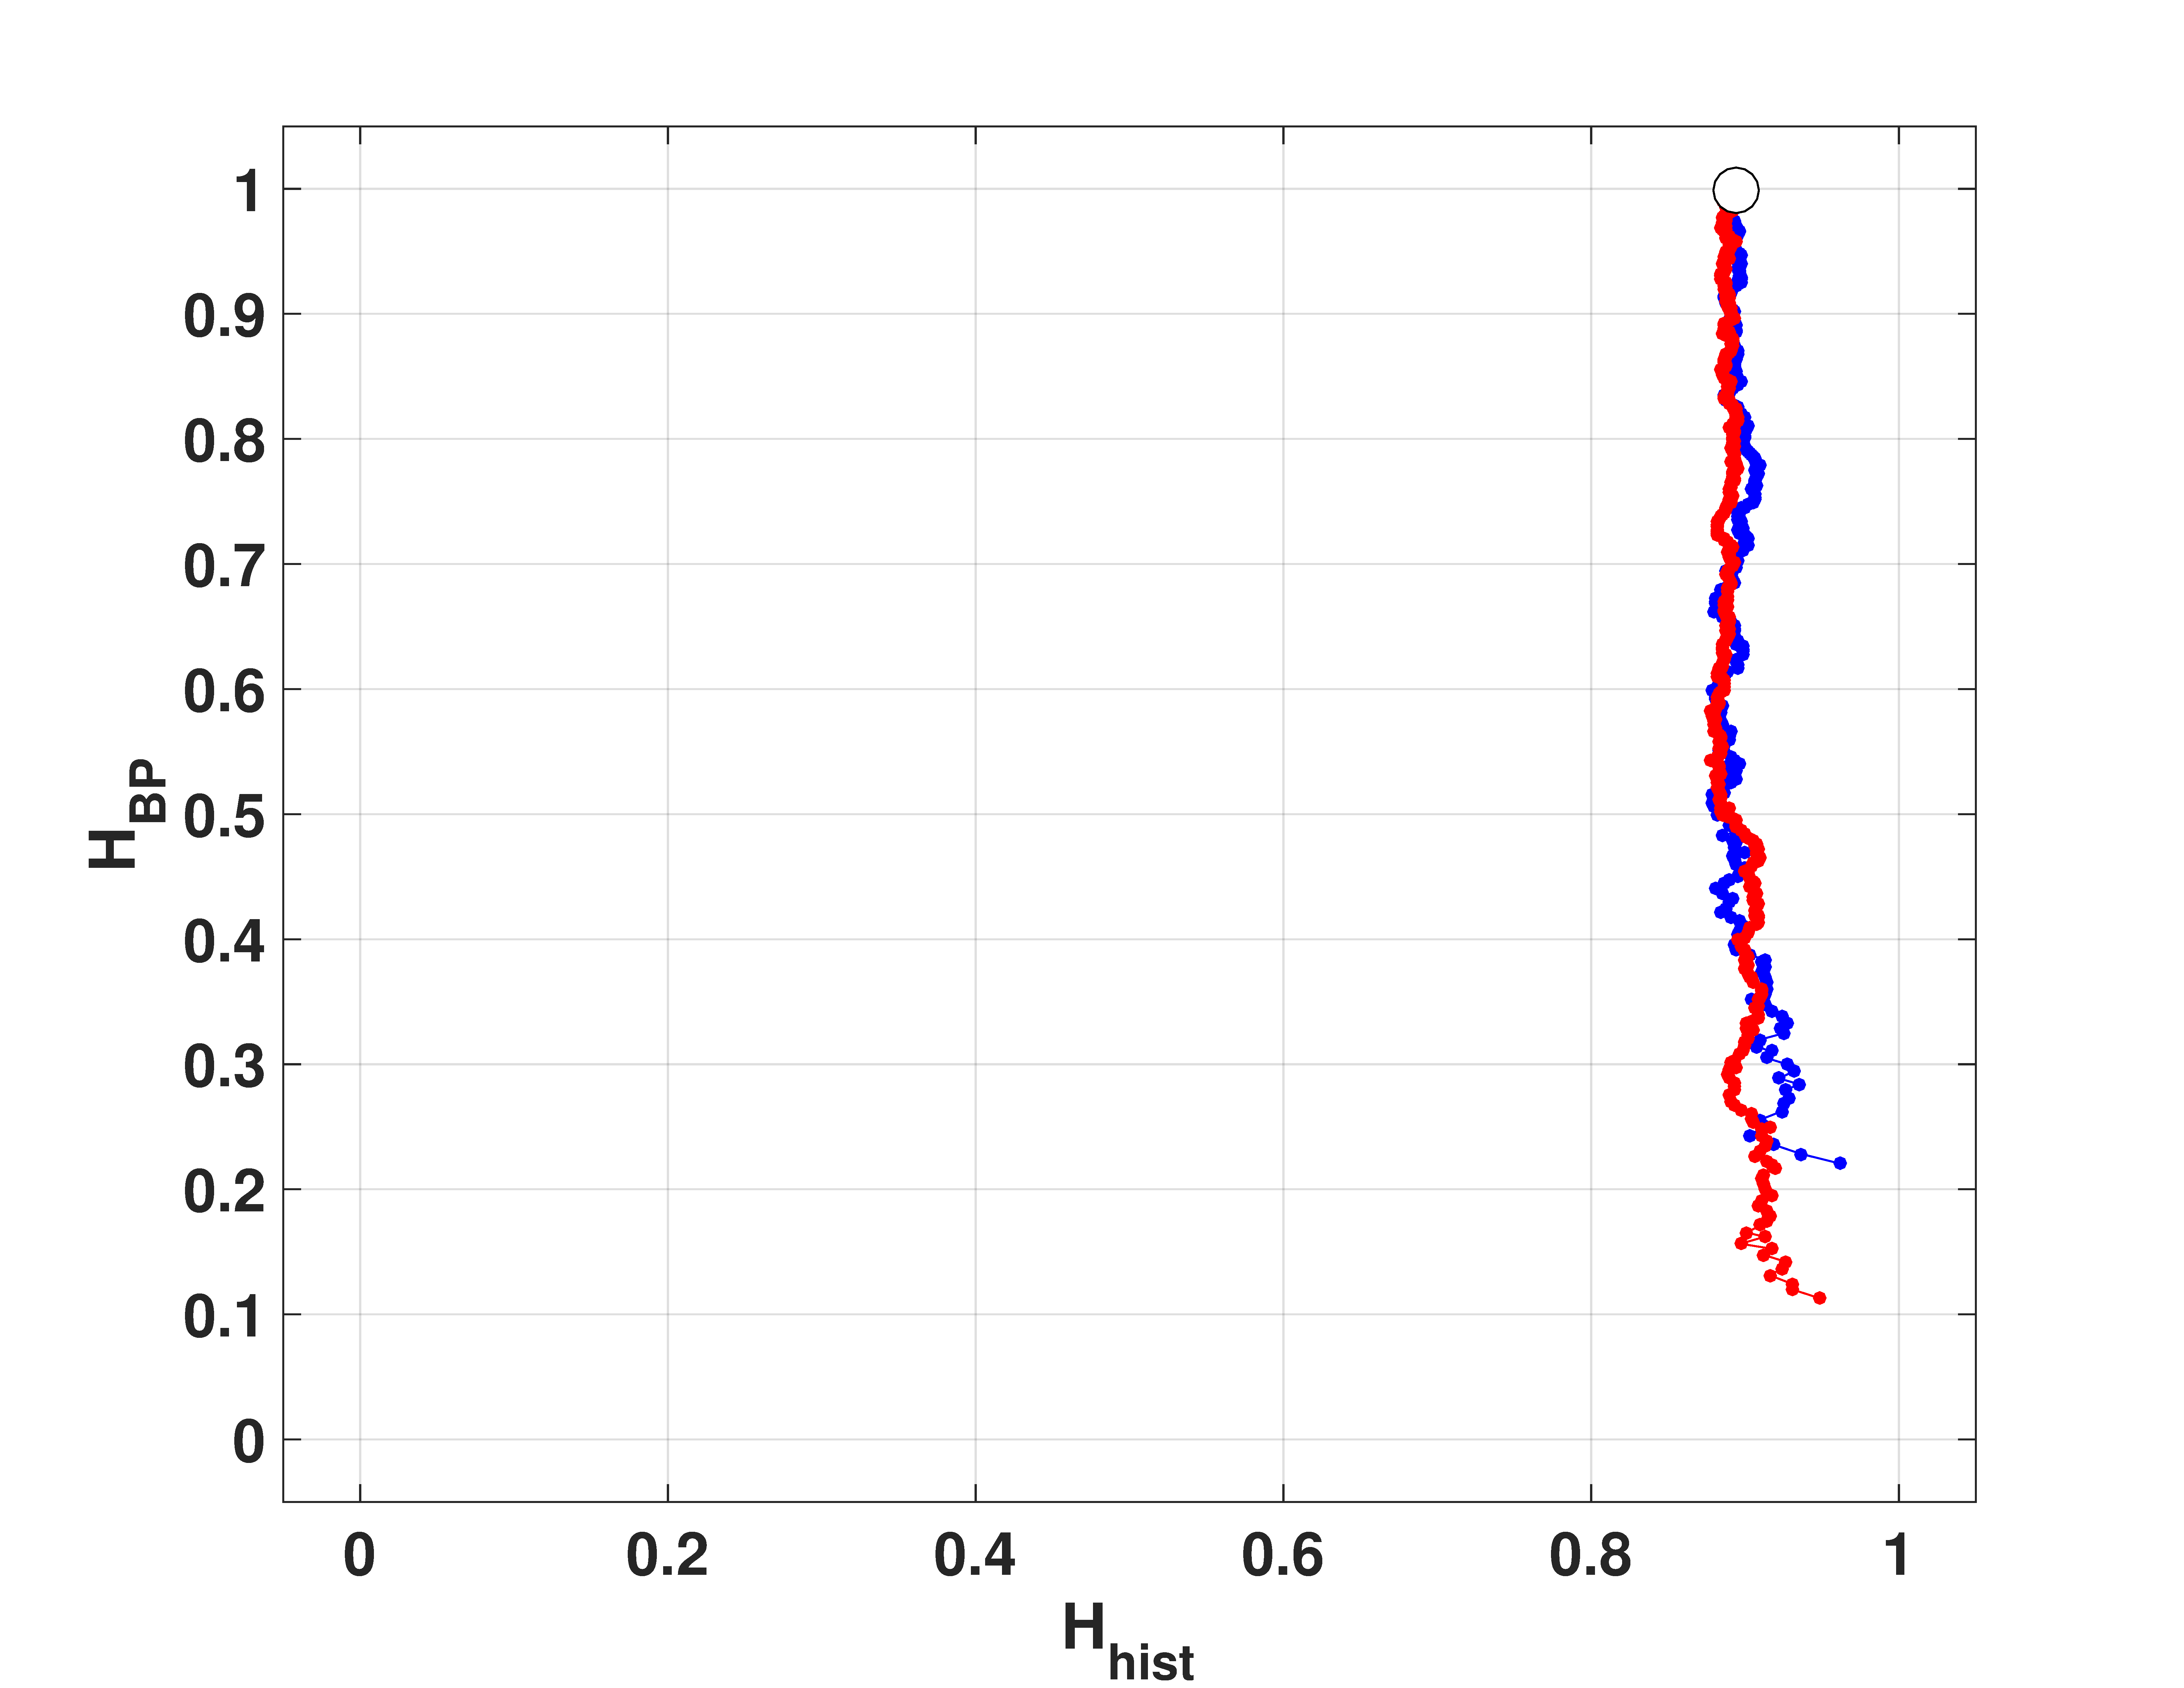
\includegraphics[width=\textwidth]{Ruido_Hbp_Hhist}
        \caption{Plano doble entropía}
        \label{subfig:ideal_HbpHhist}
    \end{subfigure}
    \caption{Cuantificadores calculados sobre la salida del filtro ideal cuando se ingresa con ruido blanco gaussiano.}\label{fig:ideal}
\end{figure}

Para el sistema planteado no se necesita volver al dominio continuo analógico, por lo que las dificultades mencionadas en la Sección \ref{sec:filtrado} respecto al filtrado ideal (como ripple en las bandas de paso y rechazo) no aplican a este caso.
Por este motivo para esta serie de pruebas elegimos el filtro ideal, dado que presenta mejores resultados que el elíptico.

La primer señal determinística que se muestra es una senoidal de amplitud unitaria con $100$ muestras por período, los resultados pueden verse en la Figura \ref{fig:Senoidal}.
Mientras la única componente espectral no es filtrada, el valor de la entropía de valores es $H_{hist}\approx0,57$ en la Figura \ref{subfig:Senoidal_Hhist} y la entropía de patrones de orden $H_{BP}\approx0,16$ en la Figura \ref{subfig:Senoidal_Hbp}.
Ambos cuantificadores caen a cero cuando la única componente espectral es filtrada, ya sea por el filtro pasa-bajos (azul) o por el pasa-altos (rojo).
El plano doble entropía muestra un punto en $\left(0,57;0,16\right)$ para la senoidal sin filtrar y otro en $\left(0;0\right)$ cuando la única componente espectral es filtrada.
%
\begin{figure}[h]
    \centering
    \begin{subfigure}[t]{.49\textwidth}
        \includegraphics[width=\textwidth]{Senoidal_Hhist}
        \caption{Entropía de valores normalizada}
        \label{subfig:Senoidal_Hhist}
    \end{subfigure}
    ~ %add desired spacing between images, e. g. ~, \quad, \qquad, \hfill etc. 
      %(or a blank line to force the subfigure onto a new line)
    \begin{subfigure}[t]{.49\textwidth}
        \includegraphics[width=\textwidth]{Senoidal_Hbp}
        \caption{Entropía de patrones de orden normalizada}
        \label{subfig:Senoidal_Hbp}
    \end{subfigure}
    ~ %add desired spacing between images, e. g. ~, \quad, \qquad, \hfill etc. 
    %(or a blank line to force the subfigure onto a new line)
    \begin{subfigure}[t]{.49\textwidth}
        \includegraphics[width=\textwidth]{Senoidal_Hbp_Hhist}
        \caption{Plano doble entropía}
        \label{subfig:Senoidal_HbpHhist}
    \end{subfigure}
    \caption{Cuantificadores calculados sobre la salida del filtro ideal cuando se ingresa con una señal senoidal limpia.}\label{fig:Senoidal}
\end{figure}

La salida de los cuantificadores cuando esta señal es contaminada con ruido gaussiano aditivo con $\sigma=0,2$ puede verse en la Figura \ref{fig:SenoidalRuidosa}.
Vemos en la Figura \ref{subfig:SenoidalRuidosa_Hhist} que la entropía de valores aumenta cuando el filtrado no elimina la componente espectral, dando valores incluso por encima del valor de la entropía de la señal gaussiana.
Esto se debe a que la PDF de amplitudes de la señal senoidal es complementaria con la de la señal gaussiana, entonces la PDF de amplitudes de la resultante es más parecida a la del ruido uniforme.
Para los patrones de orden de la Figura \ref{subfig:SenoidalRuidosa_Hbp}, el filtro pasa-altos no deja ver un cambio significativo debido a que la componente espectral de la senoidal es eliminada en la zona en la que su entropía es alta.
El filtro pasa-bajos en cambio muestra que mientras esta componente está presente el valor de la entropía es asintótico a el valor $H_{BP}\to0,16$ a medida que la frecuencia de corte disminuye.
Recordemos que $H_{BP}\approx0,16$ es el valor de la entropía de patrones de orden de la señal senoidal limpia.
En el plano doble entropía (Figura \ref{subfig:SenoidalRuidosa_HbpHhist}) se ve que ambos cuantificadores son complementarios, en el sentido que la entropía de valores detecta la presencia o no de la señal determinística mientras que la entropía de patrones de orden detecta el efecto del filtrado sobre la señal de ruido.
%
\begin{figure}[h]
    \centering
    \begin{subfigure}[t]{.49\textwidth}
        \includegraphics[width=\textwidth]{SenoidalRuidosa_Hhist}
        \caption{Entropía de valores normalizada}
        \label{subfig:SenoidalRuidosa_Hhist}
    \end{subfigure}
    ~ %add desired spacing between images, e. g. ~, \quad, \qquad, \hfill etc. 
      %(or a blank line to force the subfigure onto a new line)
    \begin{subfigure}[t]{.49\textwidth}
        \includegraphics[width=\textwidth]{SenoidalRuidosa_Hbp}
        \caption{Entropía de patrones de orden normalizada}
        \label{subfig:SenoidalRuidosa_Hbp}
    \end{subfigure}
    ~ %add desired spacing between images, e. g. ~, \quad, \qquad, \hfill etc. 
    %(or a blank line to force the subfigure onto a new line)
    \begin{subfigure}[t]{.49\textwidth}
        \includegraphics[width=\textwidth]{SenoidalRuidosa_Hbp_Hhist}
        \caption{Plano doble entropía}
        \label{subfig:SenoidalRuidosa_HbpHhist}
    \end{subfigure}
    \caption{Cuantificadores calculados sobre la salida del filtro ideal cuando se ingresa con una señal senoidal ruidosa.}\label{fig:SenoidalRuidosa}
\end{figure}

En la Figura \ref{fig:Cuadrada} se muestran los resultados cuando la señal determinística es una cuadrada de amplitud unitaria sin ruido y $100$ muestras por período.
Tanto la entropía de valores $H_{hist}$ como la entropía de patrones de orden $H_{BP}$ presentan una forma escalonada, sus valores se mantienen constantes a medida que se barre la frecuencia de corte de los filtros hasta que la siguiente componente espectral es filtrada.
También se ve que en ambos casos los valores resultantes se mantienen bastante lejos del valor sin filtrar, el cual es indicado con una linea negra punteada.
%
\begin{figure}[h]
    \centering
    \begin{subfigure}[t]{.49\textwidth}
        \includegraphics[width=\textwidth]{Cuadrada_Hhist}
        \caption{Entropía de valores normalizada}
        \label{subfig:Cuadrada_Hhist}
    \end{subfigure}
    ~ %add desired spacing between images, e. g. ~, \quad, \qquad, \hfill etc. 
      %(or a blank line to force the subfigure onto a new line)
    \begin{subfigure}[t]{.49\textwidth}
        \includegraphics[width=\textwidth]{Cuadrada_Hbp}
        \caption{Entropía de patrones de orden normalizada}
        \label{subfig:Cuadrada_Hbp}
    \end{subfigure}
    ~ %add desired spacing between images, e. g. ~, \quad, \qquad, \hfill etc. 
    %(or a blank line to force the subfigure onto a new line)
    \begin{subfigure}[t]{.49\textwidth}
        \includegraphics[width=\textwidth]{Cuadrada_Hbp_Hhist}
        \caption{Plano doble entropía}
        \label{subfig:Cuadrada_HbpHhist}
    \end{subfigure}
    \caption{Cuantificadores calculados sobre la salida del filtro ideal cuando se ingresa con una cuadrada limpia.}\label{fig:Cuadrada}
\end{figure}

El caso contaminado con ruido (Figura \ref{fig:CuadradaRuidosa}) cambia respecto del caso sin contaminar.
En la Figura \ref{subfig:CuadradaRuidosa_Hhist} se ve que para el filtro pasabajos (rojo) $H_{hist}$ se mantiene alrededor del valor sin filtrar (linea punteada), excepto con las tres frecuencias más bajas, en donde su valor aumenta un levemente por las mismas razones que aumentaba con la senoidal contaminada.
Algo parecido sucede con $H_{BP}$ en la Figura \ref{subfig:CuadradaRuidosa_Hbp}.
Cuando la señal cuadrada se contamina con ruido su valor se mantiene cercano al del ruido gaussiano, esto es por que en las regiones en las que la señal cuadrada es plana su contribución al patrón de orden es nula.
Para el filtro pasa bajos se ve un escalonado en la posición de cada componente espectral que se hace más notorio para las frecuencias más bajas, en donde la contribución del ruido ya es bastante baja y a la vez se encuentran las componentes espectrales de mayor peso.
Esto no es tan notorio en el filtro pasa-altos, en este caso cuando la contribución del ruido es de baja amplitud también lo es la de la señal determinística, enmascarando este fenómeno.
%
\begin{figure}[h]
    \centering
    \begin{subfigure}[t]{.49\textwidth}
        \includegraphics[width=\textwidth]{CuadradaRuidosa_Hhist}
        \caption{Entropía de valores normalizada}
        \label{subfig:CuadradaRuidosa_Hhist}
    \end{subfigure}
    ~ %add desired spacing between images, e. g. ~, \quad, \qquad, \hfill etc. 
      %(or a blank line to force the subfigure onto a new line)
    \begin{subfigure}[t]{.49\textwidth}
        \includegraphics[width=\textwidth]{CuadradaRuidosa_Hbp}
        \caption{Entropía de patrones de orden normalizada}
        \label{subfig:CuadradaRuidosa_Hbp}
    \end{subfigure}
    ~ %add desired spacing between images, e. g. ~, \quad, \qquad, \hfill etc. 
    %(or a blank line to force the subfigure onto a new line)
    \begin{subfigure}[t]{.49\textwidth}
        \includegraphics[width=\textwidth]{CuadradaRuidosa_Hbp_Hhist}
        \caption{Plano doble entropía}
        \label{subfig:CuadradaRuidosa_HbpHhist}
    \end{subfigure}
    \caption{Cuantificadores calculados sobre la salida del filtro ideal cuando se ingresa con una cuadrada ruidosa.}\label{fig:CuadradaRuidosa}
\end{figure}

Para caracterizar el comportamiento de los cuantificadores frente a la amplitud de ruido, se generaron señales cuadradas contaminadas con AWGN de dos amplitudes y se filtraron para calcular los cuantificadores.
En la Figura \ref{fig:HCuadradaRuidosa_Sigma} se muestran ambos cuantificadores cuando se hace variar el ruido con valores de la desviación estándar $\sigma=[0~0,1~1]$.
Cuando comparamos las Figuras \ref{subfig:HhistCuadradaRuidosa_Sigma_0}, \ref{subfig:HhistCuadradaRuidosa_Sigma_0p1} y \ref{subfig:HhistCuadradaRuidosa_Sigma_1} vemos un cambio significativo cuando pasamos de la señal limpia de \ref{subfig:HhistCuadradaRuidosa_Sigma_0} a la contaminada con bajos niveles de ruido de la \ref{subfig:HhistCuadradaRuidosa_Sigma_0p1}, sin embargo cuando pasamos del bajo nivel de ruido de la Figura \ref{subfig:HhistCuadradaRuidosa_Sigma_0p1} al de la Figura \ref{subfig:HhistCuadradaRuidosa_Sigma_1} el cambio es mucho más sutil.
De modo similar, entre las Figuras \ref{subfig:HbpCuadradaRuidosa_Sigma_0} y \ref{subfig:HbpCuadradaRuidosa_Sigma_0p1} hay muy pocas similitudes, mientras que las Figuras \ref{subfig:HbpCuadradaRuidosa_Sigma_0p1} y \ref{subfig:HbpCuadradaRuidosa_Sigma_1} son bastante similares.
En este segundo caso es más evidente la diferencia cuando cambia el nivel de ruido, con bajos niveles puede verse el escalonado que aparece cada vez que una frecuencia es filtrada, mientras que cuando la amplitud de ruido es mayor este escalonado aparece solo en el pasabajos para las tres primeras frecuencias, que resultan ser las de mayor peso.
%
\begin{figure}[h]
    \centering
    \begin{subfigure}[t]{.49\textwidth}
        \includegraphics[width=\textwidth]{Cuadrada_Hhist}
        \caption{$H_{hist}$ con $\sigma=0$}
        \label{subfig:HhistCuadradaRuidosa_Sigma_0}
    \end{subfigure}
    ~ %add desired spacing between images, e. g. ~, \quad, \qquad, \hfill etc. 
      %(or a blank line to force the subfigure onto a new line)
    \begin{subfigure}[t]{.49\textwidth}
        \includegraphics[width=\textwidth]{CuadradaRuidosa_Hhist_S0p1}
        \caption{$H_{hist}$ con $\sigma=0,1$}
        \label{subfig:HhistCuadradaRuidosa_Sigma_0p1}
    \end{subfigure}
    ~ %add desired spacing between images, e. g. ~, \quad, \qquad, \hfill etc. 
    %(or a blank line to force the subfigure onto a new line)
    \begin{subfigure}[t]{.49\textwidth}
        \includegraphics[width=\textwidth]{CuadradaRuidosa_Hhist_S1}
        \caption{$H_{hist}$ con $\sigma=1$}
        \label{subfig:HhistCuadradaRuidosa_Sigma_1}
    \end{subfigure}
    \begin{subfigure}[t]{.49\textwidth}
        \includegraphics[width=\textwidth]{Cuadrada_Hbp}
        \caption{$H_{BP}$ con $\sigma=0$}
        \label{subfig:HbpCuadradaRuidosa_Sigma_0}
    \end{subfigure}
    ~ %add desired spacing between images, e. g. ~, \quad, \qquad, \hfill etc. 
      %(or a blank line to force the subfigure onto a new line)
    \begin{subfigure}[t]{.49\textwidth}
        \includegraphics[width=\textwidth]{CuadradaRuidosa_Hbp_S0p1}
        \caption{$H_{BP}$ con $\sigma=0,1$}
        \label{subfig:HbpCuadradaRuidosa_Sigma_0p1}
    \end{subfigure}
    ~ %add desired spacing between images, e. g. ~, \quad, \qquad, \hfill etc. 
    %(or a blank line to force the subfigure onto a new line)
    \begin{subfigure}[t]{.49\textwidth}
        \includegraphics[width=\textwidth]{CuadradaRuidosa_Hbp_S1}
        \caption{$H_{BP}$ con $\sigma=1$}
        \label{subfig:HbpCuadradaRuidosa_Sigma_1}
    \end{subfigure}
    \caption{Cuantificadores calculados sobre la salida del filtro ideal cuando se ingresa con cuadradas contaminadas con AWGN con amplitudes de ruido $\sigma=[0~0.1~1]$.}\label{fig:HCuadradaRuidosa_Sigma}
\end{figure}
\thispagestyle{empty}

\chapter{El problema de la Aritmética Discreta}

\section{Analysis of the digital implementation of a chaotic deterministic-stochastic attractor (EAMTA 2012)}

Otro que no tengo el latex, se lo tengo que pedir a Luciana

In this work the implementation, of chaos-based
pseudo random number generators (PRNG), onto a Field Programmable Gate Array (FPGA), is analyzed. Any digital implementation requires the choice of an algorithm to discretize
time and a representation standard to represent real numbers.
Each choice modifies the stochasticity degree of the system and
also defines a different amount of resources on the FPGA. The
main contribution of this paper is to propose an optimum design
methodology for applications in which the chaotic system is going
to replace a stochastic system. This is the case with PRNG. In
stochastic systems the randomness degree must be measured. In
this paper we use the global indicator proposed by Marsaglia
in his widely used DIEHARD tests-suite. Results are exemplified
for the Lorenz chaotic oscillator but the same methodology may
be used with other low dimensional chaotic systems.

%%%%%%%%%%%%%%%%%%%%%%%%%%%%%%%%%%%%%%%%%%%%%%%%%%%%%%%%%%%%%%%%%%%%%%%%%%%%%%%%%%%%%%%%%%%%%%%%%%%%%%%%%%%%%%%%
\section{Complexity of switching chaotic maps}

\subsection{Introduction}
In the last years digital measuring systems become the standard in
all experimental sciences. By using \emph{virtual instruments} and new programable electronic
devices, such as Digital Signal Processors ($DSP$) and Field
Programmable Gate Arrays ($FPGA$)  experimenters may design and
modify their own measuring systems.

The effect of finite precision in these new devices needs to be
investigated. This issue is critical if  chaotic systems must be implemented, because due to roundoff errors digital implementations will always become periodic with a period $T$ and unstable orbits with a low period may become stable destroying completely the chaotic behavior.  
Grebogi and coworkers \cite{Grebogi1988} studied this subject and they shaw that the period $T$ scales with roundoff $\epsilon$ as
$T\sim\epsilon^{-d/2}$ where $d$ is the correlation dimension of
the chaotic attractor. 

To have a large period $T$ is one an important property of a chaotic map. Stochasticity and mixing are also relevant. Furthermore to characterize these properties several quantifiers were
studied  \cite{DeMicco2009}. Among them the use of an
entropy-complexity representation ($H-C$ plane) deserves special
consideration\cite{Rosso2007C,DeMicco2008,DeMicco2011,DeMicco2009,Rosso2009}. 
A fundamental issue is the criterium to select the distribution function ($PDF$) assigned to the time series. Causal and non causal options are possible. Here we consider the non-causal traditional $PDF$ obtained by normalization of the histogram of the time series. Its statistical quantifier is the normalized entropy$H_{hist}$ that is  a measure of equiprobability among all allowed values. We also consider a causal $PDF$  that is obtained by assigning ordering patterns to segments of trajectory of length $D$. This PDF were first proposed by Bandt \& Pompe in a seminal paper \cite{Pompe2002}. The corresponding entropy $H_{BP}$ was also proposed as a quantifier by Bandt \& Pompe. Amig\'o and coworkers proposed the number of forbidden patterns as a quantifier of chaos \cite{Amigo2007b}. Essentialy they reported the presence of forbidden patterns as an indicator of chaos. Recently it was shown that the name forbidden patterns is not convenient and it was replaced by  \emph{missing patterns}(MP) \cite{Rosso2012b}. 

Switching systems naturally arise in power electronics and many other areas in digital electronics. They have also interest in transport problems in deterministic ratchets \cite{Zarlenga2009} and it is known that synchronization of the switching procedure affects the output of the controlled system. Nagaraj et al \cite{Nagaraj2008} studied the case of switching between two maps. They shaw that the period $T$ of the
compound map obtained by switching between two chaotic maps is
higher than the period of each map.  Liu et al \cite{Liu2006} studied different switching rules applied to linear systems to generate chaos. Switching chaos was also addressed in \cite{Gluskin2008}.  Skipping values of the time series is another simple technique used to increase mixing in chaotic maps \cite{DeMicco2008}. 

In this paper we study the statistical characteristic of two well known maps: the tent map (TENT) and logistic map (LOG). Three additional maps are generated: 1) SWITCH, generated by switching between TENT and LOG; 2) EVEN, generated by skipping all the elements in odd position in SWITCH time series and 3) ODD, generated by discarding all the elements in an even position in SWITCH time series. Floating point, decimal numbers and binary numbers are used. All these specific numerical systems may be implemented in modern programmable logic boards. 

The main contributions of this paper are:
\begin{enumerate}
\item the definition of different statistical quantifiers and their relationship  with the properties of the time series generated by the map. 
\item the study of how this quantifiers are modified by the numerical representation using floating point, decimal and binary numbers. It is specially interesting to note that some systems (TENT) with very nice statistical properties in the world of the real numbers, become ``pathological" when numerical representations are used.
\item the effect of switching between two different maps, on the period and the statistical properties of the time series. Floating point, decimal and binary numerical representations are considered. 
\item the effect of skipping values in any of these maps
\end{enumerate}

Organization of the paper is as follows: section \ref{sec:quanti} describes the statistical quantifiers used in the paper and the relationship between their value and characteristics of the causal and non causal PDF considered; section \ref{sec:resultados} shows and discuss the results obtained for all the numerical representations. Finally section  \ref{sec:conclusions} deals with final remarks and future work. 
%
\subsection{Information theory quantifiers}\label{sec:quant}
The first step to quantify the statistical properties of the values (amplitude statistics) of a time series $\{x_i,~(i=1,...,N)\}$, using information theory is to determine the concomitant PDF because all the quantifiers are functionals of the PDF associated to the time series. This is an issue studied in detail in previous papers \cite{aka varios}. Let us summarize the procedure:
\begin{enumerate} 
\item \label{1} a finite alphabet  with $M$ symbols $\mathbf{ A}=\{a_1,...,a_M\}$ is chosen. 
\item \label{2} one of these symbols is assigned: (a) to each value of the time series of (b) to each portion of length $D$ of the trajectory. 
\item \label{3} the normalized histogram of the symbols is the desired $PDF$.
\end{enumerate}

Note that if option (a) is chosen in step \ref{2} then the PDF is \emph{non causal}, because all the information about the time evolution of the system generating $\{x_i\}$  is completely lost. On the contrary if option (b) is chosen in step \ref{2} then the PDF is \emph{causal}, in the sense it has some information about the temporal evolution.

 Of course there are infinite possibilities to choose the alphabet $\mathbf{ A}$ as well as the length $D$.
Bandt \& Pompe made a proposal for a causal PDF that has been shown to be easy to implement and useful in a great variety of applications.  The procedure is the
following \cite{Pompe2002,Keller2003,Keller2005}:
\begin{itemize}
\item Given a
series $\{x_t : t=0, \Delta t, \cdots,M\Delta t \}$, a sequence of
vectors of length $d$ is generated.

\begin{equation}
\label{eq:vectores}
(s)\mapsto \left(x_{t-(d-1)\Delta t},x_{t-(d-2)\Delta t},\cdots,x_{t-\Delta t},x_{t}\right) \ ,
\end{equation}

Each vector turns out to be the ``history'' of the value $x_t$.
Clearly, the longer the length of the vectors $D$, the more
information about the history would the vectors have but a higher value of $N$ is required to have an adequate statistics. 
\item The
permutations $\pi=(r_0, r_1, \cdots, r_{D-1})$ of $(0, 1, \cdots,
D-1)$ are called ``order of patterns'' of time $t$, defined by:

\begin{equation}
\label{eq:permuta}
x_{t-r_{D-1}\Delta t}\le x_{t-r_{D-2}\Delta t}\le\cdots\le x_{t-r_{1}\Delta t}\le x_{t-r_0\Delta t}.
\end{equation}
%
In order to obtain an unique result it is considered $r_i
<r_{i-1}$ if $x_{t-r_{i}\Delta t}=x_{t-r_{i-1}\Delta t}$.

In this way, all the $D!$ possible permutations $\pi$ of order
$D$, and the PDF $P=\{p(\pi)\}$ is defined as:

\begin{equation}
\label{eq:frequ}
p(\pi)~=~ \frac{\sharp \{s|s\leq M-D+1; (s) \quad \texttt{has type}~\pi\}}{M-D+1}.
\end{equation}
In the last expression the $\sharp$ symbol means ``number".
\end{itemize}
This procedure has the advantages of being {\it i)\/} simple, {\it
ii)\/} fast to calculate, {\it iii)\/} robust in presence of
noise, and {\it iv)\/} invariant to lineal monotonous
transformations.

It is applicable to weak stationarity processes (for
$k=D$, the probability that $x_t < x_{t+k}$ doesn't depend on the
particulary $t$ \cite{Pompe2002}).The causality property of the
PDF allows the quantifiers (based on this PDFs) to discriminate
between deterministic and stochastic systems \cite{Rosso2007B}.

According to this point Bandt and Pompe suggested $3\leq D \leq
7$. $D=6$ has been adopted in this work.

Based on our previous research \cite{DeMicco2008,DeMicco2009} we have employed two $PDF$'s: (a) the normalized histogram of the time series amplitudes $\{x_i\}$ (that is a non-causal $PDF$), and (b) the Bandt \& Pompe $PDF$ (that is a causal $PDF$).
The entropies $H_{hist}$ and $H_{BP}$, the statistical complexity $C_{BP}$  are used as quantifiers.  

We also used the number of missing patterns $MP$ as a quantifier\cite{Rosso2012}. As shown recently by Amig\'o {\it et al.\/}
\cite{Amigo2006,Amigo2007,Amigo2008,Amigo2010},  in the case of
deterministic one-dimensional maps, not all the possible ordinal patterns
can be effectively materialized into orbits, which in a sense
makes these patterns ``forbidden". Indeed, the existence of these
{\it forbidden ordinal patterns\/} becomes a persistent fact that
can be regarded as a ``new" dynamical property. Thus, for a fixed
pattern-length (embedding dimension $D$) the number of forbidden
patterns of a time series (unobserved patterns) is independent of
the series length $N$. Remark that this independence does not
characterize other properties of the series such as proximity and
correlation, which die out with time \cite{Amigo2007,Amigo2010}.

A full discussion about the convenience of using these quantifiers is
out of the scope of this work. Nevertheless reliable bibliographic
sources do exist
\cite{Wackerbauer1994,Lopez1995,Rosso2007A,DeMicco2008,Rosso2009,Martin2006,Rosso2012}.

The entropies $H_{hist}$ and $H_{BP}$ are the normalized version of the  Of course there are infinite possibilities to choose the alphabet as well as the length $d$.
Bandt \& Pompe made a proposal for a causal PDF that has been shown to be easy to implement and useful in a great variety of applications.  The procedure is the
following \cite{Pompe2002,Keller2003,Keller2005}: a) Given a
series $\{x_t : t=0, \Delta t, \cdots,M\Delta t \}$, a sequence of
vectors of length $d$ is generated.

\begin{equation}
\label{eq:vectores}
(s)\mapsto \left(x_{t-(d-1)\Delta t},x_{t-(d-2)\Delta t},\cdots,x_{t-\Delta t},x_{t}\right) \ ,
\end{equation}

Each vector turns out to be the ``history'' of the value $x_t$.
Clearly, the longer the length of the vectors $d$, the more
information about the history would the vectors have. b) The
permutations $\pi=(r_0, r_1, \cdots, r_{d-1})$ of $(0, 1, \cdots,
d-1)$ are called ``order of patterns'' of time $t$, defined by:

\begin{equation}
\label{eq:permuta}
x_{t-r_{d-1}\Delta t}\le x_{t-r_{d-2}\Delta t}\le\cdots\le x_{t-r_{1}\Delta t}\le x_{t-r_0\Delta t}.
\end{equation}
%
In order to obtain an unique result it is considered $r_i
<r_{i-1}$ if $x_{t-r_{i}\Delta t}=x_{t-r_{i-1}\Delta t}$.

In this way, all the $d!$ possible permutations $\pi$ of order
$d$, and the PDF $P=\{p(\pi)\}$ is defined as:

\begin{equation}
\label{eq:frequ}
p(\pi)~=~ \frac{\sharp \{s|s\leq M-Dd+1; (s) \quad \texttt{has type}~\pi\}}{M-d+1}.
\end{equation}
In the last expression the $\sharp$ symbol means ``number".

This procedure has the advantages of being {\it i)\/} simple, {\it
ii)\/} fast to calculate, {\it iii)\/} robust in presence of
noise, and {\it iv)\/} invariant to lineal monotonous
transformations.

It is applicable to weak stationarity processes (for
$k=d$, the probability that $x_t < x_{t+k}$ doesn't depend on the
particulary $t$ \cite{Pompe2002}).The causality property of the
PDF allows the quantifiers (based on this PDFs) to discriminate
between deterministic and stochastic systems \cite{Rosso2007B}.

The choice of the embedding dimension $d$ is crucial because it
determines the minimal length acceptable of the original temporal
series ($M \gg d!$) needed to obtain an adequate statistics.
According to this point Bandt and Pompe suggested $3\leq d \leq
7$. $d=6$ has been adopted in this work.

Based on our previous research \cite{DeMicco2009} we have employed
the statistical complexity $C$ and the entropy $H$ to define a plane where the stochasticiy of the chaotic system may be represented. A full discussion about the convenience of using these quantifiers is
out of the scope of this work. Nevertheless reliable bibliographic
sources do exist
\cite{Wackerbauer1994,Lopez1995,Rosso2007A,DeMicco2008,Rosso2009,Martin2006}.

The entropy $H[P]$ is the normalized version of the Entropy proposed by Shannon \cite{Shannon1949a}:
\begin{equation}\label{eq:sha}
H[P] = S[P] /S_{max},
\end{equation}
where $S[P]=-\sum _{j=1}^{M}~p_j~\ln( p_j )$\\ and $S_{max}$ is
the normalizing constant:
\begin{equation}
\label{eq:Smax} S_{max}= S[P_e] = \ln M,
\end{equation}
and $P_e=\{ 1/M, \cdots,1/M\}$ is the uniform distribution. The number of symbols $M$ is equal to $N$ for $H_{hist}$ and it is equal to $D!$ for $H_{BP}$.

The statistical complexity $C[P]$ is given by:
\begin{equation}
\label{eq:inten}
C[{P}]=Q_{J}[{P,P_e}]\cdot H[{P}] \ ,
\end{equation}
, and
$Q_{J}$ is named ``disequilibrium'' and it is the distance between $P$ and $P_e$ 
 in the probability space. The metric used in this paper is based on the Jensen-Shannon divergence
 \cite{Lamberti2004}:
\begin{equation}
\label{eq:disequi}
Q_{J}[{P,P_e}]= Q_0 \cdot \{S[\frac{P+P_e}{2}]-S[P]/2-S[P_e]/2 \} \ .
\end{equation}
The normalization constant $Q_0$ is:
\begin{equation}
\label{eq:q0j}
Q_0=-2 \left\{ \left( \frac{N+1}{N} \right) \ln(N+1) - 2 \ln(2N) + \ln N \right\}^{-1} .
\end{equation}

From the statistical point of view the disequilibrium $Q_J$ is an
intensive magnitude, and it is $0$ if and only if $P=P_e$. It has
been proved that the $C[P]$ quantifies the presence of nonlinear
correlations typical of chaotic systems
\cite{Martin2003,Lamberti2004}. The complexity $C[P]$ is
independent from the entropy $H[P]$, as far as different $P$'s share
the same entropy $H[P]$ but they have different  complexity
$C[P]$.

Two representation planes are considered: $H_{BP}$ vs $H_{hist}$ \cite{DeMicco2008} and $H_{BP}$ vs $C_{BP}$ \cite{Rosso2007C}. In the first plane a higher value in any of the entropies,  $H_{BP}$ and $H_{hist}$, implies an increase in the uniformity of the involved $PDF$. The point $(1,1)$ represents the ideal case with uniform histogram and uniform distribution of ordering patterns.  In the second plane not the entire region $0<H_{BP}<1$, $0<C_{BP}<1$ is achievable. In fact for any $PDF$ the pairs $(H,C)$ of possible values fall between two extreme curves in the plane $H$-$C$ \cite{Anteneodo1996}. Fig. \ref{fig:planezone} shows two regions labeled as \emph{deterministic} and \emph{stochastic}. In fact transition from one region to the other are smooth and the division is a bit arbitrary. A more detailed discussion can be seen in \cite{Rosso2007C}. Ideal random systems having uniform Bandt \& Pompe $PDF$, are represented by the point $(1,0)$ \cite{Gonzalez2005} and a delta-like $PDF$ corresponds with the point $(0,0)$. 


%
\subsection{Results}\label{sec:resultados}
Five pseudo chaotic maps were studied. For each one a floating point representation, a decimal numbers representation with $1\leq P \leq 27$ and a binary numbers representation with $1\leq B \leq 27$ are considered. For each representation $1000$ time series were generated using randomly chosen initial conditions within the interval $[0,1]$. 
The studied maps are tent (TENT), logistic (LOG) a sequential switching between TENT and LOG (SWITCH). Furthermore a skipping randomization procedure is applied to SWITCH \cite{DeMicco2008}, discarding the values in the odd positions (EVEN) or the values in the even positions (ODD) respectively. Let us detail our results for each of these maps. 
\subsection {Simple maps.}\label{subsec:simples}
Here we report our results for both maps:
\begin{enumerate}
%
\item Tent map (TENT)
\begin{equation}\label{eq:tentmap}
x_{n+1}~=~ \left\{ \begin{array}{ll}
2~{x_n} & \textrm{if ~$0\leq x_n\leq 1/2$}\\
2~(1-{x_n}) & \textrm{if ~$1/2<x_n\leq 1$} 
\end{array} \right.  \ ,
\end{equation}
with $x_n\in\mathcal{R}$.
%
The Tent map has been extensively studied in the literature because theoretically it has nice  statistical properties that can be analytically obtained. For example it is easy to proof that it has a uniform histogram and consequently an ideal $H_{hist}=1$. The Perron-Frobenius operator and its corresponding eigenvalues and eigenfunctions may be also be analytically obtained for this map \cite{tent}. 

When this map is implemented in a computer using any numerical representation system (even floating point!) truncation errors rapidly increases and makes the unstable fixed point in $x^*=0$ becomes stable producing a short transitory followed by an infinite number of  $0$'s\cite{Jessa1993,Callegari1997}. Some authors \cite{buscar} have proposed to add a random perturbation to avoid this drawback of the Tent map. But this procedure introduces statistical properties of the random perturbation that are mixed with those of the Tent map itself.

Here we study the Tent map ``as it is«« without any artifact to evaluate its real instead of theoretical statistical properties. Note that to effectively work in a given representation it is necessary to change the expression of the map in order to make all the operations in the chosen representation numbers. For example, in the case of TENT the expression in decimal numbers is:

\begin{equation}\label{eq:tentdecbin}
x_{n+1}~=~ \left\{ \begin{array}{ll}
2~{x_n} & \textrm{if $0\leq x_n\leq 1/2$}\\
\epsilon \times floor\{\frac{2~-~2~x_n}{\epsilon}\} & \textrm{if $1/2<x_n\leq 1$} 
\end{array} \right.  \ ,
\end{equation}
with $\epsilon=10^{-P}$ for decimal numbers and $\epsilon=2^{-B}$ for binary numbers. In Eq. \ref{eq:tentdecbin} $x_n$ is either a decimal number with $P$ digits or a binary number with $B$ bits.

Figs. \ref{fig:tent} (a) to (e) show the different quantifiers for floating point and decimal numerical representation. In each figure from (a) to (c) a dashed line shows the value for the floating point representation. In figures (d) and (e) the star corresponds to the floating point case. In decimal representations the value of $H_{hist}$ remains almost constant for $11\leq P\leq 16$ (see Fig. \ref{fig:tent} (a)). Its value is $<H_{hist}>=0.8740$ with a variance $\sigma_{Hhist}=2.5 \times 10^{_6}$. For lower or higher values pf $P$ entropy decreases. This effect is due precisely to the stabilization of the fixed point at $x=0$. For ordering patterns entropy $H_{BP}$ an almost constant value is obtained for $8\leq P \leq 15$. The value is  $H_{BP}\simeq 0.6287$ with variance $\sigma_{H_{BP}}=4.8 \times 10^{-6}$ (see Fig. \ref{fig:tent} (b)). This rather small maximum value may be understood by seeing  Fig. \ref{fig:tent} (c), where the number of MP.
% 
is minimal for $P$ within the same range but it is still large: $645$ patterns are missing and only $75$ ordering patterns are present in the time series. Then, even with a uniform distribution between these $75$ patterns, entropy can not be higher than $ln(75)/ln(720)\simeq 0.65$. 
A more complete perspective of the statistical properties is obtained in Fig. \ref{fig:tent} (d) showing the representative point in the $H_{hist},H_{BP}$ plane for different precisions. Note that the best choice for maximum stochasticity is obtained for $11\leq P \leq 15$, with maximum attainable values for both entropies.
Increasing the number of decimal figures makes Tent map worst in the sense the system approaches the state for the floating point representation (the star at $(0,0)$. 
Statistical complexity $C_{BP}$ is also maximal for $8\leq P \leq 15$. 
Fig. \ref{fig:tent} (e) shows the representation on the $H_{BP},C_{BP}$ plane. In this plane it is also clear that the more stochastic option corresponds with  $11\leq P \leq 15$ but even in the optimum case the representative point is located in a position very similar to other chaotic maps, very far from the ideal point for stochastic systems in this plane that is $(1,0)$ \cite{Rosso2007C}.
Binary numerical representation of the Tent map remains very near to the floating point values for  $1 \leq B \leq 27 $ (see Fig. \ref{fig:tent} (f)).
The conclusion is it is convenient to use a decimal numbers representation with  $P=11$ to get the optimum time series for the Tent map. A higher number of decimal figures does not improve the statistical properties of the time series. Furthermore binary and floating point representations are not allowed. 
%
\item Logistic map (LOG)
Logistic map is representative of the very large family of quadratic maps. 
\begin{equation}\label{eq:logimap}
 x_{n+1}~=~4~x_n~(1-x_n) \ ,
\end{equation}
with $x_n\in\mathcal{R}$.
%
Figs. \ref{fig:LOGdecimal} (a) to (f) show the statistical properties of LOG map in floating point and decimal numbers representation. This map does not show the anomalies pointed above for the tent map. For $P\geq 10$ the values of $H_{hist}$, $H_{BP}$ and $C_{BP}$ remains almost identical to the values for the floating point representation. Their values are: $<H_{hist}>=0.8621$ with variance $\sigma_{H_{hist}}=0.062 \times 10^{-6}$; $<H_{BP}>=0.6292$ with variance $\sigma_{H_{BP}}=0.060 \times 10^{-6}$; $<C_{BP}>=0.4842$ with variance $\sigma_{C_{BP}}=0.0195 \times 10^{-6}$. Missing patterns stabilize in $645$ for $P \geq 8$ making $H_{BP}$ to rise to its floating point value $<H_{BP}>=0.629$ with variance $\sigma_{H_{BP}}=0.060 \times 10^{-8}$. Note again that the stable value of mission patters missing patterns $645$ makes the optimum $H_{BP} \leq ln(75)/ln(720) \simeq 0.65$. Then $P=10$ is the most convenient choice because an increase in the number of decimal figures does not improve the statistical properties. 
Figs. \ref{fig:LOGbin} show the corresponding figures for binary representations. The histogram entropy $H_{hist}$ does not reach its floating point value within the maximum number of bits used. In the case of missing patterns the stable number $645$ is obtained with $B \geq 25$. It means that using $B=25$ one obtains a time series with good statistical properties regarding the missing patterns, but distribution among the allowed binary values is not as uniform as can be obtained with a higher value of $B$. 
\end{enumerate}

In summary, a comparison between LOG and TENT maps shows that, in the case of decimal representation, the best choice for TENT ($P=11$) produces a higher value for $H_{hist}$ than the best choice for LOG ($P=10$). Ordering patterns and the statistical properties related to them, are almost identical for the optimum choices in both maps. In the case of binary numbers  only LOG  can be used because TENT is highly anomalous. 

\subsubsection{Sequential switching}
\begin{enumerate}
\item Sequential switching between Tent and Logistic maps (SWITCH)
SWITCH may be expressed as a composition between $M_1 \circ M_2$ given by the following recurrence:
%
\[ \left\{ \begin{array}{ccc}\label{eq:seq}
x_{n+2}~=~ 4~x_{n+1}~(1-{n+1}) \\
x_{n+1}~=~ \left\{ \begin{array}{ll}
2~{x_n} & \textrm{if $0\leq x_n\leq 1/2$}\\
2~(1-{x_n}) & \textrm{if $1/2<x_n\leq 1$} 
\end{array} \right.  \end{array}\right. \] 
with $x_n\in\mathcal{R}$.
%
Results with sequential switching are shown in Figs. \ref{fig:seqdec} (a) to (f) for decimal numbers. The floating point entropy value is $H_{hist}=0.8658$, a value very similar to the one obtained for the TENT map and higher to that obtained for LOG. For decimal numbers this value is reached for $12 \leq P \leq 27$. It means it is enough to use $12$ decimal figures to get the same distribution of values in the time series. Regarding ordering patterns the number of MP decreases to $586$, a value lower lower than the one obtained for any of two simple maps TENT and LOG. It means the entropy $H_{BP}$ may increase up to $ln(134)/ln(720)\simeq 0.74$ With decimal numbers the entropy $H_{BP} $stabilizes at $P=9$ with $<H_{BP}>\simeq 0.657$ and variance $\sigma_{H_{BP}} \simeq 0.13 \times 10^{-7}$. Note that the entropies $H_{hist}$ and $H_{BP}$ are not monotonously increasing with $P$.  Considering all the quantifiers $P=12$ is the minimum number of decimal figures and statistical characteristics of this combined map are better than those for each individual map.
%
Results with sequential switching in binary numbers are shown in Figs. \ref{fig:seqbin}. Results for a number of bits $B\simeq27$ are equivalent to those obtained for $P\simeq 9$ for decimal numbers. It means both representation are valid and equivalent in the sense they will require similar hardware resources. 
\item 
Skipping is a usual randomizing technique that increases the mixing quality of a single map and correspondingly increases the value of $H_{BP}$ and decreases $C_{BP} $ of the time series. Skipping does not change the values of $H_{hist}$ and $C_{hist}$ evaluated using the non causal PDF (normalized histogram)\cite{DeMicco2008}. In the case under consideration we study Even and Odd skipping of the sequential switching of Tent and Logistic maps.
\begin{enumerate}
\item Even skipping of the sequential switching of Tent and Logistic maps (EVEN).\\
If $\{x_n,~(n=1,...\infty)\}$ is the time series generated by \ref{eq:seq} discard all the values in odd positions and retain the values in even positions.
\item Odd skipping of the sequential switching of Tent and Logistica maps.
If $\{x_n,~(n=1,...\infty)\}$ is the time series generated by \ref{eq:seq} discard all the values in even positions and retain all the values in odd positions.

The reason for studying even and odd skipping cases is the sequential switching map $M_{switch}$ is the composition of two different maps. Even skipping may be expressed as $M_{TENT}\circ M_{LOG}$ while odd skipping may be expressed as $M_{LOG}\circ M_{TENT}$.
\end{enumerate}
This is very interesting to note that a great improvement is obtained using any of the skipping strategies but EVEN is slightly better than ODD.  

MP are reduced to $MP\simeq 163$ for EVEN and $MP\simeq 164$ for ODD, increasing the maximum allowed Bandt \& Pompe entropy that reaches the mean value $<H_{BP}>\simeq 0.905$ with variance $\sigma_{H_{BP}}\simeq=0.107 \times 10^{-6}$ for EVEN, and $<H_{BP}>\simeq 0.854$ with variance $\sigma_{H_{BP}}\simeq=0.285 \times 10^{-6}$ for a decimal representation with  $9\leq P\leq27$. The complexity is reduced to $<C_{BP}>\simeq 0.224$ with $\sigma_{C_{BP}}\simeq=0.166 \times 10^{-6}$ for EVEN and  $<C_{BP}>\simeq 0.282$ with $\sigma_{C_{BP}}\simeq=0.281 \times 10^{-6}$ for ODD.

Quantifiers related to the normalized histogram slightly degrades with the skipping procedure. For example $H_{hist}$ reduces from $0.866$ without skipping to $0.813$ for any EVEN or ODD. 

Results in binary numbers are similar to those obtained for the equivalent number of figures in decimal numbers. For example the minimum in MP is reached for $B=27$, and this number of bits is almost equivalent to $P=9$. 
\end{enumerate}
In Figs. \ref{fig:seqpardec} and Figs. \ref{fig:seqparbin} are shown the results for EVEN. We do not give the Figs. for ODD because they are very similar, as pointed above. 
%
\subsubsection{Period $T$ as a function of $P$ and $B$}
The issue of how the period $T$ is related with the representation with $P$ decimal digits was studied by Grebogi and coworkers \cite{Grebogi1988}. There they shaw that the period $T$ scales with roundoff $\epsilon$ as
$T\sim\epsilon^{-d/2}$ where $d$ is the correlation dimension of
the chaotic attractor. Nagaraj et al \cite{Nagaraj2008} studied the case of switching between two maps. They shaw that the period $T$ of the
compound map obtained by switching between two chaotic maps is
higher than the period of each map and they found that a ''random" switching improves the results. Here we considered  sequential switching to avoid the use of another random variable, because it can include its own statistical properties in the time series. We studied decimal and binary numbers representations. Fig. \ref{fig:peril} shows  $T$ vs $P$ in semi logarithmic scale. 
% OJO ACA REVISAR SI ESTA BIEN
A straight line can fit the points and has the expression  $log_{10}T=m \times P + b$ for decimal numbers and  $log_{2}T=m \times B + b$ for binary numbers, where $m$ is the slope and $b$ is the $y$-intercept. Results for all considered maps are summarized in Table \ref{tabla:tab1} and \ref{tabla:tab2}.

\begin{table}
% table caption is above the table
\caption{Period $T$ as a function of $P$ for the maps considered}
\label{tabla:tab1}       % Give a unique label
% For LaTeX tables use
\begin{tabular}{lll}
\hline\noalign{\smallskip}
map & m & b  \\
\noalign{\smallskip}\hline\noalign{\smallskip}
TENT&0.436 & -0.0705 \\
LOG &0.422 & 0.0141 \\
SWITCH &0.438 & 0.0276 \\
EVEN &0.438 & -~0.2734 \\
ODD &0.438 & -~0.2734 \\
\noalign{\smallskip}\hline
\end{tabular}
\end{table}
%
\begin{table}
% table caption is above the table
\caption{Period $T$ as a function of $B$ for the maps considered}
\label{tabla:tab2}       % Give a unique label
% For LaTeX tables use
\begin{tabular}{lll}
\hline\noalign{\smallskip}
map & m & b  \\
\noalign{\smallskip}\hline\noalign{\smallskip}
TENT&- & - \\
LOG &0.494 & -1.219 \\
SWITCH &0.494 & -0.871 \\
EVEN &0.494 & -1.871 \\
ODD &0.494 & -1.871 \\
\noalign{\smallskip}\hline
\end{tabular}
\end{table}
Results are compatible for those obtained in \cite{Nagaraj2008}. Switching between maps increase de period $T$ but the skipping procedure decrease it esentially to one half. 
% 

\subsection{Conclusions}\label{sec:conclusions}
In summary:
\begin{itemize}
  \item 
  \item 
  \item 
\end{itemize}produces a non-monotonous evolution toward the floating point result. This result is relevant because it shows that increasing the precision is not
always recommended.


%%%%%%%%%%%%%%%%%%%%%%%%%%%
% FIGURAS
%%%%%%%%%%%%%%%%%%%%%%%%%%% Fig.0
%
\begin{figure}
\includegraphics[height=0.4\textheight]{SwitchParImpar}
\caption{ZONA CH REHACER} \label{fig:plane zone}
\end{figure}
%%%%%%%%%%%%%%%%%%%%%%%%%%
%%%%%%%%%%%%%%%%%%%%%%%%%%% Fig.1
%
\begin{figure}
\includegraphics[height=0.4\textheight]{SwitchParImpar}
\caption{Sequential switching between Tent and Logistic maps. In the figure are also shown even and odd skipping strategies} \label{fig:seq}
\end{figure}
%%%%%%%%%%%%%%%%%%%%%%%%%%
%%%%%%%%%%%%%%%%%%%%%%%%%%% Fig.2
\begin{figure}
\includegraphics[width=0.3\textwidth]{Hhist_tentB10}
\includegraphics[width=0.3\textwidth]{Hbp_tentB10}
\includegraphics[width=0.3\textwidth]{Miss_tentB10}
\includegraphics[width=0.3\textwidth]{HhistHbp_tentB10}
\includegraphics[width=0.3\textwidth]{HbpCbp_tentB10}
\includegraphics[width=0.3\textwidth]{HbpCbp_tentB2}
\caption{Statistical properties of the Tent map using different numerical representations. Figures (a) to(e) correspond to decimal representation: (a) $H_{hist}$ vs $P$ (b) $H_{BP}$ vs $P$ (c) Number of missing ordering patterns $MP$ vs $P$. In Figures (a) to (c) dashed line correspond to floating point numbers. (d) representation in the $H_{hist},H_{BP}$ plane in the the decimal numerical system.  The star represents the state for floating points numbers. (e) representation in the $H_{BP},C_{BP}$ plane.  The star represents the state for floating points numbers. (f) representation in the $H_{BP},C_{BP}$ plane for binary numerical system.  The star represents the state for floating points numbers. } \label{fig:tent}
\end{figure}

%%%%%%%%%%%%%%%%%%%%%%%%%%
%%%%%%%%%%%%%%%%%%%%%%%%%%% Fig.3
\begin{figure}
\includegraphics[width=0.3\textwidth]{Hhist_logisticoB10}
\includegraphics[width=0.3\textwidth]{Hbp_logisticoB10}
\includegraphics[width=0.3\textwidth]{Cbp_logisticoB10}
\includegraphics[width=0.3\textwidth]{Miss_logisticoB10}
\includegraphics[width=0.3\textwidth]{HhistHbp_logisticoB10}
\includegraphics[width=0.3\textwidth]{HbpCbp_logisticoB10}
\caption{Statistical properties of the LOG map using different numerical representations. Figures (a) to(f) correspond to decimal representation: (a) $H_{hist}$ vs $P$ (b) $H_{BP}$ vs $P$ (c) $C_{BP}$ vs $P$ (d) Number of missing ordering patterns $MP$ vs $P$. In Figures (a) to (d) dashed line correspond to floating point numbers. (d) representation in the $H_{hist},H_{BP}$ plane in the the decimal numerical system.  The star represents the state for floating points numbers. (e) representation in the $H_{hist},H_{BP}$ plane. The star represents the state for floating point numbers; (f) representation in the $H_{BP},C_{BP}$ plane.  The star represents the state for floating points numbers. (f) representation in the $H_{BP},C_{BP}$ plane for binary numerical system.  The star represents the state for floating points numbers. } \label{fig:LOGdecimal}
\end{figure}
%%%%%%%%%%%%%%%%%%%%%%%%%%
%%%%%%%%%%%%%%%%%%%%%%%%%%% Fig.4
\begin{figure}
\includegraphics[width=0.3\textwidth]{Hhist_logisticoB2}
\includegraphics[width=0.3\textwidth]{Hbp_logisticoB2}
\includegraphics[width=0.3\textwidth]{Cbp_logisticoB2}
\includegraphics[width=0.3\textwidth]{Miss_logisticoB2}
\includegraphics[width=0.3\textwidth]{HhistHbp_logisticoB2}
\includegraphics[width=0.3\textwidth]{HbpCbp_logisticoB2}
\caption{Statistical properties of the LOG map using binary representation: (a) $H_{hist}$ vs $P$ (b) $H_{BP}$ vs $P$ (c) $C_{BP}$ vs $P$ (d) Number of missing ordering patterns $MP$ vs $P$. In Figures (a) to (d) dashed line correspond to floating point numbers. (d) representation in the $H_{hist},H_{BP}$ plane in the the decimal numerical system.  The star represents the state for floating points numbers. (e) representation in the $H_{hist},H_{BP}$ plane. The star represents the state for floating point numbers; (f) representation in the $H_{BP},C_{BP}$ plane.  The star represents the state for floating points numbers. (f) representation in the $H_{BP},C_{BP}$ plane for binary numerical system.  The star represents the state for floating points numbers. } \label{fig:LOGbinario}
\end{figure}

%%%%%%%%%%%%%%%%%%%%%%%%%%
%%%%%%%%%%%%%%%%%%%%%%%%%%% Fig.5
\begin{figure}
\includegraphics[width=0.3\textwidth]{Hhist_switchB10}
\includegraphics[width=0.3\textwidth]{Hbp_switchB10}
\includegraphics[width=0.3\textwidth]{Cbp_switchB10}
\includegraphics[width=0.3\textwidth]{Miss_switchB10}
\includegraphics[width=0.3\textwidth]{HhistHbp_switchB10}
\includegraphics[width=0.3\textwidth]{HbpCbp_switchB10}
\caption{Statistical properties of the SWITCH map using decimal representation: (a) $H_{hist}$ vs $P$ (b) $H_{BP}$ vs $P$ (c) $C_{BP}$ vs $P$ (d) Number of missing ordering patterns $MP$ vs $P$. In Figures (a) to (d) dashed line correspond to floating point numbers. (e) representation in the $H_{hist},H_{BP}$ plane in the the decimal numerical system.  The star represents the state for floating points numbers. (f) representation in the $H_{BP},C_{BP}$ plane.  The star represents the state for floating points numbers. (The star represents the state for floating points numbers). } \label{fig:seqdec}
\end{figure}

%%%%%%%%%%%%%%%%%%%%%%%%%%
%%%%%%%%%%%%%%%%%%%%%%%%%%% Fig.6
\begin{figure}
\includegraphics[width=0.3\textwidth]{Hhist_switchB2}
\includegraphics[width=0.3\textwidth]{Hbp_switchB2}
\includegraphics[width=0.3\textwidth]{Cbp_switchB2}
\includegraphics[width=0.3\textwidth]{Miss_switchB2}
\includegraphics[width=0.3\textwidth]{HhistHbp_switchB2}
\includegraphics[width=0.3\textwidth]{HbpCbp_switchB2}
\caption{Statistical properties of the SWITCH map using binary representation: (a) $H_{hist}$ vs $P$ (b) $H_{BP}$ vs $P$ (c) $C_{BP}$ vs $P$ (d) Number of missing ordering patterns $MP$ vs $P$. In Figures (a) to (d) dashed line correspond to floating point numbers. (e) representation in the $H_{hist},H_{BP}$ plane in the the binary numerical system.  The star represents the state for floating points numbers. (f) representation in the $H_{BP},C_{BP}$ plane.  The star represents the state for floating points numbers. (The star represents the state for floating points numbers). } \label{fig:seqbin}
\end{figure}

%%%%%%%%%%%%%%%%%%%%%%%%%%
%%%%%%%%%%%%%%%%%%%%%%%%%%% Fig.7
\begin{figure}
\includegraphics[width=0.3\textwidth]{Hhist_parB10}
\includegraphics[width=0.3\textwidth]{Hbp_parB10}
\includegraphics[width=0.3\textwidth]{Cbp_parB10}
\includegraphics[width=0.3\textwidth]{Miss_parB10}
\includegraphics[width=0.3\textwidth]{HhistHbp_parB10}
\includegraphics[width=0.3\textwidth]{HbpCbp_parB10}
\caption{Statistical properties of EVEN, obtained by skipping the values in the odd position of the time series of  SWITCH,  using decimal representation: (a) $H_{hist}$ vs $P$ (b) $H_{BP}$ vs $P$ (c) $C_{BP}$ vs $P$ (d) Number of missing ordering patterns $MP$ vs $P$. In Figures (a) to (d) dashed line correspond to floating point numbers. (e) representation in the $H_{hist},H_{BP}$ plane in the the decimal numerical system.  The star represents the state for floating points numbers. (f) representation in the $H_{BP},C_{BP}$ plane.  The star represents the state for floating points numbers. } \label{fig:seqpardec}
\end{figure}

%%%%%%%%%%%%%%%%%%%%%%%%%%%%%%Fig 8.
\begin{figure}
\includegraphics[width=0.3\textwidth]{Hhist_parB2}
\includegraphics[width=0.3\textwidth]{Hbp_parB2}
\includegraphics[width=0.3\textwidth]{Cbp_parB2}
\includegraphics[width=0.3\textwidth]{Miss_parB2}
\includegraphics[width=0.3\textwidth]{HhistHbp_parB2}
\includegraphics[width=0.3\textwidth]{HbpCbp_parB2}
\caption{Statistical properties of EVEN, obtained by skipping the values in the odd position of the time series of  SWITCH,  using binary representation: (a) $H_{hist}$ vs $P$ (b) $H_{BP}$ vs $P$ (c) $C_{BP}$ vs $P$ (d) Number of missing ordering patterns $MP$ vs $P$. In Figures (a) to (d) dashed line correspond to floating point numbers. (e) representation in the $H_{hist},H_{BP}$ plane in the the binary numerical system.  The star represents the state for floating points numbers. (f) representation in the $H_{BP},C_{BP}$ plane.  The star represents the state for floating points numbers.  } \label{fig:seqparbin}
\end{figure}

%%%%%%%%%%%%%%%%%%%%%%%%%%
%%%%%%%%%%%%%%%%%%%%%%%%%%%% Fig.9
%\begin{figure}
%\includegraphics[width=0.3\textwidth]{Hhist_imparB10}
%\includegraphics[width=0.3\textwidth]{Hbp_imparB10}
%\includegraphics[width=0.3\textwidth]{Cbp_imparB10}
%\includegraphics[width=0.3\textwidth]{Miss_imparB10}
%\includegraphics[width=0.3\textwidth]{HhistHbp_imparB10}
%\includegraphics[width=0.3\textwidth]{HbpCbp_imparB10}
%\caption{Statistical properties of EVEN, obtained by skipping the values in the even positions of the time series of  SWITCH,  using decimal representation: (a) $H_{hist}$ vs $P$ (b) $H_{BP}$ vs $P$ (c) $C_{BP}$ vs $P$ (d) Number of missing ordering patterns $MP$ vs $P$. In Figures (a) to (d) dashed line correspond to floating point numbers. (e) representation in the $H_{hist},H_{BP}$ plane in the the decimal numerical system.  The star represents the state for floating points numbers. (f) representation in the $H_{BP},C_{BP}$ plane.  The star represents the state for floating points numbers. } \label{fig:seqimpardec}
%\end{figure}
%
%%%%%%%%%%%%%%%%%%%%%%%%%%%%%%%Fig 10.
%\begin{figure}
%\includegraphics[width=0.3\textwidth]{Hhist_imparB2}
%\includegraphics[width=0.3\textwidth]{Hbp_imparB2}
%\includegraphics[width=0.3\textwidth]{Cbp_imparB2}
%\includegraphics[width=0.3\textwidth]{Miss_imparB2}
%\includegraphics[width=0.3\textwidth]{HhistHbp_imparB2}
%\includegraphics[width=0.3\textwidth]{HbpCbp_imparB2}
%\caption{Statistical properties of EVEN, obtained by skipping the values in the odd position of the time series of  SWITCH,  using binary representation: (a) $H_{hist}$ vs $P$ (b) $H_{BP}$ vs $P$ (c) $C_{BP}$ vs $P$ (d) Number of missing ordering patterns $MP$ vs $P$. In Figures (a) to (d) dashed line correspond to floating point numbers. (e) representation in the $H_{hist},H_{BP}$ plane in the the binary numerical system.  The star represents the state for floating points numbers. (f) representation in the $H_{BP},C_{BP}$ plane.  The star represents the state for floating points numbers.  } \label{fig:seqimparbin}
%\end{figure}
%
%%%%%%%%%%%%%%%%%%%%%%%%%%%
%%%%%%%%%%%%%%%%%%%%%%%%%%% Fig.11
\center
\begin{figure}
\includegraphics[width=0.8\textwidth]{MeanPeriod_logisticoB10}
\caption{Period $T$ as a function of de number of decimal digits $P$ for the LOG map.} \label{fig:perio}
\end{figure}




\thispagestyle{empty}

\section{Conclusiones}

En este capítulo presentamos las principales herramientas utilizadas para detectar caos y cuantificar la calidad estadística de los generadores de números aleatorios.
Junto con la introducción tórica, se mostraron algunos avances en la implementación de dichas herramientas.

El algoritmo evolutivo desarrollado detecta con precisión el máximo $ MLE $ del sistema en cada región en el espacio de parámetros del conocido oscilador Logístico.
El siguiente paso es reemplazar el oscilador logístico por el sistema de multiatractores caótico descrito en la sección \ ref {caos}.
La búsqueda exhaustiva de $ MLE $ barriendo todos los valores de parámetros se vuelve muy complicada cuando aumenta el número de parámetros.
Esta es la razón por la cual se empleó un algoritmo genético en este trabajo.
Este algoritmo heurístico permite encontrar las áreas de interés, p. $ MLE> 0 $, de una manera más rápida y simple.
Hoy en día, estamos trabajando para finalizar la implementación de hardware de todo el sistema.
En la implementación de hardware del cálculo $ MLE $, hemos explotado la naturaleza paralela de subrayado de las ecuaciones de cálculo $ MLE $ con el objetivo de optimizar el diseño de arquitectura propuesto, permitiendo su implementación concurrente basada en tecnología FPGA.

Se desarrolló e implementó un sistema que permite medir con buena precisión las entropías causal y no-causal de señales analógicas provenientes del exterior de la FPGA y también internas generadas por código.
Se logró medir señales y realizar cálculos complejos con un microcontrolador modesto como el 8051 instanciado en la FPGA AFS1500 de ACTEL.
Este primer prototipo cumple con las especificaciones de precisión y cantidad de recursos requeridos establecidas en el diseño, el próximo paso será optimizar el sistema en cuanto a frecuencia de operación e inmunidad al ruido.
Se prevé que el sistema permita modificar, en tiempo de ejecución, la frecuencia de muestreo, de forma de que sea adaptable a la señal de entrada, con el límite superior de 500~Ks/s fijado por el ADC.
Deberá agregarse también un umbral a partir del cual un valor es considerado distinto de otro, de esta forma se solucionaría el problema que presenta el ruido aditivo en el cálculo de $H_{BP}$.
El código de este sistema ocupa el 15,4\% del total de la memoria flash del micro instanciado, por lo que será posible agregar \textit{software} para implementar otros cuantificadores y funcionalidades.
En cuanto a los recursos disponibles en la FPGA se utilizaron 7349 celdas lógicas, quedando casi el 80\% de los recursos de \textit{hardware} disponibles para implementar los sistemas bajo prueba en forma concurrente.

También se exploraron las fuentes de error en un medidor de entropías implementado en FPGA.
Para este primer análisis evaluamos que sucede aplicando un filtro abrupto, es por esto que elegimos para comparar un filtro elíptico y uno ideal. 
Las respuestas del filtro elíptico y del ideal fueron muy similares en el rango de frecuencias en los que el elíptico tiene un buen comportamiento, sin embargo cuando la frecuencia de corte del elíptico se acerca a los extremos (es decir cuando $f_c \to 0$ o $f_c \to 1$) la salida del filtro diverge.
El problema se debe a que el método numérico utilizado para calcular la salida del filtro diverge por la precisión finita utilizada.
Como no necesitamos volver a la frecuencia contínua nos quedamos con los resultados del ideal para hacer las pruebas, sin tener que procuparnos por el ripple que aparece en las bandas de paso y rechazo cuando pasamos al mundo analógico.
Cuando comparamos las respuestas de los cuantificadores con y sin ruido, vemos que las señales limpias tienen mesetas, es decir que se mantienen constantes hasta que el filtrado elimina la siguiente componente espectral.
Sin embargo, cuando son contaminadas con ruido los cuantificadores cambian para parecerse más a los resultados que arroja el ruido blanco gaussiano sin ninguna señal determinística.
En todos los casos se vio que estos cuantificadores son muy sensibles a la presencia de ruido, los que nos permite vincular a este hecho los errores en la medición.
También vimos que los valores cambian a medida que se filtra la señal sin contaminar, lo que agrega una segunda fuente de error dada por el ancho de banda finito del sistema.
Para continuar con este proyecto faltaría, por un lado caracterizar el sistema de medición en cuanto a su ancho de banda y su rechazo al ruido aditivo, y por otro lado probar con otros cuantificadores (como complejidad, desequilibrio, entropía diferencial, rate entropy, etc) o con variantes de los presentados aquí (Bandt \& Pompe pesada, amplitud promedio en el emmbedding, etc).
\thispagestyle{empty}

%----------------------------------------------------------------------------------------
%	APÉNDICES
%----------------------------------------------------------------------------------------

\addtocontents{toc}{\vspace{2em}} % Agrega espacios en la toc

\appendix % Los siguientes capítulos son apéndices

%  Incluye los apéndices en el folder de apéndices

\chapter{Field Programmable Gate Array (FPGA)}

Cosas que distraen en la tesis.
\thispagestyle{empty}
%\include{Apendices/AppendixB}
%\include{Apendices/AppendixC}

\addtocontents{toc}{\vspace{2em}} % Agrega espacio en la toc


%----------------------------------------------------------------------------------------
%	BIBLIOGRAFÍA
%----------------------------------------------------------------------------------------
\backmatter
\nocite{*}
\bibliographystyle{plain}
\bibliography{bibliografía.bib} %Aquí ponen el nombre del archivo .bib

\end{document}